\PassOptionsToPackage{unicode=true}{hyperref} % options for packages loaded elsewhere
\PassOptionsToPackage{hyphens}{url}
\PassOptionsToPackage{dvipsnames,svgnames*,x11names*}{xcolor}
%
\documentclass[11pt,b5paper,]{krantz}
\usepackage{lmodern}
\usepackage{setspace}
\setstretch{1.1}
\usepackage{amssymb,amsmath}
\usepackage{ifxetex,ifluatex}
\usepackage{fixltx2e} % provides \textsubscript
\ifnum 0\ifxetex 1\fi\ifluatex 1\fi=0 % if pdftex
  \usepackage[T1]{fontenc}
  \usepackage[utf8]{inputenc}
  \usepackage{textcomp} % provides euro and other symbols
\else % if luatex or xelatex
  \usepackage{unicode-math}
  \defaultfontfeatures{Ligatures=TeX,Scale=MatchLowercase}
\fi
% use upquote if available, for straight quotes in verbatim environments
\IfFileExists{upquote.sty}{\usepackage{upquote}}{}
% use microtype if available
\IfFileExists{microtype.sty}{%
\usepackage[]{microtype}
\UseMicrotypeSet[protrusion]{basicmath} % disable protrusion for tt fonts
}{}
\IfFileExists{parskip.sty}{%
\usepackage{parskip}
}{% else
\setlength{\parindent}{0pt}
\setlength{\parskip}{6pt plus 2pt minus 1pt}
}
\usepackage{xcolor}
\usepackage{hyperref}
\hypersetup{
            pdftitle={Guía para el análisis de datos espaciales. Aplicaciones en agricultura},
            pdfauthor={Mariano Córdoba; Pablo Paccioretti; Franca Giannini Kurina; Cecilia Bruno; Mónica Balzarini},
            colorlinks=true,
            linkcolor=Maroon,
            filecolor=Maroon,
            citecolor=Blue,
            urlcolor=Blue,
            breaklinks=true}
\urlstyle{same}  % don't use monospace font for urls
\usepackage[left=3.6cm, right=3.6cm, top=3cm, bottom=3cm]{geometry}
\usepackage{color}
\usepackage{fancyvrb}
\newcommand{\VerbBar}{|}
\newcommand{\VERB}{\Verb[commandchars=\\\{\}]}
\DefineVerbatimEnvironment{Highlighting}{Verbatim}{commandchars=\\\{\}}
% Add ',fontsize=\small' for more characters per line
\newenvironment{Shaded}{}{}
\newcommand{\AlertTok}[1]{\textcolor[rgb]{1.00,0.00,0.00}{\textbf{#1}}}
\newcommand{\AnnotationTok}[1]{\textcolor[rgb]{0.38,0.63,0.69}{\textbf{\textit{#1}}}}
\newcommand{\AttributeTok}[1]{\textcolor[rgb]{0.49,0.56,0.16}{#1}}
\newcommand{\BaseNTok}[1]{\textcolor[rgb]{0.25,0.63,0.44}{#1}}
\newcommand{\BuiltInTok}[1]{#1}
\newcommand{\CharTok}[1]{\textcolor[rgb]{0.25,0.44,0.63}{#1}}
\newcommand{\CommentTok}[1]{\textcolor[rgb]{0.38,0.63,0.69}{\textit{#1}}}
\newcommand{\CommentVarTok}[1]{\textcolor[rgb]{0.38,0.63,0.69}{\textbf{\textit{#1}}}}
\newcommand{\ConstantTok}[1]{\textcolor[rgb]{0.53,0.00,0.00}{#1}}
\newcommand{\ControlFlowTok}[1]{\textcolor[rgb]{0.00,0.44,0.13}{\textbf{#1}}}
\newcommand{\DataTypeTok}[1]{\textcolor[rgb]{0.56,0.13,0.00}{#1}}
\newcommand{\DecValTok}[1]{\textcolor[rgb]{0.25,0.63,0.44}{#1}}
\newcommand{\DocumentationTok}[1]{\textcolor[rgb]{0.73,0.13,0.13}{\textit{#1}}}
\newcommand{\ErrorTok}[1]{\textcolor[rgb]{1.00,0.00,0.00}{\textbf{#1}}}
\newcommand{\ExtensionTok}[1]{#1}
\newcommand{\FloatTok}[1]{\textcolor[rgb]{0.25,0.63,0.44}{#1}}
\newcommand{\FunctionTok}[1]{\textcolor[rgb]{0.02,0.16,0.49}{#1}}
\newcommand{\ImportTok}[1]{#1}
\newcommand{\InformationTok}[1]{\textcolor[rgb]{0.38,0.63,0.69}{\textbf{\textit{#1}}}}
\newcommand{\KeywordTok}[1]{\textcolor[rgb]{0.00,0.44,0.13}{\textbf{#1}}}
\newcommand{\NormalTok}[1]{#1}
\newcommand{\OperatorTok}[1]{\textcolor[rgb]{0.40,0.40,0.40}{#1}}
\newcommand{\OtherTok}[1]{\textcolor[rgb]{0.00,0.44,0.13}{#1}}
\newcommand{\PreprocessorTok}[1]{\textcolor[rgb]{0.74,0.48,0.00}{#1}}
\newcommand{\RegionMarkerTok}[1]{#1}
\newcommand{\SpecialCharTok}[1]{\textcolor[rgb]{0.25,0.44,0.63}{#1}}
\newcommand{\SpecialStringTok}[1]{\textcolor[rgb]{0.73,0.40,0.53}{#1}}
\newcommand{\StringTok}[1]{\textcolor[rgb]{0.25,0.44,0.63}{#1}}
\newcommand{\VariableTok}[1]{\textcolor[rgb]{0.10,0.09,0.49}{#1}}
\newcommand{\VerbatimStringTok}[1]{\textcolor[rgb]{0.25,0.44,0.63}{#1}}
\newcommand{\WarningTok}[1]{\textcolor[rgb]{0.38,0.63,0.69}{\textbf{\textit{#1}}}}
\usepackage{longtable,booktabs}
% Fix footnotes in tables (requires footnote package)
\IfFileExists{footnote.sty}{\usepackage{footnote}\makesavenoteenv{longtable}}{}
\usepackage{graphicx,grffile}
\makeatletter
\def\maxwidth{\ifdim\Gin@nat@width>\linewidth\linewidth\else\Gin@nat@width\fi}
\def\maxheight{\ifdim\Gin@nat@height>\textheight\textheight\else\Gin@nat@height\fi}
\makeatother
% Scale images if necessary, so that they will not overflow the page
% margins by default, and it is still possible to overwrite the defaults
% using explicit options in \includegraphics[width, height, ...]{}
\setkeys{Gin}{width=\maxwidth,height=\maxheight,keepaspectratio}
\setlength{\emergencystretch}{3em}  % prevent overfull lines
\providecommand{\tightlist}{%
  \setlength{\itemsep}{0pt}\setlength{\parskip}{0pt}}
\setcounter{secnumdepth}{2}
% Redefines (sub)paragraphs to behave more like sections
\ifx\paragraph\undefined\else
\let\oldparagraph\paragraph
\renewcommand{\paragraph}[1]{\oldparagraph{#1}\mbox{}}
\fi
\ifx\subparagraph\undefined\else
\let\oldsubparagraph\subparagraph
\renewcommand{\subparagraph}[1]{\oldsubparagraph{#1}\mbox{}}
\fi

% set default figure placement to htbp
\makeatletter
\def\fps@figure{htbp}
\makeatother

\usepackage{booktabs}
\usepackage{longtable}
\usepackage{float}
\usepackage[bf,singlelinecheck=off]{caption}
\usepackage{tabu}
\usepackage{graphicx}
% \usepackage{icomma}

% \setmainfont[UprightFeatures={SmallCapsFont=AlegreyaSC-Regular}]{Alegreya}
\usepackage[spanish, es-tabla, es-nosectiondot]{babel}

\addto\captionsspanish{%
  \renewcommand\appendixname{Anexo}
}

\renewcommand{\and}{\\}

\usepackage{framed,color}
\definecolor{shadecolor}{RGB}{237, 237, 237}

\renewcommand{\textfraction}{0.05}
\renewcommand{\topfraction}{0.8}
\renewcommand{\bottomfraction}{0.8}
\renewcommand{\floatpagefraction}{0.75}

\renewenvironment{quote}{\begin{VF}}{\end{VF}}
\let\oldhref\href
\renewcommand{\href}[2]{#2\footnote{\url{#1}}}

\ifxetex
  \usepackage{letltxmacro}
  \setlength{\XeTeXLinkMargin}{1pt}
  \LetLtxMacro\SavedIncludeGraphics\includegraphics
  \def\includegraphics#1#{% #1 catches optional stuff (star/opt. arg.)
    \IncludeGraphicsAux{#1}%
  }%
  \newcommand*{\IncludeGraphicsAux}[2]{%
    \XeTeXLinkBox{%
      \SavedIncludeGraphics#1{#2}%
    }%
  }%
\fi

\makeatletter
\newenvironment{kframe}{%
\medskip{}
\setlength{\fboxsep}{.8em}
 \def\at@end@of@kframe{}%
 \ifinner\ifhmode%
  \def\at@end@of@kframe{\end{minipage}}%
  \begin{minipage}{\columnwidth}%
 \fi\fi%
 \def\FrameCommand##1{\hskip\@totalleftmargin \hskip-\fboxsep
 \colorbox{shadecolor}{##1}\hskip-\fboxsep
     % There is no \\@totalrightmargin, so:
     \hskip-\linewidth \hskip-\@totalleftmargin \hskip\columnwidth}%
 \MakeFramed {\advance\hsize-\width
   \@totalleftmargin\z@ \linewidth\hsize
   \@setminipage}}%
 {\par\unskip\endMakeFramed%
 \at@end@of@kframe}
\makeatother

\makeatletter
\@ifundefined{Shaded}{
}{\renewenvironment{Shaded}{\begin{kframe}}{\end{kframe}}}
\makeatother

\newenvironment{rmdblock}[1]
  {
  \begin{itemize}
  \renewcommand{\labelitemi}{
    \raisebox{-.7\height}[0pt][0pt]{
      {\setkeys{Gin}{width=3em,keepaspectratio}\includegraphics{images/#1}}
    }
  }
  \setlength{\fboxsep}{1em}
  \begin{kframe}
  \item
  }
  {
  \end{kframe}
  \end{itemize}
  }
\newenvironment{rmdnote}
  {\begin{rmdblock}{note}}
  {\end{rmdblock}}
\newenvironment{rmdcaution}
  {\begin{rmdblock}{caution}}
  {\end{rmdblock}}
\newenvironment{rmdimportant}
  {\begin{rmdblock}{important}}
  {\end{rmdblock}}
\newenvironment{rmdtip}
  {\begin{rmdblock}{tip}}
  {\end{rmdblock}}
\newenvironment{rmdwarning}
  {\begin{rmdblock}{warning}}
  {\end{rmdblock}}

\usepackage{makeidx}
\makeindex

\urlstyle{tt}

\usepackage{amsthm}
\makeatletter
\def\thm@space@setup{%
  \thm@preskip=8pt plus 2pt minus 4pt
  \thm@postskip=\thm@preskip
}
\makeatother

\frontmatter

\title{Guía para el análisis de datos espaciales. Aplicaciones en agricultura}
\author{Mariano Córdoba \and Pablo Paccioretti \and Franca Giannini Kurina \and Cecilia Bruno \and Mónica Balzarini}
\date{}

\begin{document}
\maketitle

%\cleardoublepage\newpage\thispagestyle{empty}\null
%\cleardoublepage\newpage\thispagestyle{empty}\null
%\cleardoublepage\newpage
%\thispagestyle{empty}

% \usepackage{fancybox}
% \usepackage{framed}
% \usepackage{lmodern}
% \usepackage{textcomp}

%\maketitle
\begin{center}
	{DISEMINACIÓN CIENTÍFICA Y TRASNFERENCIA DE RESULTADOS DE INVESTIGACIÓN, PROMOVIDAS POR EL MINISTERIO DE CIENCIA Y TECNOLOGÍA DE LA PROVINCIA DE CÓRDOBA}
\end{center}

\medskip

La cita bibliográfica para el presente documento

Córdoba M, Paccioretti P, Giannini Kurina F, Bruno C, Balzarini M. 2019. Guía para el análisis de datos espaciales\: aplicaciones en agricultura. Serie Estadística Aplicada. Com. Balzarini M. Brujas. Córdoba, Argentina.

\bigskip

\begin{framed}
\smallskip
   {\scriptsize Guía para el análisis de datos espaciales: aplicaciones en agricultura. / Mariano Córdoba ... [et.al.]; dirigido por Mónica Balzarini.- 1a ed. – Córdoba: Brujas, 2019.  250p.; 23 x 15 cm.
    
   ISBN 978-987-760-272-2
            
 1. Estadísticas. 2. Agronomía. 3. Agricultura. I. Córdoba, Mariano II. Balzarini, Mónica, dir. 


   CDD 630}
   
\smallskip

\end{framed}

\medskip
% \setstretch{1.0}{
\textcopyright    Córdoba Mariano; Paccioretti Pablo; Giannini Kurina Franca; Bruno Cecilia; Balzarini Mónica.

% \begin{spacing}{0}
{ \setstretch{0.5}

1\,° Edición 

Primera Impresión

Impreso en Argentina

ISBN: 978-987-760-272-2

}
% \end{spacing}

Queda hecho el depósito que prevé la ley 11.723



\bigskip
\small{
Queda prohibida la reproducción total o parcial de este libro en forma idéntica o modificada por cualquier medio mecánico o electrónico incluyendo fotocopia, grabación o cualquier sistema de almacenamiento y recuperación de información no autorizada por los autores.
}
% \begin{center}
% % \resizebox{!}{!}{\includegraphics{Documentos/Imagenes/creditos2.pdf}}
% \includegraphics[width=1.5\textwidth]{Documentos/Imagenes/creditos2.pdf}
% \end{center}

\newpage

\vspace*{\stretch{1}}
\hfill	\large{ A los generadores de conocimiento} 
\vspace*{\stretch{1}}

%\begin{center}
%\includegraphics[width=1.5\textwidth]{Documentos/Imagenes/dedication.pdf}
%\end{center}

\setlength{\abovedisplayskip}{-3pt}
\setlength{\abovedisplayshortskip}{-3pt}

{
\hypersetup{linkcolor=}
\setcounter{tocdepth}{2}
\tableofcontents
}
\hypertarget{pruxf3logo}{%
\chapter*{Prólogo}\label{pruxf3logo}}


En las últimas décadas se ha impulsado el desarrollo y la utilización de nuevas tecnologías que permiten capturar datos espaciales, \emph{i.e.} datos de una variable regionalizada o asociados a una localización en el espacio.

La infraestructura de datos espaciales es cada vez mayor en tamaño y calidad, especialmente la asociada a la generación de datos que provienen de sensores ya sea remotos o proximales. Los volúmenes de datos espaciales no sólo son vastos y variados, sino que también, en la mayoría de los escenarios, son accesibles. Estos datos generan nuevas oportunidades para la investigación en agricultura.

La variabilidad en los procesos aleatorios que generan datos espaciales se modela con diversas herramientas de la Estadística Espacial y se representa gráficamente en mapas de variabilidad espacial donde puede observarse cómo cambian los valores de una o más variables aleatorias según su posición en el espacio.

Aún cuando se estudian dominios espaciales continuos con alta densidad de datos, usualmente no existen observaciones de la variable de interés para todos las localizaciones o sitios del espacio analizado; así se hace necesario obtener predicciones espaciales, \emph{i.e.} predecir el valor de la variable en sitios sin datos. Con grillas de predicción densa, es posible obtener mapas de contorno casi continuos espacialmente.

Con varias variables para cada sitio, una de ellas interpretada como resultante de un proceso y otras como explicativas o potenciales predictores, es posible obtener predicciones espaciales a partir de modelos que consideran la correlación espacial de los datos. Los modelos pueden estimarse tanto en un marco teórico frecuentista (Cressie y Wikle, \protect\hyperlink{ref-Cressie_Wikle_2015}{2015}; Schabenberger y Gotway, \protect\hyperlink{ref-Schabenberger_Gotway_2005}{2005}) como desde el marco teórico bayesiano (Correa Morales et~al., \protect\hyperlink{ref-Correa_Morales_Causil_Javier_2018}{2018}). También, desde la Ciencia de Datos con base computacional, se encuentran disponibles algoritmos de aprendizaje automático que incorporan la espacialidad en el análisis de datos (Li et~al., \protect\hyperlink{ref-Li_Heap_Potter_Daniell_2011}{2011}).

En esta guía se ilustra el manejo y procesamiento de datos espaciales con distintos métodos estadísticos y su aplicación en agricultura. El texto está organizado en tres partes; la primera contiene bases conceptuales para el análisis de datos georreferenciados provenientes de procesos espaciales continuos. La segunda, la implementación de protocolos de análisis completos sobre datos distribuidos a escala fina en el espacio, con códigos de programa listos para ejecutar en el software estadístico R (R. C. Team, \protect\hyperlink{ref-R_Core_Team_2019}{2019}) y en el software \emph{InfoStat} (Di Rienzo et~al., \protect\hyperlink{ref-Di_Rienzo_Casanoves_Balzarini_Gonzalez_Tablada_Robledo_2019}{2019}). La tercera parte del texto ilustra la implementación del manejo y análisis de datos distribuidos a escala regional con códigos en R. La versión digital de este libro puede obtenerse desde www.agro.unc.edu.ar/\textasciitilde{}estadisticaaplicada donde también se encuentran los códigos de programación y los datos usados en este texto.

\mainmatter

\cleardoublepage

\hypertarget{part-aproximaciones-metodoluxf3gicas}{%
\part{Aproximaciones metodológicas}\label{part-aproximaciones-metodoluxf3gicas}}

\hypertarget{manejo-de-datos-espaciales}{%
\chapter{Manejo de datos espaciales}\label{manejo-de-datos-espaciales}}

Cuando los datos georreferenciados se representan en fotografías, imágenes o mapas es posible visualizar patrones espaciales, \emph{i.e.} estructuraciones de los datos en el espacio. Los datos espaciales involucran, no solo la realización (valor) de una variable, sino también las coordenadas geográficas que posicionan el dato en el dominio espacial. Las coordenadas pueden ser uni, bi o tridimensionales y expresarse según distintos sistemas. Los tipos de datos espaciales usados son: datos geoestadísticos, datos regionales (látices) y patrones de puntos. Los primeros son datos de dominio continuo, es decir, supone que entre dos sitios pueden existir infinitos datos. Se refiere a continuidad en la estructura espacial del proceso aleatorio espacial subyacente a partir del cual se han generado las observaciones que se tienen. A causa de la continuidad del dominio espacial, los datos geoestadísticos también se llaman ``datos espaciales con variación continua''. La continuidad se asocia entonces con el proceso aleatorio subyacente y no con el atributo medido (que la variable sea de naturaleza continua o discreta no determina si los datos son geoestadísticos o no). Los datos regionales o de áreas son aquellos donde el dominio es fijo y conformado por un conjunto discreto de áreas, superficies o polígonos. Los datos del tipo patrones de puntos son aquellos que provienen de un proceso puntual aleatorio conformado por los puntos o sitios donde ocurren los eventos.

En el trabajo con datos espaciales puede ser necesario realizar preprocesamientos previos al análisis estadístico. Es menester realizar la lectura de la o las capas de información (variables), proveer una descripción estadística de los datos y mapear o visualizar los datos en el espacio, eliminar valores atípicos. También puede requerirse la expresión del conjunto de variables en un mismo sistema de información geográfica o la necesidad de interpolar las variables de interés a una misma identidad espacial. Para el tratamiento de datos espaciales hay que considerar el formato de la información espacial (ráster o vectorial) y las particularidades del sistema de referencia.

La tecnología de sistematización para información georreferenciada más conocida es la de los Sistemas de Información Geográfica (SIG). Actualmente, éstos abarcan un complejo de sistemas de bases de datos, programas de escritorio, lenguajes de programación, dispositivos gráficos, aplicaciones web y servidores. En un SIG, los datos de cada variable pueden manejarse como capas de información, y diversas técnicas de análisis de datos pueden aplicarse simultáneamente en todas las capas de manera independiente o integrándolas en un único análisis multivariado. Las capas pueden estar correlacionadas entre sí, los datos dentro de cada capa pueden presentar estructura de correlación espacial. Los Sistemas de Información Geográfica (SIG) ofrecen funciones para crear, integrar, transformar, visualizar y analizar de manera exploratoria estas capas de datos espaciales. Los SIG más avanzados también disponen de funciones que generan interfase con softwares estadísticos ampliando así la capacidad para la modelación conjunta de varias capas de información.

\hypertarget{transformaciuxf3n-y-conversiuxf3n-de-coordenadas}{%
\section{Transformación y conversión de coordenadas}\label{transformaciuxf3n-y-conversiuxf3n-de-coordenadas}}

Para localizar el sitio (coordenadas) con el cual se asocia un dato espacial, se necesita un sistema de referencia. Existen dos tipos de coordenadas, cartesianas y geográficas. Las coordenadas cartesianas se miden desde el centro de la tierra, mientras que las geográficas desde una superficie de referencia o \emph{datum}. Para Sudamérica el \emph{datum} comúnmente utilizado es WGS84 (\emph{World Geodetic System 84}). Éste es el \emph{datum} estándar por defecto para coordenadas en los dispositivos GPS comerciales. Para combinar capas de información o para realizar otros procesamientos de datos espaciales es necesario conocer el \emph{datum} y frecuentemente transformar o convertir las coordenadas. Transformar implica pasar de un sistema de referencia a otro (cambiar el \emph{datum}), mientras que cuando se convierten coordenadas no se cambia de \emph{datum}.

Por una cuestión de practicidad, es usual proyectar el sistema de coordenadas geográficas (expresados en grados, minutos y segundos) a un sistema de coordenadas cartesianas, como por ejemplo el sistema de proyección UTM (\emph{Universal Transverse Mercator}). Esta operación permite que las distancias entre los sitios desde donde se leen los datos se expresen como distancias absolutas (metros) en vez de distancias relativas (grados). Por ello, un paso inicial en el análisis de datos espaciales es convertir las coordenadas geográficas en coordenadas cartesianas (UTM). La mayoría del software SIG tiene la capacidad para realizar la transformación o conversión de coordenadas.

\hypertarget{manipulaciuxf3n-de-muxfaltiples-capas-de-datos}{%
\section{Manipulación de múltiples capas de datos}\label{manipulaciuxf3n-de-muxfaltiples-capas-de-datos}}

Cuando se recolectan datos de más de una variable georreferencia (múltiples capas de datos especializados) es poco probable que se registre la misma ubicación para cada variable o tiempo de medición. Por ejemplo, rara vez las mediciones de propiedades del suelo y los índices derivados de imágenes satelitales de cultivos no son obtenidas exactamente para la misma localización y frecuentemente existen capas de datos en distintas escalas. Esta variabilidad en las coordenadas espaciales dificulta la fusión de datos para realizar análisis estadísticos multivariados, \emph{i.e.} análisis que contemplen simultáneamente las distintas capas de datos.

Se necesita organizar los datos en una grilla común a todas las capas, de manera que cada celda de la grilla cuente con la información de su ubicación espacial y cada una de las variables medidas. Existen diversas alternativas metodológicas para crear este tipo de grillas. Una de ellas consiste en generar una grilla regular de una determinada dimensión la cual se interseca con cada una de las variables medidas. Luego los valores de cada capa son asignados al nodo de la celda más cercana al punto medido. Cuando se tiene más de un dato de una variable para el mismo nodo, se suele calcular una medida de posición como la media o mediana de los datos e inclusive en algunos casos puede ser de interés tomar una medida de variabilidad como el desvió estándar o coeficiente de variación de los datos que comparten la celda. Otra alternativa metodológica es generar la grilla regular y utilizar la información recolectada para realizar una interpolación espacial en sitios no medidos y así obtener una predicción espacial de la variable de interés en cada celda de la grilla. Este proceso se realiza para cada una de las variables medidas empleando la misma grilla. Diversos métodos de interpolación pueden ser usados, uno frecuente es la interpolación kriging.

El espaciado de la grilla debe reflejar el nivel de detalle requerido y la capacidad de procesamiento computacional. Por ejemplo, en aplicaciones de agricultura de precisión (escala de lote) puede utilizase una grilla de celdas cuadradas de 5 m × 5 m que se aproxima a la mitad del ancho operativo básico de muchas maquinarias. Esto genera unos 400 puntos de grilla por hectárea. Con lotes grandes puede ser conveniente utilizar una cuadricula de 10 m × 10 m para superar problemas computacionales y al mismo tiempo mantener una resolución de mapa adecuada para la visualización y análisis de los patrones espaciales.

La normalización de los datos es otra práctica comúnmente usada en el manejo de múltiples capas de datos. Con esta técnica se busca ajustar los valores de variables no conmensurables, incluso medidos en diferentes escalas a una escala común. La normalización puede realizarse en base a la media de cada capa o variable y expresar la unidad como un porcentaje (\%) de la media. La normalización también suele realizarse utilizando el máximo de la capa como referente o calculando la diferencia de la variable respecto al valor mínimo y dividiendo por el rango. Finalmente, cabe citar a la estandarización (sustracción de la media y división por el desvío estándar) como una transformación usual para expresar variables un conjunto de variables no conmensurables en un conjunto de variables normal estándar.

Un paso importante en el análisis exploratorio de datos geoestadísticos es explorar la distribución de la variable. Para ello, puede realizarse una estadística descriptiva que incluye la elaboración de gráficos de distribución de frecuencias y medidas resumen (media, mediana y coeficiente de asimetría) de la variable en análisis. Cuando el método de análisis supone distribución normal de los datos, estas medidas exploratorias pueden ayudar a verificar el cumplimiento de los supuestos. Se considera que una distribución de frecuencias es simétrica y está próxima a la de una variable normal cuando la media y la mediana son prácticamente iguales y el coeficiente de asimetría es inferior a 1. La distribución de la variable también provee información para la depuración de datos raros.

\hypertarget{depuraciuxf3n-de-datos}{%
\section{Depuración de datos}\label{depuraciuxf3n-de-datos}}

Los \emph{outliers}, datos raros o atípicos, son observaciones con valores que se encuentran fuera del patrón general o distribución del conjunto de datos. La eliminación de los \emph{outliers} es fundamental en el análisis de datos espaciales ya que las varianzas espaciales son muy sensibles a la presencia de datos raros. Los \emph{outliers} deben eliminarse cuando el conjunto de datos no se limita dentro del rango de variación esperable con valores máximos y mínimos derivados de conocimiento previo sobre la distribución de la variable. También pueden eliminarse desde un criterio estadístico, cuando luego de calcular la media y la desviación estándar (SD), se identifican los valores que se encuentran fuera de la media \(\pm\) 3 SD. Según conocimiento teórico, el 89\% de los datos de una variable debieran encontrarse entre la media \(\pm\) 3 SD cualquiera sea la distribución de la variable. Es recomendable, antes de la eliminación de los \emph{outliers}, graficarlos utilizando coordenadas espaciales para visualizar su localización. De esta manera será posible identificar si los datos seleccionados para ser eliminados se relacionan con algún patrón sistemático o se corresponden a errores aleatorios.

Al eliminar los \emph{outliers} globales se eliminan los extremos del conjunto de datos, pero no los extremos locales (\emph{outliers} espaciales). Los \emph{outliers} espaciales, conocidos también como \emph{inliers}, son datos que difieren significativamente de su vecindario, pero se sitúan dentro del rango general de variación del conjunto de datos. Existen estadísticos para identificar \emph{inliers}, tal es el caso del índice autocorrelación espacial local de Moran (LM) (Anselin, \protect\hyperlink{ref-Anselin_1995}{1995}). Dado un grupo de datos que pertenecen a diferentes vecindarios, el LM es aplicado a cada dato individualmente y da idea del grado de similitud o diferencia entre el valor de una observación respecto al valor de sus vecinos. La fórmula del índice de autocorrelación espacial local de Moran es la siguiente:

\[{LM}_i=\frac{n\ (Z(s_i)-\bar{z})}{(n-1)s^2}\sum_{j=1}^{n}\left[w_{ij}\left(Z(s_j)-\bar{z}\right)\right]\]

donde \(Z(s_i)\) es el valor de la variable z en la posición \(i\); \(\bar{z}\) y \(s^2\) son la media y varianza muestral de \(z\), respectivamente; \(Z(s_j)\) es el valor de la variable \(z\) en todos los otros sitios (donde \(j\neq i\)); \(w_{ij}\) es el peso espacial entre las ubicaciones \(i\) y \(j\).

Para el cálculo del Índice de Moran se debe identificar el vecindario de cada dato, es decir el dominio donde existen datos que pueden ser interpretados como vecinos espaciales y que serán usados como referencia para decidir si el dato correspondiente es o no diferente a sus vecinos. Los vecindarios se definen a través de redes de conexión las que si bien pueden ser de distintos tipos pueden expresarse en el formato de una matriz de ponderación espacial \(W\). Cuando \(W\) es binaria, \emph{i.e.} compuesta por ceros y unos, se indica con 1 si la posición \(j\) se considera vecina a la posición \(i\). Otra posibilidad para construir la matriz de ponderaciones espaciales es usando uná función de la distancia \(d\) (usualmente distancia Euclídea) entre los sitios \(i\), \(j\) como elemento de \(W\). Una función de amplio uso es la inversa de la distancia, es decir: \(w_{ij}=1/d_{ij}\). Así, valores muy cercanos en el espacio tendrán mayor ponderación. Existen diferentes opciones para definir el tamaño y la forma de los vecindarios de un dato espacial.

El índice de Moran local esta estandarizado por lo que su nivel de significación puede ser evaluado en base a una distribución normal estándar. Los valores positivos del LM se corresponden con agrupamiento espacial de valores similares ya sean altos o bajos (autocorrelación positiva), mientras que un valor de LM negativo indica un agrupamiento de valores diferentes, por ejemplo, un sitio con valor bajo de la variable se encuentra rodeado de vecinos con valores altos (autocorrelación negativa).

Para determinar la significancia estadística de LM, se calcula el \emph{valor-p} asociado a la prueba de hipótesis que establece que la correlación de la información de un sitio con la de sus vecinos es nula. El \emph{valor-p} para un índice determinado debe ser lo suficientemente pequeño para considerar el valor en cuestión como un \emph{outlier} espacial o \emph{inlier} (rechazar la hipótesis nula). Dado que se realiza una prueba de hipótesis para cada uno de los puntos espaciales, se recomienda el ajuste de los \emph{valores-p} por el criterio de Bonferroni.

Para visualizar el índice LM se puede representar en un diagrama de dispersión la similitud de cada valor observado respecto a las observaciones vecinas. Usualmente en el eje horizontal se expresan los valores de las observaciones mientras que en el vertical se representa el retardo espacial de la variable. Adicionalmente, se puede ajustar y añadir a este diagrama modelos de regresión lineal y estadísticos de influencia para identificar sitios con datos raros.

\hypertarget{caracterizaciuxf3n-de-variabilidad-espacial}{%
\chapter{Caracterización de variabilidad espacial}\label{caracterizaciuxf3n-de-variabilidad-espacial}}

Denotamos el proceso espacial en \(d\) dimensiones como: \({Z(s): s\in\ D\subset R^d}\) donde \(Z\) denota el atributo que observamos, \(s\) es la ubicación en la cual \(Z\) es observada y es un vector de coordenadas de dimensiones \(n\times2\) y \(D\) es el dominio. Los procesos espaciales que se abordarán en este libro son procesos bidimensionales, \(d=2\) y \(s=x,y \prime\) son tratadas como coordenadas cartesianas. Cuando la \(d\) es mayor a 1, el proceso estocástico subyacente es definido como un campo aleatorio.

La colección de n observaciones georreferenciadas que conforman un conjunto de datos espaciales deben entenderse como una muestra de tamaño uno de una distribución n-dimensional. En este caso la \(E\left[Z(s)\right]=\mu(s)\) representa el promedio del atributo en la ubicación \(s\) sobre la distribución de una posible realización. Si quisiéramos determinar el valor esperado para un sitio no observado, para \(s_0\), sería necesario repetir las observaciones en ese punto, pero usualmente solo se tiene una observación por sitio. Sólo se puede hacer inferencia basada en una muestra de tamaño uno, bajo condiciones de estacionaridad, es decir cuando la esperanza es la misma en todos los puntos. Por ello, un supuesto importante para el análisis de los datos espaciales será el de estacionaridad. Bajo estas condiciones la variabilidad espacial podrá ser caracterizada a través de funciones basadas solo en varianzas y covarianzas o autocorrelaciones en los datos espaciales.

La autocorrelación espacial mide la correlación lineal entre los valores de una variable aleatoria y los de otra construida a partir del rezago de la primera. Puede interpretarse como medida de la coincidencia de valores similares de una variable en espacios geográficos cercanos, es decir, la variable tiende a asumir valores similares en unidades geográficamente cercanas. Mediado por la distancia, queremos saber qué tan semejante o diferente es el valor de la variable ``consigo misma''. Luego, para una variable espacialmente autocorrelacionada, los valores observados en el espacio no serán aleatorios, sino que estarán espacialmente relacionados.

La autocorrelación puede ser global o local. El primer tipo considera los valores de todas las observaciones, mientras el segundo solo los valores de las observaciones de un sitio respecto a los de observaciones vecinas. En ambos casos, la autocorrelación espacial puede ser medida en términos de su intensidad; una autocorrelación espacial fuerte significa que los valores del atributo de las unidades de observación geográfica vecinas muy parecidos o predecibles desde el valor del sitio, el caso contrario se produce cuando la distribución en sitios vecinos refleja un patrón aleatorio. El análisis de autocorrelación espacial requiere contar con una medida de correlación lineal apropiada para medir grados de semejanza entre las observaciones en un sitio y en su entorno.

Los índices de autocorrelación espacial expresan de manera formal el grado de correlación lineal entre las variables aleatorias representadas funcionalmente por el vector de valores observados y el vector de medias ponderadas espacialmente en las unidades vecinas, llamado el vector con \emph{lag espacial}. El cálculo de estos índices en un espacio continuo requiere la definición de una matriz de ponderación espacial. Ésta puede tener elementos binarios para indicar cuáles son las observaciones que pertenecen al vecindario de cada dato, \emph{i.e.} las observaciones ``conectadas'' con cada dato.

También puede tener como elementos, los valores de un coeficiente de continuidad que mide el grado de conexión entre un par de datos. El elemento \(w_{ij}\) de la matriz de ponderaciones \(W\), es el peso aplicado a la comparación de las observaciones en la posición \(i\) y la posición \(j\). Usualmente se utilizan redes de conexión que derivan en un matriz de pesos espaciales. La red de vecindarios también puede ser definida considerando puntos vecinos a aquellos contiguos ubicados entre un límite inferior y superior, previamente preestablecido. Cuando las entidades se encuentran distribuidas en forma homogénea en el espacio, suele recomendarse la red de conexión obtenida por el método de triangulación de Delaunay Las redes de conexión también pueden ser adaptadas manualmente pudiéndose excluir contactos entre sitios cercanos o incluir relaciones entre sitios lejanos.

Por ejemplo, el índice de autocorrelación espacial de Geary (GI), expresa la magnitud de las desviaciones entre observaciones en diferentes localizaciones. Siendo \(w..\) la suma de todos los pesos, la expresión del índice es:

\[GI=\frac{(n-1)\sum_{i}\sum_{j}{w_{ij}(Z(s_i)\ -\ Z(s_j))^2}}{2w..\sum_{i}{(Z(s_i)-\bar{z})}^2}\]

El valor de GI se encuentra en el intervalo {[}0,2{]}. Si no hay autocorrelación espacial, el valor esperado de GI es 1. Valores del índice entre 1 y 2 indican autocorrelación espacial negativa, y entre 0 y 1 autocorrelación espacial positiva. Este índice se relaciona inversamente con el índice MI, es decir valores más cercanos a 0 sugieren autocorrelaciones positivas más fuerte. GI es más sensible a pequeñas diferencias entre posiciones vecinas que el IM. Los índices de autocorrelación espacial local son calculados para cada sitio y usan solo ponderadores para las distancias entre las observaciones de ese sitio y las restantes. El índice LM fue descripto anteriormente para ejemplificar su uso en la detección de \emph{outliers}. Otro índice de autocorrelación espacial local es el índice de Getis Ord (GO) el que se calcula como la suma de los valores observados para la \(j-ésima\) variable en el vecindario centrado del \(i-ésimo\) píxel, en relación con la suma de todas las observaciones. Su expresión estandarizada es:

\[{GO}_i=\frac{\sum_{i=1}^{m}{w_{i,i^\prime}{Z(s}_{i^\prime})-\bar{Z}\sum_{i=1}^{m}w_{i,i^\prime}}}{S\sqrt{\frac{m\sum_{i=1}^{m}{w_{i\neq i^\prime}^2-\left(\sum_{i=1}^{m}w_{i\neq i^\prime}\right)^2}}{n-1}}}\]

donde \(w_i\) representa pesos espaciales en un vecindario del \(i-ésimo\) píxel de tamaño \(m\). Valores positivos de GO indican grupos locales de valores altos para la variable alrededor de la \(i-ésima\) ubicación, mientras que valores negativos indican grupos locales de valores bajos alrededor de la \(i-ésima\) ubicación. Para evaluar la significancia estadística de estos índices es posible utilizar procedimientos del tipo Monte Carlo (Babai, \protect\hyperlink{ref-Babai_1979}{1979}). Las ubicaciones son permutadas en el espacio para obtener la distribución del índice bajo la hipótesis nula de distribución aleatoria.

\hypertarget{semivariogramas}{%
\section{Semivariogramas}\label{semivariogramas}}

La dependencia espacial o autocorrelación espacial, puede modelarse mediante un semivariograma. Esta función permite analizar la estructura y la naturaleza de la dependencia espacial en un conjunto de observaciones geo-referenciadas. El proceso espacial puede ser representado por el siguiente modelo estadístico:

\[Z\left(s\right)=\mu+\varepsilon\left(s\right)\]

donde \(\mu\) es la media del proceso y \(\varepsilon\left(s\right)\) es un término de error aleatorio con media cero y covarianza \(C(h)\), donde \(h\) es el \emph{lag} o separación en el espacio entre dos sitios particulares. Un campo aleatorio \({Z(s):\ s\in\ D\subset R^d}\) es estrictamente estacionario si la distribución espacial es invariante bajo traslación de las coordenadas a través de todo el dominio (estacionaridad en sentido fuerte). La estacionaridad de segundo orden, o estacionaridad en sentido débil, se produce cuando \(E\left[Z\left(s\right)\right]=\mu\left(s\right)\) y \(Cov\big[Z(s),Z(s+h)\big]=C(h)\). Es decir, en un campo aleatorio estacionario de segundo orden, la media es constante y la covarianza entre observaciones sobre diferentes posiciones, es función de la separación espacial entre los sitios en las que son tomadas, \(C(h)\) es la función de covarianza del proceso espacial. La estacionaridad de primero orden implica la estacionaridad de segundo orden, pero la inversa no es cierta.

Dado que \(C(h)\) no depende del valor de las coordenadas y \(Cov\big[Z(s),Z(s+0)\big]= Var \big[Z(s)\big]=C\), en procesos estacionarios de segundo orden, la variabilidad es la misma en todas partes, \emph{i.e.} \(Var [Z(s)]=\sigma^2\) no es una función de la ubicación espacial. En síntesis, un proceso espacial estacionario de segundo orden tiene media y varianza constantes y la función de covarianza no depende en absoluto de las coordenadas. A \(C\left(h\right)\) también se la conoce como función de autocovarianza y depende de la escala en la cual \(Z\) fue medida. Resulta más conveniente y fácil de interpretar si se la hace adimensional convirtiéndola en autocorrelación \(\rho\left(h\right)=\frac{C(h)}{C}\). La función \(\rho\left(h\right)\) se denomina correlograma del proceso espacial.

Aún si \(Z(h)\) no es estacionaria de segundo orden, el incremento \(Z(s)-Z(s+h)\) puede serlo. Un proceso que tiene esta característica se dice que tiene estacionaridad intrínseca. Esto se produce si \(E\big[(Z(s)\big]=\mu\) y \(\frac{1}{2}Var\big[Z(s)-Z(s+h)\big]=\gamma(h)\).

La función \(\gamma(h)\) es llamada semivariograma del proceso espacial. La clase de procesos intrínsecamente estacionario es más grande que la clase de procesos estacionarios de segundo orden Notar que un proceso espacial que presenta estacionaridad intrínseca no es necesariamente estacionario de segundo orden. En condiciones de estacionaridad de segundo orden la función de covarianza es el semivariograma.

Un proceso que parece estacionario en una escala podría no serlo a otra escala (\emph{i.e.} presentar una tendencia o un componente sistemático). En el modelo, \(\mu\) será remplazado por \(\mu(s)\), \emph{i.e.} término de tendencia determinístico para el sitio \(s\). El semivariograma, en estos casos se calcula sobre los residuos del modelo. El semivariograma, puede interpretarse como función de la varianza de la diferencia entre las observaciones. Si el semivariograma es sólo una función de la distancia entre observaciones, entonces es conocido como semivariograma isotrópico, \emph{i.e.} no depende de la dirección. El semivariograma y covariograma son parámetros del proceso espacial y juegan un rol crítico en los métodos geoestadísticos de análisis de datos espaciales.

Un primer paso para caracterizar la variación espacial en un dominio continuo es construir un semivariograma experimental o empírico. Una fórmula usual para computar semivariogramas, es conocida como estimador de los momentos de Matheron

\[\hat{\gamma}(h)=\frac{1}{2 m (h)}\sum_{i=1}^{m(h)} \Big\{Z(s_i)-Z(s_i+h) \Big\}^2\]

donde \(m(h)\) es el número de pares de puntos separados por la particular distancia \(h\). El otro estimador ampliamente usado es el estimador de Cressie- Hawkins o estimador robusto cuya fórmula se expresa como

\[2 \widetilde{\gamma}(h)= \frac{\Big[ \frac{1}{m(h)} \sum_{i=1}^{m(h)} \Big| Z(s_i) - Z(s_i + h) \Big| ^\frac{1}{2}  \Big] ^4}{0,457 + \frac{0,494}{m(h)} + \frac{0,045}{m^2(h)}}\]

Este estimador puede ser menos sesgado que \(\hat{\gamma}(h)\) cuando la varianza residual es relativamente pequeña siendo también menos sensible a la presencia de valores externos. El estimador muestra típicamente menor variación en distancias pequeñas y también resulta en valores generalmente más pequeños que el estimador de los momentos de Matheron. Computando cualquiera de los dos estimadores, para las distancias \(h\), obtenemos un conjunto ordenado de semivarianzas. Tales semivarianzas graficadas en función h constituye el semivariograma empírico o experimental.

Los parámetros de un semivariograma son: la varianza nugget o simplemente nugget \((C_0)\), la varianza estructural o sill parcial \((C)\) y el rango \((R)\). La asíntota es llamada la meseta del semivariograma o \(C\) y el lag o distancia \(h^\ast\) en el cual la meseta es alcanzada se denomina \(R\) o rango. Observaciones \(Z(s_i)\) y \(Z(s_j)\) para las cuales \(|| Z(s_i) - Z(s_j)|| \geq h^\ast\) son espacialmente independientes. Si el semivariograma alcanza la meseta asintóticamente, se define el rango práctico \((R_P)\) como la distancia en el cual la semivarianza alcanza el 95\% de la varianza umbral o total.

\begin{figure}[H]

{\centering 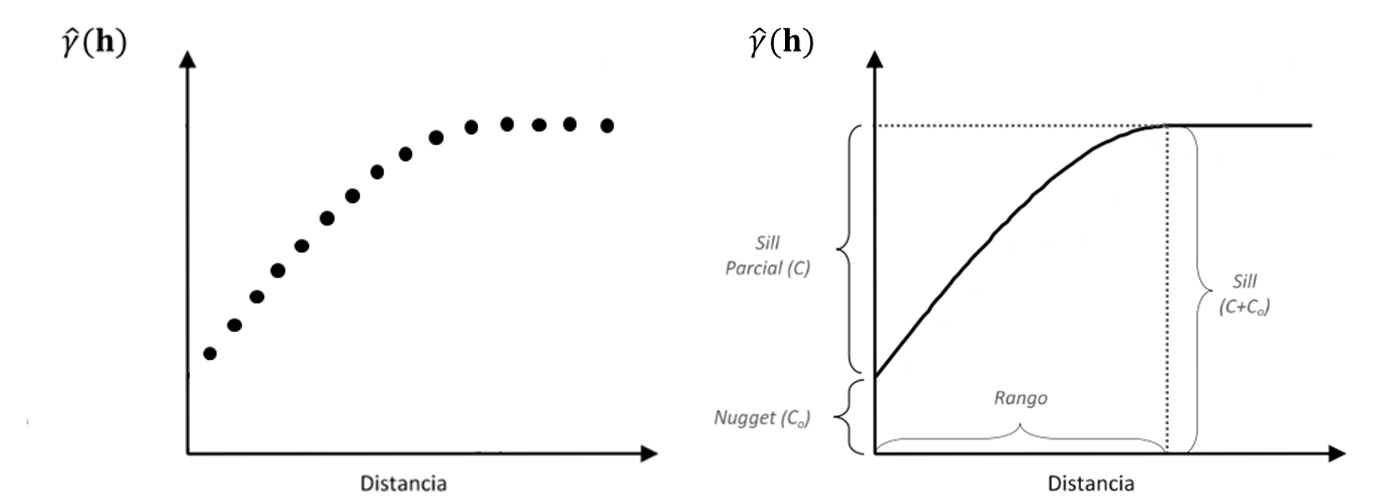
\includegraphics[width=\linewidth]{figuras/semivEmpTeo} 

}

\caption{a) Semivariograma empírico. b) Semivariograma teórico, modelo esférico. Se representan los tres parámetros que lo definen: rango, sill y efecto pepita o nugget.}\label{fig:semivariogramasej}
\end{figure}

En la práctica el semivariograma empírico \(\hat{\gamma}(h)\) puede no pasar a través del origen. La ordenada al origen del semivariograma representa a \(C_{0}\), por lo tanto \(C_0=\lim_{h\rightarrow0}{g(h)}\neq0\). Este parámetro representa la suma de errores aleatorios o no estructurados espacialmente, así como errores asociados con la variabilidad espacial a escalas más finas que la usada para realizar las mediciones. Un alto valor de \(C_0\) indica que la mayoría de la variación espacial no es explicada por el semivariograma. La varianza umbral o sill se obtiene sumando las varianzas antes mencionadas (\(C_0+C\)) y es la varianza de observaciones independientes, es decir observaciones que fueron tomadas a mayor distancia que \(R\).

Un semivariograma se define como anisotrópico si cambia en alguna forma respecto a la dirección que se considere. Si el semivariograma no solo depende de la longitud del vector h sino también de la dirección del vector entonces el semivariograma es anisotrópico. En los casos isotrópicos, los contornos de isocorrelación son esféricos, mientras que en el caso que haya anisotropía los contornos de isocorrelación son elípticos. Se reconocen dos tipos de anisotropía: anisotropía geométrica y anisotropía zonal. Anisotropía geométrica ocurre cuando el rango del semivariograma cambia en las distintas direcciones, pero no la varianza sill, por lo tanto, la correlación es más fuerte en una dirección que en otra. Anisotropía zonal existe cuando la varianza estructural del semivariograma cambia con la dirección. Anisotropía geométrica significa que la correlación es más fuerte en una dirección que en otra.

Una forma en que la anisotropía geométrica puede ser identificada es graficando un semivariograma experimental direccional. Diferencias en el semivariograma muestral usando diferentes ángulos al computarlo, es indicador de anisotropía. La anisotropía geométrica puede ser modelada cambiando el modelo de semivariograma por un proceso isotrópico transformando las coordenadas. Los modelos teóricos de semivariograma más usados en predicción espacial están basados son isotrópicos, por lo que es necesario una corrección en casos de anisotropía para poder utilizar la metodología clásica de predicción en geoestadística. El radio de anisotropía, es decir, el cociente entre los rangos de la dirección de máximo y mínima variación es usada para mesurar anisotropía. Algunos autores consideran que existe anisotropía significativa si el radio de anisotropía es mayor a 2,5.

\begin{figure}[H]

{\centering 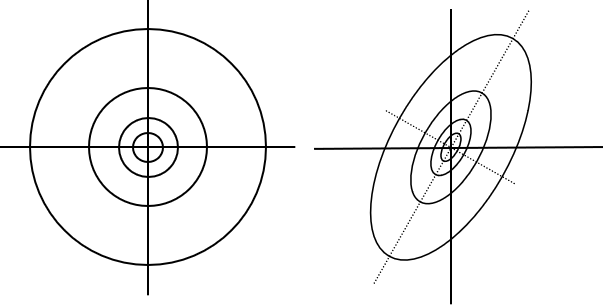
\includegraphics[width=\linewidth]{figuras/modeloIsoAniso} 

}

\caption{a) Modelo isotrópico. b) Modelo anisotrópico, con ángulo de anisotropía de 45º y un radio de anisotropía de 0,5.}\label{fig:modeloIsoAniso}
\end{figure}

En los procesos espaciales continuos, caracterizados por semivariogramas suelen obtenerse medidas del grado de estructuración espacial. Una de éstas es la varianza estructural relativa (RSV):

\[RSV=\Bigg(\frac{C}{C+C_0}\Bigg)\times100\%\]

Un valor alto de RSV indica que las predicciones geoestadísticas serán más eficientes que aquellas obtenidas con métodos de predicción que ignoran la información espacial. Un valor alto de RSV también indica una continuidad mayor del proceso espacial. Zimback (\protect\hyperlink{ref-Zimback_2001}{2001}) establece que el grado de dependencia espacial puede ser clasificado como: \(RSV \leq 25\%\) bajo, \(RSV\) entre \(25\%\) y \(75\%\) medio y \(RSV \geq 75\%\) alto. También se puede calcular el cociente \(\frac{C_0}{C_0+C}\) y en función de éste hablar de estructura espacial fuerte cuando el cociente es: \(\leq 25\%\), intermedia si el mismo se encuentra entre 25\% y 75\% y débil si el mismo es mayor al 75\%.

\hypertarget{ajuste-de-semivariogramas}{%
\subsection{Ajuste de semivariogramas}\label{ajuste-de-semivariogramas}}

El semivariograma empírico \(\hat{\gamma}(h)\), es un estimador insesgado de \(\gamma(h)\), pero provee solo estimaciones para un conjunto finito de distancias. Para obtener estimaciones de \(\gamma(h)\), para cualquier lag, al semivariograma empírico se le ajusta un modelo teórico. El análisis geoestadístico sigue entonces estos dos pasos: 1) obtención del semivariograma empírico y 2) ajuste de un modelo teórico de semivariograma al semivariograma empírico.

Las funciones que sirven como modelos teóricos de semivariograma deben ser condicionalmente definidas positivas. Existen varios modelos teóricos para funciones semivariogramas, entre los que se encuentran el modelo nugget, el lineal, el esférico, el gaussiano y el exponencial (Figura \ref{fig:figSemivariogramas}). El semivariograma de un proceso de ruido blanco (modelo nugget), donde los valores \(Z\left(s\right)\) se comportan como muestras aleatorias, todas con igual media y varianza sin correlación entre ellas. Este modelo suele ajustar el semivariograma empírico cuando la menor distancia de muestreo en los datos es mayor que el rango del proceso espacial.

\begin{figure}[H]

{\centering 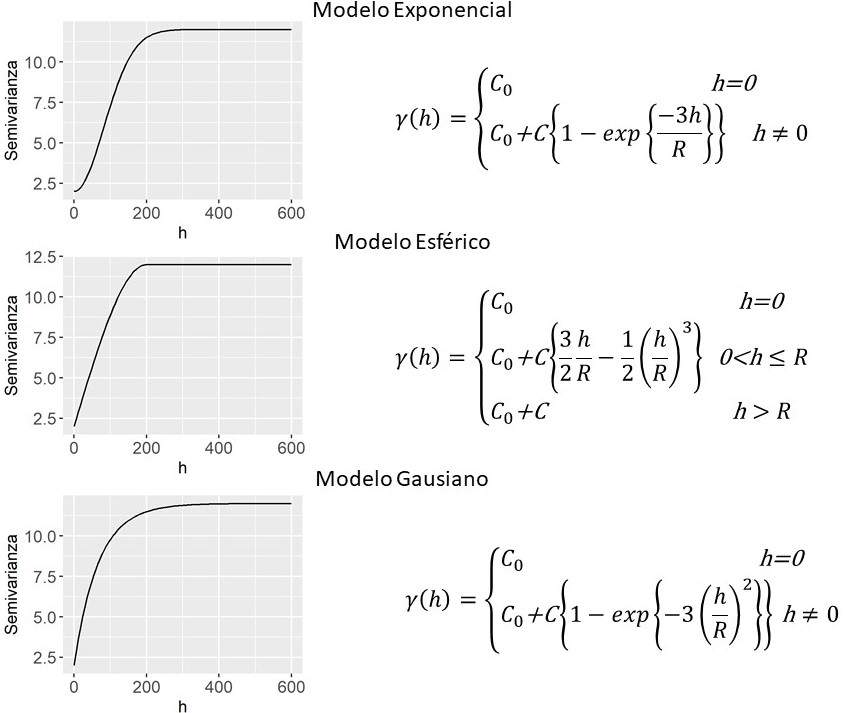
\includegraphics[width=\linewidth]{figuras/Semivariogramas} 

}

\caption{Funciones de semivariograma para el modelo exponencial, esférico y gaussiano. $C_0$=2, $C$=10 y $R$=200}\label{fig:figSemivariogramas}
\end{figure}

El modelo esférico es uno de los más populares entre los modelos de semivariograma. Tiene dos características principales: un comportamiento lineal cerca del origen y el hecho de que a la distancia \(R\) el semivariograma encuentra la meseta y después de esta se mantiene llano. El modelo exponencial se aproxima a la meseta del semivariograma asintóticamente cuando \(\parallel h \parallel\to\infty\). En la parametrización mostrada en la Figura \ref{fig:figSemivariogramas}, el parámetro \(R\) es el rango práctico del semivariograma. Frecuentemente el modelo puede encontrarse en una parametrización donde el exponente es \(-\parallel h \parallel / R\). Entonces el \(R_p\) corresponde a \(3R\). Para el mismo rango y meseta de un modelo esférico, el modelo exponencial alcanza el rango más rápidamente, es decir, a menor distancia que el modelo esférico. El modelo gaussiano exhibe un comportamiento cuadrático cerca del origen y produce una correlación de corto rango que son las más altas que para cualquier modelo estacionario de segundo grado con el mismo rango práctico. Además, es el más continuo cerca del origen de los considerados aquí. En la parametrización el rango práctico es \(\sqrt{3R}\).

Es importante notar que, si se realiza un análisis basado en semivariogramas y se pretende comparar los parámetros de los semivariogramas obtenidos bajo distintas condiciones, la utilización de modelos teóricos diferentes resulta poco útil. Hay que tener en cuenta que, por ejemplo, los rangos del modelo esférico y el exponencial no son directamente comparables. El modelo esférico es el único que tiene un umbral verdadero, ya que tanto el modelo exponencial como el gaussiano alcanzan el umbral de forma asintótica, o lo que es lo mismo, no lo alcanzan nunca y el modelo lineal no tiene umbral. En consecuencia, los rangos no son directamente equivalentes entre modelos. En este caso, es más conveniente elegir un único modelo para realizar comparaciones de procesos espaciales.

Los modelos de semivariograma son no lineales a excepción del modelo nugget. Por ello, para la estimación de parámetros estas funciones se usan métodos basados en aproximaciones numéricas. El método de ajuste por mínimos cuadrados ponderados (WLS) es común en la práctica. Para ello, se elige una función y valores iniciales de los parámetros basados en la observación del semivariogramas empírico. El tamaño del conjunto de datos a partir del cual el modelo de semivariograma es ajustado depende del número de \emph{lags} que se elija. Los valores de las clases de \emph{lag} en las cuál el número de pares no es mayor a 30 debieran ser removidos si se ajusta el semivariograma por mínimos cuadrados. Journel y Huijbregts 1978 recomiendan solo usar \emph{lags} menores a la mitad del máximo \emph{lag} en el conjunto de datos. La distribución de los puntos en el espacio determinará para qué \emph{lags} esto es posible.

\hypertarget{correlaciuxf3n-espacial-bivariada}{%
\section{Correlación espacial bivariada}\label{correlaciuxf3n-espacial-bivariada}}

\hypertarget{coeficiente-de-correlaciuxf3n}{%
\subsection{Coeficiente de correlación}\label{coeficiente-de-correlaciuxf3n}}

El coeficiente de correlación lineal de Pearson (\(r\)) es una medida de la magnitud de la correlación lineal entre dos variables. Para calcularlo se supone que se tiene una muestra aleatoria de unidades de análisis donde se han registrado simultáneamente dos variables. El intervalo de confianza para \(r\) y el valor \(p\) usados para decidir si la correlación poblacional entre ambas variables es cero o distinta de cero, dependen del tamaño de la muestra \(n\). El tamaño de la muestra es el número de unidades de análisis independientes.

Cuando las variables en estudio exhiben autocorrelación espacial, las observaciones de cada una de éstas estarán correlacionadas dentro de un determinado vecindario, es decir, no serán independientes entre sí. Luego, en el caso de datos espaciales, se viola la suposición de observaciones independientes para la prueba de significancia \(r\). Una propuesta para contemplar las correlaciones generadas por patrones espaciales es calcular el coeficiente de correlación haciendo un ajuste para determinar el número de observaciones independientes (tamaño de muestra efectivo) para acompañar la inferencia necesaria.

El coeficiente de correlación modificado (Clifford et~al., \protect\hyperlink{ref-Clifford_Richardson_Hemon_1989}{1989}; Dutilleul et~al., \protect\hyperlink{ref-Dutilleul_Clifford_Richardson_Hemon_1993}{1993}), permite evaluar correlación entre dos variables espacializadas en el mismo dominio espacial. La prueba se basa en la modificación de las varianzas y los grados de libertad de la prueba \(t\) estándar usada para evaluar significancia del coeficiente de correlación de Pearson y requiere de la estimación del tamaño efectivo de la muestra.

Considerando \(A \subset D\) un grupo de \(n\) sitios \(A={s_1, s_2,…,s_n}\), se supone que \(Z=Z(s_1), Z(s_2),…, Z(s_n)\) y \(Y= Y(s_1), Y(s_2),…,Y(s_n)\) con media constante y matriz de varianzas y covarianzas \(\Sigma_Z\) y \(\Sigma_Y\). Se divide \(D\) en los estratos \(D_0, D_1, D_2,…\). Entonces \(Cov(Z(s_i),Z(s_j))= C_Z(k)\) y \(Cov\big(Y(s_i),Y(s_j)\big)= C_Y(k)\), con \(s_i, s_j \in D_k\), para \(k= 0,1,…\) (Clifford et~al., \protect\hyperlink{ref-Clifford_Richardson_Hemon_1989}{1989}) sugieren como estimador de \(\hat{C}_Y(h)\)

\[ \hat{C}_Y(h) = \frac{\sum_{s_i,s_j \in A_k}{\big( Y(s_i) - \overline{Y} \big) \big( Y(s_j) - \overline{Y} \big)}} {n_k} \]

donde \(n_k\) es la cardinalidad de \(D_k\) y y similaridad para \(C_Z(k)\). Luego, Clifford et~al. (\protect\hyperlink{ref-Clifford_Richardson_Hemon_1989}{1989}) sugirió utilizar \(n^{-2}\sum_h{n_h\hat{C}_Z(h) \hat{C}_Y(h)}\)
Como un estimador de la varianza condicional de \(s_{ZY}=n^{-1} \sum_D{ \big(Z(s)-\overline{Z} \big) \big(Y(s)-\overline{Y} \big) }\). Como resultado se obtiene la prueba \(t\) modificada basada en el estadístico \(W\)

\[W=n \; s_{ZY} \Big( \sum_h{n_h \hat{C}_Z(h) \hat{C}_Y(h)} \Big)^{-2}\]

El cual a partir de una serie de aproximaciones a la varianza del coeficiente de correlación de Pearson (\(\sigma_r^2\)) entre los procesos \(Z(s)\) e \(Y(s)\) se puede escribir de la siguiente manera \(W=(\hat{M}-1)^{1/2}r\), \(\hat{M} = 1 + {\hat{\sigma}}_r^{-2}\) y \(\hat{\sigma}_r^2 = \frac{\sum_h{n_h \hat{C}_Z(h) \hat{C}_Y(h)}} {n^2 s_Z^2 s_Y^2}\).

Se define \(W\) como una prueba t modificada con \(\hat{M}-2\) grados de libertad, donde \(\hat{M}\) es el tamaño de muestra efectivo asumiendo bajo hipótesis nula la no correlación entre \(Z(s)\) e \(Y(s)\). Cuando se presenta una estructura de correlación espacial positiva, generalmente \(\hat{M} < n\), si existe estructura de autocorrelación negativa se espera que \(\hat{M} > n\).

\hypertarget{coeficiente-de-co-dispersiuxf3n}{%
\subsection{Coeficiente de co-dispersión}\label{coeficiente-de-co-dispersiuxf3n}}

Otra forma usada en estadística espacial para explorar patrones de correlaciones o covariaciones entre dos variables espacializadas, es el coeficiente de co-dispersión, que cuantifica la correlación entre dos procesos espaciales para un lag espacial particular sobre un espacio bidimensional. Para dos procesos espaciales intrínsecamente estacionarios \({Z(s):s\in D\subset R^2}\) y \({Y(s):s\in D\subset R^2}\) definidos en una parte de la región \(D\subset R^2\), el coeficiente de co-dispersión es definido como:

\[\rho_{ZY}(h)= \frac{E \Big[ \big(Z(s+h)-Z(s) \big) \big(Y(s+h)-Y(s) \big) \Big]}{\sqrt{E \big[Z(s+h)-Z(s) \big]^2 E \big[Y(s+h)-Y(s) \big]^2}}\]

La estructura de \(\rho_{ZY}\) es computacionalmente similar al coeficiente de correlación de Pearson. Al igual que ese coeficiente, \(\rho_{ZY}(h)\), donde los límites superior e inferior definen una asociación espacial negativa o positiva perfecta, respectivamente. Sin embardo, a diferencia del coeficiente de correlación de Pearson, \(\rho_{ZY}\) depende del lag \(h\), que enfatiza la idea de que la correlación espacial es un valor asociado con una distancia en el plano. El cálculo de la correlación se realiza para diferentes distancias y direcciones en el espacio. Cuando el coeficiente de co-dispersión se calcula para muchas direcciones, es útil mostrar esos valores en un solo gráfico. Vallejos et~al. (\protect\hyperlink{ref-Vallejos2015}{2015}) proponen el mapa de co-dispersión para resumir en un plano los valores de los coeficientes de co-dispersión obtenidos para distintos \emph{lag} espaciales (direcciones y distancias). El gráfico resume la información sobre la correlación entre dos procesos espaciales en forma radial sobre un plano que circunscribe los coeficientes en una semiesfera de radio no mayor al rango del proceso espacial \ref{fig:figGrafCoDisp}. En general las correlaciones espaciales que se observan desde un gráfico de co-dispersión permanecen ocultas en el análisis exploratorio usual y pueden ser distintas a las correlaciones lineales de Pearson no restringidas espacialmente. El gráfico de co-dispersión no debe ser confundido con un mapeo de la co-dispersión de las variables en el espacio de interés. No captura similitudes relacionadas con los patrones o formas que están presentes en los procesos espaciales, sino que captura la dependencia espacial entre los procesos para una distancia h. Los ejes del gráfico de co-dispersión hacen referencia a los \emph{lag} y direcciones y no a las coordenadas de los sitios muestrales originales.

\begin{figure}[H]

{\centering 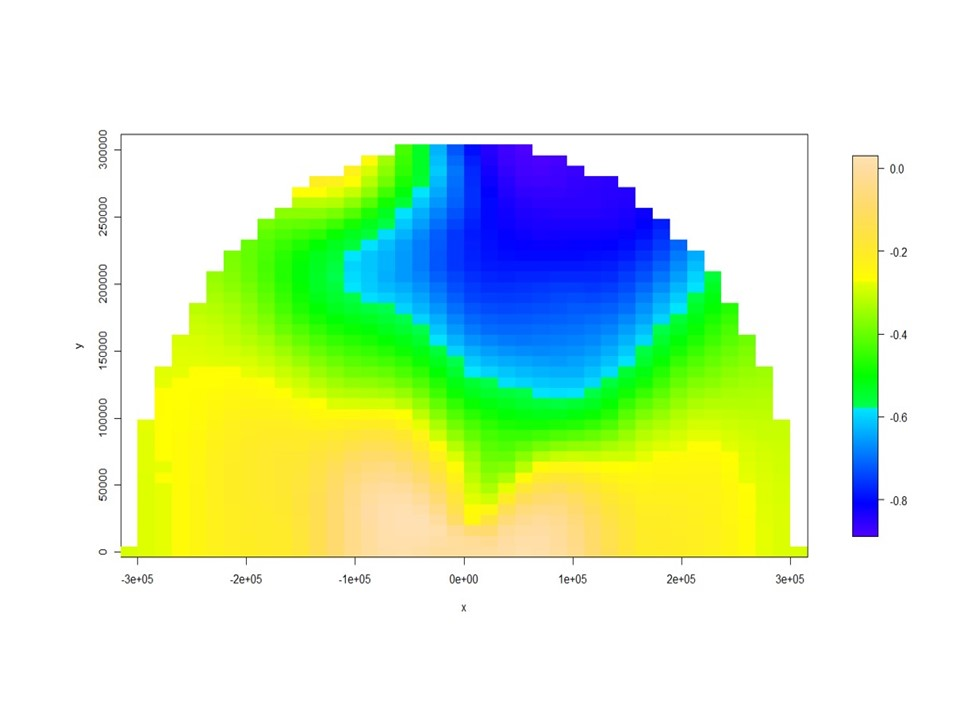
\includegraphics[width=\linewidth]{figuras/codispersion} 

}

\caption{Gráfico de co-dispersión mostrando la correlación espacial entre dos variables para varios lag espaciales.}\label{fig:figGrafCoDisp}
\end{figure}

\hypertarget{interpolaciuxf3n-kriging}{%
\section{Interpolación Kriging}\label{interpolaciuxf3n-kriging}}

La predicción espacial, es decir la predicción de valores de la variable en sitios del campo espacial donde no existen observaciones, usualmente se hace por el método kriging basándose en el semivariograma ajustado. Kriging proporciona el mejor estimador lineal insesgado del valor esperado para el sitio y un error de estimación conocido como varianza kriging. Esta varianza depende del modelo de semivariograma ajustado y de la ubicación en el espacio de los datos observados ya que son los datos observados en distintos sitios los que proveen información para aproximar el valor en el sitio sin dato. Las interpolaciones basadas en semivariograma, se denominan geoestadísticas y tienen ciertas ventajas respecto a interpolaciones determinísticas, como las obtenidas por el método IDW que se basa en las distancias geométricas entre los sitios con datos y el sitio a interpolar. Las observaciones que participan en la predicción se ponderan de forma distinta según la distancia estadística a la que se encuentran.

Los parámetros del semivariograma son los que gobiernan la asignación de los pesos o ponderaciones de las observaciones vecinas al sitio al cual se le asignará la predicción. El parámetro \emph{nugget} es determinante en la asignación de pesos. si la varianza del error es muy alta, todas las observaciones tenderán a tener el mismo peso en la interpolación. Por el contrario, si la varianza del error es baja, los coeficientes de ponderación serán distintos. Si el rango aumenta, cada punto tendrá mayor peso en la interpolación de otras observaciones. Entre los métodos de interpolación geoestadísticos que utilizan todos los datos simultáneamente se destacan los métodos de kriging ordinario, simple y universal. En el kriging ordinario la media de la variable es estimada localmente. En caso de conocer la media poblacional de la variable, hecho que raramente ocurre, se utiliza el kriging simple. En el kriging universal se estima también la influencia de una tendencia espacial de los datos. La predicción asignada a los puntos incógnita puede realizarse de manera puntual (kriging puntual) o definiendo bloques (kriging en bloques) (Schabenberger y Gotway, \protect\hyperlink{ref-Schabenberger_Gotway_2005}{2005}; Webster y Oliver, \protect\hyperlink{ref-Webster_Oliver_2007}{2007}).

\hypertarget{kriging-ordinario}{%
\subsection{Kriging ordinario}\label{kriging-ordinario}}

El kriging ordinario supone que la variación es aleatoria, que existe dependencia espacial y que el proceso espacial subyacente es intrínsecamente estacionario con media constante y varianza que depende solo de la separación en distancia entre los sitios y no de su posición. La predicción kriging resulta de una combinación lineal de los datos observados. Supongamos que los valores de \(Z\), han sido muestreados en los puntos \(s_1{,s}_2,\ldots,s_n\), para generar N datos \(z(s_i),\ i=1,\ 2,\ldots, N\). Para el caso del kriging ordinario puntual se predice \(Z\) en cualquier nuevo punto \(s_0\) mediante:

\[\hat{Z}(s_0)=\sum_{i=1}^{N}{w_iz(s_i)}\]

donde \(w\) son los pesos asignados a cada observación. Para asegurar que la estimación del valor esperado para el sitio sea insesgada y de mínima varianza, los pesos son dado de manera que:

\[\sum_{i = 1}^{N}{w_i=1}\]

\[E\big[\hat{Z}(s_0)-z(s_0)\big]=0\]

\begin{align*}
Var\big[\hat{Z}(s_0) \big] & = E\big[\hat{Z}(s_0) - z(s_0)^2 \big] \\&= 2\sum_{i=1}^{N}{w_i\gamma(s_i-s_0)-\sum_{i=1}^{N}\sum_{j=1}^{N}{w_iw_j\gamma(s_i-s_j)}}
\end{align*}

donde la cantidad \(\gamma(s_i - s_0)\) es la semivarianza de \(Z\) entre el punto de muestreo \(i\) y el punto objetivo \(x_0\) y \(\gamma(s_i - s_j)\) es la semivariancia entre los puntos de muestreo \(i\) y \(j\). Las semivarianzas se derivan del modelo teórico de semivariograma, debido a que no hay existen valores de semivarianzas entre los sitios con datos y los sitios objetivos donde no existen valores observados. Si un sitio objetivo también es un punto de muestreo, el kriging puntual devuelve el valor observado en ese sitio y la varianza de estimación es cero. El kriging puntual es un interpolador exacto en este sentido. El siguiente paso en kriging es encontrar los pesos que minimizan la varianza de la predicción sujeto a la restricción de que la suman de los pesos se igual a 1.

\[\sum_{i=1}^{N}w_i\gamma(s_i-s_0)+\psi(s_0)=\gamma(s_j-s_0) \forall j\]

La cantidad \(\psi (s_0)\) es el multiplicador de Lagrange introducido para lograr la minimización. La solución de las ecuaciones de kriging proporciona los pesos para las ponderaciones y la varianza de predicción se obtiene de la siguiente forma:

\[\sigma^2(s_0)=\sum_{i=1}^{N}{w_i\gamma(}s_i-s_0)+\ \psi(s_0)\]

\hypertarget{kriging-en-bloques}{%
\subsection{Kriging en bloques}\label{kriging-en-bloques}}

El kriging en bloques consiste en estimar directamente el valor promedio de la variable sobre un soporte mayor que el soporte de los datos (bloque). Intuitivamente, la idea es calcular mediante kriging puntual los valores en todos los puntos de una superficie o bloque y usar la media de las predicciones como estimador del valor esperado para el sitio. La estimación para cualquier bloque sigue siendo un promedio ponderado de los datos, \(z\ (s_1),\ z\ (s_2),\ ...,\ z\ (s_N)\):

\[\hat{Z}(B)=\sum_{i=1}^{N}{w_iz(s_i)}\]

Los factores de ponderación se obtienen nuevamente para minimizar la varianza del error y para obtener un estimador insesgado de la media. La grilla de predicción sobre la que se construye el mapa de variabilidad espacial presenta una dimensión menor que la de los bloques, asegurándose la obtención de un mapa más suavizado respecto al obtenido con kriging puntual. El kriging en bloques ha mostrado ser efectivo a la hora de reducir errores que pueden trasladarse en los mapas como consecuencia de inexactitudes de datos puntuales.

\hypertarget{kriging-local}{%
\subsection{Kriging local}\label{kriging-local}}

Hemos dicho que los pesos de las observaciones en la predicción geoestadística son funciones de las semivarianzas entre las observaciones en sitios en el vecindario, \(\gamma(s_i-s_j)\), y entre cada punto de muestreo y el punto a predecir, \(\gamma(s_i-s_0)\). En general solo los puntos cercanos al punto a predecir tienen un peso significativo. Cuando la relación nugget:sill es pequeña el interpolador kriging es visto como un predictor local, donde para la predicción de \(Z(s_0)\) participarán sólo datos de puntos dentro de la proximidad de \(s_0\) (\emph{kriging neighborhood} o kriging local). El kriging local esencialmente asigna pesos \(w(s_0)=0\) para todos los puntos \(s_i\) fuera de la zona en la que se quiere predecir. Por otra parte, esto permite que podemos aceptar el supuesto de estacionariedad local (o cuasi estacionariedad), es decir se puede restringir el supuesto de estacionariedad de la media a los vecindarios del kriging. Lo que sucede en distancias mayores a las del vecindario del sitio no será de importancia para la predicción en el sitio. La predicción y varianza kriging dependen principalmente de la parte del semivariograma cercana al origen, por ello es de importancia modelar bien el semivariograma en estos lugares, \emph{i.e.} dar más peso a las semivarianzas experimentales cercanas al origen. No hay reglas para definir el vecindario para implementar el kriging local, aunque cuando el nugget es relativamente bajo se pude definir un radio de vecindad cercano al rango o rango práctico del modelo de semivariograma ajustado. Cuando el efecto nugget es importante el radio de vecindad debería ser mayor al rango ya que es probable que puntos más distantes tengan aún peso significativo. Otra alternativa para definir el vecindario se basa en términos de un número mínimo y máximo de datos cercanos al punto a predecir. Algunos autores recomiendan utilizar un mínimo de 7 vecinos y un máximo de 20.

\hypertarget{kriging-universal}{%
\subsection{Kriging universal}\label{kriging-universal}}

La suposición de estacionariedad intrínseca no se cumple cuando existen tendencias geográficas pronunciada de naturaleza sistemática y no aleatoria. La tendencia puede ser regional, es decir, una variación sistemática en toda la región de interés o local de un punto a otro dentro de la región estudiada. La existencia de tendencias puede ser explorada graficando los datos de la variable analizada en función a la variable que se supone genera la tendencia espacial. La tendencia también se manifiesta en los semivariogramas experimentales con un incremento de la semivarianza con la distancia que no tiene límites. Si hay tendencia, entonces \(\mu\) ya no es constante, sino que depende de s. Además, el semivariograma experimental de los datos ya no estima el semivariograma de los errores aleatorios, \(\varepsilon(s)\). Se necesita estimar el semivariograma de \(\varepsilon(s) = Z (s) - \mu(s)\). Cuando este variograma es el input del kriging, el proceso de interpolación se conoce como ``kriging universal'' y la predicción se obtiene como:

\[\hat{Z}(s_0)=\sum_{i=1}^{N}{w_i \; f_kz(s_i)}\]

donde \(f_k\) es función de las coordenadas espaciales.

\hypertarget{validaciuxf3n-cruzada}{%
\subsection{Validación cruzada}\label{validaciuxf3n-cruzada}}

La predicción implica asignar nuevos valores de las variables respuesta a contextos o escenarios que no corresponden al conjunto de escenarios medidos, es decir no se trata de aquellos sitios que utilizaron para realizar la predicción espacial. Entre las alternativas para estimar la exactitud de la predicción existen las técnicas de validación cruzada o técnicas de partición del conjunto de datos en datos de calibración y datos de validación (Efron y Hastie, \protect\hyperlink{ref-Efron_Hastie_2016}{2016}). Es necesario identificar un grupo de observaciones sobre las que se ajustará el modelo o el método que permite predecir, usualmente llamado datos de calibración, y otro grupo que se usará para validar, llamado datos de validación. El modelo (semivariograma teórico) se ajusta sobre el conjunto de datos de entrenamiento y posteriormente se usa para la predicción de interés, con observaciones del subconjunto de validación. Seguidamente, los valores observados del conjunto de validación se comparar con los valores predichos por el modelo. Usualmente el proceso se repite cruzando el rol de los subconjuntos de datos, es decir el que era de validación pasa a ser de calibración y viceversa.

Sin embargo, otras estrategias pueden ser usadas para la selección de los datos de entrenamiento y validación. Una es particionar en forma aleatoria los datos en ambos conjuntos. Otro tipo de validación cruzada es dejando uno fuera (\emph{Leave-One-Out}) donde se utiliza una sola observación para conformar el subconjunto de validación y se deja al resto como subconjunto de entrenamiento. El modelo se ajusta utilizando las \(n – 1\) observaciones de entrenamiento y se obtiene una predicción para la observación excluida. Este proceso se repite \(n\) veces. Otro tipo de validación cruzada es \(k-fold\), donde las observaciones se dividen aleatoriamente en \(k\) grupos de aproximadamente igual tamaño. Uno de los \(k\) grupos se emplea como subconjunto de validación, mientras que el resto de los grupos se emplean para entrenar el modelo. El proceso de validación cruzada es repetido durante k iteraciones, con cada uno de los subconjuntos de datos de prueba. Un valor común de \(k\) que puede dar buenos resultados en cuanto al equilibrio sesgo-varianza para estimar el error de predicción es \(k=10\). Si el modelo tuvo un buen desempeño, los residuos de la validación cruzada serán pequeños, su media será cercana a cero y no presentarán estructura.

En la evaluación de modelos geoestadísticos, los valores predichos de kriging \(\hat{Z}(s_i)\) se comparan con los observados \(z(s_i)\), y se calcula una medida resumen que caracteriza el resultado de la comparación. Algunas de estas medidas resumen son:

Error medio

\[ME=\frac{1}{N}\sum_{i=1}^{N}\big\{z(s_i)-\hat{Z}(s_i)\big\}\]

donde \(N\) es el número de observaciones, \(z(s_i)\) es el valor verdadero en \(s_i\) y \(\hat{Z}(s_i)\) es el valor predicho en ese punto.

Error cuadrático medio (Mean Square Error, MSE):

\[MSE=\frac{1}{N}\sum_{i=1}^{N}{\big\{z(s_i)-\hat{Z}(s_i)\big\}^2}\]

Raíz del error cuadrático medio:

\[RMSE=\frac{1}{N}\sqrt{\sum_{i=1}^{N}\big\{z(s_i)-\hat{Z}(s_i)\big\}^2}\]

Media del cociente del error cuadrático (Mean Squared Deviation Ratio, MSDR):

\[MSDR=\frac{1}{N} \sum_{i=1}^{N}\frac{ \big\{ z(s_i) - \hat{Z}(s_i) \big\}^2} {\hat{\sigma}^2(s_i)}\]

donde \(\hat{\sigma}^2(s_i)\) es la varianza de la predicción kriging en el punto \(s_i\).

Para el caso de datos espaciales, no solo es necesario disponer de una medida de error de predicción global, sino que también hay que evaluar del error de la predicción en cada sitio específico, \emph{i.e.} dimensionar el error puntual de la predicción espacial.

\hypertarget{caracterizaciuxf3n-de-variabilidad-espacial-con-muxfaltiples-capas-de-datos}{%
\chapter{Caracterización de variabilidad espacial con múltiples capas de datos}\label{caracterizaciuxf3n-de-variabilidad-espacial-con-muxfaltiples-capas-de-datos}}

\hypertarget{anuxe1lisis-de-componentes-principales}{%
\section{Análisis de componentes principales}\label{anuxe1lisis-de-componentes-principales}}

Diferentes objetivos pueden surgir cuando analizamos un conjunto de datos que además de ser espaciales o georreferenciados es multivariado (\emph{i.e.} múltiples capas de información sobre el mismo dominio espacial o varias variables por sitio). Por un lado, se puede querer resumir la variabilidad de los sitios usando unas pocas variables sintéticas que representen bien la variabilidad en las variables originales. Por otro, se puede querer resumir patrones espaciales usando unas pocas variables sintéticas que combinan las múltiples capas de información considerando la correlación espacial subyacente. Una solución al primer problema es usar el Análisis de Componentes Principales (PCA (Pearson, \protect\hyperlink{ref-F.R.S._1901}{1901})). Mientras que el segundo objetivo puede ser abordado mediante el Análisis de Componentes Principales Espaciales propuesto por (Dray et~al., \protect\hyperlink{ref-Dray_Sauxefd_Duxe9bias_2008}{2008}), también conocido como MULTISPATI-PCA. Éste se basa en el PCA, pero incorpora la restricción dada por los datos espaciales mediante el cálculo del índice de Moran antes de obtener las variables sintéticas o componentes principales (PC).
Los datos multivariados son generalmente registrados en una matriz \(X\) con \(n\) filas (observaciones) y \(p\) columnas (variables). El PCA permite identificar las variables que explican la mayor parte de la variabilidad total contenida en los datos, explorar las correlaciones entre variables y reducir la dimensión del análisis al combinar las variables originales en nuevas variables sintéticas. El PCA opera sobre la matriz de covarianza de las variables originales o de las variables estandarizadas con el fin de encontrar una base ortogonal de tal manera que el primer eje del nuevo espacio considera la dirección de mayor variación de los datos originales. La descomposición espectral de la matriz de covarianzas proporciona un conjunto de autovectores y sus correspondientes autovalores. Los autovectores contienen los coeficientes de ponderación para construir variables sintéticas como combinaciones lineales de las variables originales. Los coeficientes de cada variable en estas combinaciones lineales indican la importancia relativa de las variables para explicar la variabilidad entre las observaciones. Las combinaciones lineales obtenidas con PCA se llaman componentes principales (PC), son ortogonales y en conjunto explican la variabilidad de los datos originales. Existen tantas PC posibles de formar como columnas en la matriz \(X\). La primera componente (PC1) explica la mayor parte de la variación en el conjunto de datos y la segunda (PC2), la mayor parte de la variabilidad remanente o no explicada por la PC1, y así sucesivamente.

Los resultados del PCA se pueden visualizar en un gráfico denominado Biplot (Gabriel, \protect\hyperlink{ref-Gabriel_1971}{1971}) el cual permite representar en un plano óptimo para el estudio de variabilidad, las diferencias entre sitios, la correlación entre variables y las variables que mejor explican las principales componentes de variabilidad. La incorporación de la información geográfica o la característica espacial de los datos suele realizarse a posteriori del PCA mediante la asignación de los valores de las componentes a cada uno de los sitios georreferenciados o ajustando semivariogramas a las PC.

El objetivo de MULTISPATI-PCA, otra forma de trabajar con datos espaciales, es encontrar variables sintéticas independientes que optimicen el producto de la varianza total y la autocorrelación espacial. Para delimitar los vecindarios, MULTISPATI-PCA utiliza una matriz de pesos espaciales determinando cuáles y cuántas observaciones cercanas a cada sitio deben ser consideradas para el cálculo del índice de autocorrelación espacial. Este análisis permite estudiar las relaciones entre las variables considerando su estructura espacial. Para la implementación del análisis es necesario primero definir cómo la información espacial será incorporada. En MULTISAPTI - PCA, la detección de la estructura espacial se realiza a través del índice de Moran. Es necesaria la construcción de una red de conexión (también llamada gráficos de vecinos) la cual usa un criterio objetivo para definir que entidades son vecinas y cuáles no. Existen diferentes opciones o alternativas metodológicas para definir los vecindarios que dependen de los diferentes tipos de arreglos espaciales presente en los datos. Para muestreos irregulares los vecindarios suelen definirse a partir de la red de conexión propuesta por Gabriel (Gabriel y Sokal, \protect\hyperlink{ref-Gabriel_Sokal_1969}{1969}), mediante la triangulación de Delaunay (Lee y Schachter, \protect\hyperlink{ref-Lee_Schachter_1980}{1980}). Otro método es el de los vecinos más cercanos (Cover y Hart, \protect\hyperlink{ref-Cover_Hart_1967}{1967}) o el basado en la especificación de una distancia como radio del vecindario de cada sitio.

Una vez que la red de conexión es definida, la información espacial es almacenada en una matriz de conexión binaria \(C\) (en la cual \(c_{ij}=1\) si las unidades espaciales \(i\) y \(j\) son vecinas o \(c_{ij}=0\) en caso contrario), la cual es simétrica y tiene tantas filas y columnas como sitios. Esta matriz de conectividad \(C\) en general es escalada para obtener la matriz de pesos espaciales (representación matemática de la disposición geográfica de los sitios en el dominio espacial). Los pesos espaciales reflejan a priori la ausencia \((w_{ij}=0)\), presencia \((w_{ij}=1)\) o intensidad \((w_{ij}>0)\) de la relación espacial entre los sitios. Una vez que los pesos espaciales han sido definidos, el índice de autocorrelación de Moran es computado.

El método MULTISPATI-PCA opera sobre la matriz \(\widetilde{X}=WX\) que está compuesta por los promedios ponderados de los valores de los vecinos de cada sitio según indique la matriz de conexión espacial, esta matriz es llamada matriz lagged. Las dos matrices \(X\) y \(\widetilde{X}\) tienen las mismas cantidades de columnas (variables) y de filas (sitios). El análisis MULTISPATI-PCA consiste en analizar la correlación entre este par de matrices (\(\widetilde{X}\) y \(X\)) mediante un análisis de co-inercia (Dray et~al., \protect\hyperlink{ref-Dray_Chessel_Thioulouse_2003}{2003}). MULTISPATI-PCA maximiza el producto escalar entre una combinación lineal de las variables originales y una combinación lineal de variables \emph{lagged}. La ventaja de MULTISPATI-PCA respecto al PCA es que las componentes principales espaciales del MULTISPATI-PCA (sPC) contemplan la autocorrelación espacial entre los sitios, maximizándola en las primeras componentes. Por lo tanto, las primeras sPC del MULTISPATI-PCA muestran fuertes estructuras espaciales o altos índices de autocorrelación y no sólo mayores varianzas como en el PCA clásico. El método MULTISPATI-PCA constituye una herramienta multivariada útil no sólo para mapear la variabilidad conjunta de múltiples capas de datos dentro del dominio espacial estudiado sino también para la delimitación de zonas o áreas homogéneas en sentido multivariado cuando las componentes espaciales se usan como inputs de algoritmos de clasificación.

\hypertarget{anuxe1lisis-de-conglomerados}{%
\section{Análisis de conglomerados}\label{anuxe1lisis-de-conglomerados}}

Los métodos multivariados, utilizados para la clasificación de sitios de un dominio espacial, suelen basarse en algoritmos de agrupamiento no supervisados como los algoritmos de conglomerados jerárquicos o en algoritmos de conglomerados no jerárquico como k-means o fuzzy k means. Contrariamente al algoritmo k-means u otros métodos determinísticos de agrupamiento en los que cada observación sólo puede pertenecer a un único clúster, los métodos de clasificación basados en la teoría difusa (como fuzzy k-means), permiten que cada observación pueda asignarse a más de un clúster, con diferentes grados de pertenencia para cada clúster. Aplicado a datos espaciales puede generar alta fragmentación ya que el algoritmo de agrupación no tiene en cuenta la información espacial asociada a cada observación. Frogbrook y Oliver (\protect\hyperlink{ref-Frogbrook_Oliver_2007}{2007}) y Milne et~al. (\protect\hyperlink{ref-Milne_Webster_Ginsburg_Kindred_2012}{2012}) propusieron introducir la restricción espacial mediante la incorporación de nuevas variables asociadas a parámetros del variograma co-regionalizado o del variograma de la componente principal de las variables originales. Córdoba et~al. (\protect\hyperlink{ref-Cuxf3rdoba_Balzarini_Bruno_Costa_Balzarini_Costa_2012}{2012}) propusieron implementar fuzzy k means usando las componentes principales espaciales como variables de entrada para la clasificación con datos espaciales, logrando así disminuir la fragmentación e incrementar la contigüidad de los conglomerados espaciales. Otra alternativa, para delimitar conglomerados espaciales es aplicar filtros espaciales a la clasificación resultante de un método de clasificación estándar (Galarza et~al., \protect\hyperlink{ref-Galarza_Mastaglia_Albornoz_Martux131nez_2013}{2013}; Ping y Dobermann, \protect\hyperlink{ref-Ping_Dobermann_2003}{2003}).

En el método fuzzy k-means además de la matriz de datos \(X\) se genera la matriz de pertenencia difusa \(U\), que contiene los valores o asignaciones parciales de cada una de las n observaciones en cada uno de los k clusters o conglomerados, con la restricción que se debe cumplir para cualquier \(i = 1,\ldots,n\) y para cualquier \(j = 1,\ldots,k\):

\[u_{ij}\in[0,1]\ \forall_i,_j\]

\[\sum_{j=1}^{k}{u_{ij}=1,\ \forall_j}\]

La partición difusa óptima de los datos es la que minimiza la función objetivo \(j_m\) igual a la suma ponderada de las distancias cuadráticas entre las observaciones y los centroides de cada clúster que conforman la matriz \(V\):

\[j_m(U,V)=\sum_{i=1}^{n}\sum_{j=1}^{k}(u_{ij})^m(d_{ij})^2\]

donde \(m\) es el coeficiente de ponderación difuso (\(1\le\ m\ < \infty)\) cuya función es controlar el grado de solapamiento que se establece entre los clusters y \({{(d}_{ij})}^2\) es el cuadrado de la distancia en el espacio de los atributos entre el punto \(i\) y la clase centroide \(j\). Distintas métricas de distancia pueden ser usadas. La distancia Euclídea se utiliza cuando las variables son independientes y de igual varianza. En caso contrario la distancia de Mahalanobis es usada. El algoritmo difuso \emph{fuzzy k-means} utiliza un proceso iterativo que hace óptima la partición difusa de los datos \(X\). La estructura del algoritmo (Bezdek et~al., \protect\hyperlink{ref-Bezdek_Coray_Gunderson_Watson_1981}{1981}) es la misma para cualquier conjunto de variables de entrada. Cuando el algoritmo ha asignado pesos o probabilidades de pertenencia a cada grupo para cada observación, se computaban una serie de índices para validar los distintos arreglos de conglomerados.

Para evaluar la clasificación conseguida con un determinado número de grupos, existen diferentes índices como el coeficiente de partición (o fuzziness performance index-FPI, (Bezdek et~al., \protect\hyperlink{ref-Bezdek_Coray_Gunderson_Watson_1981}{1981})), el índice de entropía de la clasificación o \emph{normalized classification entropy} (NCE, (Bezdek et~al., \protect\hyperlink{ref-Bezdek_Coray_Gunderson_Watson_1981}{1981})), el índice de Xie-Beni (Xie y Beni, \protect\hyperlink{ref-Xie_Beni_1991}{1991}) y el de Fukuyama-Sugeno (Fukuyama y Sugeno, \protect\hyperlink{ref-Fukuyama_Sugeno_1989}{1989}), entre otros.

El coeficiente de partición (CP) mide el grado de solapamiento (grado de fuzziness) entre los grupos formados. Se considera que mientras menos difusa es la partición, mejor es la clasificación. Por tanto, se prefiere la estructura con un número de conglomerados para la cual el coeficiente de partición es mayor. El máximo equivale a una clasificación en la que cada observación pertenece a un único clúster. El mínimo se da cuando cada observación pertenece, con la misma probabilidad, a cada clúster (mayor incertidumbre).

Otro índice que se puede usar para decidir con cuantos conglomerados quedarse es el conocido como entropía de la partición (EP) que cuantifica el grado de desorganización de la clasificación. Para este índice los valores próximos a 0 son indicativos de una mejor clasificación, es decir, con mayor grado de organización o menos difusos. El índice de Xie-Beni (XB) evalúa el cociente entre las distancias intracluster e intercluster. Se prefieren particiones donde la distancia intra-cluster es mínima y la distancia inter-cluster máxima. El índice XB es considerado como una medida de compacidad. Un valor bajo de XB, representa una clasificación con grupos compactos y separables. Por consiguiente, la mejor partición se obtiene mediante la minimización de XB. El índice Fukuyama-Sugeno (FS) es función de la separación entre los centroides de los grupos y la media de todos los centroides. El mínimo de FS corresponde a una partición con clases compactas y separables. Es importante considerar que, para un conjunto de datos, los índices no son necesariamente consistentes entre sí sugiriendo diferentes números de clúster como partición óptima. Una propuesta es promediar el valor de estos índices normalizados por el máximo usando para CP su reciproco, \(CP^*=1/CP\) , para que el valor mínimo en todos los índices represente la estructura optima.

\hypertarget{predicciuxf3n-con-muxfaltiples-capas-de-datos}{%
\chapter{Predicción con múltiples capas de datos}\label{predicciuxf3n-con-muxfaltiples-capas-de-datos}}

La predicción del valor de una variable en un sitio no observado, realizada por interpolación kriging local, se alimenta de datos de la misma variable que se quiere predecir, pero obtenidos en sitios del vecindario de aquel para el que se requiere la predicción. Aún cuando la predicción pueda ser óptima, resulta informativo conocer el impacto de otras variables (variables secundarias, auxiliares o explicativas) sobre la predicción.

El método conocido como regresión kriging (Hengl et~al., \protect\hyperlink{ref-Hengl_Heuvelink_Rossiter_2007}{2007}) permite predecir o interpolar los valores de una variable en sitios no muestreados que se encuentran entre los sitios con observaciones a partir de capas de datos secundarios que actúan como variables predictoras. La incorporación de covariables de sitio puede mejor sustancialmente la predicción de una variable respuesta espacializada. Para tal fin es necesario el ajuste de un modelo de regresión múltiple que describe la relación entre la variable observada y las capas de variables predictoras. Luego de ajustar la regresión, se obtienen los residuos (diferencia entre valor observado y valor predicho por el modelo a partir de las variables secundarias) y se realiza una interpolación kriging sobre los residuos para contemplar la espacialidad que no se encuentra relacionada con las capas de información usadas en el ajuste previo. Finalmente, los resultados del ajuste de regresión y de la interpolación kriging son combinados para producir la predicción.

Matemáticamente, esta interpolación es equivalente a la que hemos llamado kriging universal, ya que allí se realiza un ajuste de la variable de interés y las coordenadas espaciales (un tipo de variable auxiliar) cuyo impacto es descontado antes de realizar la interpolación espacial. Kriging desde modelo de regresión es también equivalente matemáticamente al método de interpolación conocido como kriging con deriva externa donde múltiples variables auxiliares son usadas como predictoras (covariables de sitio que son externas o distintas a las coordenadas espaciales) e intervienen directamente para resolver los pesos de la interpolación espacial.

La predicción sitio-especifica de una variable respuesta en función de covariables de sitio puede realizarse también desde el marco teórico de los modelos lineales mixtos de covarianza residual (Balzarini et~al., \protect\hyperlink{ref-Balzarini_Macchiavelli_Casanoves_2004}{2004}). Es decir, ajustando un único modelo, donde la componente determinística es un modelo de regresión lineal múltiple que relaciona la respuesta con las covariables de sitio y las componentes sistemáticas (patrón espacial) y estocástica (variación sin estructura) de la variación espacial son expresadas conjuntamente en la matriz de varianza y covarianza de los términos de error (matriz de covarianza residual). Bajo este marco teórico, se utiliza máximo verosimilitud restringida o REML (Patterson y Thompson, \protect\hyperlink{ref-Patterson_Thompson_1971}{1971}) para estimar el modelo predictivo. El modelo relaciona la variable de interés para el estudio de variación espacial con las variables explicativas también distribuidas espacialmente y contemple la dependencia espacial en las observaciones de la variable a predecir incorporando en la matriz de covarianza residual covariaciones derivadas de una función basada en la distancia que separa dichas observaciones en el espacio.

La construcción de un modelo predictivo para datos espaciales también puede realizarse desde un marco teórico Bayesiano, donde sistemática relacionada con la media de la respuesta sigue siendo el modelo de regresión lineal múltiple, pero se incorporan parámetros aleatorios de sitio para modelar la componente sistemática de los datos espaciales, los cuales se predicen independientemente de la componente de error. Trabajar el efecto de sitio como aleatorio, junto a la suposición de procesos espaciales locales, ha permitido eficientizar la estimación en un único paso de modelos para datos espaciales. Bajo el marco teórico bayesiano y el supuesto de campo aleatorio gaussiano markoviano para el proceso espacial, la estimación por aproximación de Laplace anidada conocida como INLA (del término en inglés \emph{Integrated Nested Laplace Aproximation}) es uno de los métodos elegidos para ajustar el modelo espacial (Rue et~al., \protect\hyperlink{ref-Rue_Martino_Chopin_2009}{2009}).

Alternativamente, la construcción del modelo predictivo espacial puede realizarse mediante métodos de aprendizaje automático, también bajo el concepto de ajustar un modelo para la componente determinística, obtener los residuos y modelar el proceso espacial en los residuos para finalmente combinar ambos resultados (Li et~al., \protect\hyperlink{ref-Li_Heap_Potter_Daniell_2011}{2011}). Los modelos basados en árboles de regresión (Breiman et~al., \protect\hyperlink{ref-Breiman_Friedman_Olshen_Stone_2017}{2017}) son particularmente útiles para abordar la primera etapa, aquella donde la variable respuesta es relacionado con las múltiples covariables que definen capas de información espacial.

Cualquiera sea la aproximación usada en la construcción del modelo para realizar la predicción espacial y posterior mapeo de la variable respuesta, para lograr buenos resultados se requiere hacer uso del criterio experto en la disciplina, realizar un adecuado preprocesamiento de los datos, identificar los predictores influyentes y validar el modelo estimado (Kuhn y Johnson, \protect\hyperlink{ref-Kuhn_Johnson_2013}{2013}).

La validación cruzada es una técnica de amplio uso para evaluar el desempeño de modelos predictivos con múltiples capas de información. La forma más adecuada de muestrear para dividir el conjunto de datos en estudio y los criterios de validación es discutida (Brenning, \protect\hyperlink{ref-Brenning_2012}{2012}; Efron y Tibshirani, \protect\hyperlink{ref-Efron_Tibshirani_1997}{1997}), pero como regla general se puede establecer que en cuanto menor es la proporción de datos que conforma el subconjunto de validación, menor capacidad de extrapolación tendrá el modelo ajustado y que éste no puede crecer indefinidamente ya que también se requiere buen tamaño del subconjunto de calibración para ajustar un buen modelo. El compromiso se relaja a medida que la base de datos observados es de mayor tamaño.

Una medida comúnmente usada en la evaluación de modelos de regresión lineal estimados por mínimos cuadrados es el \(R^2\) o coeficiente de determinación. Éste expresa la bondad del ajuste del modelo respecto a los datos observados más que la capacidad predictiva que interesa evaluar cuando el modelo es usado como predictor. Otras medidas de bondad de ajuste, como los criterios de información de Akaike y BIC usados para evaluar modelos lineales de covarianza residual estimados por métodos basados en la verosimilitud o DIC usado en contextos de ajustes de modelos bayesianos, permite calificar el ajuste del modelo a los datos observados, pero no su desempeño para predecir observaciones no realizadas. La validación cruzada es, por el contrario, una estrategia transversal a distintas aproximaciones metodológicas o marcos teóricos que provee información de la capacidad predictiva del modelo, y por tanto una medida de cómo podría funcionar en la interpolación espacial. No obstante, es de resaltar que un buen modelo predictivo debería representar también un buen ajuste de los datos de entrenamiento, y por ello métricas comunes de bondad de ajuste suelen ser usadas para una primera selección de modelos predictivos.

\hypertarget{regresiuxf3n-con-errores-correlacionados-espacialmente-vuxeda-reml}{%
\section{Regresión con errores correlacionados espacialmente vía REML}\label{regresiuxf3n-con-errores-correlacionados-espacialmente-vuxeda-reml}}

Se asume una relación lineal determinística entre la variable respuesta y las covariables espacializadas que se modela a través de coeficientes de regresión, y el proceso espacial subyacente en los datos se modela sobre los términos de error del modelo. Éstos, en lugar de considerarse independientes como en aproximaciones estadísticas clásicas, se suponen espacialmente correlacionados, \emph{i.e.} con correlaciones entre pares de términos de error expresadas como función de la distancia que separa los sitios desde los que se obtuvieron las observaciones. La varianza residual del modelo mide la variabilidad no estructurada espacialmente y caracteriza la componente estocástica del modelo. Se ajusta un modelo directamente a los datos, y no a las semivarianzas como en la geoestadística clásica. La estructura de covariación espacial se define en función de la distancia entre las observaciones al igual que en la geoestadística, pero se estima simultáneamente con los parámetros del modelo de regresión, \emph{i.e.} los coeficientes de regresión que interpretan como pendientes o cambios en la respuesta por unidad de cambio de la covariable de sitio.

El modelo de regresión lineal múltiple con errores correlacionados espacialmente para una variable \(Y\) asume la siguiente distribución para la \emph{i-ésima} observación:

\[Y_i\sim N \big(E(Y),V(Y) \big)\]

\[Y_i=\beta_0+\sum_{j=1}^{p}{x_{ij}\beta_j}+\varepsilon_i\]

\[\varepsilon(s_i)\sim N(0,\sigma^2)\]

\[Cov(\varepsilon_i,\varepsilon_j)=\left\{\ \begin{array}{lcc}
\sigma_s^2+\sigma_e^2\ &\ si\ &\ i=j
\\\sigma_e^2\ f(d_{ij})\ &\ si\ &\ i\ \neq\ j
\end{array}
\right.\]

donde \(\beta_0\) es el intercepto; \(\beta_j\) es el vector de efectos fijos para las variables regresoras \(x_j\); \(x_{ij}\) la valuación de la covariable \(x_j\) en el sitio \(i\) y \(\varepsilon_i\) es el término de error que se asume distribuido Normal con media 0 y varianza \(\sigma^2\). \(Cov(\varepsilon_i,\varepsilon_j)\) es la covarianza de los errores de los sitios \(i\) y \(j\) determinada a partir de una función de covarianza espacial dependiente de la distancia \(d_{ij}\) entre observaciones.

La estimación REML es la elegida ya que ha demostrado que reduce el sesgo en las estimaciones de los parámetros de covarianza (Morrell, \protect\hyperlink{ref-Morrell_1998}{1998}). Si el proceso de ajuste se realiza en etapas, se recomienda postular un modelo saturado o con máximo número de covariables en primera instancia y sobre los residuos de este modelo, vía REML, estimar las varianzas y covarianzas en los datos. Seleccionado el modelo para la matriz de covarianza residual, se intentará reducir la componente determinística y en este momento, cuando se evalúan los coeficientes de regresión con un modelo de varianza-covarianza adecuado, se pude utilizar estimaciones máximum likelihood clásica (ML). El método de REML, ajusta los grados de libertad de los efectos fijos (estructura de medias) antes de estimar los componentes de varianza y por ello es preferido a ML al momento de identificar la matriz de covarianza residual más apropiada para modelar los términos de error. La correlación espacial en los errores podría explicarse con una función de correlación espacial exponencial, gaussiana, esférica o lineal, entre otras. Ellas expresan como la correlación entre dos observaciones decae con la interdistancia (usualmente Euclídea) entre los sitios desde los cuales se obtienen y consecuentemente la selección de un modelo de correlación espacial es equivalente a la selección de un modelo teórico para el ajuste de un semivariograma experimental de la geoestadística clásica. Los modelos de correlación espacial pueden contener o no el efecto nugget, \emph{i.e.} una estimación de la varianza a una escala más fina que la de la grilla entre observaciones. Finalmente, el modelo para la matriz de covarianza residual puede ser homocedástico (\emph{i.e.} con varianza residual única) o heterocedástico (\emph{i.e.} con varianza residual diferente para distintos subgrupos de datos). Comúnmente se evalúan varios modelos alternativos para la matriz de covarianza residual y se selecciona aquel para cual el ajuste del modelo tenga un menor valor para los criterios de información penalizada como AIC y BIC.

\hypertarget{regresiuxf3n-con-efectos-aleatorios-de-sitio-vuxeda-inla}{%
\section{Regresión con efectos aleatorios de sitio vía INLA}\label{regresiuxf3n-con-efectos-aleatorios-de-sitio-vuxeda-inla}}

Los modelos lineales de covarianza residual pueden no ser eficientes para modelar procesos espaciales continuos que involucran matriz de covarianzas grandes y densas, por ejemplo, el modelado de correlaciones espaciales en un conjunto de datos con más de 10000 observaciones es computacionalmente intensivo y podría no ser logrado en computadores de escritorio actuales. Nuevas implementaciones de la regresión lineal múltiple para datos espaciales, desarrolladas en el marco teórico bayesiano, facilitan esta estimación

En estadística bayesiana se considera que los parámetros del modelo son variables aleatorias y se calculan distribuciones de probabilidad para los parámetros de las cuales se deriva medidas de incertidumbre (Correa Morales et~al., \protect\hyperlink{ref-Correa_Morales_Causil_Javier_2018}{2018}). La información previa sobre los parámetros debe resumirse en distribuciones de probabilidad denominadas distribuciones a \emph{priori}, a partir de las cuales se estima la distribución de probabilidad a \emph{posteriori} dadas las observaciones. Estimaciones puntuales de los parámetros de interés se pueden obtener calculando medidas resumen de la distribución a posteriori, como la media o el modo, y se informan juntos a intervalos de credibilidad calculados desde percentiles de la distribución a \emph{posteriori}. La credibilidad se interpreta como la probabilidad de que el valor estimado para el parámetro pertenezca al intervalo reportado, dado los datos observados.

Los métodos de simulación por cadenas de Markov Monte Carlo (MCMC), han permitido resolver modelos complejos sin la necesidad de imponer estructuras que lo simplifiquen. Éstos han sido usados para la estimación de modelos con datos espaciales. Sin embargo, el método MCMC también conlleva desafíos computacionales. Rue et~al. (\protect\hyperlink{ref-Rue_Martino_Chopin_2009}{2009}) propusieron una alternativa para obtener la distribución a posteriori en contextos de datos espaciales a partir de aproximaciones basadas en el algoritmo INLA que bajo el supuesto de que la variación espacial subyacente se describe como un campo aleatorio gaussiano Markoviano simplifica las estimaciones de covarianzas espaciales en procesos espaciales continuos con una gran cantidad de observaciones. Sobre la base de las aproximaciones por INLA y la implementación de la alternativa en el lenguaje de programación R (R-INLA) se han popularizado las aplicaciones de la regresión bayesiana a datos espacial y espaciotemporales (Cameletti et~al., \protect\hyperlink{ref-Cameletti_Lindgren_Simpson_Rue_2013}{2013}). En este contexto es posible obtener la matriz de precisión de los efectos aleatorio de sitio utilizando aproximaciones por ecuaciones diferenciales parciales estocásticas (spde) (Lindgren y Rue, \protect\hyperlink{ref-Lindgren_Rue_2015}{2015}). Bajo este enfoque se construye una malla de predicción con unidades de celda triangulares que cubre todo el dominio espacial para el cual se requiere la predicción, cada vértice de los triángulos representa un nodo sobre el que se predice la variable respuesta por interpolación (Blangiardo y Cameletti, \protect\hyperlink{ref-Blangiardo_Cameletti_2015}{2015}). Es posible trabajar con dominios espaciales de límites y bordes complejos (Bakka et~al., \protect\hyperlink{ref-Bakka_Rue_Fuglstad_Riebler_Bolin_Illian_Krainski_Simpson_Lindgren_2018}{2018}) y asignar medidas de incertidumbre de cada predicción puntual ya que lo que se obtiene del modelo bayesiano es la distribución a posteriori de los valores predichos para cada sitio más que un único valor de predicción.

Bajo este enfoque el modelo de regresión bayesiana para una variable \(Y\) asume la siguiente distribución para la i-ésima observación:

\[Y_i\sim N(\eta_i,\sigma_e^2)\]

\[\eta_i = \beta_0 + \sum_{j-1}^{p} {x_{ij}\beta_j}+ \xi(s_i)\]

donde \(\beta_0\) es el intercepto; \(\beta_j\) es el vector de efectos fijos de las variables explicativas \(x_j\); \(x_{ij}\) la valuación de la covariable \(x_j\) en el sitio \(i\) y \(\xi(s_i)\) el efecto aleatorio de sitio que se asume una realización de un proceso gausiano markoviano latente \(\xi(s_i) \sim MVN(0,\Sigma)\), siendo \(\Sigma\) la matriz de varianza y covarianza de los efectos de sitio definidos por la función de covariación espacial de Matérn (Matérn, 1986). En R-INLA la estimación de la inversa de \(\Sigma\) (matriz de precisión) se resuelve eficientemente usando \texttt{spde}.

Para estimar el modelo, es necesario obtener una representación de la estructura de dependencia desde una estructura de vecindario para datos continuos (malla). La malla se obtiene mediante triangulación de Delaunay restringida comenzando sobre la estructura base correspondiente a los vértices iniciales de las observaciones, luego se agregan o eliminan vértices adicionales para satisfacer las restricciones de la triangulación que se encuentran definidas por los siguientes parámetros: 1) \texttt{offset} define hasta qué punto se debe extender la malla hacia lo interno (es decir, dentro del área donde se pretende predecir) y hacia el exterior (es decir, fuera del área donde se pretende predecir); 2) \texttt{cutoff} define la distancia mínima entre vértices permitida; 3) \texttt{maximumedge} que refiere a la longitud máxima del borde de cada triángulo; 4) \texttt{minimumangle} o ángulo mínimo interior de cada triángulo. Construida la malla es necesario seleccionar un modelo de correlación espacial. En R-INLA con SPDE esta función se define parametrizando la función de correlación espacial de Matérn definiendo su parámetro \texttt{alpha} (variando entre 0 y 2). El valor por defecto de \texttt{alpha} es 2 y corresponde a una función de correlación espacial del tipo exponencial. La matriz de covarianza de los efectos aleatorios es una matriz rala dado el proceso espacial que se supone, y sus valores son aproximados por suavizado vía \texttt{spde}.

\hypertarget{regresiuxf3n-vuxeda-modelos-basados-en-uxe1rbol}{%
\section{Regresión vía modelos basados en árbol}\label{regresiuxf3n-vuxeda-modelos-basados-en-uxe1rbol}}

El término aprendizaje de máquina o aprendizaje automático corresponde a una rama de la inteligencia artificial que hace referencia a algoritmos o procedimientos de cálculo basados en intenso proceso computacional que ``aprenden'' de los datos intentando minimizar la intervención humana. Algunos se basan en particiones binarias recurrentes de los datos y evaluaciones de éstas hasta identificar la mejor para explicar variabilidad en la variable respuesta. Los árboles de clasificación y regresión (algoritmos CART) (Breiman, \protect\hyperlink{ref-Breiman_2001}{2001}) se utilizan con fines predictivos y son particularmente útiles para interpretar relaciones (no necesariamente lineales) en contextos de regresión múltiple con variables explicativas correlacionadas. Estos algoritmos pueden ser empoderados mediante métodos de remuestreo que se usan para obtener muestras aleatorias a partir de los datos observados o muestra original, derivar modelos para cada muestra y ensamblar los resultados para optimizar la predicción. Otros algoritmos de aprendizaje automático basados en árboles son la regresiones por bosques aleatorios (RF por el término en inglés \emph{Random Forest}) y los árboles de regresión generalizados (GBR por el término en inglés \emph{Generalized Boosting Regression}) (Efron y Hastie, \protect\hyperlink{ref-Efron_Hastie_2016}{2016}). Los algoritmos basados en árboles engloban así a un conjunto de técnicas supervisadas no paramétricas (\emph{i.e.} sin supuestos distribucionales) para segmentar el espacio de los predictores en regiones simples con máxima diferencia en la variable respuesta. Es necesario tener cuidados particulares al momento de estimar el árbol que será usados como modelo predictivo ya que puede existir sobreajuste, \emph{i.e.} construirse un modelo sólo útil para los datos disponibles cuyas predicciones pueden cambiar con pequeños cambios en el conjunto de datos observados.

Si bien estos algoritmos se han utilizados para datos espaciales (Kanevski et~al., \protect\hyperlink{ref-Kanevski_Timonin_Pozdnukhov_Ritter_2009}{2009}), es raro que se modele la estructura espacial. Una propuesta para incorporar la correlación espacial en los datos es utilizar las coordenadas geográficas o las matrices de distancias entre observaciones covariables en la construcción del modelo (Pejović et~al., \protect\hyperlink{ref-Pejoviux107_Nikoliux107_Heuvelink_Hengl_Kilibarda_Bajat_2018}{2018}). Otra propuesta, es modelar el residuo remanente del ajuste del algoritmo de aprendizaje automático con una función de autocorrelación espacial (Li et~al., \protect\hyperlink{ref-Li_Heap_Potter_Daniell_2011}{2011}) y finalmente combinar los resultados de la predicción determinística dada por el árbol y la predicción espacial obtenida mediante kriging de los residuos.

\hypertarget{bosques-aleatorios}{%
\subsection{Bosques aleatorios}\label{bosques-aleatorios}}

El método de bosques aleatorios o \emph{Random Forest} (RF) es una modificación del proceso de ensamblaje de varios árboles (\emph{Bagging}) donde se ajustan múltiples árboles desde cada muestra obtenida por remuestreo formando un ``bosque''. En cada nueva predicción, todos los árboles que forman el ``bosque'' participan aportando su predicción. Como valor final, se toma la media de todas las predicciones en el caso de variables respuesta continuas. El método RF a diferencia de \emph{Bagging} realiza una selección aleatoria de \(m\) predictores antes de evaluar cada división. Si \(m=p\) los resultados de RF y \emph{Bagging} son equivalentes. Este método trabaja bien con grandes bases de datos presentando mayor facilidad en la implementación y baja tendencia al sobreajuste. Para implementar RF es necesario optimizar el parámetro \(m\), no obstante, existe la recomendación de usar \(m=\frac{p}{3}\) por defecto para regresión.

Para contemplar la estructura espacial es posible combinar los resultados de RF con una interpolación geoestadística basada en kriging (Li et~al., \protect\hyperlink{ref-Li_Heap_Potter_Daniell_2011}{2011}). La predicción de los residuos se complementa con la predicción de RF de manera aditiva. Es recomendable que el ajuste del modelo espacial para realizar kriging se logre con un subconjunto de datos de entrenamiento, diferente al grupo de validación, para evitar sobreajustes.

\hypertarget{uxe1rboles-de-regresiuxf3n-generalizados}{%
\subsection{Árboles de regresión generalizados}\label{uxe1rboles-de-regresiuxf3n-generalizados}}

El método \emph{Boosting} es otro método de ensamblaje que consiste en ajustar secuencialmente modelos sencillos, de manera que cada modelo aprende de los errores del anterior. Los algoritmos de \emph{Boosting} trabajan minimizando una función de pérdida (deviance) para maximizar la proporción de varianza que explica el modelo. Los árboles de regresión generalizados, conocido en inglés como \emph{Generalized Boosted Regression Trees} (GBR) particularmente utiliza \emph{Boosting} para ensamblar los árboles obtenidos de múltiples muestras obtenida mediante remuestreo de la muestra original. El algoritmo ajusta árboles de regresión a los datos de entrenamiento de manera iterativa. El primer árbol que se ajusta es aquel que, según la complejidad del árbol seleccionada, minimiza la deviance. El siguiente árbol se ajusta a los residuos del primer árbol. Luego, se vuelven a realizar predicciones para las observaciones que tienen en cuenta los dos árboles. En cada uno de los pasos siguientes se ajusta un nuevo árbol sobre los residuos de la combinación de los árboles anteriores. El procedimiento es parametrizado por varias constantes que es necesario identificar probando numerosas o todas las combinaciones posibles de parámetros ya que estos son dependientes entre sí.

Una vez encontrada la combinación optima de parámetros se ajusta GBR en el grupo de entrenamiento. Luego, a partir de los residuos del modelo se ajusta un kriging y se guardan los parámetros de la función de semivarianza ajustados. Finalmente se utiliza el modelo GBR construido para predecir los datos en el grupo de validación adicionando a los resultados obtenidos desde el árbol la predicción de los residuos de cada sitio.

\cleardoublepage

\hypertarget{part-anuxe1lisis-de-datos-a-escala-fina}{%
\part{Análisis de datos a escala fina}\label{part-anuxe1lisis-de-datos-a-escala-fina}}

\setcounter{chapter}{0}

\hypertarget{implementaciuxf3n-con-r}{%
\chapter{Implementación con R}\label{implementaciuxf3n-con-r}}

A continuación, se muestran los procedimientos para realizar el análisis exploratorio utilizando datos de rendimiento de trigo (\textbf{datosRinde.txt}) con n=9810 observaciones que fueron recolectado con un monitor de rendimiento en un lote agrícola de 84 ha. La base de datos cuenta con tres columnas, las primeras dos identifican las coordenadas espaciales bidimensionales (x e y) y la tercera corresponde al rendimiento expresado en \(t\ ha^{-1}\).
Para cargar una base de datos puede utilizarse la función \texttt{read.table()}. Esta función permite abrir distintos tipos de archivos entre ellos aquellos de extensión .txt. El siguiente ejemplo crea un objeto llamado ``datos'' de clase \texttt{data.frame} cuya información es leída desde un archivo de texto (.txt). El argumento \texttt{header=TRUE} indica que la primera fila de los datos contiene los nombres de las columnas.

Para seguir la ilustraciión, cargar los paquetes específicos de R que albergan las funciones que se utilizarán para el análisis.

\begin{Shaded}
\begin{Highlighting}[]
\KeywordTok{library}\NormalTok{(sp)}
\KeywordTok{library}\NormalTok{(sf)}
\KeywordTok{library}\NormalTok{(tmap)}
\KeywordTok{library}\NormalTok{(e1071)}
\KeywordTok{library}\NormalTok{(spdep)}
\KeywordTok{library}\NormalTok{(gstat)}
\KeywordTok{library}\NormalTok{(caret)}
\KeywordTok{library}\NormalTok{(geoR)}
\KeywordTok{library}\NormalTok{(nlme)}
\KeywordTok{library}\NormalTok{(ade4)}
\end{Highlighting}
\end{Shaded}

\begin{Shaded}
\begin{Highlighting}[]
\NormalTok{datos <-}\StringTok{ }\KeywordTok{read.table}\NormalTok{(}\StringTok{"datos/datosRinde.txt"}\NormalTok{, }
                    \DataTypeTok{header =} \OtherTok{TRUE}\NormalTok{)}
\end{Highlighting}
\end{Shaded}

Para visualizar las filas de un objeto, basta con escribir su nombre o, en el caso de objetos de clase data.frame es posible utilizar la función \texttt{head()}. En el panel de resultados, se despliega el contenido del objeto.

\begin{Shaded}
\begin{Highlighting}[]
\KeywordTok{head}\NormalTok{(datos)}
\CommentTok{#> x y Rinde}
\CommentTok{#> 1 -59,1 -37,9 0,348}
\CommentTok{#> 2 -59,1 -37,9 0,360}
\CommentTok{#> 3 -59,1 -37,9 0,367}
\CommentTok{#> 4 -59,1 -37,9 0,001}
\CommentTok{#> 5 -59,1 -37,9 0,382}
\CommentTok{#> [ reached 'max'}
    \OperatorTok{/}\StringTok{ }\KeywordTok{getOption}\NormalTok{(}\StringTok{"max.print"}\NormalTok{) }\OperatorTok{--}
\NormalTok{omitted }\DecValTok{1}\NormalTok{ rows ]}
\end{Highlighting}
\end{Shaded}

\hypertarget{conversiuxf3n-de-coordenadas-espaciales}{%
\section{Conversión de coordenadas espaciales}\label{conversiuxf3n-de-coordenadas-espaciales}}

Dado que la función utilizada para la generación del objeto \texttt{datos} no es específica para datos espaciales, es necesario transformar este objeto. Esta transformación permite correr funciones estadísticas que solo trabajan sobre objetos de datos espaciales (clase \texttt{SpatialPointsDataFrame} o \texttt{sf}). Para ello puede utilizarse funciones de los paquetes \texttt{sp} o \texttt{sf}.

La función \texttt{coordinates()} del paquete \texttt{sp} transforma el \texttt{data.frame} en un objeto de datos espaciales e indica al software que las columnas ``x'' e ``y'' son coordenadas espaciales. A continuación, se genera un nuevo objeto espacial denominado \texttt{datos\_sp} que contiene esta información.

\begin{Shaded}
\begin{Highlighting}[]
\NormalTok{datos_sp <-}\StringTok{ }\NormalTok{datos}
\KeywordTok{coordinates}\NormalTok{(datos_sp) <-}\StringTok{ }\ErrorTok{~}\NormalTok{x}\OperatorTok{+}\NormalTok{y}
\end{Highlighting}
\end{Shaded}

Luego de indicar las columnas que pertenecen a la información de las coordenadas, es necesario especificar el sistema de referencia. La función \texttt{CRS()}, Coordinate Reference System, tiene una variedad de argumentos que permiten hacer referencia a diferentes sistemas de proyecciones y asociar esta información al objeto con el que se está trabajando. La proyección \emph{longlat} es utilizada en esta aplicación. Esta proyección solo admite valores de longitud mayores a -180 y menores a 180 y valores de latitudes que se encuentren entre -90 y 90. El \emph{datum} especificado será WGS84.

\begin{Shaded}
\begin{Highlighting}[]
\KeywordTok{proj4string}\NormalTok{(datos_sp) <-}\StringTok{ }
\StringTok{  }\KeywordTok{CRS}\NormalTok{(}\StringTok{"+proj=longlat +datum=WGS84"}\NormalTok{)}
\end{Highlighting}
\end{Shaded}

Una alternativa para hacer referencia a un sistema de coordenadas particular es utilizar su código EPSG. La EPSG es una organización científica vinculada a la industria del petróleo europea (\url{http://www.epsg-registry.org/}) la cual desarrolló un repositorio que contiene información sobre sistemas de referencia, proyecciones cartográficas y elipsoides de todo el mundo. La función \texttt{make\_EPSG()} del paquete \texttt{rgdal} permite visualizar todos ellos. Para realizar este procedimiento sólo se modifican los argumentos de la función CRS. En este caso el código EPSG para la proyección \emph{longlat} es 4326.

\begin{Shaded}
\begin{Highlighting}[]
\KeywordTok{proj4string}\NormalTok{(datos_sp) <-}\StringTok{ }\KeywordTok{CRS}\NormalTok{(}\StringTok{"+init=epsg:4326"}\NormalTok{)}
\end{Highlighting}
\end{Shaded}

La función \texttt{spTransform()} permite convertir las coordenadas. Cuando se realiza la transformación del sistema de proyección geográfico a cartesiano, es necesario indicar a cuál zona o faja pertenecen los datos bajo análisis, para este caso la zona es 21. Al igual que en la sentencia anterior, se debe indicar el \emph{datum} y \emph{elipsoide} que en ambos casos corresponde a WGS84.

\begin{Shaded}
\begin{Highlighting}[]
\NormalTok{datos_sp <-}
\StringTok{  }\KeywordTok{spTransform}\NormalTok{(datos_sp,}
              \KeywordTok{CRS}\NormalTok{(}\StringTok{"+proj=utm +zone=21 +south}
\StringTok{     +ellps=WGS84 +datum=WGS84"}\NormalTok{))}
\end{Highlighting}
\end{Shaded}

Esta transformación también puede realizarse en base al código EPSG en este caso para el sistema de coordenadas UTM faja 21 sur el código es 32721.

\begin{Shaded}
\begin{Highlighting}[]
\NormalTok{datos_sp <-}\StringTok{ }
\StringTok{  }\KeywordTok{spTransform}\NormalTok{(datos_sp, }
              \KeywordTok{CRS}\NormalTok{(}\StringTok{"+init=epsg:32721"}\NormalTok{))}
\end{Highlighting}
\end{Shaded}

Otra opción para generar este tipo de datos espaciales es utilizando el paquete \texttt{sf}. Para ello se usan las funciones \texttt{st\_as\_sf()} la cual convierte el \texttt{data.frame} en un objeto \texttt{sf} y se le asigna el sistema de coordenadas de referencia, utilizando el argumento \texttt{crs\ =\ 4326}. La función \texttt{st\_transform()} transforma el sistema de coordenadas.

\begin{Shaded}
\begin{Highlighting}[]
\NormalTok{datos_sf <-}\StringTok{ }\KeywordTok{st_as_sf}\NormalTok{(datos, }
                     \DataTypeTok{coords =} \KeywordTok{c}\NormalTok{(}\StringTok{"x"}\NormalTok{, }\StringTok{"y"}\NormalTok{), }
                     \DataTypeTok{crs =} \DecValTok{4326}\NormalTok{)}
\KeywordTok{st_crs}\NormalTok{(datos_sf) <-}\StringTok{ }\DecValTok{4326}
\NormalTok{datos_sf <-}\StringTok{ }\KeywordTok{st_transform}\NormalTok{(datos_sf, }\DataTypeTok{crs =} \DecValTok{32721}\NormalTok{)}
\end{Highlighting}
\end{Shaded}

Si se visualizan las primeras filas del objeto, se puede observar, entre otras cosas, la clase de objeto (\texttt{sf}), su geometría (puntos) y la información referida a su sistema de coordenadas.

\begin{Shaded}
\begin{Highlighting}[]
\KeywordTok{head}\NormalTok{(datos)}
\CommentTok{#> x y Rinde}
\CommentTok{#> 1 -59,1 -37,9 0,348}
\CommentTok{#> 2 -59,1 -37,9 0,360}
\CommentTok{#> 3 -59,1 -37,9 0,367}
\CommentTok{#> 4 -59,1 -37,9 0,001}
\CommentTok{#> 5 -59,1 -37,9 0,382}
\CommentTok{#> [ reached 'max'}
    \OperatorTok{/}\StringTok{ }\KeywordTok{getOption}\NormalTok{(}\StringTok{"max.print"}\NormalTok{) }\OperatorTok{--}
\NormalTok{omitted }\DecValTok{1}\NormalTok{ rows ]}
\end{Highlighting}
\end{Shaded}

Esta transformación también puede realizarse en base al código EPSG en este caso para el sistema de coordenadas UTM faja 21 sur el código es 32721.

\begin{Shaded}
\begin{Highlighting}[]
\NormalTok{datos_sp <-}\StringTok{ }\KeywordTok{spTransform}\NormalTok{(datos_sp, }
                        \KeywordTok{CRS}\NormalTok{(}\StringTok{"+init=epsg:32721"}\NormalTok{))}
\end{Highlighting}
\end{Shaded}

Otra opción para generar este tipo de datos espaciales es utilizando el paquete \texttt{sf}. Para ello se usan las funciones \texttt{st\_as\_sf()} (convierte el \texttt{data.frame} en un objeto de clase \texttt{sf}), \texttt{st\_crs()} (asigna el sistema de coordenadas de referencia) y \texttt{st\_transform()} (transforma el sistema de coordenadas).

\begin{Shaded}
\begin{Highlighting}[]
\NormalTok{datos_sf <-}\StringTok{ }\KeywordTok{st_as_sf}\NormalTok{(datos, }\DataTypeTok{coords=}\KeywordTok{c}\NormalTok{(}\StringTok{"x"}\NormalTok{,}\StringTok{"y"}\NormalTok{), }
                     \DataTypeTok{crs=}\DecValTok{4326}\NormalTok{)}
\NormalTok{datos_sf <-}\StringTok{ }\KeywordTok{st_transform}\NormalTok{(datos_sf, }\DataTypeTok{crs=}\DecValTok{32721}\NormalTok{)}
\end{Highlighting}
\end{Shaded}

Si se visualizan las primeras filas del objeto, se puede observar entre otras cosas la clase de objeto (\texttt{sf}), su geometría (puntos) y la información referida a su sistema de coordenadas.

\begin{Shaded}
\begin{Highlighting}[]
\KeywordTok{head}\NormalTok{(datos_sf)}
\CommentTok{#> Simple feature collection with 6 features}
\NormalTok{and }\DecValTok{1}\NormalTok{ field}
\CommentTok{#> geometry type: POINT}
\CommentTok{#> dimension: XY}
\CommentTok{#> bbox: xmin: 312000 ymin: 5800000 xmax:}
\DecValTok{313000}\NormalTok{ ymax}\OperatorTok{:}\StringTok{ }\DecValTok{5800000}
\CommentTok{#> epsg (SRID): 32721}
\CommentTok{#> proj4string: }
    \OperatorTok{+}\StringTok{ }\NormalTok{proj=utm }
    \OperatorTok{+}\StringTok{ }\NormalTok{zone=}\DecValTok{21} 
    \OperatorTok{+}\StringTok{ }\NormalTok{south}
\OperatorTok{+}\NormalTok{datum=WGS84 }\OperatorTok{+}\NormalTok{units=m }\OperatorTok{+}\NormalTok{no_defs}
\CommentTok{#> First 3 features:}
\CommentTok{#> Rinde geometry}
\CommentTok{#> 1 0,348 POINT (313088 5800921)}
\CommentTok{#> 2 0,360 POINT (311983 5800811)}
\CommentTok{#> 3 0,367 POINT (312933 5800910)}
\end{Highlighting}
\end{Shaded}

La visualización de la información georreferenciada permite un rápido diagnóstico de la distribución de los datos y de los valores observados. Trabajando con datos de clase \texttt{sf} es posible realizar una rápida visualización de los datos espaciales. El paquete \texttt{tmap} permite realizar mapas temáticos. Para comenzar a realizar un mapa debe especificarse los datos con los que se desea trabajar mediante la función \texttt{tm\_shape()} y luego se suman elementos creados con funciones de este paquete utilizando el símbolo \texttt{+}.

\begin{Shaded}
\begin{Highlighting}[]
\KeywordTok{tm_shape}\NormalTok{(datos_sf) }\OperatorTok{+}\StringTok{ }
\StringTok{  }\KeywordTok{tm_dots}\NormalTok{(}\StringTok{"Rinde"}\NormalTok{,}\DataTypeTok{title=}\StringTok{"Rendimiento (t/ha)"}\NormalTok{)}
\end{Highlighting}
\end{Shaded}

\begin{center}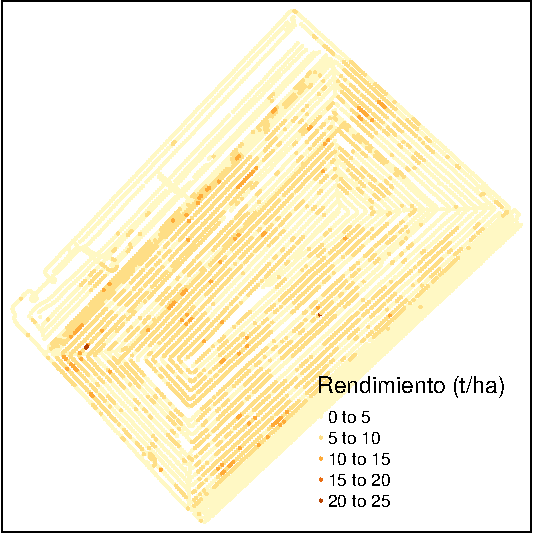
\includegraphics[width=\linewidth]{figuras/figLibro/unnamed-chunk-18-1} \end{center}

\hypertarget{eliminaciuxf3n-de-outliers-e-inliers}{%
\section{\texorpdfstring{Eliminación de \emph{outliers} e \emph{inliers}}{Eliminación de outliers e inliers}}\label{eliminaciuxf3n-de-outliers-e-inliers}}

En un \texttt{data.frame}, una forma sencilla para obtener medidas resumen de una variable es con la función \texttt{summary()}. Se utiliza \texttt{\$} para hacer referencia a una columna particular dentro de un objeto.

\begin{Shaded}
\begin{Highlighting}[]
\KeywordTok{summary}\NormalTok{(datos_sf}\OperatorTok{$}\NormalTok{Rinde)}
\CommentTok{#> Min. 1st Qu.  Median Mean 3rd Qu.  Max.}
\CommentTok{#> 0,00 3,71 4,68 4,62 5,48 24,00}
\end{Highlighting}
\end{Shaded}

Las funciones \texttt{hist()} y \texttt{boxplot()} realizan gráficos de histogramas y box-plots, respectivamente. Sus múltiples argumentos permiten la edición de cada gráfico. La función \texttt{par()} permite dividir la ventana gráfica de R, en el siguiente ejemplo se divide la ventana gráfica de R en dos columnas y una fila.

\begin{Shaded}
\begin{Highlighting}[]
\KeywordTok{par}\NormalTok{(}\DataTypeTok{mfrow =} \KeywordTok{c}\NormalTok{(}\DecValTok{1}\NormalTok{, }\DecValTok{2}\NormalTok{))}
\KeywordTok{hist}\NormalTok{(}
\NormalTok{  datos_sf}\OperatorTok{$}\NormalTok{Rinde,}
  \DataTypeTok{col =} \StringTok{'grey'}\NormalTok{,}
  \DataTypeTok{nclass =} \DecValTok{20}\NormalTok{,}
  \DataTypeTok{main =} \StringTok{"Histograma"}\NormalTok{,}
  \DataTypeTok{ylab =} \StringTok{'Frecuencia Relativa'}\NormalTok{,}
  \DataTypeTok{xlab =} \StringTok{'Rendimiento (t/ha)'}
\NormalTok{)}

\KeywordTok{boxplot}\NormalTok{(}
\NormalTok{  datos}\OperatorTok{$}\NormalTok{Rinde,}
  \DataTypeTok{col =} \StringTok{'grey'}\NormalTok{,}
  \DataTypeTok{ylab =} \StringTok{'Rendimiento (t/ha)'}\NormalTok{,}
  \DataTypeTok{main =} \StringTok{"Box-Plot"}\NormalTok{,}
  \DataTypeTok{ylim =} \KeywordTok{c}\NormalTok{(}\DecValTok{0}\NormalTok{, }\DecValTok{14}\NormalTok{)}
\NormalTok{)}
\end{Highlighting}
\end{Shaded}

\begin{center}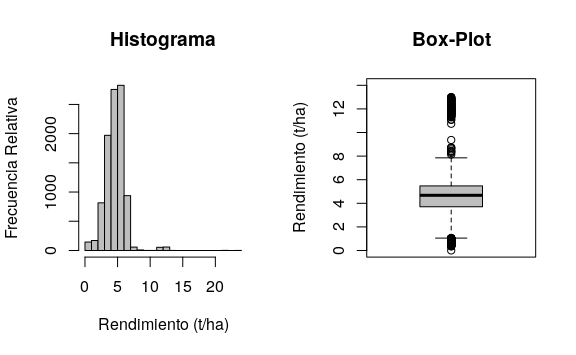
\includegraphics[width=\linewidth]{figuras/figLibro/fighistBox-1} \end{center}

a función \texttt{skewness()} del paquete \texttt{e1071} permite calcular el coeficiente de asimetría. Existen 3 fórmulas para su cálculo (por defecto usa el tipo 3). Para más información, se puede utilizar \texttt{help(skewness)}.

\begin{Shaded}
\begin{Highlighting}[]
\KeywordTok{skewness}\NormalTok{(datos_sf}\OperatorTok{$}\NormalTok{Rinde)}
\CommentTok{#> [1] 1,45}
\end{Highlighting}
\end{Shaded}

En el histograma se observa asimetría derecha en la distribución de los datos. La asimetría también puede advertirse con los estadísticos con el coeficiente de asimetría el cual es de 1,45. En el gráfico box-plot se observan valores extremos de la variable que se encuentran principalmente por encima de la media \(+\) 3 SD.

Las siguientes instrucciones calculan y crean objetos para la media, el DE y los límites superior (\(media + 3DE\)) e inferior (\(media - 3DE\)) con los que pueden detectarse los \emph{outliers} y elimina estos valores.

\begin{Shaded}
\begin{Highlighting}[]
\NormalTok{Media <-}\StringTok{ }\KeywordTok{mean}\NormalTok{(datos_sf}\OperatorTok{$}\NormalTok{Rinde)}
\NormalTok{DE <-}\StringTok{ }\KeywordTok{sd}\NormalTok{(datos_sf}\OperatorTok{$}\NormalTok{Rinde)}
\NormalTok{LI <-}\StringTok{ }\NormalTok{Media}\DecValTok{-3}\OperatorTok{*}\NormalTok{DE}
\NormalTok{LS <-}\StringTok{ }\NormalTok{Media}\OperatorTok{+}\DecValTok{3}\OperatorTok{*}\NormalTok{DE}
\end{Highlighting}
\end{Shaded}

Los símbolos \texttt{\textbar{}} y \texttt{\&} son operadores lógicos que significan \emph{or} y \emph{and}, respectivamente. Las siguientes instrucciones generan dos objetos. El objeto \texttt{datos\_1} es la base depurada, es decir sin \emph{outliers}, mientras que el objeto \texttt{outliers} presenta los datos que han sido eliminados en esta etapa.

\begin{Shaded}
\begin{Highlighting}[]
\NormalTok{datos_}\DecValTok{1}\NormalTok{ <-}
\StringTok{  }\KeywordTok{subset}\NormalTok{(datos_sf, }
\NormalTok{         datos_sf}\OperatorTok{$}\NormalTok{Rinde }\OperatorTok{<}\StringTok{ }\NormalTok{LS }\OperatorTok{&}\StringTok{ }
\StringTok{           }\NormalTok{datos_sf}\OperatorTok{$}\NormalTok{Rinde }\OperatorTok{>}\StringTok{ }\NormalTok{LI)}
\NormalTok{outliers <-}
\StringTok{  }\KeywordTok{subset}\NormalTok{(datos_sf, }
\NormalTok{         datos_sf}\OperatorTok{$}\NormalTok{Rinde }\OperatorTok{>}\StringTok{ }\NormalTok{LS }\OperatorTok{|}\StringTok{ }
\StringTok{           }\NormalTok{datos_sf}\OperatorTok{$}\NormalTok{Rinde }\OperatorTok{<}\StringTok{ }\NormalTok{LI)}
\end{Highlighting}
\end{Shaded}

Para ver el impacto de la eliminación de \emph{outliers} pueden obtenerse nuevamente las medidas resumen, coeficiente de asimetría, histograma y box-plot.

\begin{Shaded}
\begin{Highlighting}[]
\KeywordTok{summary}\NormalTok{(datos_}\DecValTok{1}\OperatorTok{$}\NormalTok{Rinde)}
\CommentTok{#> Min. 1st Qu.  Median Mean 3rd Qu.  Max.}
\CommentTok{#> 0,35 3,69 4,66 4,52 5,45 8,73}
\KeywordTok{skewness}\NormalTok{(datos_}\DecValTok{1}\OperatorTok{$}\NormalTok{Rinde)}
\CommentTok{#> [1] -0,536}
\end{Highlighting}
\end{Shaded}

\begin{Shaded}
\begin{Highlighting}[]
\KeywordTok{par}\NormalTok{(}\DataTypeTok{mfrow =} \KeywordTok{c}\NormalTok{(}\DecValTok{1}\NormalTok{, }\DecValTok{2}\NormalTok{))}
\KeywordTok{hist}\NormalTok{(}
\NormalTok{  datos_}\DecValTok{1}\OperatorTok{$}\NormalTok{Rinde,}
  \DataTypeTok{col =} \StringTok{'grey'}\NormalTok{,}
  \DataTypeTok{nclass =} \DecValTok{20}\NormalTok{,}
  \DataTypeTok{main =} \StringTok{"Histograma"}\NormalTok{,}
  \DataTypeTok{ylab =} \StringTok{'Frecuencia Relativa'}\NormalTok{,}
  \DataTypeTok{xlab =} \StringTok{'Rinde (t/ha)'}
\NormalTok{)}
\KeywordTok{boxplot}\NormalTok{(}
\NormalTok{  datos_}\DecValTok{1}\OperatorTok{$}\NormalTok{Rinde,}
  \DataTypeTok{col =} \StringTok{'grey'}\NormalTok{,}
  \DataTypeTok{ylab =} \StringTok{'Rinde (t/ha)'}\NormalTok{,}
  \DataTypeTok{main =} \StringTok{"Box-Plot"}\NormalTok{,}
  \DataTypeTok{ylim =} \KeywordTok{c}\NormalTok{(}\DecValTok{0}\NormalTok{, }\DecValTok{14}\NormalTok{)}
\NormalTok{)}
\end{Highlighting}
\end{Shaded}

\begin{center}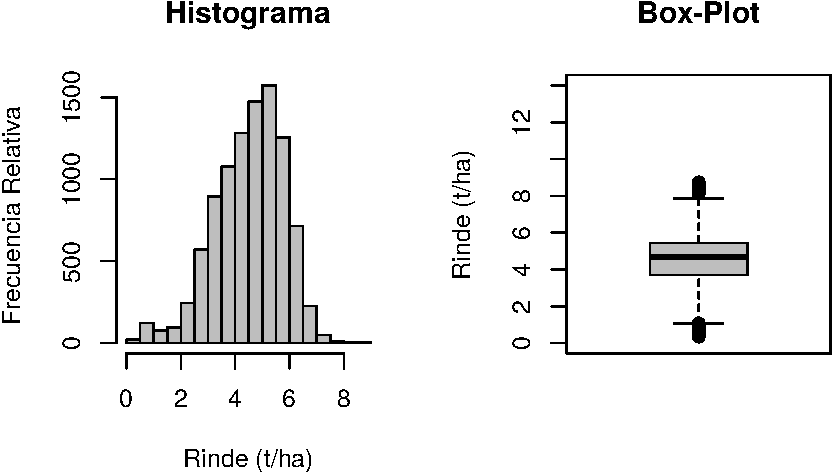
\includegraphics[width=\linewidth]{figuras/figLibro/unnamed-chunk-25-1} \end{center}

Las medidas resumen muestran un cambio principalmente a nivel de los valores máximos, pasando de 24 a 8,734 \(t\ ha^{-1}\). El coeficiente de asimetría presenta un valor de -0,54 que se aproxima a valores recomendados para el análisis geoestadístico (-1 a 1). En la figura anterior se presenta el histograma y box-plot luego de la eliminación de los \emph{outliers}. Para la variable en análisis, se eliminaron durante la depuración 120 casos que representan un 1,2\% del total de sitios (n=9810) con mediciones. Puede observarse una mejora en la simetría de la distribución de la variable y una marcada disminución de valores extremos.

La identificación y eliminación de \emph{inliers} requiere de la creación de una matriz de ponderación espacial. La función \texttt{dnearneigh()} se utiliza para identificar el vecindario de cada sitio. Para ello es necesario calcular la distancia espacial entre los puntos para lo cual se usa la sintaxis \texttt{\$geom} que permite acceder a las coordenadas del objeto \texttt{datos}. En este ejemplo, se consideran datos vecinos a aquellos que se encuentran a una distancia Euclídea de 0 a 15 m. La función \texttt{nb2listw()} transforma el objeto \texttt{vecindarios} que contiene las distancias a una matriz de pesos estandarizados por filas (\texttt{style\ =\ "W"}). Este objeto es denominado \texttt{pesos\_sp}. Para generar la matriz de pesos espaciales es necesario que todos los puntos tengan al menos un vecino, caso contario la función \texttt{nb2listw()} genera un error advirtiendo este hecho. Para superar el inconveniente es posible probar con distancias mayores hasta lograr que todos los puntos tengan al menos un vecino. Hay que tener la precaución de no generar un excesivo solapamiento entre los vecindarios. Otra opción es incorporar el argumento \texttt{zero.policy=T} dentro de la función \texttt{nb2listw()} que permite generar la matriz de pesos espaciales con observaciones que no presentan dato/s vecino/s. El mismo argumento debe agregarse luego cuando se calcula el índice de Moran local o gráfico de Moran (funciones \texttt{localmoran()} y \texttt{moran.plot()}, respectivamente). Las frecuencias del número de puntos vecinos para cada observación puede obtenerse mediante la función \texttt{summary()} del objeto \texttt{vecindarios}. En el ejemplo se observa que 3113 puntos tienen vecindarios conformados con 4 datos. Mientras que sólo un dato presenta 18 observaciones consideradas como vecinas.

\begin{Shaded}
\begin{Highlighting}[]
\NormalTok{vecindarios <-}\StringTok{ }\KeywordTok{dnearneigh}\NormalTok{(datos_}\DecValTok{1}\OperatorTok{$}\NormalTok{geom,}
                          \DataTypeTok{d1 =} \DecValTok{0}\NormalTok{, }\DataTypeTok{d2 =} \DecValTok{15}\NormalTok{)}
\KeywordTok{summary}\NormalTok{(vecindarios)}
\CommentTok{#> Neighbour list object:}
\CommentTok{#> Number of regions: 9690}
\CommentTok{#> Number of nonzero links: 62578}
\CommentTok{#> Percentage nonzero weights: 0,0666}
\CommentTok{#> Average number of links: 6,46}
\CommentTok{#> Link number distribution:}
\CommentTok{#>}
\CommentTok{#> 1 2 3 4 5 6 7 8 9 10 11 12 13 14 15 16}
\CommentTok{#> 5 83 302 3113 1292 999 893 870 393 457 547}
\DecValTok{473} \DecValTok{171} \DecValTok{43} \DecValTok{31} \DecValTok{13}
\CommentTok{#> [ reached getOption("max.print") -- omitted}
\DecValTok{2}\NormalTok{ entries ]}
\CommentTok{#> 5 least connected regions:}
\CommentTok{#> 3033 7885 9153 9598 9681 with 1 link}
\CommentTok{#> 1 most connected region:}
\CommentTok{#> 869 with 18 links}
\end{Highlighting}
\end{Shaded}

\begin{Shaded}
\begin{Highlighting}[]
\NormalTok{pesos_sp <-}\StringTok{ }\KeywordTok{nb2listw}\NormalTok{(vecindarios,}
                     \DataTypeTok{style =} \StringTok{"W"}\NormalTok{)}
\end{Highlighting}
\end{Shaded}

La función \texttt{localmoran()} calcula el índice local de Moran que permite identificar potenciales \emph{outliers} espaciales. También permite el ajuste de los \emph{valores-p} por el criterio de Bonferroni. La información referida al valor del índice local de Moran de cada punto se encuentra en la columna \texttt{Ii} mientras que su significancia estadística en la columna \texttt{Pr(z\ \textless{}\ 0)}.

\begin{Shaded}
\begin{Highlighting}[]
\NormalTok{moranl <-}
\StringTok{  }\KeywordTok{localmoran}\NormalTok{(datos_}\DecValTok{1}\OperatorTok{$}\NormalTok{Rinde,}
\NormalTok{             pesos_sp,}
             \DataTypeTok{p.adjust.method =} \StringTok{"bonferroni"}\NormalTok{,}
             \DataTypeTok{alternative =} \StringTok{"less"}\NormalTok{)}
\KeywordTok{head}\NormalTok{(moranl)}
\CommentTok{#> Ii E.Ii Var.Ii Z.Ii Pr(z < 0)}
\CommentTok{#> 1 5,32 -0,000103 0,0832 18,44 1}
\CommentTok{#> 2 6,83 -0,000103 0,1110 20,49 1}
\CommentTok{#> 3 5,83 -0,000103 0,0832 20,21 1}
\CommentTok{#> [ reached getOption("max.print") -- omitted}
\DecValTok{3}\NormalTok{ rows ]}
\end{Highlighting}
\end{Shaded}

El gráfico de Moran permite la identificación de puntos influyentes. La función \texttt{moran.plot()} construye el gráfico y devuelve los estadísticos de diagnóstico para cada punto. En el eje horizontal se expresan los valores de la variable rendimiento mientras que en el vertical se representa el retardo espacial de la variable. Adicionalmente, se ajusta y añade a este diagrama modelos de regresión lineal y estadísticos de influencia para identificar sitios con datos raros. Un punto se determina como influyente si al menos uno de los estadísticos así lo considera. En la figura siguiente los puntos negros con forma romboidal fueron identificados como influyentes y se los considera como \emph{inliers}.

\begin{Shaded}
\begin{Highlighting}[]
\NormalTok{moranp <-}
\StringTok{  }\KeywordTok{moran.plot}\NormalTok{(}
\NormalTok{    datos_}\DecValTok{1}\OperatorTok{$}\NormalTok{Rinde,}
    \DataTypeTok{col =} \DecValTok{3}\NormalTok{,}
\NormalTok{    pesos_sp,}
    \DataTypeTok{labels =}\NormalTok{ F,}
    \DataTypeTok{quiet =}\NormalTok{ T,}
    \DataTypeTok{xlab =} \StringTok{"Rinde"}\NormalTok{,}
    \DataTypeTok{ylab =} \StringTok{"Rinde Spatially Lagged"}
\NormalTok{  )}
\end{Highlighting}
\end{Shaded}

\begin{center}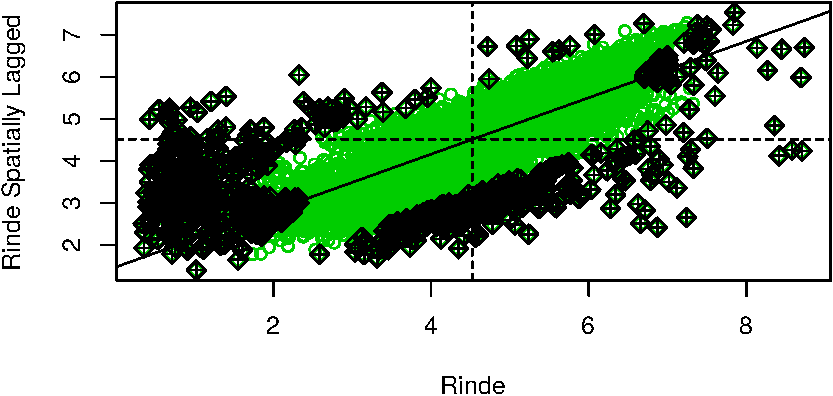
\includegraphics[width=\linewidth]{figuras/figLibro/unnamed-chunk-29-1} \end{center}

Para visualizar en una tabla los puntos potencialmente influyentes y sus estadísticos de diagnóstico puede imprimir el objeto \texttt{moranp}. Datos con * en la columna inf se los considera como influyente y por lo tanto posible \emph{outlier} espacial.

\begin{Shaded}
\begin{Highlighting}[]
\KeywordTok{summary}\NormalTok{(moranp)}
\end{Highlighting}
\end{Shaded}

Desde el objeto \texttt{moranp} puede extraerse una matriz de valores lógicos (verdadero/falso) para los estadísticos diagnóstico que identifican un punto como influyente o no.

\begin{Shaded}
\begin{Highlighting}[]
\NormalTok{influ <-}\StringTok{ }\NormalTok{moranp}\OperatorTok{$}\NormalTok{is.inf}
\KeywordTok{head}\NormalTok{(influ)}
\CommentTok{#> dfb.1_ dfb.x dffit cov.r cook.d hat}
\CommentTok{#> 1 FALSE FALSE TRUE TRUE FALSE TRUE}
\CommentTok{#> 2 FALSE FALSE FALSE TRUE FALSE TRUE}
\CommentTok{#> [ reached getOption("max.print") -- omitted}
\DecValTok{4}\NormalTok{ rows ]}
\end{Highlighting}
\end{Shaded}

En la siguiente sentencia se adiciona al objeto \texttt{datos\_1} los valores de los objetos \texttt{moranl} e \texttt{influ}, que tienen información para detectar los \emph{outliers} espaciales detectados con el índice de Moran local y gráfico de Moran, respectivamente.

\begin{Shaded}
\begin{Highlighting}[]
\NormalTok{datos_}\DecValTok{1}\NormalTok{ <-}\StringTok{ }\KeywordTok{cbind}\NormalTok{(datos_}\DecValTok{1}\NormalTok{, moranl, influ)}
\end{Highlighting}
\end{Shaded}

Posteriormente procedemos a eliminar los datos con Índice de Moran Local negativo y estadísticamente significativos (p\textless{}0,05). La función \texttt{subset()} selecciona datos que cumplen con cierta condición lógica. El operador lógico \emph{or} que indica que extraiga los datos que cumplen con alguna de las dos condiciones. El nuevo objeto es denominado \texttt{datos\_2}. Además, se crea un nuevo objeto que tendrá los datos que han sido eliminados en este proceso (\texttt{inliers\_ml}).

\begin{Shaded}
\begin{Highlighting}[]
\NormalTok{datos_}\DecValTok{2}\NormalTok{ <-}
\StringTok{  }\KeywordTok{subset}\NormalTok{(datos_}\DecValTok{1}\NormalTok{, }
\NormalTok{         datos_}\DecValTok{1}\NormalTok{[[}\StringTok{"Ii"}\NormalTok{]] }\OperatorTok{>=}\StringTok{ }\DecValTok{0} \OperatorTok{|}\StringTok{ }
\StringTok{           }\NormalTok{datos_}\DecValTok{1}\NormalTok{[[}\StringTok{"Pr.z...0."}\NormalTok{]] }\OperatorTok{>}\StringTok{ }\FloatTok{0.05}\NormalTok{)}
\NormalTok{inliers_ml <-}
\StringTok{  }\KeywordTok{subset}\NormalTok{(datos_}\DecValTok{1}\NormalTok{, }
\NormalTok{         datos_}\DecValTok{1}\NormalTok{[[}\StringTok{"Ii"}\NormalTok{]] }\OperatorTok{<}\StringTok{ }\DecValTok{0} \OperatorTok{&}
\StringTok{           }\NormalTok{datos_}\DecValTok{1}\NormalTok{[[}\StringTok{"Pr.z...0."}\NormalTok{]] }\OperatorTok{<}\StringTok{ }\FloatTok{0.05}\NormalTok{)}
\end{Highlighting}
\end{Shaded}

Existen varias formas de eliminar las filas de la tabla que fueron identificadas como \emph{inliers} con la función \texttt{moran.plot()}. Una alternativa es usando sentencias lógicas con los operadores \texttt{==} y \texttt{\&} que significan igualdad lógica y \emph{and} respectivamente. Como en el caso anterior se genera una nueva base (\texttt{datos\_3}) la cual no tendrá los datos considerados como \emph{outliers} y \emph{outliers} espaciales. También se genera una nueva base que tendrá solo los datos considerados aquí como \emph{outliers} espaciales (\texttt{inliers\_mp}).

\begin{Shaded}
\begin{Highlighting}[]
\NormalTok{datos_}\DecValTok{3}\NormalTok{ <-}
\StringTok{  }\NormalTok{datos_}\DecValTok{2}\NormalTok{[datos_}\DecValTok{2}\OperatorTok{$}\NormalTok{dfb}\FloatTok{.1}\NormalTok{_ }\OperatorTok{==}\StringTok{ }\OtherTok{FALSE} \OperatorTok{&}
\StringTok{            }\NormalTok{datos_}\DecValTok{2}\OperatorTok{$}\NormalTok{dfb.x }\OperatorTok{==}\StringTok{ }\OtherTok{FALSE} \OperatorTok{&}\StringTok{ }
\StringTok{            }\NormalTok{datos_}\DecValTok{2}\OperatorTok{$}\NormalTok{dffit }\OperatorTok{==}\StringTok{ }\OtherTok{FALSE} \OperatorTok{&}
\StringTok{            }\NormalTok{datos_}\DecValTok{2}\OperatorTok{$}\NormalTok{cov.r }\OperatorTok{==}\StringTok{ }\OtherTok{FALSE} \OperatorTok{&}
\StringTok{            }\NormalTok{datos_}\DecValTok{2}\OperatorTok{$}\NormalTok{cook.d  }\OperatorTok{==}\StringTok{ }\OtherTok{FALSE} \OperatorTok{&}\StringTok{ }
\StringTok{            }\NormalTok{datos_}\DecValTok{2}\OperatorTok{$}\NormalTok{hat }\OperatorTok{==}\StringTok{ }\OtherTok{FALSE}\NormalTok{, ]}
\end{Highlighting}
\end{Shaded}

La sentencia anterior instruye al software para que cree un objeto llamado \texttt{datos\_3} a partir de las filas del objeto \texttt{datos\_2} cuyas columnas \texttt{dfb.1}, \texttt{dfb.x}, \texttt{dffit}, \texttt{cov.r}, \texttt{cook.d} y \texttt{hat} son simultáneamente iguales a \texttt{FALSE}.

\begin{Shaded}
\begin{Highlighting}[]
\NormalTok{inliers_mp <-}
\StringTok{  }\NormalTok{datos_}\DecValTok{2}\NormalTok{[datos_}\DecValTok{2}\OperatorTok{$}\NormalTok{dfb}\FloatTok{.1}\NormalTok{_ }\OperatorTok{!=}\StringTok{ }\OtherTok{FALSE} \OperatorTok{|}
\StringTok{            }\NormalTok{datos_}\DecValTok{2}\OperatorTok{$}\NormalTok{dfb.x }\OperatorTok{!=}\StringTok{ }\OtherTok{FALSE} \OperatorTok{|}
\StringTok{            }\NormalTok{datos_}\DecValTok{2}\OperatorTok{$}\NormalTok{dffit }\OperatorTok{!=}\StringTok{ }\OtherTok{FALSE} \OperatorTok{|}
\StringTok{            }\NormalTok{datos_}\DecValTok{2}\OperatorTok{$}\NormalTok{cov.r }\OperatorTok{!=}\StringTok{ }\OtherTok{FALSE} \OperatorTok{|}
\StringTok{            }\NormalTok{datos_}\DecValTok{2}\OperatorTok{$}\NormalTok{cook.d  }\OperatorTok{!=}\StringTok{ }\OtherTok{FALSE} \OperatorTok{|}\StringTok{ }
\StringTok{            }\NormalTok{datos_}\DecValTok{2}\OperatorTok{$}\NormalTok{hat }\OperatorTok{!=}\StringTok{ }\OtherTok{FALSE}\NormalTok{, ]}
\end{Highlighting}
\end{Shaded}

Luego de identificar y eliminar los \emph{inliers} detectados con el índice de Moran y posteriormente con el gráfico de Moran, la nueva base de datos presenta 9009 casos, es decir, se eliminaron 681 casos (7\% de los datos) respecto a la base sin \emph{outliers}.

Los estadísticos descriptivos de los datos depurados muestran una mejora en el coeficiente de asimetría (-0,19) lo cual se refleja en el histograma y box-plot. Este último también muestra la ausencia de valores extremos.

\begin{Shaded}
\begin{Highlighting}[]
\KeywordTok{summary}\NormalTok{(datos_}\DecValTok{3}\OperatorTok{$}\NormalTok{Rinde)}
\CommentTok{#> Min. 1st Qu.  Median Mean 3rd Qu.  Max.}
\CommentTok{#> 1,73 3,81 4,72 4,63 5,46 7,32}
\KeywordTok{skewness}\NormalTok{(datos_}\DecValTok{3}\OperatorTok{$}\NormalTok{Rinde)}
\CommentTok{#> [1] -0,197}
\end{Highlighting}
\end{Shaded}

\begin{Shaded}
\begin{Highlighting}[]
\KeywordTok{par}\NormalTok{(}\DataTypeTok{mfrow =} \KeywordTok{c}\NormalTok{(}\DecValTok{1}\NormalTok{, }\DecValTok{2}\NormalTok{))}
\KeywordTok{hist}\NormalTok{(}
\NormalTok{  datos_}\DecValTok{3}\OperatorTok{$}\NormalTok{Rinde,}
  \DataTypeTok{col =} \StringTok{'grey'}\NormalTok{,}
  \DataTypeTok{nclass =} \DecValTok{20}\NormalTok{,}
  \DataTypeTok{main =} \StringTok{"Histograma"}\NormalTok{,}
  \DataTypeTok{ylab =} \StringTok{'Frecuencia Relativa'}\NormalTok{,}
  \DataTypeTok{xlab =} \StringTok{'Rendimiento (t/ha)'}
\NormalTok{)}
\KeywordTok{boxplot}\NormalTok{(}
\NormalTok{  datos_}\DecValTok{3}\OperatorTok{$}\NormalTok{Rinde,}
  \DataTypeTok{col =} \StringTok{'grey'}\NormalTok{,}
  \DataTypeTok{ylab =} \StringTok{'Rendimiento (t/ha)'}\NormalTok{,}
  \DataTypeTok{main =} \StringTok{"Box-Plot"}\NormalTok{,}
  \DataTypeTok{ylim =} \KeywordTok{c}\NormalTok{(}\DecValTok{0}\NormalTok{, }\DecValTok{14}\NormalTok{)}
\NormalTok{)}
\end{Highlighting}
\end{Shaded}

\begin{center}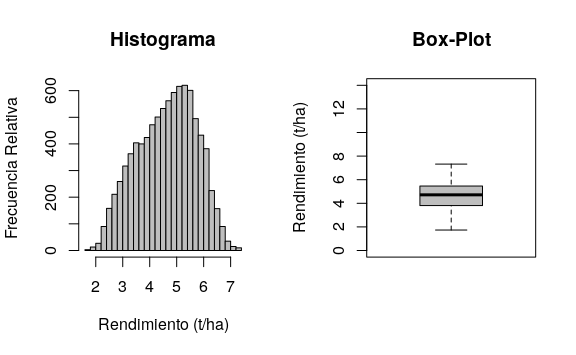
\includegraphics[width=\linewidth]{figuras/figLibro/unnamed-chunk-39-1} \end{center}

Las siguientes líneas muestran la visualización conjunta de los datos originales y aquellos detectados como \emph{outliers} y \emph{outliers} espaciales. En este último se diferencian los detectados por el índice de Moran local (\emph{Inliers} ML) respecto a los identificados por el gráfico de Moran (\emph{Inliers} MP).

\begin{Shaded}
\begin{Highlighting}[]

\KeywordTok{tmap_mode}\NormalTok{(}\StringTok{"plot"}\NormalTok{)}
\CommentTok{#> tmap mode set to plotting}
\KeywordTok{tm_shape}\NormalTok{(datos_}\DecValTok{3}\NormalTok{) }\OperatorTok{+}
\StringTok{  }\KeywordTok{tm_dots}\NormalTok{(}\StringTok{"Rinde"}\NormalTok{, }\DataTypeTok{title=}\StringTok{"Rendimiento (t/ha)"}\NormalTok{) }\OperatorTok{+}
\StringTok{  }\KeywordTok{tm_shape}\NormalTok{(outliers) }\OperatorTok{+}
\StringTok{  }\KeywordTok{tm_dots}\NormalTok{(}\DataTypeTok{col =} \StringTok{"red"}\NormalTok{, }\DataTypeTok{size =} \FloatTok{0.1}\NormalTok{) }\OperatorTok{+}
\StringTok{  }\KeywordTok{tm_shape}\NormalTok{(inliers_ml) }\OperatorTok{+}
\StringTok{  }\KeywordTok{tm_dots}\NormalTok{(}\DataTypeTok{col =} \StringTok{"blue"}\NormalTok{, }\DataTypeTok{size =} \FloatTok{0.1}\NormalTok{) }\OperatorTok{+}
\StringTok{  }\KeywordTok{tm_shape}\NormalTok{(inliers_mp) }\OperatorTok{+}
\StringTok{  }\KeywordTok{tm_dots}\NormalTok{(}\StringTok{"cyan"}\NormalTok{, }\DataTypeTok{size =} \FloatTok{0.1}\NormalTok{) }\OperatorTok{+}
\StringTok{  }\KeywordTok{tm_add_legend}\NormalTok{(}\StringTok{"symbol"}\NormalTok{, }
                \DataTypeTok{col =} \KeywordTok{c}\NormalTok{(}\StringTok{"red"}\NormalTok{, }\StringTok{"blue"}\NormalTok{, }\StringTok{"cyan"}\NormalTok{), }
                \DataTypeTok{labels =} \KeywordTok{c}\NormalTok{(}\StringTok{"Outliers"}\NormalTok{, }
                           \StringTok{"Inliers ML"}\NormalTok{, }
                           \StringTok{"Inliers MP"}\NormalTok{))}
\end{Highlighting}
\end{Shaded}

\begin{center}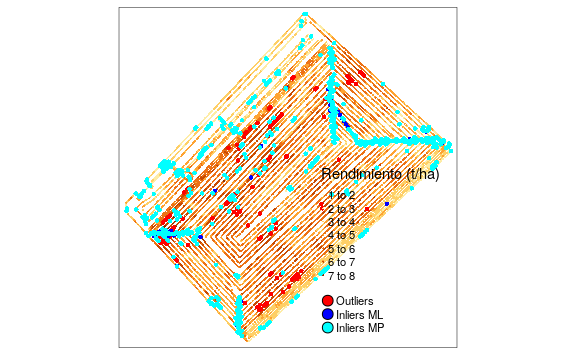
\includegraphics[width=\linewidth]{figuras/figLibro/tmapvarios-1} \end{center}

Finalmente las líneas siguientes permiten la exportación de los datos depurados en diferentes formatos (.csv, .shp, .gpkg). para ello se utiliza la función \texttt{st\_write()}. Previo a ello se selecciona solo la variable Rinde del objeto \texttt{datos\_3}.

\begin{Shaded}
\begin{Highlighting}[]
\NormalTok{datos_}\DecValTok{3}\NormalTok{ <-}\StringTok{ }\NormalTok{datos_}\DecValTok{3}\NormalTok{[, }\KeywordTok{c}\NormalTok{(}\StringTok{"Rinde"}\NormalTok{)]}
\KeywordTok{st_write}\NormalTok{(datos_}\DecValTok{3}\NormalTok{,}
         \StringTok{"base_depurada.csv"}\NormalTok{,}
         \DataTypeTok{layer_options =} \StringTok{"GEOMETRY=AS_XY"}\NormalTok{,}
         \DataTypeTok{delete_layer =}\NormalTok{ T)}
\KeywordTok{st_write}\NormalTok{(datos_}\DecValTok{3}\NormalTok{, }
         \StringTok{"base_depurada.shp"}\NormalTok{, }
         \DataTypeTok{delete_layer =}\NormalTok{ T)}
\KeywordTok{st_write}\NormalTok{(datos_}\DecValTok{3}\NormalTok{, }
         \StringTok{"base_depurada.gpkg"}\NormalTok{, }
         \DataTypeTok{delete_layer =}\NormalTok{ T)}
\end{Highlighting}
\end{Shaded}

\hypertarget{detecciuxf3n-de-tendencias-espaciales}{%
\section{Detección de tendencias espaciales}\label{detecciuxf3n-de-tendencias-espaciales}}

Para evaluar las tendencia de la media del rendimiento con las coordenadas geográficas primero se incorpora al \texttt{data.frame} del objeto \texttt{sf} las coordenadas. De esta forma el objeto \texttt{datos\_3} presenta la variable Rinde, su geometría y las coordenadas x e y.

\begin{Shaded}
\begin{Highlighting}[]
\NormalTok{datos_}\DecValTok{3}\OperatorTok{$}\NormalTok{x <-}\StringTok{ }\KeywordTok{st_coordinates}\NormalTok{(datos_}\DecValTok{3}\NormalTok{)[,}\DecValTok{1}\NormalTok{]}
\NormalTok{datos_}\DecValTok{3}\OperatorTok{$}\NormalTok{y <-}\StringTok{ }\KeywordTok{st_coordinates}\NormalTok{(datos_}\DecValTok{3}\NormalTok{)[,}\DecValTok{2}\NormalTok{]}
\KeywordTok{head}\NormalTok{(datos_}\DecValTok{3}\NormalTok{)}
\CommentTok{#> Simple feature collection with 6 features}
\NormalTok{and }\DecValTok{3}\NormalTok{ fields}
\CommentTok{#> geometry type: POINT}
\CommentTok{#> dimension: XY}
\CommentTok{#> bbox: xmin: 312000 ymin: 5800000 xmax:}
\DecValTok{313000}\NormalTok{ ymax}\OperatorTok{:}\StringTok{ }\DecValTok{5800000}
\CommentTok{#> epsg (SRID): 32721}
\CommentTok{#> proj4string: }
    \OperatorTok{+}\StringTok{ }\NormalTok{proj=utm }
    \OperatorTok{+}\StringTok{ }\NormalTok{zone=}\DecValTok{21} 
    \OperatorTok{+}\StringTok{ }\NormalTok{south}
\OperatorTok{+}\NormalTok{datum=WGS84 }\OperatorTok{+}\NormalTok{units=m }\OperatorTok{+}\NormalTok{no_defs}
\CommentTok{#> First 3 features:}
\CommentTok{#> Rinde geometry x y}
\CommentTok{#> 256 1,73 POINT (311987 5800811) 311987}
\DecValTok{5800811}
\CommentTok{#> 257 1,73 POINT (313167 5800905) 313167}
\DecValTok{5800905}
\CommentTok{#> 263 1,78 POINT (312511 5800721) 312511}
\DecValTok{5800721}
\end{Highlighting}
\end{Shaded}

Para visualizar tendencias espaciales graficamos la variable en estudio en función de las coordenadas. Si se desea desplegar los gráficos para la coordenada x e y en una misma ventana gráfica, se puede particionar la ventana en una fila y dos columnas utilizando la siguiente función:

\begin{Shaded}
\begin{Highlighting}[]
\KeywordTok{par}\NormalTok{(}\DataTypeTok{mfrow=}\KeywordTok{c}\NormalTok{(}\DecValTok{1}\NormalTok{,}\DecValTok{2}\NormalTok{))}
\end{Highlighting}
\end{Shaded}

La función \texttt{plot()} permite realizar gráficos de dispersión. Además, puede adicionarse una línea de suavizado \emph{lowess} con la función \texttt{lines()}. Esta última, realiza el ajuste sobre una ventana gráfica preexistente.

\begin{Shaded}
\begin{Highlighting}[]
\KeywordTok{par}\NormalTok{(}\DataTypeTok{mfrow =} \KeywordTok{c}\NormalTok{(}\DecValTok{1}\NormalTok{, }\DecValTok{2}\NormalTok{))}

\KeywordTok{with}\NormalTok{(datos_}\DecValTok{3}\NormalTok{, \{}
  \KeywordTok{plot}\NormalTok{(Rinde }\OperatorTok{~}\StringTok{ }\NormalTok{x)}
  \KeywordTok{lines}\NormalTok{(}\KeywordTok{lowess}\NormalTok{(Rinde }\OperatorTok{~}\StringTok{ }\NormalTok{x), }
        \DataTypeTok{col =} \StringTok{"red"}\NormalTok{, }\DataTypeTok{lwd =} \DecValTok{3}\NormalTok{)}

\NormalTok{\})}
\KeywordTok{with}\NormalTok{(datos_}\DecValTok{3}\NormalTok{, \{}
  \KeywordTok{plot}\NormalTok{(Rinde }\OperatorTok{~}\StringTok{ }\NormalTok{y)}
  \KeywordTok{lines}\NormalTok{(}\KeywordTok{lowess}\NormalTok{(Rinde }\OperatorTok{~}\StringTok{ }\NormalTok{y), }
        \DataTypeTok{col =} \StringTok{"red"}\NormalTok{, }\DataTypeTok{lwd =} \DecValTok{3}\NormalTok{) }
\NormalTok{\})}
\end{Highlighting}
\end{Shaded}

\begin{center}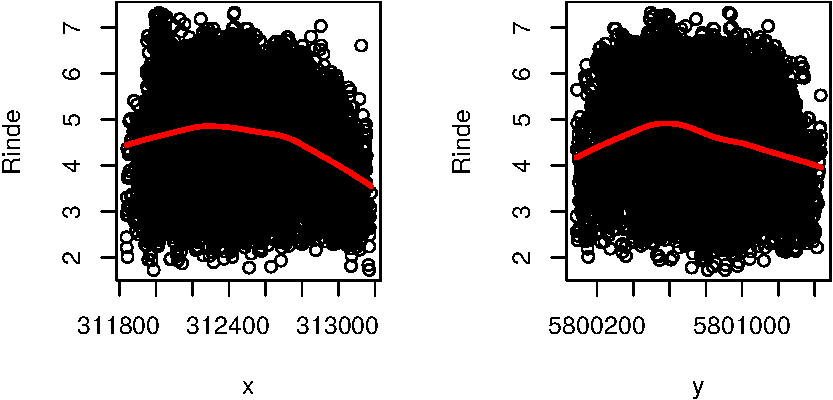
\includegraphics[width=\linewidth]{figuras/figLibro/unnamed-chunk-44-1} \end{center}

Mediante un modelo lineal de regresión, puede ajustarse la tendencia entre la variable en estudio y las coordenadas. Si la tendencia lineal resulta significativa, debería descontarse trabajando con los residuos del modelo, que se obtienen con la función \texttt{residuals()}.

\begin{Shaded}
\begin{Highlighting}[]
\NormalTok{regresion <-}\StringTok{ }\KeywordTok{lm}\NormalTok{(}\DataTypeTok{formula =}\NormalTok{ Rinde }\OperatorTok{~}\StringTok{ }\DecValTok{1} \OperatorTok{+}\StringTok{ }\NormalTok{x }\OperatorTok{+}\StringTok{ }\NormalTok{y ,}
                \DataTypeTok{data =}\NormalTok{ datos_}\DecValTok{3}\NormalTok{,}
                \DataTypeTok{na.action =}\NormalTok{ na.omit)}
\end{Highlighting}
\end{Shaded}

La siguiente línea despliega una tabla resumen del modelo:

\begin{Shaded}
\begin{Highlighting}[]
\KeywordTok{summary}\NormalTok{(regresion)}
\CommentTok{#>}
\CommentTok{#> Call:}
\CommentTok{#> lm(formula = Rinde ~ 1 + x + y, data =}
\NormalTok{datos_}\DecValTok{3}\NormalTok{, na.action =}\StringTok{ }\NormalTok{na.omit}\ErrorTok{)}
\CommentTok{#>}
\CommentTok{#> Residuals:}
\CommentTok{#> Min 1Q Median 3Q Max}
\CommentTok{#> -3,165 -0,811 0,102 0,819 2,736}
\CommentTok{#>}
\CommentTok{#> Coefficients:}
\CommentTok{#> Estimate Std. Error t value Pr(>|t|)}
\CommentTok{#> (Intercept) 1,84e+03 2,34e+02 7,85 4,6e-15}
\OperatorTok{**}\ErrorTok{*}
\CommentTok{#> x -5,56e-04 4,10e-05 -13,54 < 2e-16 ***}
\CommentTok{#> y -2,86e-04 4,10e-05 -6,98 3,2e-12 ***}
\CommentTok{#> ---}
\CommentTok{#> Signif. codes: 0 '***'}
\StringTok{    }\DecValTok{0}\NormalTok{,}\DecValTok{001} \StringTok{'**'}
    \DecValTok{0}\NormalTok{,}\DecValTok{01} \StringTok{'*'}
\DecValTok{0}\NormalTok{,}\DecValTok{05} \StringTok{'.'}
    \DecValTok{0}\NormalTok{,}\DecValTok{1} \StringTok{'}
\StringTok{    '}
    \DecValTok{1}
\CommentTok{#>}
\CommentTok{#> Residual standard error: 1,07 on 9006}
\NormalTok{degrees of freedom}
\CommentTok{#> Multiple R-squared: 0,0348, Adjusted}
\NormalTok{R}\OperatorTok{-}\NormalTok{squared}\OperatorTok{:}\StringTok{ }\DecValTok{0}\NormalTok{,}\DecValTok{0346}
\CommentTok{#> F-statistic: 162 on 2 and 9006 DF, p-value:}
\OperatorTok{<}\FloatTok{2e-16}
\end{Highlighting}
\end{Shaded}

En este caso, los gráficos exploratorios no marcan una tendencia marcada con las coordenadas. Aún, cuando los valores-p del modelo de regresión son significativos (p\textless{}0,05), se decidió trabajar con la variable original debido a que el coeficiente de determinación del modelo acusa un ajuste pobre (0,035).

\hypertarget{cuxe1lculo-del-uxedndice-de-moran}{%
\section{Cálculo del índice de Moran}\label{cuxe1lculo-del-uxedndice-de-moran}}

Para la conformación de la matriz de ponderadores espaciales se definieron los vecindarios de cada sitio mediante una red de conexión construida en base a la distancia euclídea. Se consideraron sitios vecinos a aquellos contiguos ubicados hasta 15 m de distancia. El procedimiento es similar al empleado para el cálculo de índice de Moran local. En este caso se agrega el argumento \texttt{zero.policy=T} dentro de la función \texttt{nb2listw()} y \texttt{moran.mc()}. Esto permite que se genera la matriz de pesos espaciales sin la restricción de que todos los puntos tengan al menos un dato vecino.

\begin{Shaded}
\begin{Highlighting}[]
\NormalTok{vecindarios <-}\StringTok{ }\KeywordTok{dnearneigh}\NormalTok{(datos_}\DecValTok{3}\OperatorTok{$}\NormalTok{geom, }
                          \DecValTok{0}\NormalTok{, }\DecValTok{15}\NormalTok{)}
\NormalTok{pesos_sp <-}\StringTok{ }\KeywordTok{nb2listw}\NormalTok{(vecindarios, }
                     \DataTypeTok{style =} \StringTok{"W"}\NormalTok{, }
                     \DataTypeTok{zero.policy =} \OtherTok{TRUE}\NormalTok{)}
\end{Highlighting}
\end{Shaded}

Para realizar el cálculo del Índice de Moran y determinar su significancia estadística mediante simulación Monte Carlo, se utiliza \texttt{moran.mc()}. Se debe especificar la variable en estudio, la lista con los pesos de las ponderaciones espaciales y el número de simulaciones.

\begin{Shaded}
\begin{Highlighting}[]
\NormalTok{i.moran <-}
\StringTok{  }\KeywordTok{moran.mc}\NormalTok{(}
\NormalTok{    datos_}\DecValTok{3}\OperatorTok{$}\NormalTok{Rinde,}
    \DataTypeTok{listw =}\NormalTok{ pesos_sp,}
    \DataTypeTok{nsim =} \DecValTok{999}\NormalTok{,}
    \DataTypeTok{zero.policy =}\NormalTok{ T}
\NormalTok{  )}
\NormalTok{i.moran}
\CommentTok{#>}
\CommentTok{#> Monte-Carlo simulation of Moran I}
\CommentTok{#>}
\CommentTok{#> data: datos_3$Rinde}
\CommentTok{#> weights: pesos_sp}
\CommentTok{#> number of simulations + 1: 1000}
\CommentTok{#>}
\CommentTok{#> statistic = 0,8, observed rank = 1000,}
\NormalTok{p}\OperatorTok{-}\NormalTok{value =}\StringTok{ }\DecValTok{0}\NormalTok{,}\DecValTok{001}
\CommentTok{#> alternative hypothesis: greater}
\end{Highlighting}
\end{Shaded}

Estos resultados permiten concluir que existe autocorrelación espacial positiva (0,78196) y que esta es estadísticamente significativa (p=0,001).

\hypertarget{anuxe1lisis-basado-en-semivariogramas}{%
\section{Análisis basado en semivariogramas}\label{anuxe1lisis-basado-en-semivariogramas}}

Las semivariogramas empíricos pueden obtenerse usando la función \texttt{variogram()} del paquete \texttt{gstat}. Esta tiene múltiples argumentos, entre ellos una fórmula, un objeto de datos espaciales y la distancia hasta la cual los pares de puntos son incluidos en la estimación de semivarianza (\texttt{cutoff}). Dado que el objeto a tratar (\texttt{datos\_3}) es de clase \texttt{sf}, no es necesario realizar su transformación a un objeto del tipo espacial. Utilizando la función plot() se visualiza el semivariograma empírico ajustado.

\begin{Shaded}
\begin{Highlighting}[]
\NormalTok{semiv_emp <-}\StringTok{ }\KeywordTok{variogram}\NormalTok{(Rinde }\OperatorTok{~}\StringTok{ }\DecValTok{1}\NormalTok{, }
\NormalTok{                       datos_}\DecValTok{3}\NormalTok{, }
                       \DataTypeTok{cutoff =} \DecValTok{400}\NormalTok{)}
\KeywordTok{head}\NormalTok{(semiv_emp)}
\CommentTok{#> np dist gamma dir.hor dir.ver id}
\CommentTok{#> 1 97403 18,0 0,412 0 0 var1}
\CommentTok{#> 2 281953 41,4 0,643 0 0 var1}
\CommentTok{#> [ reached 'max'}
    \OperatorTok{/}\StringTok{ }\KeywordTok{getOption}\NormalTok{(}\StringTok{"max.print"}\NormalTok{) }\OperatorTok{--}
\NormalTok{omitted }\DecValTok{4}\NormalTok{ rows ]}
\end{Highlighting}
\end{Shaded}

\begin{Shaded}
\begin{Highlighting}[]
\KeywordTok{plot}\NormalTok{(semiv_emp,}
     \DataTypeTok{main =} \StringTok{"Rendimiento (t/ha)"}\NormalTok{,}
     \DataTypeTok{xlab =} \StringTok{"Distancia"}\NormalTok{,}
     \DataTypeTok{ylab =} \StringTok{"Semivarianza"}\NormalTok{)}
\end{Highlighting}
\end{Shaded}

\begin{center}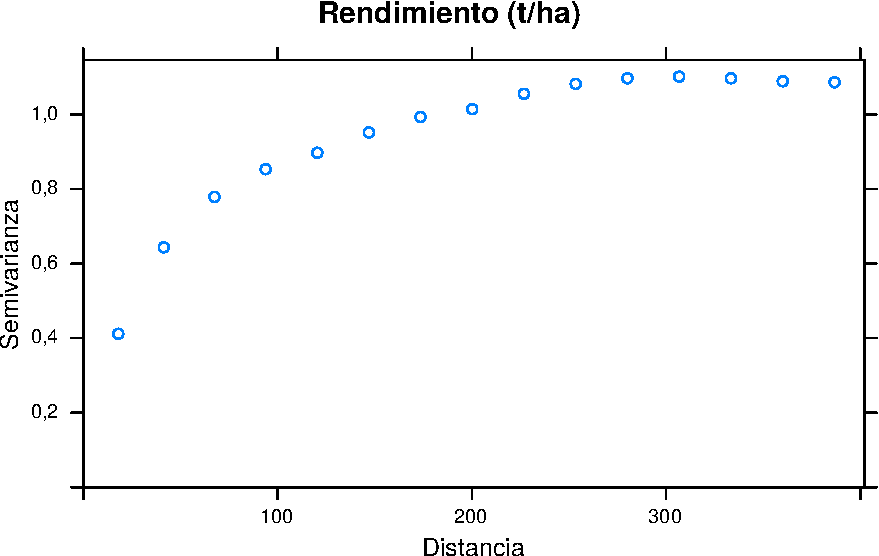
\includegraphics[width=\linewidth]{figuras/figLibro/unnamed-chunk-50-1} \end{center}

En el caso anterior la fórmula utilizada (\texttt{Rinde\textasciitilde{}1}) asume que el proceso es estacionario. Si se requiere adicionar una tendencia sea reemplaza el caracter 1 por el nombre de la covariable. Por ejemplo, si existe una tendencia dada por las coordenadas la fórmula se escribe como \texttt{Rinde\textasciitilde{}x+y}. Es posible solo colocar una de las coordenadas o incluir también términos polinómicos para las mismas. También se pueden usar otras covariables distintas a las coordenadas.

Por defecto para el cálculo del semivariograma empírico la función \texttt{variogram()} utiliza el estimador de los momentos de Matheron. Para emplear el estimador robusto de Cressie-Hawkins se adiciona en la función el argumento \texttt{cresice=TRUE}. Por defecto la función emplea para el cálculo del semivariograma un tercio de la diagonal del ``cuadro'' que contiene las observaciones. Con el argumento \texttt{cutoff} se puede cambiar esta distancia. El argumento \texttt{width} permite cambiar el ancho de los intervalos de distancia en los que se agrupan los pares de puntos de datos para las estimaciones de semivarianza. Por defecto se calcula como \texttt{cutoff/15}. El argumento alpha permite el cálculo de los semivariogramas en distintas direcciones en el plano (x, y), tomando valores en grados positivos en sentido horario desde y (Norte). Para \texttt{alpha\ =\ 0} la dirección es Norte y para \texttt{alpha\ =\ 90} la dirección es Este. Esto es útil para evaluar la presencia de anisotropía. Usualmente se suelen calcular los semivariogramas direccionales para \(45^\circ\), \(90^\circ\), \(135^\circ\) y \(180^\circ\). Otras opciones pueden encontrarse mediante la función \texttt{help()}.

A continuación se ajusta un modelo de semivariograma teórico sobre el semivariograma empírico usando las funciones \texttt{fit.variogram()} y\texttt{vgm()}. Esta última ajusta el modelo teórico, sus argumentos indican el tipo de modelo a ajustar y los parámetros de ajuste (\emph{partial sill}, rango y efecto \emph{nugget}). Estos parámetros iniciales son de referencia y pueden obtenerse a partir del semivariograma empírico. Cambiar los parámetros modifica la suma de cuadrados del error (SCE).

Se ajusta un modelo esférico, con valores 0,6, 200 y 0,2 como parámetros iniciales para estimar el \emph{sill} parcial, rango y \emph{nugget}, respectivamente. La salida del software R muestra los parámetros del semivariograma teórico ajustado: \emph{nugget} (\(C_0=0.31\)), sill parcial (\(C=0.72\)) y rango (154 m). Nota: bajo la columna \emph{psill}, para la fila Nug, se debe leer el valor \(C_0\).

\begin{Shaded}
\begin{Highlighting}[]
\NormalTok{mod_esf <-}\StringTok{ }\KeywordTok{fit.variogram}\NormalTok{(}
\NormalTok{  semiv_emp,}
  \KeywordTok{vgm}\NormalTok{(}\FloatTok{0.6}\NormalTok{, }\StringTok{"Sph"}\NormalTok{, }\DecValTok{200}\NormalTok{, }\FloatTok{0.2}\NormalTok{))}
\NormalTok{mod_esf}
\CommentTok{#>   model psill range}
\CommentTok{#> 1   Nug 0,309     0}
\CommentTok{#> 2   Sph 0,719   154}
\end{Highlighting}
\end{Shaded}

El semivariograma empírico (puntos) y teórico ajustado(linea), para un modelo esférico, puede graficarse de la siguiente manera:

\begin{Shaded}
\begin{Highlighting}[]
\KeywordTok{plot}\NormalTok{(semiv_emp,}
\NormalTok{     mod_esf,}
     \DataTypeTok{main =} \StringTok{"Rendimiento (t/ha)"}\NormalTok{,}
     \DataTypeTok{xlab =} \StringTok{"Distancia"}\NormalTok{,}
     \DataTypeTok{ylab =} \StringTok{"Semivarianza"}\NormalTok{)}
\end{Highlighting}
\end{Shaded}

\begin{center}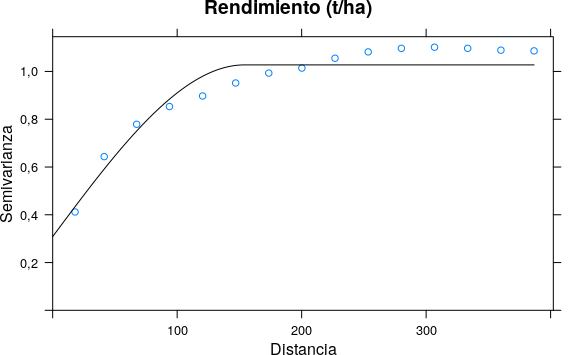
\includegraphics[width=\linewidth]{figuras/figLibro/unnamed-chunk-52-1} \end{center}

El modelo que mejor ajusta será el de menor SCE. La función \texttt{attr()} devuelve atributos de un objeto y puede usarse para consultar la SCE del modelo ajustado.

\begin{Shaded}
\begin{Highlighting}[]
\KeywordTok{attr}\NormalTok{(mod_esf, }\StringTok{'SSErr'}\NormalTok{)}
\CommentTok{#> [1] 1,7}
\end{Highlighting}
\end{Shaded}

Repitiendo el procedimiento para un modelo exponencial (especificado en la función \texttt{vgm()}) se obtiene un menor SCE indicando mejor ajuste. Abajo se presenta la salida del software R que contiene los parámetros del semivariograma teórico ajustado: nugget (\(C_0=0.21\)), sill parcial (\(C=0.86\)) y rango (64,88 m) o Rango Practico (\(Rp=64.88 m \times 3\)). Nota: bajo la columna ``psill'', para la fila Nugget, se debe leer el valor \(C_0\).

\begin{Shaded}
\begin{Highlighting}[]
\NormalTok{mod_exp <-}\StringTok{ }\KeywordTok{fit.variogram}\NormalTok{(}
\NormalTok{  semiv_emp, }
  \KeywordTok{vgm}\NormalTok{(}\FloatTok{0.6}\NormalTok{, }\StringTok{"Exp"}\NormalTok{, }\DecValTok{200}\NormalTok{, }\FloatTok{0.2}\NormalTok{))}
\NormalTok{mod_exp}
\CommentTok{#>   model psill range}
\CommentTok{#> 1   Nug 0,212   0,0}
\CommentTok{#> 2   Exp 0,860  64,9}
\end{Highlighting}
\end{Shaded}

\begin{Shaded}
\begin{Highlighting}[]
\KeywordTok{attr}\NormalTok{(mod_exp, }\StringTok{'SSErr'}\NormalTok{)}
\CommentTok{#> [1] 0,377}
\end{Highlighting}
\end{Shaded}

\begin{Shaded}
\begin{Highlighting}[]
\KeywordTok{plot}\NormalTok{(semiv_emp,}
\NormalTok{     mod_exp,}
     \DataTypeTok{main =} \StringTok{"Rendimiento (t/ha)"}\NormalTok{,}
     \DataTypeTok{xlab =} \StringTok{"Distancia"}\NormalTok{,}
     \DataTypeTok{ylab =} \StringTok{"Semivarianza"}\NormalTok{)}
\end{Highlighting}
\end{Shaded}

\begin{center}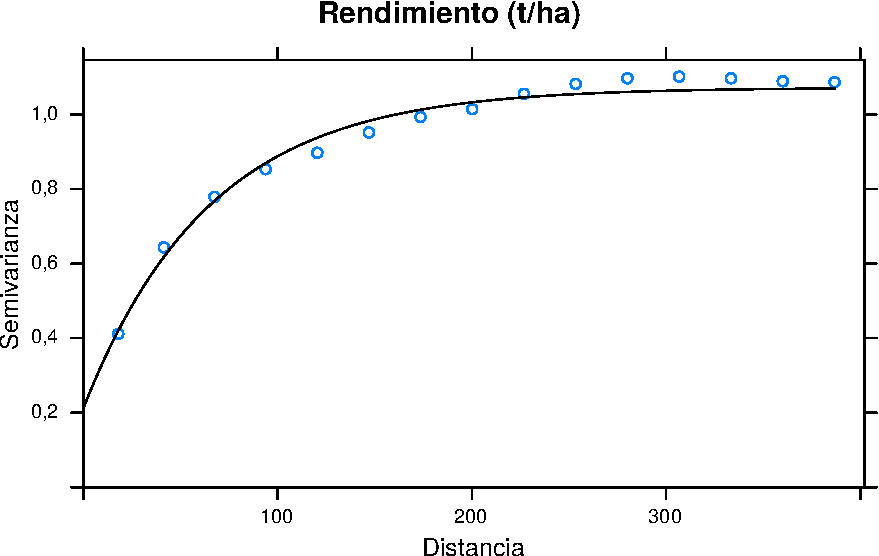
\includegraphics[width=\linewidth]{figuras/figLibro/unnamed-chunk-56-1} \end{center}

Las siguientes líneas permiten la visualización conjunta de los dos ajustes realizados.

\begin{Shaded}
\begin{Highlighting}[]
\NormalTok{vgLine <-}\StringTok{ }\KeywordTok{rbind}\NormalTok{(}
  \KeywordTok{cbind}\NormalTok{(}
    \KeywordTok{variogramLine}\NormalTok{(}
\NormalTok{      mod_exp, }\DataTypeTok{maxdist =} \KeywordTok{max}\NormalTok{(semiv_emp}\OperatorTok{$}\NormalTok{dist)),}
    \DataTypeTok{id =} \StringTok{"Exponencial"}\NormalTok{),}
  \KeywordTok{cbind}\NormalTok{(}
    \KeywordTok{variogramLine}\NormalTok{(}
\NormalTok{      mod_esf, }\DataTypeTok{maxdist =} \KeywordTok{max}\NormalTok{(semiv_emp}\OperatorTok{$}\NormalTok{dist)),}
    \DataTypeTok{id =} \StringTok{"Esférico"}\NormalTok{)}
\NormalTok{  )}


\KeywordTok{ggplot}\NormalTok{(semiv_emp, }\KeywordTok{aes}\NormalTok{(}\DataTypeTok{x =}\NormalTok{ dist, }\DataTypeTok{y =}\NormalTok{ gamma, }
                      \DataTypeTok{color =}\NormalTok{ id)) }\OperatorTok{+}
\StringTok{  }\KeywordTok{geom_line}\NormalTok{(}\DataTypeTok{data =}\NormalTok{ vgLine) }\OperatorTok{+}
\StringTok{  }\KeywordTok{geom_point}\NormalTok{() }\OperatorTok{+}
\StringTok{  }\KeywordTok{labs}\NormalTok{(}
    \DataTypeTok{title =} \StringTok{"Semivariograma experimental}
\StringTok{    y teórico ajustado"}\NormalTok{) }\OperatorTok{+}
\StringTok{  }\KeywordTok{xlab}\NormalTok{(}\StringTok{"Distancia"}\NormalTok{) }\OperatorTok{+}
\StringTok{  }\KeywordTok{ylab}\NormalTok{(}\StringTok{"Semivarianza"}\NormalTok{) }\OperatorTok{+}
\StringTok{  }\KeywordTok{scale_color_discrete}\NormalTok{(}
    \DataTypeTok{name =} \StringTok{"Modelo"}\NormalTok{,}
    \DataTypeTok{labels =} \KeywordTok{c}\NormalTok{(}\StringTok{"Esférico"}\NormalTok{, }
               \StringTok{"Exponencial"}\NormalTok{, }
               \StringTok{"Experimental"}\NormalTok{))}
\end{Highlighting}
\end{Shaded}

\begin{center}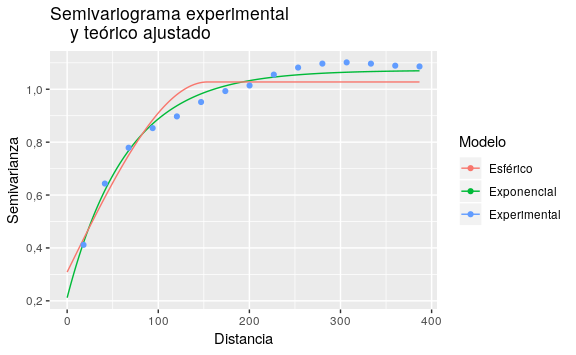
\includegraphics[width=\linewidth]{figuras/figLibro/unnamed-chunk-57-1} \end{center}

Algunas alternativas para aplicar las funciones de ajuste de los semivariogramas teóricos incluyen opciones de ajuste automático donde el usuario sólo especifica los modelos a ajustar sin tener que dar valores iniciales de los parámetros del semivariograma. La función estima valores iniciales razonables y selecciona aquel modelo de mejor bondad de ajuste en función a la SCE. A continuación, se presenta este ejemplo ajustando los modelos exponencial y esférico. Como era de esperar, el modelo de mejor ajuste fue el esférico.

\begin{Shaded}
\begin{Highlighting}[]
\NormalTok{modelos <-}\StringTok{ }\KeywordTok{fit.variogram}\NormalTok{(semiv_emp, }
                         \KeywordTok{vgm}\NormalTok{(}\KeywordTok{c}\NormalTok{(}\StringTok{"Exp"}\NormalTok{, }\StringTok{"Sph"}\NormalTok{)))}
\NormalTok{modelos}
\CommentTok{#>   model psill range}
\CommentTok{#> 1   Nug 0,212   0,0}
\CommentTok{#> 2   Exp 0,860  64,9}
\end{Highlighting}
\end{Shaded}

\begin{Shaded}
\begin{Highlighting}[]
\KeywordTok{attr}\NormalTok{(modelos, }\StringTok{'SSErr'}\NormalTok{)}
\CommentTok{#> [1] 0,377}
\end{Highlighting}
\end{Shaded}

Si bien, como se mostró en el análisis exploratorio de los datos no se evidencia una tendencia en la variable rendimiento con las coordenadas, en las siguientes líneas se ilustra cómo se realiza el ajuste del semivariograma empírico con tendencia dada por las coordenadas (x e y) y el posterior ajuste del modelo teórico. Los resultados muestran que no se observan diferencias importantes en los parámetros estimados del semivariograma teórico. En casos donde la tendencia es importante su efecto se puede reflejar en el ajuste del semivariograma empírico el cual suele mostrar un incremento de la semivarianza a medida que aumenta la distancia que no alcanza a estabilizarse dentro del dominio bajo estudio.

\begin{Shaded}
\begin{Highlighting}[]
\NormalTok{semiv_emp_t <-}\StringTok{ }\KeywordTok{variogram}\NormalTok{(Rinde }\OperatorTok{~}\StringTok{ }\NormalTok{x }\OperatorTok{+}\StringTok{ }\NormalTok{y, }
\NormalTok{                         datos_}\DecValTok{3}\NormalTok{, }\DataTypeTok{cutoff =} \DecValTok{400}\NormalTok{)}
\NormalTok{modelos_t <-}\StringTok{ }\KeywordTok{fit.variogram}\NormalTok{(semiv_emp_t, }
                           \KeywordTok{vgm}\NormalTok{(}\KeywordTok{c}\NormalTok{(}\StringTok{"Exp"}\NormalTok{, }\StringTok{"Sph"}\NormalTok{)))}
\NormalTok{modelos_t}
\CommentTok{#>   model psill range}
\CommentTok{#> 1   Nug 0,208   0,0}
\CommentTok{#> 2   Exp 0,859  63,8}
\KeywordTok{attr}\NormalTok{(modelos_t, }\StringTok{'SSErr'}\NormalTok{)}
\CommentTok{#> [1] 0,345}
\KeywordTok{plot}\NormalTok{(semiv_emp_t , modelos_t)}
\end{Highlighting}
\end{Shaded}

\begin{center}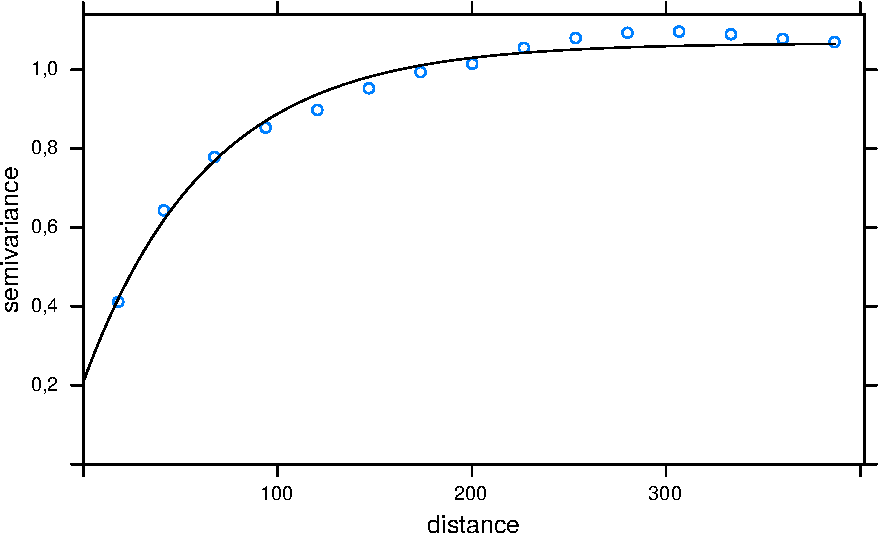
\includegraphics[width=\linewidth]{figuras/figLibro/unnamed-chunk-60-1} \end{center}

\hypertarget{mapeo-de-la-variabilidad-espacial}{%
\subsection{Mapeo de la variabilidad espacial}\label{mapeo-de-la-variabilidad-espacial}}

Para el mapeo de la variabilidad espacial se confeccionará una grilla de predicción donde se realiza el kriging. Las dimensiones de la grilla se establecerá mediante un polígono de los límites del lote. El archivo \textbf{limites.txt} contiene los puntos georreferenciados de cada arista del polígono.

\begin{Shaded}
\begin{Highlighting}[]
\NormalTok{limites <-}\StringTok{ }\KeywordTok{read.table}\NormalTok{(}\StringTok{"datos/limites.txt"}\NormalTok{, }
                      \DataTypeTok{header =} \OtherTok{TRUE}\NormalTok{)}
\KeywordTok{head}\NormalTok{(limites)}
\CommentTok{#>        x       y}
\CommentTok{#> 1 311842 5800614}
\CommentTok{#> 2 311950 5800728}
\CommentTok{#> 3 311998 5800788}
\CommentTok{#> 4 312006 5800835}
\CommentTok{#> 5 312566 5801431}
\CommentTok{#> 6 312590 5801435}
\end{Highlighting}
\end{Shaded}

La función \texttt{pred\_grid()} del paquete \texttt{geoR} genera una grilla regular de puntos de 10 metros de distancia entre estos. La función \texttt{polygrid()} recorta el polígono en la grilla siguiendo los límites del lote. Posteriormente se definen los nombres de las coordenadas y se transforma la clase del objeto a \texttt{sf} asignando el sistema de coordenadas.

\begin{Shaded}
\begin{Highlighting}[]
\NormalTok{grid <-}\StringTok{ }\KeywordTok{pred_grid}\NormalTok{(limites, }\DataTypeTok{by =} \DecValTok{10}\NormalTok{)}
\NormalTok{grid <-}\StringTok{ }\KeywordTok{polygrid}\NormalTok{(grid, }\DataTypeTok{bor =}\NormalTok{ limites)}

\KeywordTok{names}\NormalTok{(grid) <-}\StringTok{ }\KeywordTok{c}\NormalTok{(}\StringTok{"x"}\NormalTok{, }\StringTok{"y"}\NormalTok{)}
\NormalTok{grid <-}\StringTok{ }\KeywordTok{st_as_sf}\NormalTok{(grid, }\DataTypeTok{coords =} \KeywordTok{c}\NormalTok{(}\StringTok{"x"}\NormalTok{, }\StringTok{"y"}\NormalTok{),}
                 \DataTypeTok{crs =} \DecValTok{32721}\NormalTok{)}
\KeywordTok{plot}\NormalTok{(grid)}
\end{Highlighting}
\end{Shaded}

\begin{center}
\includegraphics[width=\linewidth]{figuras/figLibro/unnamed-chunk-62-1} \end{center}

La función \texttt{krige()} del paquete \texttt{gstat} realiza interpolación kriging y simulaciones condicionales mediante diferentes métodos de predicción. En este caso, se presenta la interpolación por kriging ordinario con el modelo de semivariograma exponencial estimado con geoestadística clásica. Los argumentos de esta función incluyen, la fórmula en la cual se especifica que el proceso es estacionario (\texttt{Rinde\textasciitilde{}1}), la base de datos (\texttt{datos\_3}), el objeto sobre el cual se hará la predicción (\texttt{grid}) y la información del modelo del modelo de semivariograma teórico ajustado (\texttt{model}) La información de este último se encuentra dentro del objeto \texttt{modelos}. Los argumentos \texttt{nmin} y \texttt{nmax} permiten realizar el proceso de interpolación en un contexto local, con un número mínimo y máximo de vecinos de cada punto a predecir de 7 y 25, respectivamente. En caso de omitir estos últimos argumentos la interpolación se realiza en un contexto global.

\begin{Shaded}
\begin{Highlighting}[]
\NormalTok{kriging_o <-}
\StringTok{  }\KeywordTok{krige}\NormalTok{(}
\NormalTok{    Rinde }\OperatorTok{~}\StringTok{ }\DecValTok{1}\NormalTok{,}
\NormalTok{    datos_}\DecValTok{3}\NormalTok{,}
    \KeywordTok{st_as_sf}\NormalTok{(grid),}
    \DataTypeTok{nmin =} \DecValTok{7}\NormalTok{,}
    \DataTypeTok{nmax =} \DecValTok{25}\NormalTok{,}
    \DataTypeTok{model =}\NormalTok{ modelos}
\NormalTok{  ) }
\CommentTok{#> [using ordinary kriging]}
\end{Highlighting}
\end{Shaded}

A continuación, se realiza la visualización de la predicción y su varianza.

\begin{Shaded}
\begin{Highlighting}[]
\NormalTok{predK_otm <-}\StringTok{ }\KeywordTok{tm_shape}\NormalTok{(kriging_o) }\OperatorTok{+}
\StringTok{  }\KeywordTok{tm_dots}\NormalTok{(}\StringTok{"var1.pred"}\NormalTok{, }\DataTypeTok{style =} \StringTok{"cont"}\NormalTok{,}
          \DataTypeTok{title =} \StringTok{"Predicción")}
\StringTok{varK_otm <-  tm_shape(kriging_o) +}
\StringTok{  tm_dots("}\NormalTok{var1.var}\StringTok{", style = "}\NormalTok{cont}\StringTok{",}
\StringTok{          title = "}\NormalTok{Varianza}\StringTok{")}

\StringTok{tmap_arrange(predK_otm, varK_otm)}
\end{Highlighting}
\end{Shaded}

\begin{center}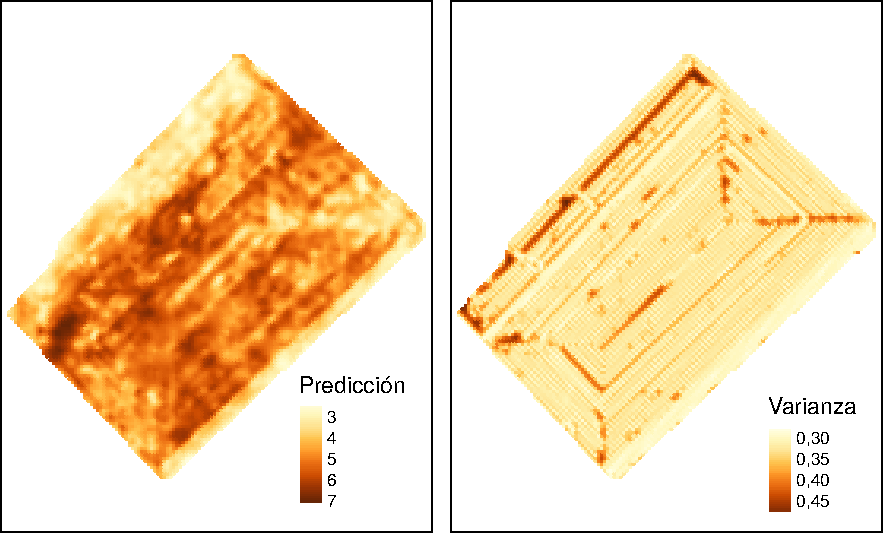
\includegraphics[width=\linewidth]{figuras/figLibro/unnamed-chunk-64-1} \end{center}

La siguiente línea de comando permite realizar la predicción kriging en bloques en un contexto local para lo cual solo se adiciona en la función \texttt{krige()} el argumento \texttt{block}. En este ejemplo se definió la dimensión del bloque de \(40 \times 40\) m. Posteriormente se realiza la visualización de forma similar al caso anterior.

\begin{Shaded}
\begin{Highlighting}[]
\NormalTok{kriging_b <-}
\StringTok{  }\KeywordTok{krige}\NormalTok{(}
\NormalTok{    Rinde }\OperatorTok{~}\StringTok{ }\DecValTok{1}\NormalTok{,}
\NormalTok{    datos_}\DecValTok{3}\NormalTok{,}
\NormalTok{    grid ,}
    \DataTypeTok{nmin =} \DecValTok{7}\NormalTok{,}
    \DataTypeTok{nmax =} \DecValTok{25}\NormalTok{,}
    \DataTypeTok{model =}\NormalTok{ modelos,}
    \DataTypeTok{block =} \KeywordTok{c}\NormalTok{(}\DecValTok{40}\NormalTok{, }\DecValTok{40}\NormalTok{)}
\NormalTok{  )}
\CommentTok{#> [using ordinary kriging]}
\end{Highlighting}
\end{Shaded}

\begin{Shaded}
\begin{Highlighting}[]

\NormalTok{predK_btm <-}\StringTok{ }\KeywordTok{tm_shape}\NormalTok{(kriging_b) }\OperatorTok{+}
\StringTok{  }\KeywordTok{tm_dots}\NormalTok{(}\StringTok{"var1.pred"}\NormalTok{, }\DataTypeTok{style =} \StringTok{"cont"}\NormalTok{,}
          \DataTypeTok{title =} \StringTok{"Predicción Bloque"}\NormalTok{)}
\NormalTok{varK_btm <-}\StringTok{  }\KeywordTok{tm_shape}\NormalTok{(kriging_b) }\OperatorTok{+}
\StringTok{  }\KeywordTok{tm_dots}\NormalTok{(}\StringTok{"var1.var"}\NormalTok{, }\DataTypeTok{style =} \StringTok{"cont"}\NormalTok{,}
          \DataTypeTok{title =} \StringTok{"Varianza Bloque"}\NormalTok{)}

\KeywordTok{tmap_arrange}\NormalTok{(predK_btm, varK_btm)}
\end{Highlighting}
\end{Shaded}

\begin{center}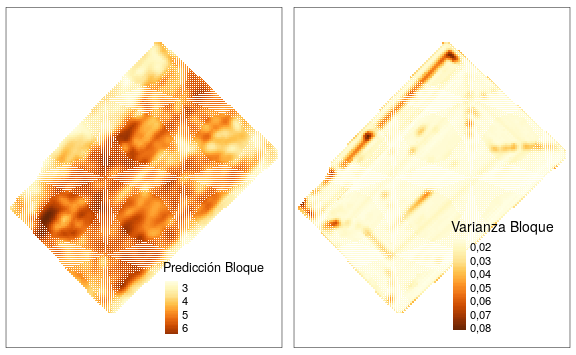
\includegraphics[width=\linewidth]{figuras/figLibro/unnamed-chunk-66-1} \end{center}

Las siguientes líneas de código muestran cómo obtener un \texttt{data.frame} conteniendo las predicciones realizadas sobre la grilla. En primer lugar, se extraen las coordenadas del objeto \texttt{kriging\_b} y luego se transforma la clase del objeto a \texttt{data.frame}.

\begin{Shaded}
\begin{Highlighting}[]
\NormalTok{kriging_b}\OperatorTok{$}\NormalTok{x <-}\StringTok{ }\KeywordTok{st_coordinates}\NormalTok{(kriging_b)[, }\DecValTok{1}\NormalTok{]}
\NormalTok{kriging_b}\OperatorTok{$}\NormalTok{y <-}\StringTok{ }\KeywordTok{st_coordinates}\NormalTok{(kriging_b)[, }\DecValTok{2}\NormalTok{]}
\NormalTok{predRinde <-}\StringTok{ }
\StringTok{  }\KeywordTok{data.frame}\NormalTok{(kriging_b)[, }\KeywordTok{c}\NormalTok{(}\StringTok{"x"}\NormalTok{, }\StringTok{"y"}\NormalTok{, }
                            \StringTok{"var1.pred"}\NormalTok{)]}
\KeywordTok{names}\NormalTok{(predRinde)[}\DecValTok{3}\NormalTok{] <-}\StringTok{ }\KeywordTok{paste}\NormalTok{(}\StringTok{"Tg"}\NormalTok{)}
\end{Highlighting}
\end{Shaded}

En el caso que exista una tendencia dada por las coordenadas, se utiliza kriging universal como método de interpolación espacial. Los comandos son similares a los anteriores, sólo debe cambiarse la fórmula. Por ejemplo, para una tendencia de primer grado en las coordenadas espaciales se escribiría \texttt{Rinde\textasciitilde{}x+y}. El modelo de semivariograma que se utiliza debe haberse ajustando contemplado el mismo tipo de tendencia. En situaciones donde otras covariables explican la tendencia en la media, éstas deben especificarse en la fórmula. Para poder hacer la interpolación es necesario que los valores de las covariables también estén disponibles en la grilla de predicción. En este último caso la interpolación se denomina kriging con deriva externa.

La interpolación también puede hacerse utilizando los parámetros \emph{partial sill}, rango y \emph{nugget} del semivariograma estimado con REML. Para el ajuste de un MLM con errores correlacionados espacialmente vía REML, la base de datos no debe ser muy grande. Para poder realizar el ajuste de un MLM en el conjunto de datos de ilustración, se tomó una muestra aleatoria de n=500 sobre la base de datos original de n=9009, usando la función \texttt{sample()}. Las siguientes líneas de código muestran el ajuste del semivariograma y obtención de los parámetros del mismo usando la función \texttt{gls()} del paquete \texttt{nlme}. Se realiza el ajuste de dos modelos lineales, el primero sin correlación espacial (\texttt{null\_model}) y el segundo con una estructura de correlación espacial del tipo exponencial (\texttt{esp\_model}).

\begin{Shaded}
\begin{Highlighting}[]
\KeywordTok{set.seed}\NormalTok{(}\DecValTok{7}\NormalTok{)}
\NormalTok{datos_}\DecValTok{4}\NormalTok{ <-}\StringTok{ }\NormalTok{datos_}\DecValTok{3}\NormalTok{[}
  \KeywordTok{sample}\NormalTok{(}\DecValTok{1}\OperatorTok{:}\KeywordTok{nrow}\NormalTok{(datos_}\DecValTok{3}\NormalTok{), }
         \DecValTok{500}\NormalTok{, }\DataTypeTok{replace =} \OtherTok{FALSE}\NormalTok{), ]}
\NormalTok{null_model <-}
\StringTok{  }\KeywordTok{gls}\NormalTok{(Rinde }\OperatorTok{~}\StringTok{ }\DecValTok{1}\NormalTok{, datos_}\DecValTok{4}\NormalTok{, }
      \DataTypeTok{method =} \StringTok{"REML"}\NormalTok{, }
      \DataTypeTok{na.action =}\NormalTok{ na.omit)}

\NormalTok{esp_model <-}\StringTok{ }\KeywordTok{gls}\NormalTok{(}
\NormalTok{  Rinde }\OperatorTok{~}\StringTok{ }\DecValTok{1}\NormalTok{,}
  \DataTypeTok{data =}\NormalTok{ datos_}\DecValTok{4}\NormalTok{,}
  \DataTypeTok{correlation =} \KeywordTok{corExp}\NormalTok{(}
    \DataTypeTok{form =}  \OperatorTok{~}\StringTok{ }\NormalTok{x }\OperatorTok{+}\StringTok{ }\NormalTok{y,}
    \DataTypeTok{metric =} \StringTok{"euclidean"}\NormalTok{,}
    \DataTypeTok{nugget =}\NormalTok{ T}
\NormalTok{  ),}
  \DataTypeTok{method =} \StringTok{"REML"}\NormalTok{,}
  \DataTypeTok{na.action =}\NormalTok{ na.omit}
\NormalTok{)}
\end{Highlighting}
\end{Shaded}

A continuación, se realiza la comparación de ambos modelos mediante la prueba del cociente de verosimilitud. Los resultados muestran que hay diferencias significativas (p\textless{}0.005) entre ambos modelos, con lo cual se elige el modelo espacial. Los valores de AIC y BIC también mostraban un mejor ajuste de este último.

\begin{Shaded}
\begin{Highlighting}[]
\KeywordTok{anova}\NormalTok{(null_model, esp_model)}
\CommentTok{#> Model df AIC BIC logLik Test L.Ratio p-value}
\CommentTok{#> null_model 1 2 1526 1535 -761}
\CommentTok{#> esp_model 2 4 1230 1247 -611 1 vs 2 300}
\OperatorTok{<}\NormalTok{.}\DecValTok{0001}
\end{Highlighting}
\end{Shaded}

Con el modelo ajustado se obtienen los parámetros del semivariograma y se construye el objeto \texttt{m} que contendrá estos para su posterior interpolación vía kriging.

\begin{Shaded}
\begin{Highlighting}[]
\KeywordTok{summary}\NormalTok{(esp_model)}
\CommentTok{#> Generalized least squares fit by REML}
\CommentTok{#> Model: Rinde ~ 1}
\CommentTok{#> Data: datos_4}
\CommentTok{#> AIC BIC logLik}
\CommentTok{#> 1230 1247 -611}
\CommentTok{#>}
\CommentTok{#> Correlation Structure: Exponential spatial}
\NormalTok{correlation}
\CommentTok{#> Formula: ~x + y}
\CommentTok{#> Parameter estimate(s):}
\CommentTok{#> range nugget}
\CommentTok{#> 102,547 0,134}
\CommentTok{#>}
\CommentTok{#> Coefficients:}
\CommentTok{#> Value Std.Error t-value p-value}
\CommentTok{#> (Intercept) 4,22 0,234 18 0}
\CommentTok{#>}
\CommentTok{#> Standardized residuals:}
\CommentTok{#> Min Q1 Med Q3 Max}
\CommentTok{#> -1,848 -0,371 0,378 1,097 2,634}
\CommentTok{#>}
\CommentTok{#> Residual standard error: 1,18}
\CommentTok{#> Degrees of freedom: 500 total; 499 residual}
\NormalTok{esp_model}\OperatorTok{$}\NormalTok{sigma}
\CommentTok{#> [1] 1,18}
\NormalTok{nugget <-}\StringTok{ }\FloatTok{0.1344285} \OperatorTok{*}\StringTok{ }\NormalTok{esp_model}\OperatorTok{$}\NormalTok{sigma }\OperatorTok{^}\StringTok{ }\DecValTok{2}
\NormalTok{psill <-}\StringTok{ }\NormalTok{esp_model}\OperatorTok{$}\NormalTok{sigma }\OperatorTok{^}\StringTok{ }\DecValTok{2} \OperatorTok{-}\StringTok{ }\NormalTok{nugget}
\NormalTok{range <-}\StringTok{ }\FloatTok{102.5470883}

\NormalTok{m <-}\StringTok{ }\KeywordTok{vgm}\NormalTok{(psill, }\StringTok{"Exp"}\NormalTok{, range, nugget)}
\NormalTok{kriging_mlm <-}
\StringTok{  }\KeywordTok{krige}\NormalTok{(}
\NormalTok{    Rinde }\OperatorTok{~}\StringTok{ }\DecValTok{1}\NormalTok{,}
\NormalTok{    datos_}\DecValTok{4}\NormalTok{,}
\NormalTok{    grid ,}
    \DataTypeTok{nmin =} \DecValTok{7}\NormalTok{,}
    \DataTypeTok{nmax =} \DecValTok{25}\NormalTok{,}
    \DataTypeTok{model =}\NormalTok{ m}
\NormalTok{  )}
\CommentTok{#> [using ordinary kriging]}
\end{Highlighting}
\end{Shaded}

El mismo ajuste de semivariograma puede realizarse utilizando la función \texttt{likfit()} del paquete \texttt{geoR}. En este caso es necesario generar un objeto del tipo \texttt{geodata}. La función de ajuste solicita valores iniciales de \emph{sill} parcial y rango y modelo teórico (para esta aplicación se usa el exponencial). En el caso del efecto \emph{nugget} el mismo es estimado por defecto. Es posible también incorporar tendencias utilizando el argumento \texttt{trend}. Los resultados del modelo muestran valores estimados de los parámetros similares a los obtenidos con la función \texttt{gls()}.

\begin{Shaded}
\begin{Highlighting}[]
\NormalTok{datos_geor <-}\StringTok{ }\KeywordTok{as.data.frame}\NormalTok{(datos_}\DecValTok{4}\NormalTok{)}
\NormalTok{datos_geor <-}
\StringTok{  }\KeywordTok{as.geodata}\NormalTok{(datos_geor,}
             \DataTypeTok{coords.col =} \KeywordTok{c}\NormalTok{(}\StringTok{"x"}\NormalTok{, }\StringTok{"y"}\NormalTok{),}
             \DataTypeTok{data.col =} \StringTok{"Rinde"}\NormalTok{)}

\NormalTok{mlm_geor <-}
\StringTok{  }\KeywordTok{likfit}\NormalTok{(}
\NormalTok{    datos_geor,}
    \DataTypeTok{ini =} \KeywordTok{c}\NormalTok{(}\FloatTok{0.7}\NormalTok{, }\DecValTok{90}\NormalTok{),}
    \DataTypeTok{cov.model =} \StringTok{"exponential"}\NormalTok{,}
    \DataTypeTok{lik.method =} \StringTok{"REML"}\NormalTok{,}
    \DataTypeTok{messages =} \OtherTok{FALSE}
\NormalTok{  )}
\KeywordTok{summary}\NormalTok{(mlm_geor)}
\CommentTok{#> Summary of the parameter estimation}
\CommentTok{#> -----------------------------------}
\CommentTok{#> Estimation method: restricted maximum}
\NormalTok{likelihood}
\CommentTok{#>}
\CommentTok{#> Parameters of the mean component (trend):}
\CommentTok{#> beta}
\CommentTok{#> 4,22}
\CommentTok{#>}
\CommentTok{#> Parameters of the spatial component:}
\CommentTok{#> correlation function: exponential}
\CommentTok{#> (estimated) variance parameter sigmasq}
\NormalTok{(partial sill) =}\StringTok{ }\DecValTok{1}\NormalTok{,}\DecValTok{2}
\CommentTok{#> (estimated) cor. fct. parameter phi (range}
\NormalTok{parameter}\ErrorTok{)}\NormalTok{ =}\StringTok{ }\DecValTok{103}
\CommentTok{#> anisotropy parameters:}
\CommentTok{#> (fixed) anisotropy angle = 0 ( 0 degrees )}
\CommentTok{#> (fixed) anisotropy ratio = 1}
\CommentTok{#>}
\CommentTok{#> Parameter of the error component:}
\CommentTok{#> (estimated) nugget = 0,186}
\CommentTok{#>}
\CommentTok{#> Transformation parameter:}
\CommentTok{#> (fixed) Box-Cox parameter = 1 (no}
\NormalTok{transformation}\ErrorTok{)}
\CommentTok{#>}
\CommentTok{#> Practical Range with cor=0.05 for asymptotic}
\NormalTok{range}\OperatorTok{:}\StringTok{ }\DecValTok{307}
\CommentTok{#>}
\CommentTok{#> Maximised Likelihood:}
\CommentTok{#> log.L n.params AIC BIC}
\CommentTok{#> "-608" "4" "1224" "1241"}
\CommentTok{#>}
\CommentTok{#> non spatial model:}
\CommentTok{#> log.L n.params AIC BIC}
\CommentTok{#> "-758" "2" "1520" "1528"}
\CommentTok{#>}
\CommentTok{#> Call:}
\CommentTok{#> likfit(geodata = datos_geor, ini.cov.pars =}
\KeywordTok{c}\NormalTok{(}\FloatTok{0.7}\NormalTok{, }\DecValTok{90}\NormalTok{), cov.model =}\StringTok{ "exponential"}\NormalTok{,}
\CommentTok{#> lik.method = "REML", messages = FALSE)}
\end{Highlighting}
\end{Shaded}

\hypertarget{validaciuxf3n-cruzada-1}{%
\subsection{Validación cruzada}\label{validaciuxf3n-cruzada-1}}

A continuación, se ilustra el proceso de validación cruzada \emph{k-fold}. En este caso la función utilizada es \texttt{krige.cv()} del paquete \texttt{gstat}. Aquí como en el ajuste del semivariogram empírico y la interpolación, se tienen los argumentos fórmula (\texttt{Rinde\textasciitilde{}1}, lo cual especifica que es un proceso estacionario), la base de datos (\texttt{datos\_3}) y el modelo de semivariograma teórico ajustado (\texttt{modelos}). Aquí también se realiza la validación usando kriging en un contexto local por lo que se colocan los argumentos \texttt{nmin} y \texttt{nmax}. El argumento \texttt{nfold} determina el número de grupos (k) en los que se divide la base de datos para realizar la validación cruzada \emph{k-fold}. Para obtener repetibilidad en los resultados se sugiere fijar la semilla mediante la función \texttt{set.seed()}.

\begin{Shaded}
\begin{Highlighting}[]
\KeywordTok{set.seed}\NormalTok{(}\DecValTok{17}\NormalTok{)}
\NormalTok{valcru <-}
\StringTok{  }\KeywordTok{krige.cv}\NormalTok{(}
\NormalTok{    Rinde }\OperatorTok{~}\StringTok{ }\DecValTok{1}\NormalTok{,}
\NormalTok{    datos_}\DecValTok{3}\NormalTok{,}
\NormalTok{    modelos,}
    \DataTypeTok{nfold =} \DecValTok{10}\NormalTok{,}
    \DataTypeTok{nmin =} \DecValTok{7}\NormalTok{,}
    \DataTypeTok{nmax =} \DecValTok{25}
\NormalTok{  )}
\end{Highlighting}
\end{Shaded}

Realizada la validación es posible calcular estadísticos resumen como el error medio (ME), error cuadrático medio (MSE), media del cociente de la desviación cuadrática (\emph{mean squared deviation ratio}, MSDR), raíz del error cuadrático medio (RMSE), la RMSE relativa a la media de los observados (RMSE\_rel) y la correlación lineal entre los observados vs.~Predichos. Un gráfico de estos últimos se muestra al final.

\begin{Shaded}
\begin{Highlighting}[]
\NormalTok{ME <-}\StringTok{ }\KeywordTok{mean}\NormalTok{(valcru}\OperatorTok{$}\NormalTok{residual)}
\NormalTok{MSE <-}\StringTok{ }\KeywordTok{mean}\NormalTok{(valcru}\OperatorTok{$}\NormalTok{residual }\OperatorTok{^}\StringTok{ }\DecValTok{2}\NormalTok{)}
\NormalTok{MSDR <-}\StringTok{ }\KeywordTok{mean}\NormalTok{(valcru}\OperatorTok{$}\NormalTok{zscore }\OperatorTok{^}\StringTok{ }\DecValTok{2}\NormalTok{)}
\NormalTok{RMSE <-}\StringTok{ }\KeywordTok{sqrt}\NormalTok{(}\KeywordTok{mean}\NormalTok{(valcru}\OperatorTok{$}\NormalTok{residual }\OperatorTok{^}\StringTok{ }\DecValTok{2}\NormalTok{))}
\NormalTok{RMSE_rel <-}\StringTok{ }
\StringTok{  }\KeywordTok{sqrt}\NormalTok{(}\KeywordTok{mean}\NormalTok{(valcru}\OperatorTok{$}\NormalTok{residual }\OperatorTok{^}\StringTok{ }\DecValTok{2}\NormalTok{)) }\OperatorTok{/}\StringTok{ }
\StringTok{  }\KeywordTok{mean}\NormalTok{(valcru}\OperatorTok{$}\NormalTok{observed) }\OperatorTok{*}\StringTok{ }\DecValTok{100}
\NormalTok{r <-}\StringTok{ }\KeywordTok{cor}\NormalTok{(valcru}\OperatorTok{$}\NormalTok{observed, }
\NormalTok{         valcru}\OperatorTok{$}\NormalTok{observed }\OperatorTok{-}\StringTok{ }\NormalTok{valcru}\OperatorTok{$}\NormalTok{residual)}

\NormalTok{tabla <-}\StringTok{ }\KeywordTok{data.frame}\NormalTok{(ME, MSE, RMSE, }
\NormalTok{                    RMSE_rel, MSDR, r)}
\NormalTok{tabla}
\CommentTok{#>         ME   MSE  RMSE RMSE_rel  MSDR     r}
\CommentTok{#> 1 -0,00018 0,228 0,478     10,3 0,665 0,899}
\KeywordTok{plot}\NormalTok{(}
\NormalTok{  valcru}\OperatorTok{$}\NormalTok{observed,}
\NormalTok{  valcru}\OperatorTok{$}\NormalTok{observed }\OperatorTok{-}\StringTok{ }\NormalTok{valcru}\OperatorTok{$}\NormalTok{residual,}
  \DataTypeTok{xlab =} \StringTok{"Observados"}\NormalTok{,}
  \DataTypeTok{ylab =} \StringTok{"Predichos"}
\NormalTok{)}
\end{Highlighting}
\end{Shaded}

\begin{center}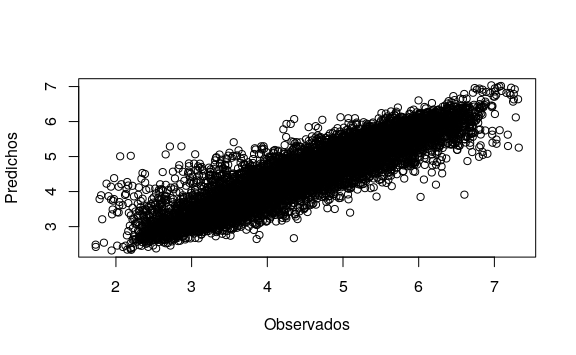
\includegraphics[width=\linewidth]{figuras/figLibro/unnamed-chunk-73-1} \end{center}

\hypertarget{caracterizaciuxf3n-de-variabilidad-espacial-con-muxfaltiples-capas-de-datos-1}{%
\section{Caracterización de variabilidad espacial con múltiples capas de datos}\label{caracterizaciuxf3n-de-variabilidad-espacial-con-muxfaltiples-capas-de-datos-1}}

\hypertarget{anuxe1lisis-de-componentes-principales-1}{%
\subsection{Análisis de componentes principales}\label{anuxe1lisis-de-componentes-principales-1}}

Para implementar el análisis multivariado es necesario contar con información de cada variable en los mismos sitios georreferenciados. En esta sección se usa la base de datos \textbf{Pred2.txt} que contiene mediciones de conductividad eléctrica aparente en dos profundidades 0-30 cm (CE30) y 0-90 cm (CE90), elevación (Elev), profundidad de suelo (Pe) y rendimiento de trigo (Tg). Para generar esta base debido a las diferentes resoluciones espaciales de las variables medidas, se calculó una zona buffer de 15 m de radio para la variable Pe y sobre cada punto buffer se calculó la mediana de las restantes variables. La matriz de datos resultante quedó conformada por n=482 sitios (filas) y p=7 variables (columnas).

Para realizar el Análisis de Componentes Principales espacial (MULTISPATI-PCA) se utiliza los paquetes \texttt{ade4} y \texttt{adespatial}. Primero se necesita calcular la matriz de ponderación espacial en forma similar a la realizada para el cálculo del índice de Moran. Luego, se realiza un Análisis de Componentes Principales (PCA) clásico y posteriormente sobre las componentes generadas por PCA, se aplica el MULTISPATI-PCA.

Carga de base de datos multivariada.

\begin{Shaded}
\begin{Highlighting}[]
\NormalTok{pred <-}\StringTok{ }\KeywordTok{read.table}\NormalTok{(}\StringTok{"datos/Pred2.txt"}\NormalTok{, }
                   \DataTypeTok{header =} \OtherTok{TRUE}\NormalTok{)}
\KeywordTok{head}\NormalTok{(pred)}
\CommentTok{#> x y Pe Elev CE30 CE90 Tg}
\CommentTok{#> 1 312283 5800205 80 161 21,8 30,6 4,19}
\CommentTok{#> 2 312257 5800229 40 161 30,3 17,9 4,00}
\CommentTok{#> [ reached 'max'}
    \OperatorTok{/}\StringTok{ }\KeywordTok{getOption}\NormalTok{(}\StringTok{"max.print"}\NormalTok{) }\OperatorTok{--}
\NormalTok{omitted }\DecValTok{4}\NormalTok{ rows ]}
\end{Highlighting}
\end{Shaded}

La función \texttt{dudi.pca()} del paquete \texttt{ade4}, permite realizar un PCA sobre objetos de clase \texttt{data.frame}. Sus argumentos indican, las variables con las que se realizará el PCA, un valor lógico (\texttt{TRUE} o \texttt{FALSE}) indicando si debe o no centrarse por la media (\texttt{center}) y normalizarse (\texttt{scale}), un valor lógico para la realización o no del gráfico (\texttt{scannf}) y la cantidad de ejes guardados (\texttt{nf}), que coincide con la cantidad de variables utilizadas en el análisis.

\begin{Shaded}
\begin{Highlighting}[]
\NormalTok{pca <-}
\StringTok{  }\KeywordTok{dudi.pca}\NormalTok{(}
\NormalTok{    pred[, }\DecValTok{3}\OperatorTok{:}\DecValTok{7}\NormalTok{],}
    \DataTypeTok{center =} \OtherTok{TRUE}\NormalTok{,}
    \DataTypeTok{scale =} \OtherTok{TRUE}\NormalTok{,}
    \DataTypeTok{scannf =} \OtherTok{FALSE}\NormalTok{,}
    \DataTypeTok{nf =} \DecValTok{5}
\NormalTok{  )}
\end{Highlighting}
\end{Shaded}

Para transformar un PCA en un PCA espacial (MULTISPATI-PCA) se calcula la red de vecindarios y la matriz de ponderación espacial. La distancia máxima para definir los sitios vecinos de cada dato fue de 45 m. Además, se adiciona el argumento \texttt{zero.policy=T} para poder generar la matriz de pesos espaciales contemplando que algunos puntos no tengan datos vecinos. La función \texttt{multispati()} permite realizar el MUlTISPATI-PCA. Para ello es necesario colocar en la función el objeto que surge de realizar el ACP (pca) y la matriz de pesos espaciales (\texttt{pesos\_sp}). El argumento \texttt{nfposi} hace referencia al número de ejes con autocorrelación positiva que es retenido en el análisis. También pueden guardarse ejes con autocorrelación negativa mediante el argumento \texttt{nfnega}. En general los ejes con autocorrelación negativa son aquellos de menor contribución a la variabilidad total.

\begin{Shaded}
\begin{Highlighting}[]
\NormalTok{cord <-}\StringTok{ }\KeywordTok{coordinates}\NormalTok{(pred[, }\DecValTok{1}\OperatorTok{:}\DecValTok{2}\NormalTok{])}
\NormalTok{vecindarios <-}\StringTok{ }\KeywordTok{dnearneigh}\NormalTok{(cord, }\DecValTok{0}\NormalTok{, }\DecValTok{45}\NormalTok{)}
\NormalTok{pesos_sp <-}\StringTok{ }\KeywordTok{nb2listw}\NormalTok{(vecindarios, }
                     \DataTypeTok{style =} \StringTok{"W"}\NormalTok{, }
                     \DataTypeTok{zero.policy =}\NormalTok{ T)}

\NormalTok{pca_esp <-}
\StringTok{  }\NormalTok{adespatial}\OperatorTok{::}\KeywordTok{multispati}\NormalTok{(pca, pesos_sp, }
                         \DataTypeTok{scannf =}\NormalTok{ F, }\DataTypeTok{nfposi =} \DecValTok{5}\NormalTok{)}
\end{Highlighting}
\end{Shaded}

Para realizar un gráfico que muestre las correlaciones entre las variables se puede usar la función \texttt{s.arrow()}. En este gráfico de traza un vector para cada variable en el espacio definido por las componentes principales que se seleccionen. En este caso de estudio, la función utiliza la primera componente para graficar el eje horizontal y la segunda componente para el eje vertical. Para adicionar un gráfico de barras con los autovalores puede usarse el argumento \texttt{add.scatter.eig()}.

\begin{Shaded}
\begin{Highlighting}[]
\KeywordTok{s.arrow}\NormalTok{(pca_esp}\OperatorTok{$}\NormalTok{c1,}
        \DataTypeTok{xax =} \DecValTok{1}\NormalTok{,}
        \DataTypeTok{yax =} \DecValTok{2}\NormalTok{,}
        \DataTypeTok{clabel =} \DecValTok{1}\NormalTok{)}
\KeywordTok{add.scatter.eig}\NormalTok{(}
\NormalTok{  pca_esp}\OperatorTok{$}\NormalTok{eig,}
  \DataTypeTok{xax =} \DecValTok{1}\NormalTok{,}
  \DataTypeTok{yax =} \DecValTok{2}\NormalTok{,}
  \DataTypeTok{posi =} \StringTok{"bottomright"}\NormalTok{,}
  \DataTypeTok{ratio =} \FloatTok{0.2}
\NormalTok{)}
\end{Highlighting}
\end{Shaded}

\begin{center}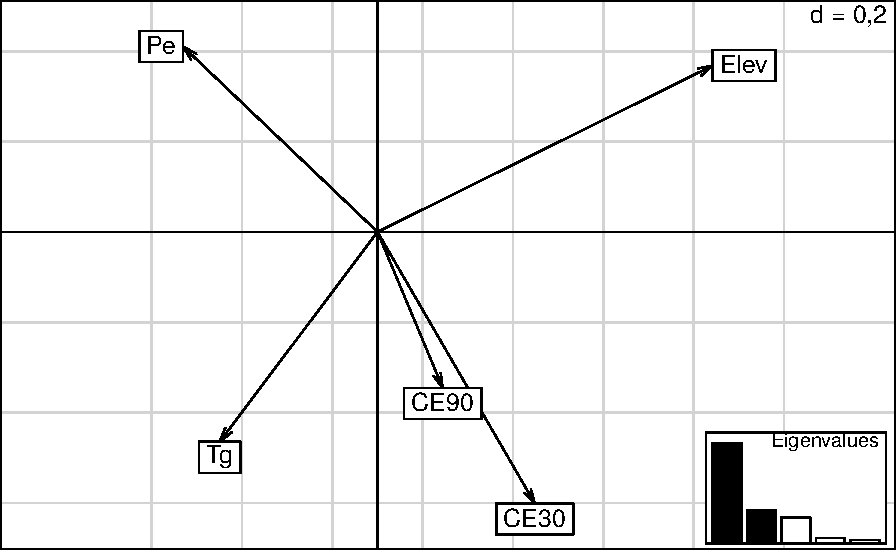
\includegraphics[width=\linewidth]{figuras/figLibro/unnamed-chunk-77-1} \end{center}

El gráfico obtenido del MULTISPATI-PCA muestra que las variables Elev y Pe son las más importantes en la explicación de la variabilidad espacial a nivel del primer eje (sPC1, eje horizontal). Mientras que la CE30 y Tg presentan mayor importancia en la SPC2. Además, se observa una correlación positiva entre CE30 y CE90, y negativa entre estas dos y la Pe. También la Elev y Tg se correlacionan en forma negativa. El gráfico de autovalores (barras) sugiere dos estructuras principales a nivel de sPC1 y sPC2, siempre la sPC1 explica la mayor parte de la variabilidad de los datos seguida por sPC2, sPC3, y así sucesivamente.

\begin{Shaded}
\begin{Highlighting}[]
\KeywordTok{summary}\NormalTok{(pca_esp)}
\CommentTok{#>}
\CommentTok{#> Multivariate Spatial Analysis}
\CommentTok{#> Call: adespatial::multispati(dudi = pca,}
\NormalTok{listw =}\StringTok{ }\NormalTok{pesos_sp, scannf =}\StringTok{ }\NormalTok{F,}
\CommentTok{#> nfposi = 5)}
\CommentTok{#>}
\CommentTok{#> Scores from the initial duality diagram:}
\CommentTok{#> var cum ratio moran}
\CommentTok{#> RS1 1,936 1,94 0,387 0,676}
\CommentTok{#> RS2 1,078 3,01 0,603 0,405}
\CommentTok{#> RS3 0,878 3,89 0,778 0,250}
\CommentTok{#> RS4 0,628 4,52 0,904 0,552}
\CommentTok{#> [ reached 'max'}
    \OperatorTok{/}\StringTok{ }\KeywordTok{getOption}\NormalTok{(}\StringTok{"max.print"}\NormalTok{) }\OperatorTok{--}
\NormalTok{omitted }\DecValTok{1}\NormalTok{ rows ]}
\CommentTok{#>}
\CommentTok{#> Multispati eigenvalues decomposition:}
\CommentTok{#> eig var moran}
\CommentTok{#> CS1 1,4254 1,808 0,7884}
\CommentTok{#> CS2 0,4684 1,095 0,4277}
\CommentTok{#> CS3 0,3712 0,748 0,4963}
\CommentTok{#> CS4 0,0790 0,689 0,1147}
\CommentTok{#> CS5 0,0484 0,660 0,0734}
\end{Highlighting}
\end{Shaded}

Como se establece en la literatura, MULTISPATI-PCA maximiza el producto entre la varianza espacial y la autocorrelación mientras que PCA maximiza la varianza total. Los resultados muestran que con MULTISPATIPCA se explica una menor proporción de la varianza acumulada en el primer eje, respecto de PCA (1,81 vs.~1,94). Las dos primeras CP del PCA explican 60\% de la variabilidad total mientras que la CS1 y CS2 del MULTISPATI el 58\%. No obstante, los valores del índice de Moran calculados para las tres primeras CPs sugieren que la estimación de autocorrelación aumentó cuando se usó MULTISPATIPCA respecto de la contenida en las CPs del PCA (0,79 vs.~0,68 para el eje 1, 0,43 vs.~0,40 para el eje 2, 0,50 vs.~0,25 para el eje 3). Este resultado permitiría una visualización mejor de la variabilidad espacial. Por el contrario, a nivel de las CPs 4 y 5 este comportamiento fue inverso.

\hypertarget{anuxe1lisis-de-conglomerados-1}{%
\subsection{Análisis de conglomerados}\label{anuxe1lisis-de-conglomerados-1}}

Para implementar este análisis también es necesario contar con información de cada variable en los mismos sitios georreferenciados. Otra forma de lograr esto es interpolar cada una de ellas con la misma grilla de predicción. Es decir, que cada punto de la grilla tendrá un dato para cada variable predicha. Para el siguiente caso de estudio se realizó el procedimiento de interpolación con mediciones de conductividad eléctrica aparente en dos profundidades 0-30 cm (CE30) y 0-90 cm (CE90), elevación (Elev), profundidad de suelo (Pe) y rendimiento de trigo (Tg) (archivo \textbf{Pred.txt}). Para cada variable se realizó un análisis exploratorio y la predicción espacial para el re-escalado usando una grilla común a todas ellas de \(10 \times 10\) m. Una vez que se realiza el re-escalado de cada variable, se tiene un objeto para cada variable con igual número de filas y columnas que pueden unirse en un único objeto usando la función \texttt{cbind()}. Para \texttt{predRinde} se extraen las 3 primeras columnas correspondiente a las coordenadas y valores predichos, mientras que para las restantes sólo se extraen los valores predichos de cada variable (columna 3) considerando que, si se utilizó la misma grilla de predicción, las coordenadas de cada \texttt{data.frame} deberían ser las mismas. Se recomienda mantener clara la nomenclatura de cada variable, teniendo en cuenta que el software es \emph{case-sensitive} (sensible a mayúsculas y minúsculas). A tal efecto, se renombraron las columnas. A continuación, se muestras los códigos de R para hacer el procedimiento de concatenación, pero para la ejemplificación se carga y utiliza una base de datos que previamente fue concatenada.

\begin{Shaded}
\begin{Highlighting}[]
\NormalTok{pred <-}\StringTok{ }\KeywordTok{read.table}\NormalTok{(}\StringTok{"datos/Pred.txt"}\NormalTok{, }
                   \DataTypeTok{header =}\NormalTok{ T)}
\end{Highlighting}
\end{Shaded}

Posteriormente, se implementará el análisis de clúster espacial KM-sPC (Córdoba et~al., \protect\hyperlink{ref-Cordoba2013}{2013}). Para ello primero se realiza un análisis de componentes principales espaciales (MULTISPATI-PCA) sobre las variables originales. Luego las variables sintéticas (componentes principales espaciales, sPC) son utilizadas como input del análisis de \emph{cluster fuzzy k-means}.

\begin{Shaded}
\begin{Highlighting}[]
\NormalTok{pca <-}
\StringTok{  }\KeywordTok{dudi.pca}\NormalTok{(}
\NormalTok{    pred[, }\DecValTok{3}\OperatorTok{:}\DecValTok{7}\NormalTok{],}
    \DataTypeTok{center =} \OtherTok{TRUE}\NormalTok{,}
    \DataTypeTok{scale =} \OtherTok{TRUE}\NormalTok{,}
    \DataTypeTok{scannf =} \OtherTok{FALSE}\NormalTok{,}
    \DataTypeTok{nf =} \DecValTok{5}
\NormalTok{  )}

\NormalTok{cord <-}\StringTok{ }\KeywordTok{coordinates}\NormalTok{(pred[, }\DecValTok{1}\OperatorTok{:}\DecValTok{2}\NormalTok{])}
\NormalTok{vecindarios <-}\StringTok{ }\KeywordTok{dnearneigh}\NormalTok{(cord, }\DecValTok{0}\NormalTok{, }\DecValTok{10}\NormalTok{)}
\NormalTok{pesos_sp <-}\StringTok{ }\KeywordTok{nb2listw}\NormalTok{(vecindarios, }
                     \DataTypeTok{style =} \StringTok{"W"}\NormalTok{, }
                     \DataTypeTok{zero.policy =}\NormalTok{ T)}

\NormalTok{pca_esp <-}
\StringTok{  }\NormalTok{adespatial}\OperatorTok{::}\KeywordTok{multispati}\NormalTok{(pca, pesos_sp, }
                         \DataTypeTok{scannf =}\NormalTok{ F, }\DataTypeTok{nfposi =} \DecValTok{5}\NormalTok{)}
\end{Highlighting}
\end{Shaded}

La función \texttt{multispati()} almacena las sPC en la posición \texttt{li} dentro de los objetos creados. La siguiente sentencia crea un nuevo objeto con la unión de las columnas con las coordenadas y las sPC.

\begin{Shaded}
\begin{Highlighting}[]
\NormalTok{cs <-}\StringTok{ }\NormalTok{pca_esp}\OperatorTok{$}\NormalTok{li[, }\DecValTok{1}\OperatorTok{:}\DecValTok{5}\NormalTok{]}
\NormalTok{pred_am <-}\StringTok{ }\KeywordTok{cbind}\NormalTok{(pred[, }\KeywordTok{c}\NormalTok{(}\StringTok{"x"}\NormalTok{, }\StringTok{"y"}\NormalTok{)], cs)}
\KeywordTok{head}\NormalTok{(pred_am)}
\CommentTok{#> x y CS1 CS2 CS3 CS4 CS5}
\CommentTok{#> 1 312433 5800234 1,92 0,543 -0,118 -0,321}
\DecValTok{0}\NormalTok{,}\DecValTok{0257}
\CommentTok{#> 2 312423 5800244 1,93 0,448 -0,215 -0,256}
\DecValTok{0}\NormalTok{,}\DecValTok{1732}
\CommentTok{#> [ reached 'max'}
    \OperatorTok{/}\StringTok{ }\KeywordTok{getOption}\NormalTok{(}\StringTok{"max.print"}\NormalTok{) }\OperatorTok{--}
\NormalTok{omitted }\DecValTok{4}\NormalTok{ rows ]}
\end{Highlighting}
\end{Shaded}

Para realizar el análisis de \emph{cluster fuzzy k-means} se utiliza la función \texttt{cmeans()} del paquete \texttt{e1071} (Meyer et~al., \protect\hyperlink{ref-R-e1071}{2019}). Para ello se necesita determinar las sPC que se utilizarán como \emph{input}. En este caso se seleccionaron las columnas que corresponden a la sPC1, sPC2 y sPC3, de esta forma una gran cantidad de la variabilidad total es contemplada (\(\ge 70 \%\)) en el análisis. En este ejemplo se utilizaron 2, 3 y 4 clústers. Otras opciones de configuración son el número de iteraciones=100; método=\texttt{cmeans} (opción para usar el algoritmo fuzzy) y exponente difuso \texttt{m=1.3}.

\begin{Shaded}
\begin{Highlighting}[]
\NormalTok{clases2 <-}\StringTok{ }\KeywordTok{cmeans}\NormalTok{(pred_am[, }\DecValTok{3}\OperatorTok{:}\DecValTok{5}\NormalTok{], }\DecValTok{2}\NormalTok{, }
                  \DecValTok{100}\NormalTok{, }\DataTypeTok{method =} \StringTok{"cmeans"}\NormalTok{, }
                  \DataTypeTok{m =} \FloatTok{1.3}\NormalTok{)}
\NormalTok{clases3 <-}\StringTok{ }\KeywordTok{cmeans}\NormalTok{(pred_am[, }\DecValTok{3}\OperatorTok{:}\DecValTok{5}\NormalTok{], }\DecValTok{3}\NormalTok{, }
                  \DecValTok{100}\NormalTok{, }\DataTypeTok{method =} \StringTok{"cmeans"}\NormalTok{, }
                  \DataTypeTok{m =} \FloatTok{1.3}\NormalTok{)}
\NormalTok{clases4 <-}\StringTok{ }\KeywordTok{cmeans}\NormalTok{(pred_am[, }\DecValTok{3}\OperatorTok{:}\DecValTok{5}\NormalTok{], }\DecValTok{4}\NormalTok{, }
                  \DecValTok{100}\NormalTok{, }\DataTypeTok{method =} \StringTok{"cmeans"}\NormalTok{, }
                  \DataTypeTok{m =} \FloatTok{1.3}\NormalTok{)}
\end{Highlighting}
\end{Shaded}

En el ejemplo de ilustración se debe seleccionar entre dos, tres y cuatro clases. Para ello se utilizaron los siguientes índices: Xie-Beni, coeficiente de partición, entropía de clasificación y Fukuyama-Sugeno. Estos índices serán calculados para 2, 3 y 4 clases o clúster, utilizando la función \texttt{fclustIndex()}. En todos los índices, excepto el coeficiente de partición, el número de clases óptimo se obtiene cuando los índices tienen el menor valor. Para hacer que la interpretación del coeficiente de partición sea igual a los otros índices, se utiliza el valor inverso del índice. Luego se confeccionó una tabla con los índices obtenidos.

\begin{Shaded}
\begin{Highlighting}[]
\NormalTok{indices <-}\StringTok{  }\KeywordTok{c}\NormalTok{(}
  \StringTok{"xie.beni"}\NormalTok{,}
  \StringTok{"fukuyama.sugeno"}\NormalTok{,}
  \StringTok{"partition.coefficient"}\NormalTok{,}
  \StringTok{"partition.entropy"}\NormalTok{,}
  \StringTok{"proportion.exponent"}
\NormalTok{)}

\NormalTok{ind_2clases <-}
\StringTok{  }\KeywordTok{fclustIndex}\NormalTok{(clases2,}
\NormalTok{              pred_am[, }\DecValTok{3}\OperatorTok{:}\DecValTok{5}\NormalTok{],}
              \DataTypeTok{index =}\NormalTok{ indices)}

\NormalTok{ind_3clases <-}
\StringTok{  }\KeywordTok{fclustIndex}\NormalTok{(clases3,}
\NormalTok{              pred_am[, }\DecValTok{3}\OperatorTok{:}\DecValTok{5}\NormalTok{],}
              \DataTypeTok{index =}\NormalTok{ indices)}

\NormalTok{ind_4clases <-}
\StringTok{  }\KeywordTok{fclustIndex}\NormalTok{(clases4,}
\NormalTok{              pred_am[, }\DecValTok{3}\OperatorTok{:}\DecValTok{5}\NormalTok{],}
              \DataTypeTok{index =}\NormalTok{ indices)}

\NormalTok{indices <-}\StringTok{ }\KeywordTok{cbind}\NormalTok{(ind_2clases, }
\NormalTok{                 ind_3clases, }
\NormalTok{                 ind_4clases)}
\NormalTok{indices}
\CommentTok{#>     ind_2clases ind_3clases ind_4clases}
\CommentTok{#> xb     4,83e-05    9,37e-05    1,09e-04}
\CommentTok{#> fs    -1,20e+04   -1,32e+04   -1,44e+04}
\CommentTok{#> pc     9,26e-01    8,63e-01    8,34e-01}
\CommentTok{#> pe     1,26e-01    2,43e-01    3,02e-01}
\CommentTok{#> pre         Inf         Inf         Inf}
\end{Highlighting}
\end{Shaded}

En este ejemplo la mayoría de los índices, excepto Fukuyama-Sugeno, muestran que el número de clases a seleccionar es dos. Puede suceder que ninguno de los índices coincida con otro en el número óptimo de clases. Para facilitar la toma de decisiones se recomienda calcular un índice resumen para cada clasificación. Este nuevo índice puede ser la distancia Euclídea de los valores de los índices previamente normalizados por su valor máximo a través de las diferentes clasificaciones.

\begin{Shaded}
\begin{Highlighting}[]
\NormalTok{XieBeniN <-}\StringTok{ }\NormalTok{indices[}\DecValTok{1}\NormalTok{,] }\OperatorTok{/}\StringTok{ }\KeywordTok{max}\NormalTok{(indices[}\DecValTok{1}\NormalTok{,])}
\NormalTok{FukSugN <-}\StringTok{ }\NormalTok{indices[}\DecValTok{2}\NormalTok{,] }\OperatorTok{/}\StringTok{ }\KeywordTok{max}\NormalTok{(indices[}\DecValTok{2}\NormalTok{,])}
\NormalTok{CoefPartN <-}\StringTok{ }\NormalTok{indices[}\DecValTok{3}\NormalTok{,] }\OperatorTok{/}\StringTok{ }\KeywordTok{max}\NormalTok{(indices[}\DecValTok{3}\NormalTok{,])}
\NormalTok{EntrPartN <-}\StringTok{ }\NormalTok{indices[}\DecValTok{4}\NormalTok{,] }\OperatorTok{/}\StringTok{ }\KeywordTok{max}\NormalTok{(indices[}\DecValTok{4}\NormalTok{,])}

\NormalTok{indicesN <-}
\StringTok{  }\KeywordTok{data.frame}\NormalTok{(}\KeywordTok{rbind}\NormalTok{(XieBeniN, FukSugN, }
\NormalTok{                   CoefPartN, EntrPartN))}
\NormalTok{indicesN <-}\StringTok{ }\NormalTok{(indicesN) }\OperatorTok{^}\StringTok{ }\DecValTok{2}

\NormalTok{indices2N <-}\StringTok{ }\KeywordTok{sqrt}\NormalTok{(}\KeywordTok{sum}\NormalTok{(indicesN[, }\DecValTok{1}\NormalTok{]))}
\NormalTok{indices3N <-}\StringTok{ }\KeywordTok{sqrt}\NormalTok{(}\KeywordTok{sum}\NormalTok{(indicesN[, }\DecValTok{2}\NormalTok{]))}
\NormalTok{indices4N <-}\StringTok{ }\KeywordTok{sqrt}\NormalTok{(}\KeywordTok{sum}\NormalTok{(indicesN[, }\DecValTok{3}\NormalTok{]))}

\NormalTok{indices2N}
\CommentTok{#> [1] 1,54}
\NormalTok{indices3N}
\CommentTok{#> [1] 1,86}
\NormalTok{indices4N}
\CommentTok{#> [1] 2,06}
\end{Highlighting}
\end{Shaded}

El índice resumen se optimiza para la estructura conformada por dos clúster. Para realizar mapas de la clasificación, primero se debe extraer los datos de las clases delimitadas con el algoritmo \emph{fuzzy k-means} y combinar con la base de datos inicial en la cual sólo se dejan las coordenadas. Posteriormente se transforma la base (\texttt{base\_am}) a un objeto de clase \texttt{sf} y luego se grafican con el paquete \texttt{tmap}.

\begin{Shaded}
\begin{Highlighting}[]
\NormalTok{base_am <-}
\StringTok{  }\KeywordTok{cbind}\NormalTok{(}
\NormalTok{    pred_am[, }\DecValTok{1}\OperatorTok{:}\DecValTok{2}\NormalTok{],}
    \StringTok{"2clases"}\NormalTok{ =}\StringTok{ }\NormalTok{clases2}\OperatorTok{$}\NormalTok{cluster,}
    \StringTok{"3clases"}\NormalTok{ =}\StringTok{ }\NormalTok{clases3}\OperatorTok{$}\NormalTok{cluster,}
    \StringTok{"4clases"}\NormalTok{ =}\StringTok{ }\NormalTok{clases4}\OperatorTok{$}\NormalTok{cluster}
\NormalTok{  )}
\KeywordTok{head}\NormalTok{(base_am)}
\CommentTok{#> x y 2clases 3clases 4clases}
\CommentTok{#> 1 312433 5800234 1 1 1}
\CommentTok{#> 2 312423 5800244 1 1 1}
\CommentTok{#> 3 312433 5800244 1 1 1}
\CommentTok{#> [ reached 'max'}
    \OperatorTok{/}\StringTok{ }\KeywordTok{getOption}\NormalTok{(}\StringTok{"max.print"}\NormalTok{) }\OperatorTok{--}
\NormalTok{omitted }\DecValTok{3}\NormalTok{ rows ]}
\end{Highlighting}
\end{Shaded}

\begin{Shaded}
\begin{Highlighting}[]
\NormalTok{base_am <-}\StringTok{ }\KeywordTok{st_as_sf}\NormalTok{(base_am, }
                    \DataTypeTok{coords =} \KeywordTok{c}\NormalTok{(}\StringTok{"x"}\NormalTok{, }\StringTok{"y"}\NormalTok{), }
                    \DataTypeTok{crs =} \DecValTok{32721}\NormalTok{)}
\end{Highlighting}
\end{Shaded}

\begin{Shaded}
\begin{Highlighting}[]

\KeywordTok{tm_shape}\NormalTok{(base_am) }\OperatorTok{+}
\StringTok{  }\KeywordTok{tm_dots}\NormalTok{(}\StringTok{"2clases"}\NormalTok{, }\DataTypeTok{title =} \StringTok{"Clasifición")}
\end{Highlighting}
\end{Shaded}

\begin{center}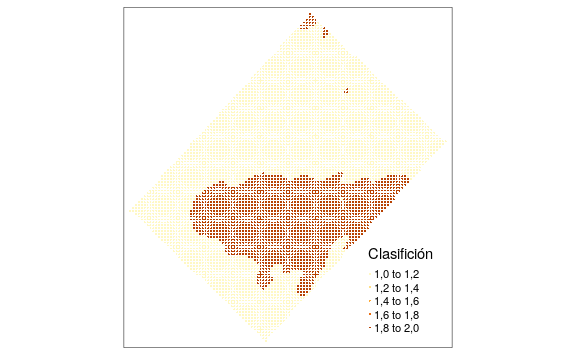
\includegraphics[width=\linewidth]{figuras/figLibro/tmapclasificacion-1} \end{center}

\hypertarget{predicciuxf3n-con-muxfaltiples-capas-de-datos-1}{%
\section{Predicción con múltiples capas de datos}\label{predicciuxf3n-con-muxfaltiples-capas-de-datos-1}}

En esta sección también se usa la base de datos \textbf{Pred2.txt} que contiene mediciones de conductividad eléctrica aparente en dos profundidades 0-30 cm (CE30) y 0-90 cm (CE90), elevación (Elev), profundidad de suelo (Pe) y rendimiento de trigo (Tg). La matriz de datos está conformada por n=482 sitios (filas) y p=7 variables (columnas).

Adicionalmente, para realizar la interpolación utilizando información de las covariables es necesario que la grilla de predicción contenga los valores de las coordenadas y de las covariables. El archivo \textbf{grilla\_am.txt} contiene estos datos. A continuación, se cargan ambas bases de datos y transforma a objetos de clase \texttt{sf}.

\begin{Shaded}
\begin{Highlighting}[]
\NormalTok{pred <-}\StringTok{ }\KeywordTok{read.table}\NormalTok{(}\StringTok{"datos/Pred2.txt"}\NormalTok{, }
                   \DataTypeTok{header =} \OtherTok{TRUE}\NormalTok{)}
\NormalTok{pred <-}\StringTok{ }\KeywordTok{st_as_sf}\NormalTok{(pred, }\DataTypeTok{coords =} \KeywordTok{c}\NormalTok{(}\StringTok{"x"}\NormalTok{, }\StringTok{"y"}\NormalTok{), }
                 \DataTypeTok{crs =} \DecValTok{32721}\NormalTok{)}
\KeywordTok{head}\NormalTok{(pred)}
\CommentTok{#> Simple feature collection with 6 features}
\NormalTok{and }\DecValTok{5}\NormalTok{ fields}
\CommentTok{#> geometry type: POINT}
\CommentTok{#> dimension: XY}
\CommentTok{#> bbox: xmin: 312000 ymin: 5800000 xmax:}
\DecValTok{312000}\NormalTok{ ymax}\OperatorTok{:}\StringTok{ }\DecValTok{5800000}
\CommentTok{#> epsg (SRID): 32721}
\CommentTok{#> proj4string: }
    \OperatorTok{+}\StringTok{ }\NormalTok{proj=utm }
    \OperatorTok{+}\StringTok{ }\NormalTok{zone=}\DecValTok{21} 
    \OperatorTok{+}\StringTok{ }\NormalTok{south}
\OperatorTok{+}\NormalTok{datum=WGS84 }\OperatorTok{+}\NormalTok{units=m }\OperatorTok{+}\NormalTok{no_defs}
\CommentTok{#> First 3 features:}
\CommentTok{#> Pe Elev CE30 CE90 Tg geometry}
\CommentTok{#> 1 80 161 21,8 30,6 4,19 POINT (312283}
\DecValTok{5800205}\ErrorTok{)}
\CommentTok{#> 2 40 161 30,3 17,9 4,00 POINT (312257}
\DecValTok{5800229}\ErrorTok{)}
\CommentTok{#> [ reached 'max'}
    \OperatorTok{/}\StringTok{ }\KeywordTok{getOption}\NormalTok{(}\StringTok{"max.print"}\NormalTok{) }\OperatorTok{--}
\NormalTok{omitted }\DecValTok{1}\NormalTok{ rows ]}
\NormalTok{grilla <-}\StringTok{ }\KeywordTok{read.table}\NormalTok{(}\StringTok{"datos/grilla_am.txt"}\NormalTok{, }
                     \DataTypeTok{header =} \OtherTok{TRUE}\NormalTok{)}
\NormalTok{grilla <-}\StringTok{ }\KeywordTok{st_as_sf}\NormalTok{(pred, }\DataTypeTok{coords =} \KeywordTok{c}\NormalTok{(}\StringTok{"x"}\NormalTok{, }\StringTok{"y"}\NormalTok{), }
                   \DataTypeTok{crs =} \DecValTok{32721}\NormalTok{)}
\end{Highlighting}
\end{Shaded}

\hypertarget{kriging-con-deriva-externa}{%
\subsection{Kriging con deriva externa}\label{kriging-con-deriva-externa}}

En las siguientes líneas de se realiza el ajuste del semivariograma empírico contemplando una tendencia dada por las covariables CE30, CE90, Elev y Pe y se realiza el ajuste de semivariogramas teóricos. Finalmente, se grafican ambos semivariogramas. Los resultados muestran que el modelo de mejor ajuste fue el exponencial. Los parámetros obtenidos fueron nugget (\(C_0=0.16\)), sill parcial (\(C=0.55\)) y rango (80 m). Nota: bajo la columna ``psill'', para la fila Nugget, se debe leer el valor \(C_0\).

\begin{Shaded}
\begin{Highlighting}[]
\NormalTok{semiv_ked <-}\StringTok{ }\KeywordTok{variogram}\NormalTok{(}
\NormalTok{  Tg }\OperatorTok{~}\StringTok{ }\NormalTok{CE30 }\OperatorTok{+}\StringTok{ }\NormalTok{CE90 }\OperatorTok{+}\StringTok{ }\NormalTok{Elev }\OperatorTok{+}\StringTok{ }\NormalTok{Pe, pred}
\NormalTok{  )}
\NormalTok{v.fit_vut_ked <-}\StringTok{ }
\StringTok{  }\KeywordTok{fit.variogram}\NormalTok{(semiv_ked , }
                \KeywordTok{vgm}\NormalTok{(}\KeywordTok{c}\NormalTok{(}\StringTok{"Exp"}\NormalTok{, }\StringTok{"Sph"}\NormalTok{, }\StringTok{"Gau"}\NormalTok{)))}
                               
\NormalTok{v.fit_vut_ked}
\CommentTok{#>   model psill range}
\CommentTok{#> 1   Nug 0,163   0,0}
\CommentTok{#> 2   Exp 0,549  80,7}
\KeywordTok{plot}\NormalTok{(semiv_ked , v.fit_vut_ked)}
\end{Highlighting}
\end{Shaded}

\begin{center}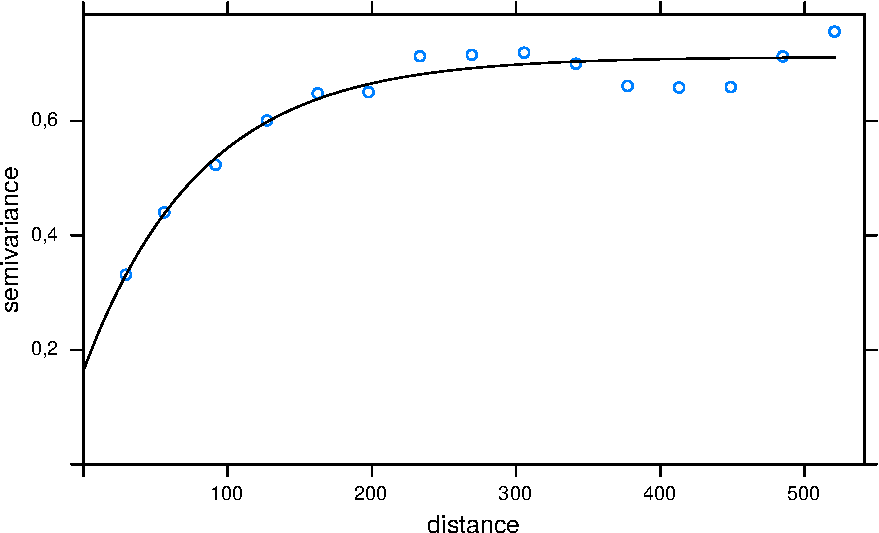
\includegraphics[width=\linewidth]{figuras/figLibro/unnamed-chunk-88-1} \end{center}

Para realizar la interpolación espacial se utiliza también la función \texttt{krige()} y se especifica la tendencia con las covariables en la fórmula. En este caso la predicción se realiza también en un contexto local (argumentos \texttt{nmin} y \texttt{nmax}).

\begin{Shaded}
\begin{Highlighting}[]
\NormalTok{kriging_ed <-}\StringTok{ }\KeywordTok{krige}\NormalTok{(}
\NormalTok{  Tg }\OperatorTok{~}\StringTok{ }\NormalTok{CE30 }\OperatorTok{+}\StringTok{ }\NormalTok{CE90 }\OperatorTok{+}\StringTok{ }\NormalTok{Elev }\OperatorTok{+}\StringTok{ }\NormalTok{Pe,}
\NormalTok{  pred,}
\NormalTok{  grilla,}
  \DataTypeTok{model =}\NormalTok{ v.fit_vut_ked,}
  \DataTypeTok{nmin =} \DecValTok{7}\NormalTok{,}
  \DataTypeTok{nmax =} \DecValTok{25}
\NormalTok{)}
\CommentTok{#> [using universal kriging]}
\end{Highlighting}
\end{Shaded}

\begin{Shaded}
\begin{Highlighting}[]

\NormalTok{prediccionKED <-}
\StringTok{  }\KeywordTok{tm_shape}\NormalTok{(kriging_ed) }\OperatorTok{+}
\StringTok{  }\KeywordTok{tm_dots}\NormalTok{(}\StringTok{"var1.pred"}\NormalTok{, }\DataTypeTok{style =} \StringTok{"cont"}\NormalTok{,}
          \DataTypeTok{title =} \StringTok{"Predicción KED"}\NormalTok{)}

\NormalTok{varianzaKED <-}
\StringTok{  }\KeywordTok{tm_shape}\NormalTok{(kriging_o) }\OperatorTok{+}
\StringTok{  }\KeywordTok{tm_dots}\NormalTok{(}\StringTok{"var1.var"}\NormalTok{, }\DataTypeTok{style =} \StringTok{"cont"}\NormalTok{,}
          \DataTypeTok{title =} \StringTok{"Varianza KED"}\NormalTok{) }

\KeywordTok{tmap_arrange}\NormalTok{(prediccionKED, varianzaKED)}
\end{Highlighting}
\end{Shaded}

\begin{center}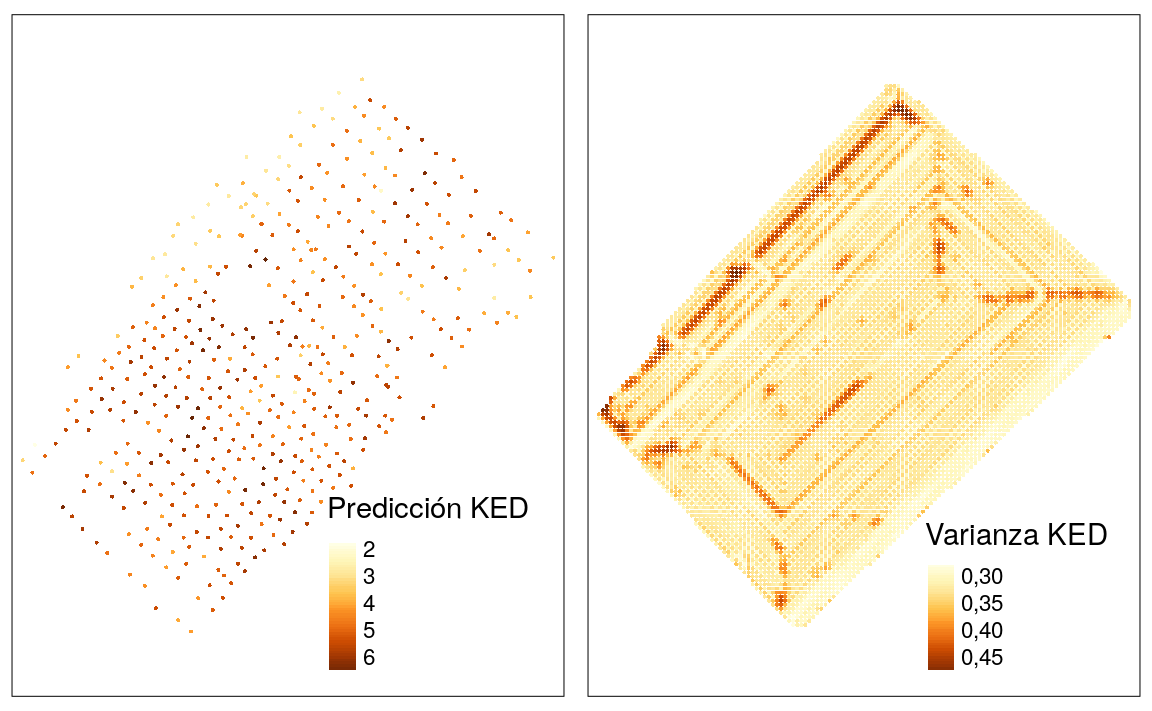
\includegraphics[width=\linewidth]{figuras/figLibro/tmapKED-1} \end{center}

\hypertarget{kriging-desde-modelo-de-regresiuxf3n}{%
\subsection{Kriging desde modelo de regresión}\label{kriging-desde-modelo-de-regresiuxf3n}}

Para realizar la interpolación por el método kriging regresión primero se ajusta un modelo lineal de regresión entre la variable Tg y las covariables CE30, CE90, Elev y Pe.

\begin{Shaded}
\begin{Highlighting}[]
\NormalTok{mlr <-}\StringTok{ }\KeywordTok{lm}\NormalTok{(Tg }\OperatorTok{~}\StringTok{ }\NormalTok{CE30 }\OperatorTok{+}\StringTok{ }\NormalTok{CE90 }\OperatorTok{+}\StringTok{ }\NormalTok{Elev }\OperatorTok{+}\StringTok{ }\NormalTok{Pe, pred)}
\end{Highlighting}
\end{Shaded}

A partir del modelo ajustado se obtienen los residuos que son incorporados al objeto \texttt{pred}. Luego sobre estos residuos se modela el semivariograma empírico y teórico. Los resultados muestran que los valores estimados de los parámetros del semivariograma son similares a los obtenidos en el caso anterior. Esto es esperable ya que ambas aproximaciones son equivalentes.

\begin{Shaded}
\begin{Highlighting}[]
\NormalTok{pred}\OperatorTok{$}\NormalTok{residuos <-}\StringTok{ }\NormalTok{mlr}\OperatorTok{$}\NormalTok{residuals}
\KeywordTok{names}\NormalTok{(pred)}
\CommentTok{#> [1] "Pe" "Elev" "CE30" "CE90" "Tg"}
\StringTok{"geometry"} \StringTok{"residuos"}
\end{Highlighting}
\end{Shaded}

\begin{Shaded}
\begin{Highlighting}[]
\NormalTok{semiv_rk <-}\StringTok{ }\KeywordTok{variogram}\NormalTok{(residuos }\OperatorTok{~}\StringTok{ }\DecValTok{1}\NormalTok{ , pred)}

\NormalTok{v.fit_vut_rk <-}\StringTok{ }
\StringTok{  }\KeywordTok{fit.variogram}\NormalTok{(semiv_rk , }
                \KeywordTok{vgm}\NormalTok{(}\KeywordTok{c}\NormalTok{(}\StringTok{"Exp"}\NormalTok{, }\StringTok{"Sph"}\NormalTok{, }\StringTok{"Gau"}\NormalTok{)))}
\NormalTok{v.fit_vut_rk}
\CommentTok{#>   model psill range}
\CommentTok{#> 1   Nug 0,163   0,0}
\CommentTok{#> 2   Exp 0,549  80,7}
\end{Highlighting}
\end{Shaded}

\begin{Shaded}
\begin{Highlighting}[]
\KeywordTok{plot}\NormalTok{(semiv_rk , v.fit_vut_rk)}
\end{Highlighting}
\end{Shaded}

\begin{center}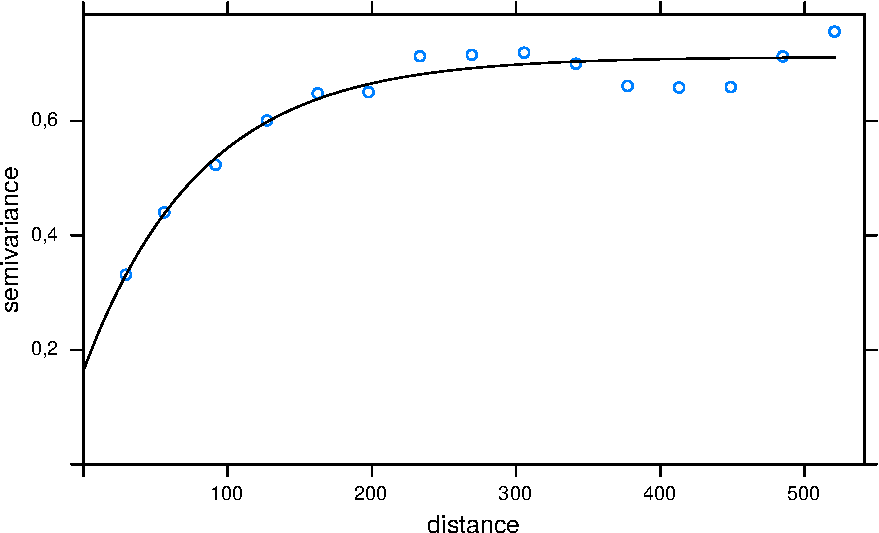
\includegraphics[width=\linewidth]{figuras/figLibro/unnamed-chunk-93-1} \end{center}

Finalmente se realiza la predicción en la grilla de los residuos y esta es sumada a la predicción del modelo de regresión ajustado inicialmente para obtener los valores predichos finales.

\begin{Shaded}
\begin{Highlighting}[]
\NormalTok{kgres <-}\StringTok{ }\KeywordTok{krige}\NormalTok{(residuos }\OperatorTok{~}\StringTok{ }\DecValTok{1}\NormalTok{, pred, }
\NormalTok{               grilla, }\DataTypeTok{model =}\NormalTok{ v.fit_vut_rk)}
\CommentTok{#> [using ordinary kriging]}
\NormalTok{grilla}\OperatorTok{$}\NormalTok{RK_pred <-}\StringTok{ }
\StringTok{  }\KeywordTok{predict}\NormalTok{(mlr, }\DataTypeTok{newdata =}\NormalTok{ grilla) }\OperatorTok{+}\StringTok{ }
\StringTok{  }\NormalTok{kgres}\OperatorTok{$}\NormalTok{var1.pred}
\end{Highlighting}
\end{Shaded}

\begin{Shaded}
\begin{Highlighting}[]

\KeywordTok{tm_shape}\NormalTok{(grilla) }\OperatorTok{+}
\StringTok{  }\KeywordTok{tm_dots}\NormalTok{(}\StringTok{"RK_pred"}\NormalTok{, }\DataTypeTok{style =} \StringTok{"cont"}\NormalTok{,}
          \DataTypeTok{title =} \StringTok{"Predicción RK"}\NormalTok{)}
\end{Highlighting}
\end{Shaded}

\begin{center}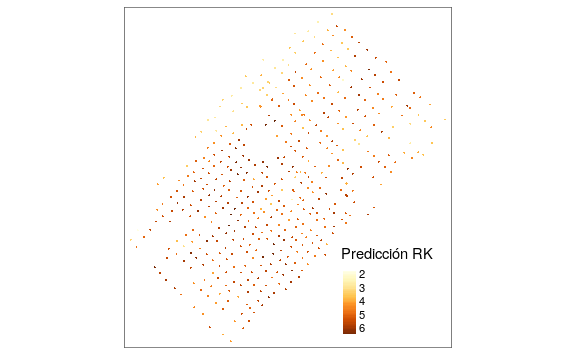
\includegraphics[width=\linewidth]{figuras/figLibro/tmapRK-1} \end{center}

\hypertarget{uxe1rboles-aleatorios}{%
\subsection{Árboles aleatorios}\label{uxe1rboles-aleatorios}}

Para este método primero se ajusta el algoritmo \emph{random forest} utilizando para ello el paquete \texttt{caret}. Para ello se optimizará el parámetro \texttt{mtry} mediante un proceso de validación cruzada. Los valores prbados de \texttt{mtry} se especifican en el objeto que lleva el mismo nombre. Con la función \texttt{fitControl()} se estable el tipo de validación cruzada, en este caso k-fold con k=10. Además, se permite el paralelizado del proceso en caso de ser necesario (\texttt{allowParallel=T}).

\begin{Shaded}
\begin{Highlighting}[]
\NormalTok{mtry <-}\StringTok{ }\KeywordTok{expand.grid}\NormalTok{(}\DataTypeTok{mtry =} \KeywordTok{seq}\NormalTok{(}\DecValTok{1}\NormalTok{, }\DecValTok{4}\NormalTok{, }\DecValTok{1}\NormalTok{))}
\NormalTok{fitControl <-}\StringTok{ }\KeywordTok{trainControl}\NormalTok{(}\DataTypeTok{method =} \StringTok{"cv"}\NormalTok{,}
                           \DataTypeTok{number =} \DecValTok{10}\NormalTok{,}
                           \DataTypeTok{allowParallel =}\NormalTok{ T)}
\end{Highlighting}
\end{Shaded}

Las siguientes son las opciones de paralelizado que involucra los paquetes \texttt{parallel} y \texttt{doParallel}

\begin{Shaded}
\begin{Highlighting}[]
\KeywordTok{library}\NormalTok{(parallel)}
\KeywordTok{library}\NormalTok{(doParallel)}
\NormalTok{cluster <-}\StringTok{ }\KeywordTok{makeCluster}\NormalTok{(}\KeywordTok{max}\NormalTok{(}\DecValTok{1}\NormalTok{, }\KeywordTok{detectCores}\NormalTok{() }\OperatorTok{-}\StringTok{ }\DecValTok{1}\NormalTok{))}
\KeywordTok{registerDoParallel}\NormalTok{(cluster)}
\end{Highlighting}
\end{Shaded}

El ajuste del \emph{random forest} se realiza con la función \texttt{train()} la cual requiere entre otros especifica la fórmula o modelo, la base de datos a utilizar, el algoritmo (\texttt{rf}, random forest), grilla de valores de hiperparámetros a evaluar (objeto \texttt{mtry}) y opciones de la validación.

\begin{Shaded}
\begin{Highlighting}[]
\KeywordTok{set.seed}\NormalTok{(}\DecValTok{7}\NormalTok{)}
\NormalTok{train_rf <-}\StringTok{ }\KeywordTok{train}\NormalTok{(}
\NormalTok{  Tg }\OperatorTok{~}\StringTok{ }\NormalTok{CE30 }\OperatorTok{+}\StringTok{ }\NormalTok{CE90 }\OperatorTok{+}\StringTok{ }\NormalTok{Elev }\OperatorTok{+}\StringTok{ }\NormalTok{Pe,}
  \DataTypeTok{data =}\NormalTok{ pred,}
  \DataTypeTok{method =} \StringTok{"rf"}\NormalTok{,}
  \DataTypeTok{tuneGrid =}\NormalTok{ mtry,}
  \DataTypeTok{trControl =}\NormalTok{ fitControl}
\NormalTok{)}
\end{Highlighting}
\end{Shaded}

Luego de ajustar el modelo de RF se procede a obtener los residuos y el ajuste de los semivariogramas.

\begin{Shaded}
\begin{Highlighting}[]
\NormalTok{pred}\OperatorTok{$}\NormalTok{residuosRF <-}\StringTok{ }
\StringTok{  }\NormalTok{pred}\OperatorTok{$}\NormalTok{Tg }\OperatorTok{-}\StringTok{ }\KeywordTok{predict}\NormalTok{(train_rf, }\DataTypeTok{newdata =}\NormalTok{ pred)}

\NormalTok{semiv_RFk <-}\StringTok{ }\KeywordTok{variogram}\NormalTok{(residuosRF }\OperatorTok{~}\StringTok{ }\DecValTok{1}\NormalTok{ , pred)}
\KeywordTok{plot}\NormalTok{(semiv_RFk)}

\NormalTok{v.fit_vut_RFk <-}\StringTok{ }
\StringTok{  }\KeywordTok{fit.variogram}\NormalTok{(semiv_RFk , }
                \KeywordTok{vgm}\NormalTok{(}\KeywordTok{c}\NormalTok{(}\StringTok{"Exp"}\NormalTok{, }\StringTok{"Sph"}\NormalTok{, }\StringTok{"Gau"}\NormalTok{)))}
\KeywordTok{plot}\NormalTok{(semiv_RFk , v.fit_vut_RFk)}
\end{Highlighting}
\end{Shaded}

\begin{center}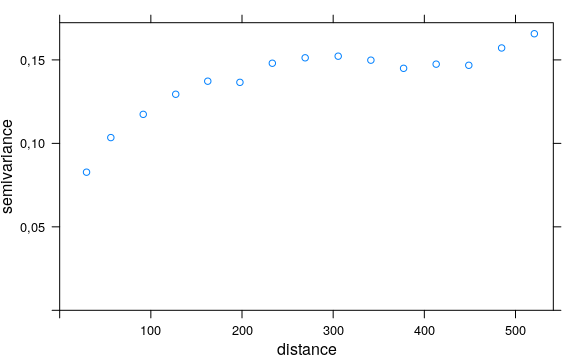
\includegraphics[width=\linewidth]{figuras/figLibro/unnamed-chunk-98-1} 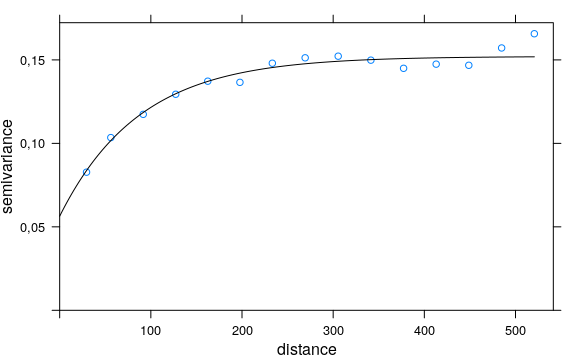
\includegraphics[width=\linewidth]{figuras/figLibro/unnamed-chunk-98-2} \end{center}

Finalmente se realiza la predicción de los residuos sobre la grilla y se suman a la predicción del modelo de random forest ajustado inicialmente.

\begin{Shaded}
\begin{Highlighting}[]
\NormalTok{kgresRF <-}\StringTok{ }\KeywordTok{krige}\NormalTok{(residuosRF }\OperatorTok{~}\StringTok{ }\DecValTok{1}\NormalTok{, pred, }
\NormalTok{                 grilla, }\DataTypeTok{model =}\NormalTok{ v.fit_vut_RFk)}
\CommentTok{#> [using ordinary kriging]}
\end{Highlighting}
\end{Shaded}

\begin{Shaded}
\begin{Highlighting}[]

\KeywordTok{tm_shape}\NormalTok{(grilla) }\OperatorTok{+}
\StringTok{  }\KeywordTok{tm_dots}\NormalTok{(}\StringTok{"RK_pred"}\NormalTok{, }\DataTypeTok{style =} \StringTok{"cont"}\NormalTok{,}
          \DataTypeTok{title =} \StringTok{"Predicción RFK"}\NormalTok{) }
\end{Highlighting}
\end{Shaded}

\begin{center}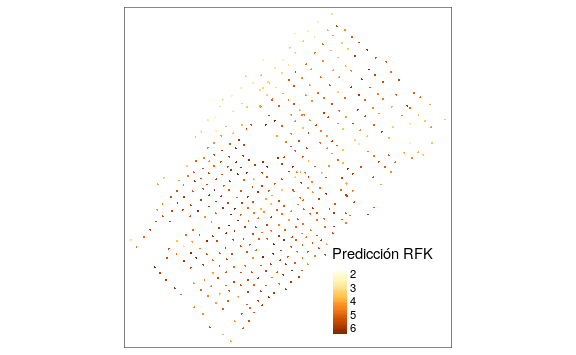
\includegraphics[width=\linewidth]{figuras/figLibro/tmapRFK-1} \end{center}

\hypertarget{implementaciuxf3n-con-infostat}{%
\chapter{Implementación con InfoStat}\label{implementaciuxf3n-con-infostat}}

El módulo ``Estadística Espacial'' de InfoStat permite realizar, a través de su conexión con el software R, la implementación de algoritmos univariados y multivariados para el análisis de datos georreferenciados. En esta sección se ilustrará el uso de este módulo para la transformación de coordenadas, la depuración de datos georreferenciados, el cálculo de índices de autocorrelación espacial, ajuste de semivariogramas, y la obtención de un mapa de variabilidad espacial mediante interpolación kriging. Complementariamente, se ilustra su aplicación con bases de datos de naturaleza multivariada para el cálculo de correlación bivariada, la implementación del análisis de componentes principales espaciales (MULTISPATI-PCA), la clasificación KM-sPC y el uso de métodos de regresión basados en árboles (\emph{Random Forest}).

\hypertarget{conversiuxf3n-de-coordenadas-espaciales-1}{%
\section{Conversión de coordenadas espaciales}\label{conversiuxf3n-de-coordenadas-espaciales-1}}

Este menú permite la conversión entre distintos sistemas de coordenadas de referencias basándose en el uso de los códigos EPSG (\url{http://www.epsg.org/}). El archivo de datos que se abre desde el menú Aplicaciones \(\to\) Estadística Espacial \(\to\) Transformación de Coordenadas \(\to\) Datos de prueba. El archivo se denomina \textbf{datosRinde.idb2} y contiene 9810 observaciones (registros o filas del archivo) sobre datos de rendimiento de trigo (Rinde, \(t\ ha^{-1}\)) de un lote agrícola que fueron recolectados con un monitor de rendimiento. Cada valor registrado posee su ubicación geográfica (x e y) en unidades grado decimal que son expresadas en longitud (x) y latitud (y).

\begin{center}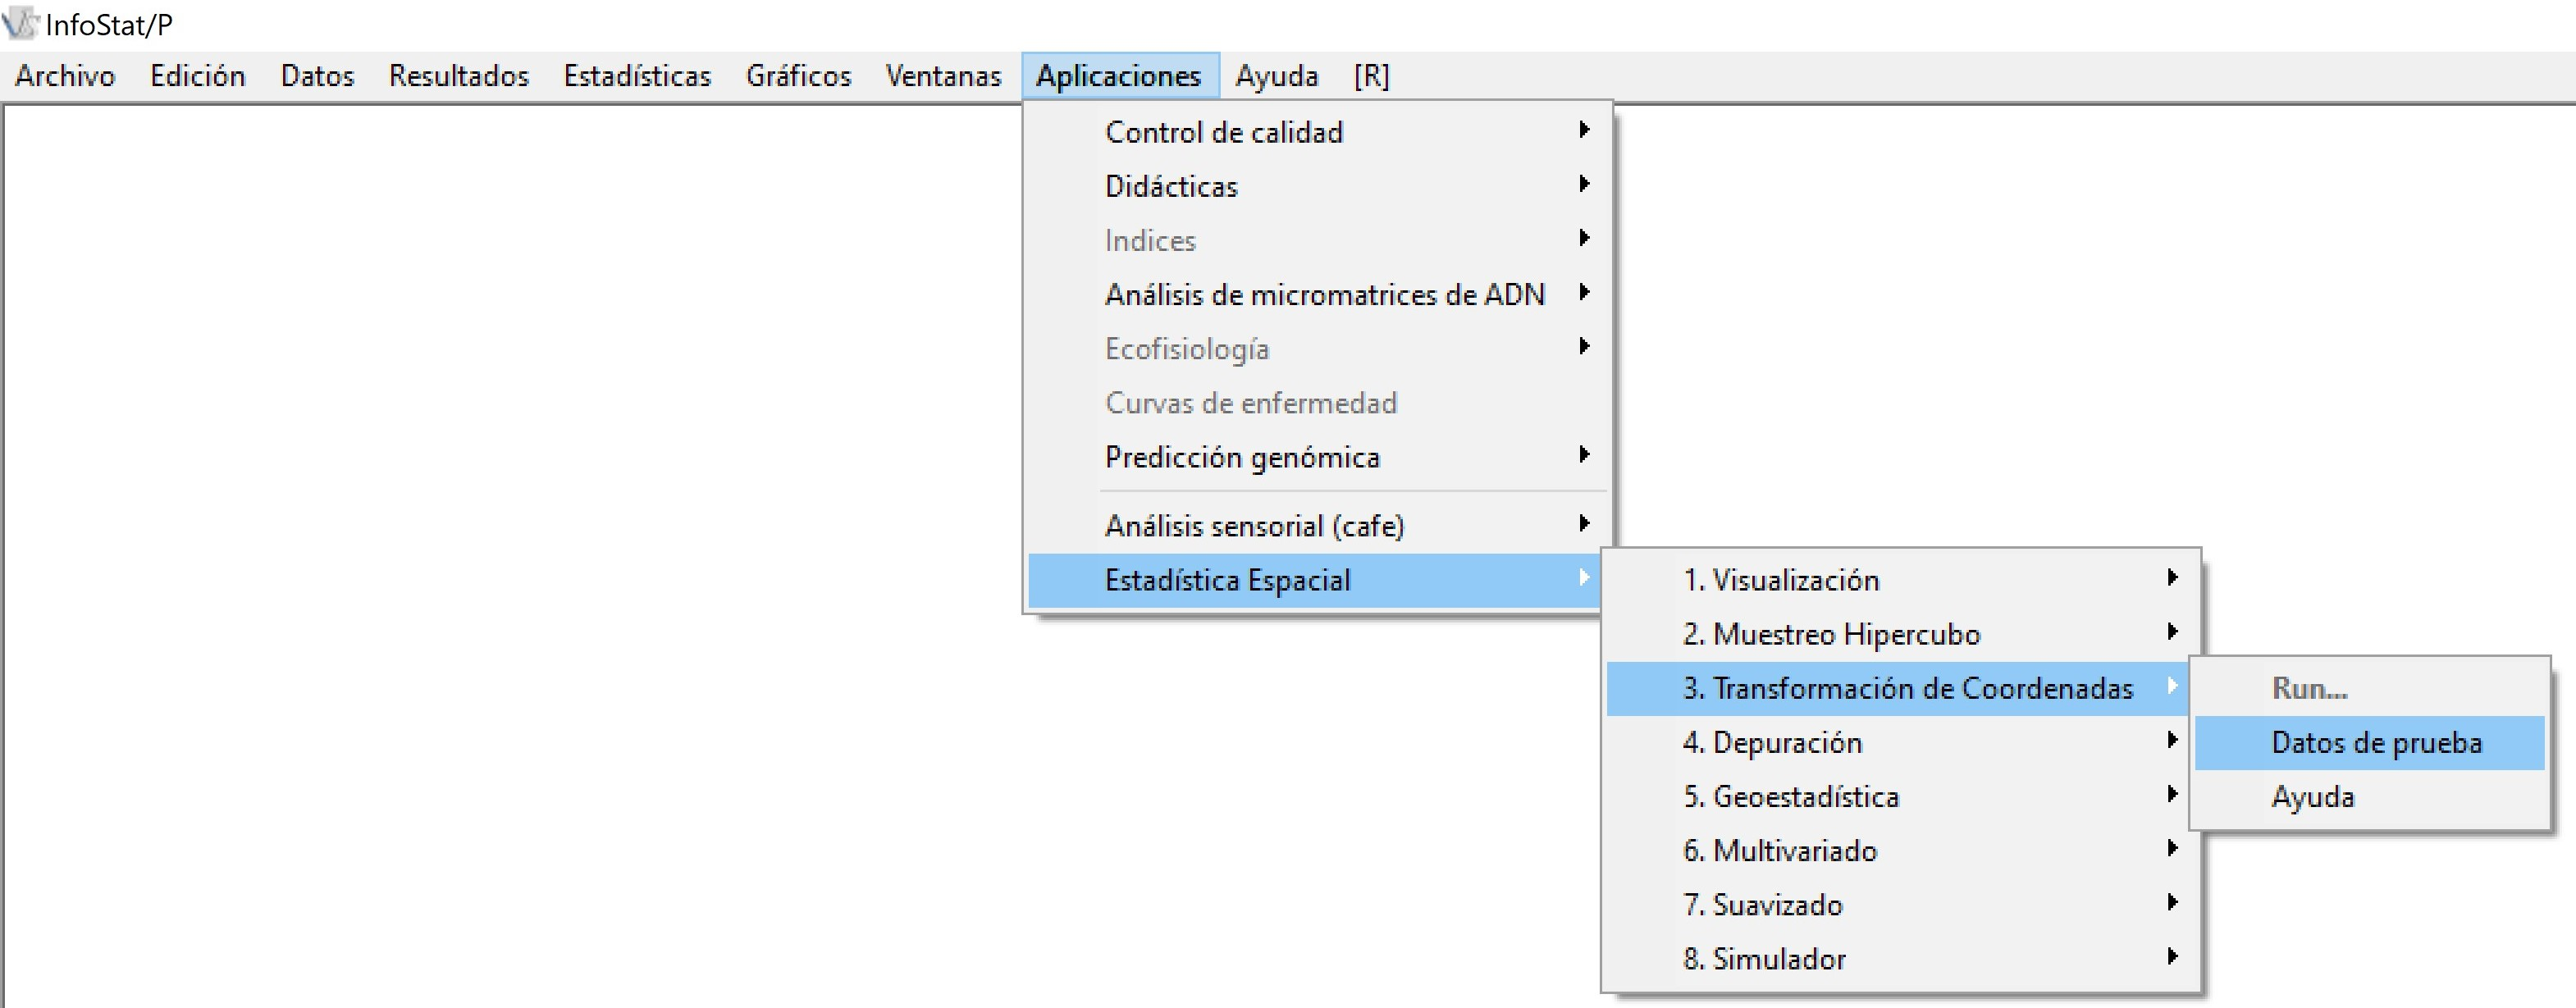
\includegraphics[width=\linewidth]{figuras/Parte2/1} \end{center}

\begin{center}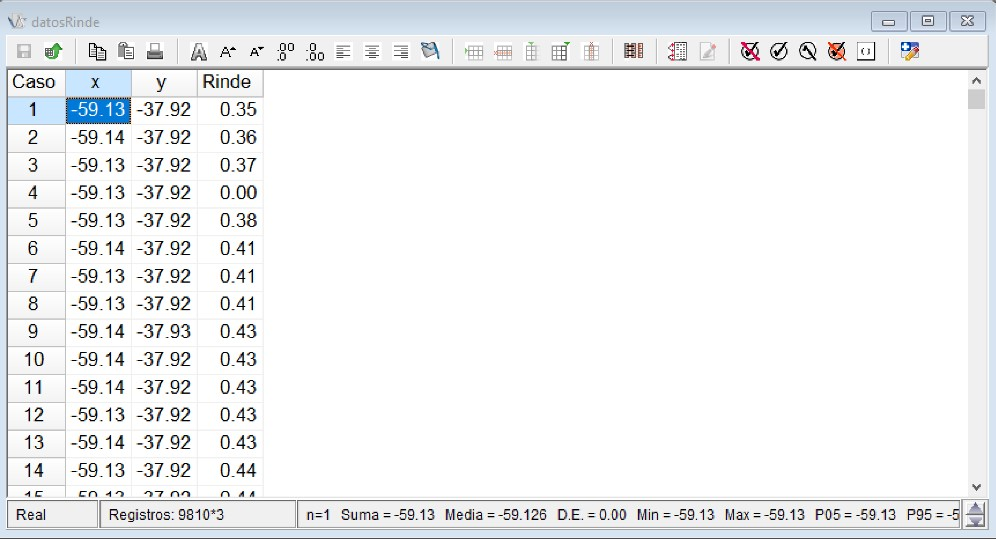
\includegraphics[width=\linewidth]{figuras/Parte2/2} \end{center}

En el menú Aplicaciones \(\to\) Estadística Espacial \(\to\) Transformación de Coordenadas \(\to\) Run, se abrirá una ventana de selector de variables donde debe indicarse la columna del archivo de datos que contiene la información correspondiente a la Coordenada X y la columna del archivo que contiene la información de la Coordenada Y. Luego, aparecerá una ventana para seleccionar el código EPSG original de los datos y código asignado. En este ejemplo el código original para las coordenadas geográficas WGS84 es 4326 y el asignado para el sistema UTM zona 21 es 32721. En caso de ser necesario previo a esta transformación permite también el pasaje de datos que estén expresados en grados, minutos y segundos a grados decimales. Para ello sólo se debe tildar esta opción en el cuadro de dialogo. Los valores de las coordenadas deben presentarse con un espacio entre subunidades. Por ejemplo ``33 1 1'' expresan los grados minutos y segundos respectivamente.

\begin{center}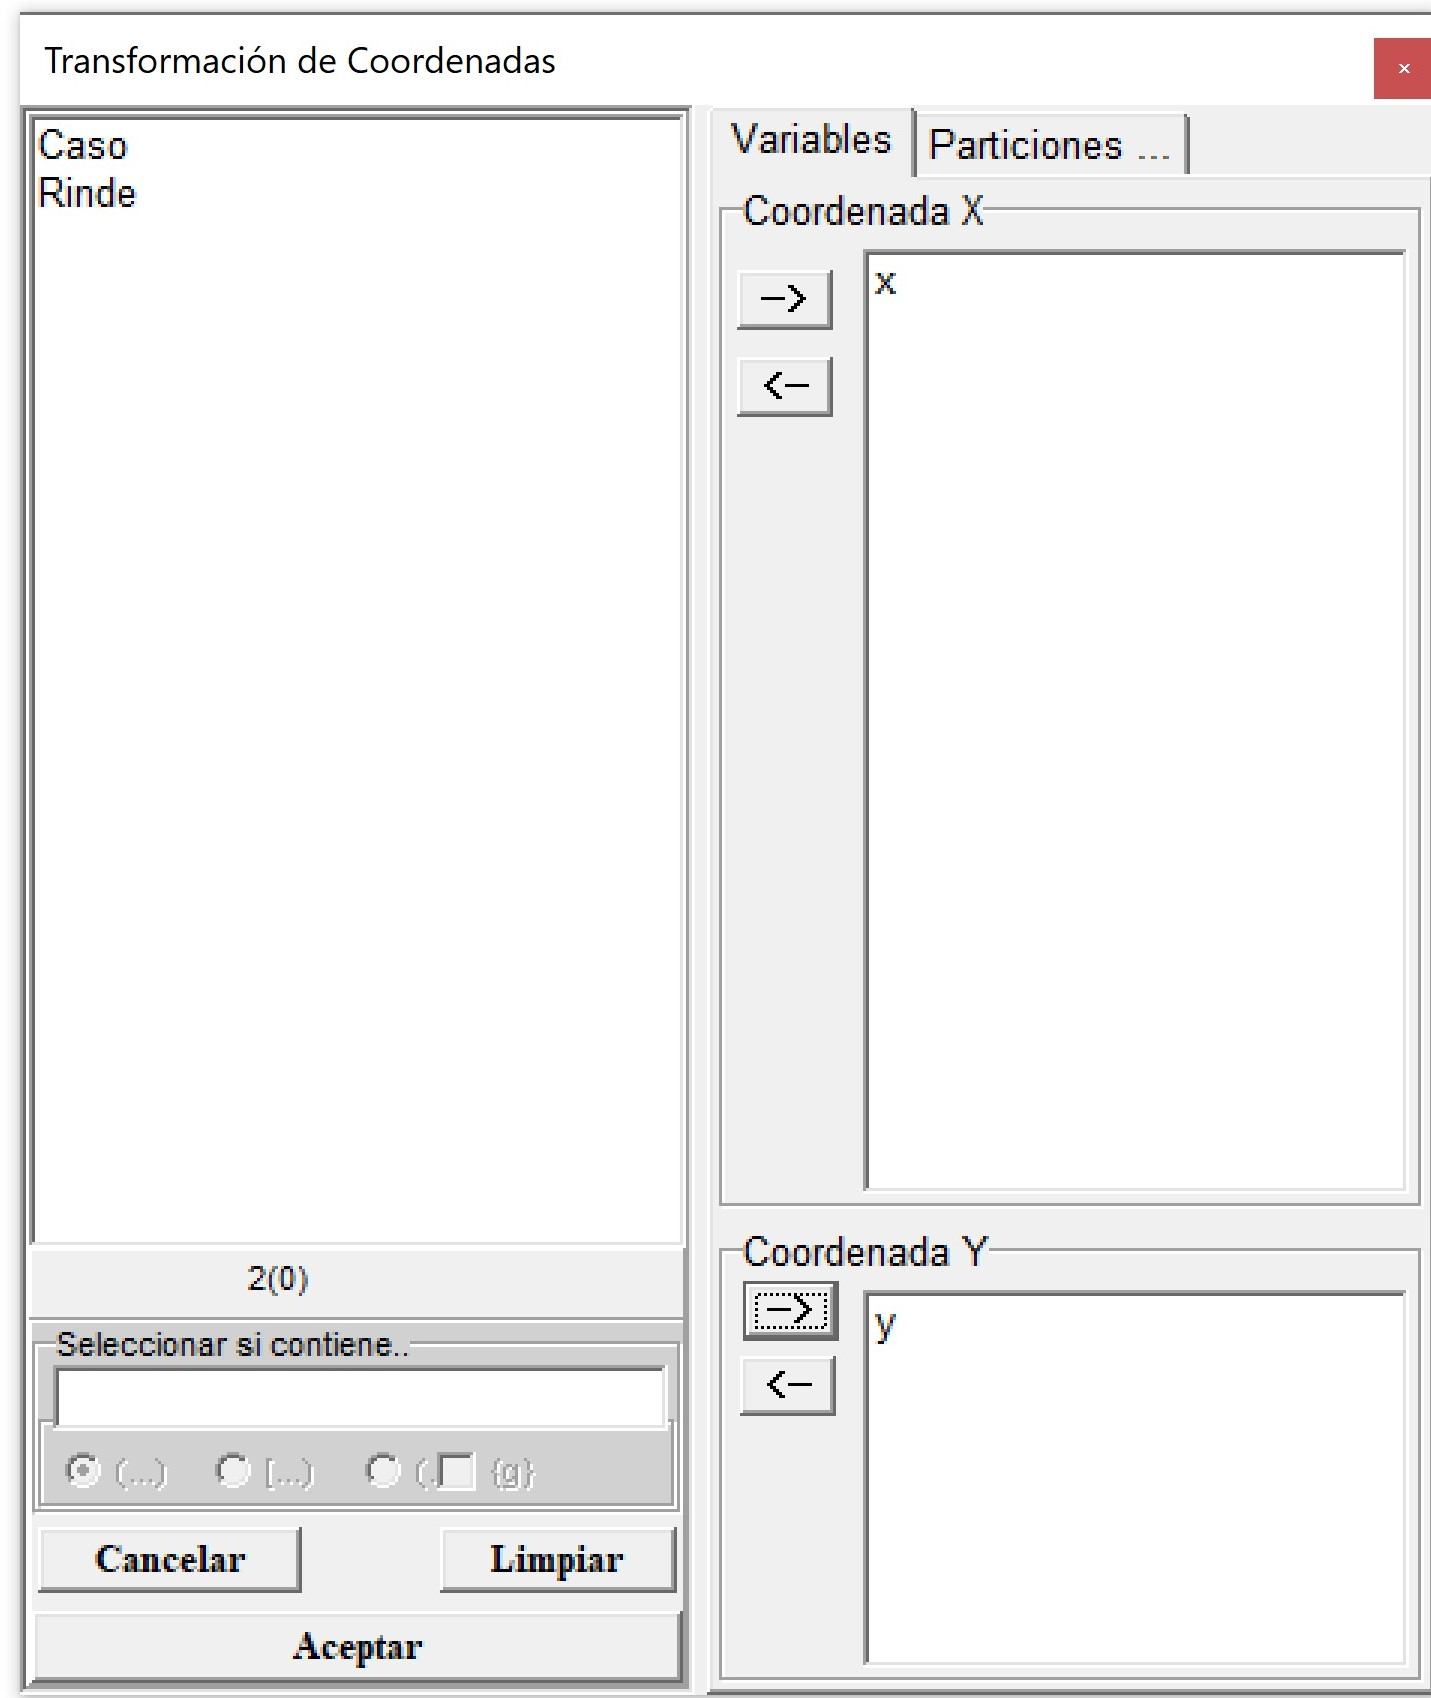
\includegraphics[width=0.7\linewidth]{figuras/Parte2/3} \end{center}

\begin{center}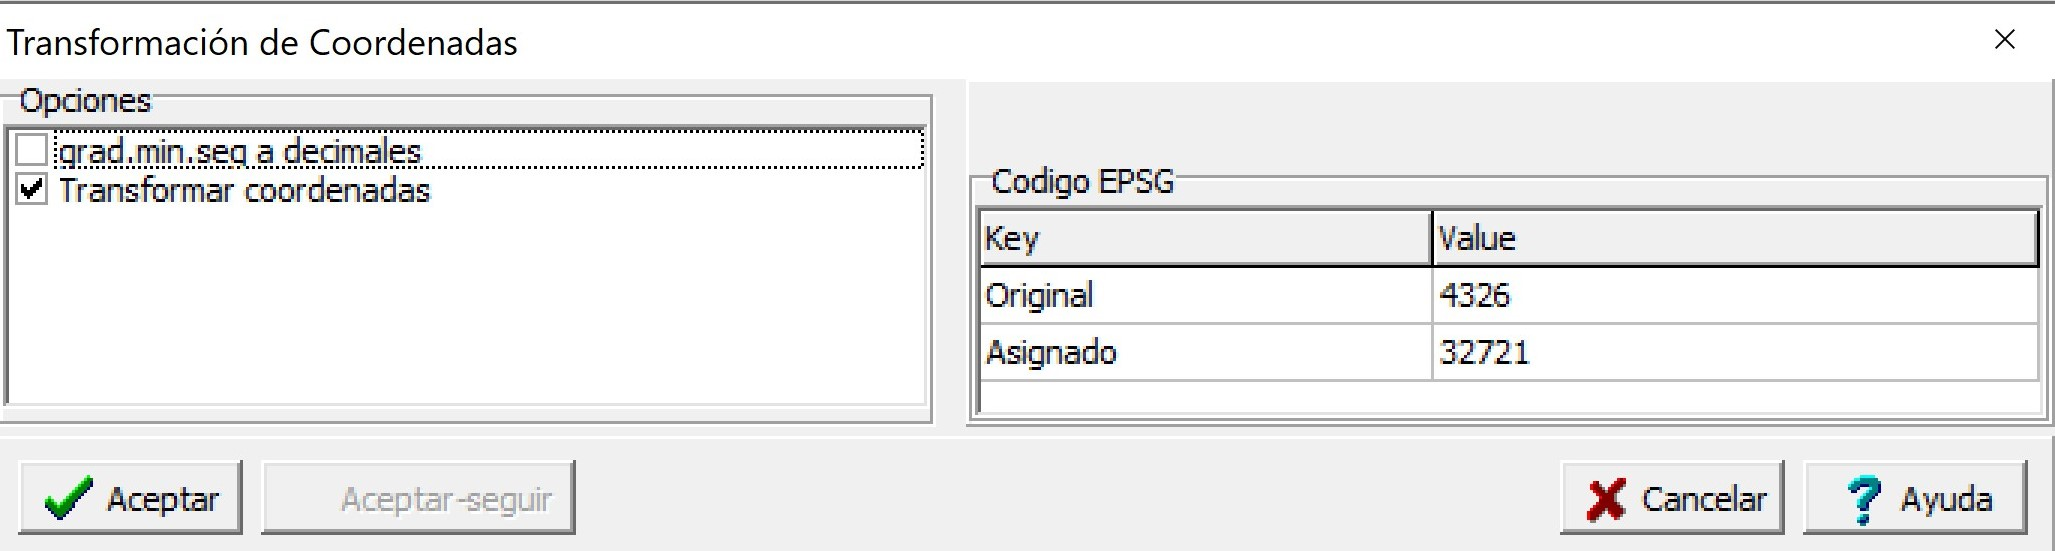
\includegraphics[width=\linewidth]{figuras/Parte2/4} \end{center}

Como resultado, en la tabla de datos original se agregarán dos nuevas columnas, al final del archivo, correspondiente a las coordenadas x e y transformadas, las cuales se denominarán Xt e Yt, haciendo referencia a la variable x transformada (Xt) y a la variable y transformada (Yt). Estas nuevas variables (coordenadas transformadas) permiten interpretar la distancia entre puntos de Rinde en metros.

\begin{center}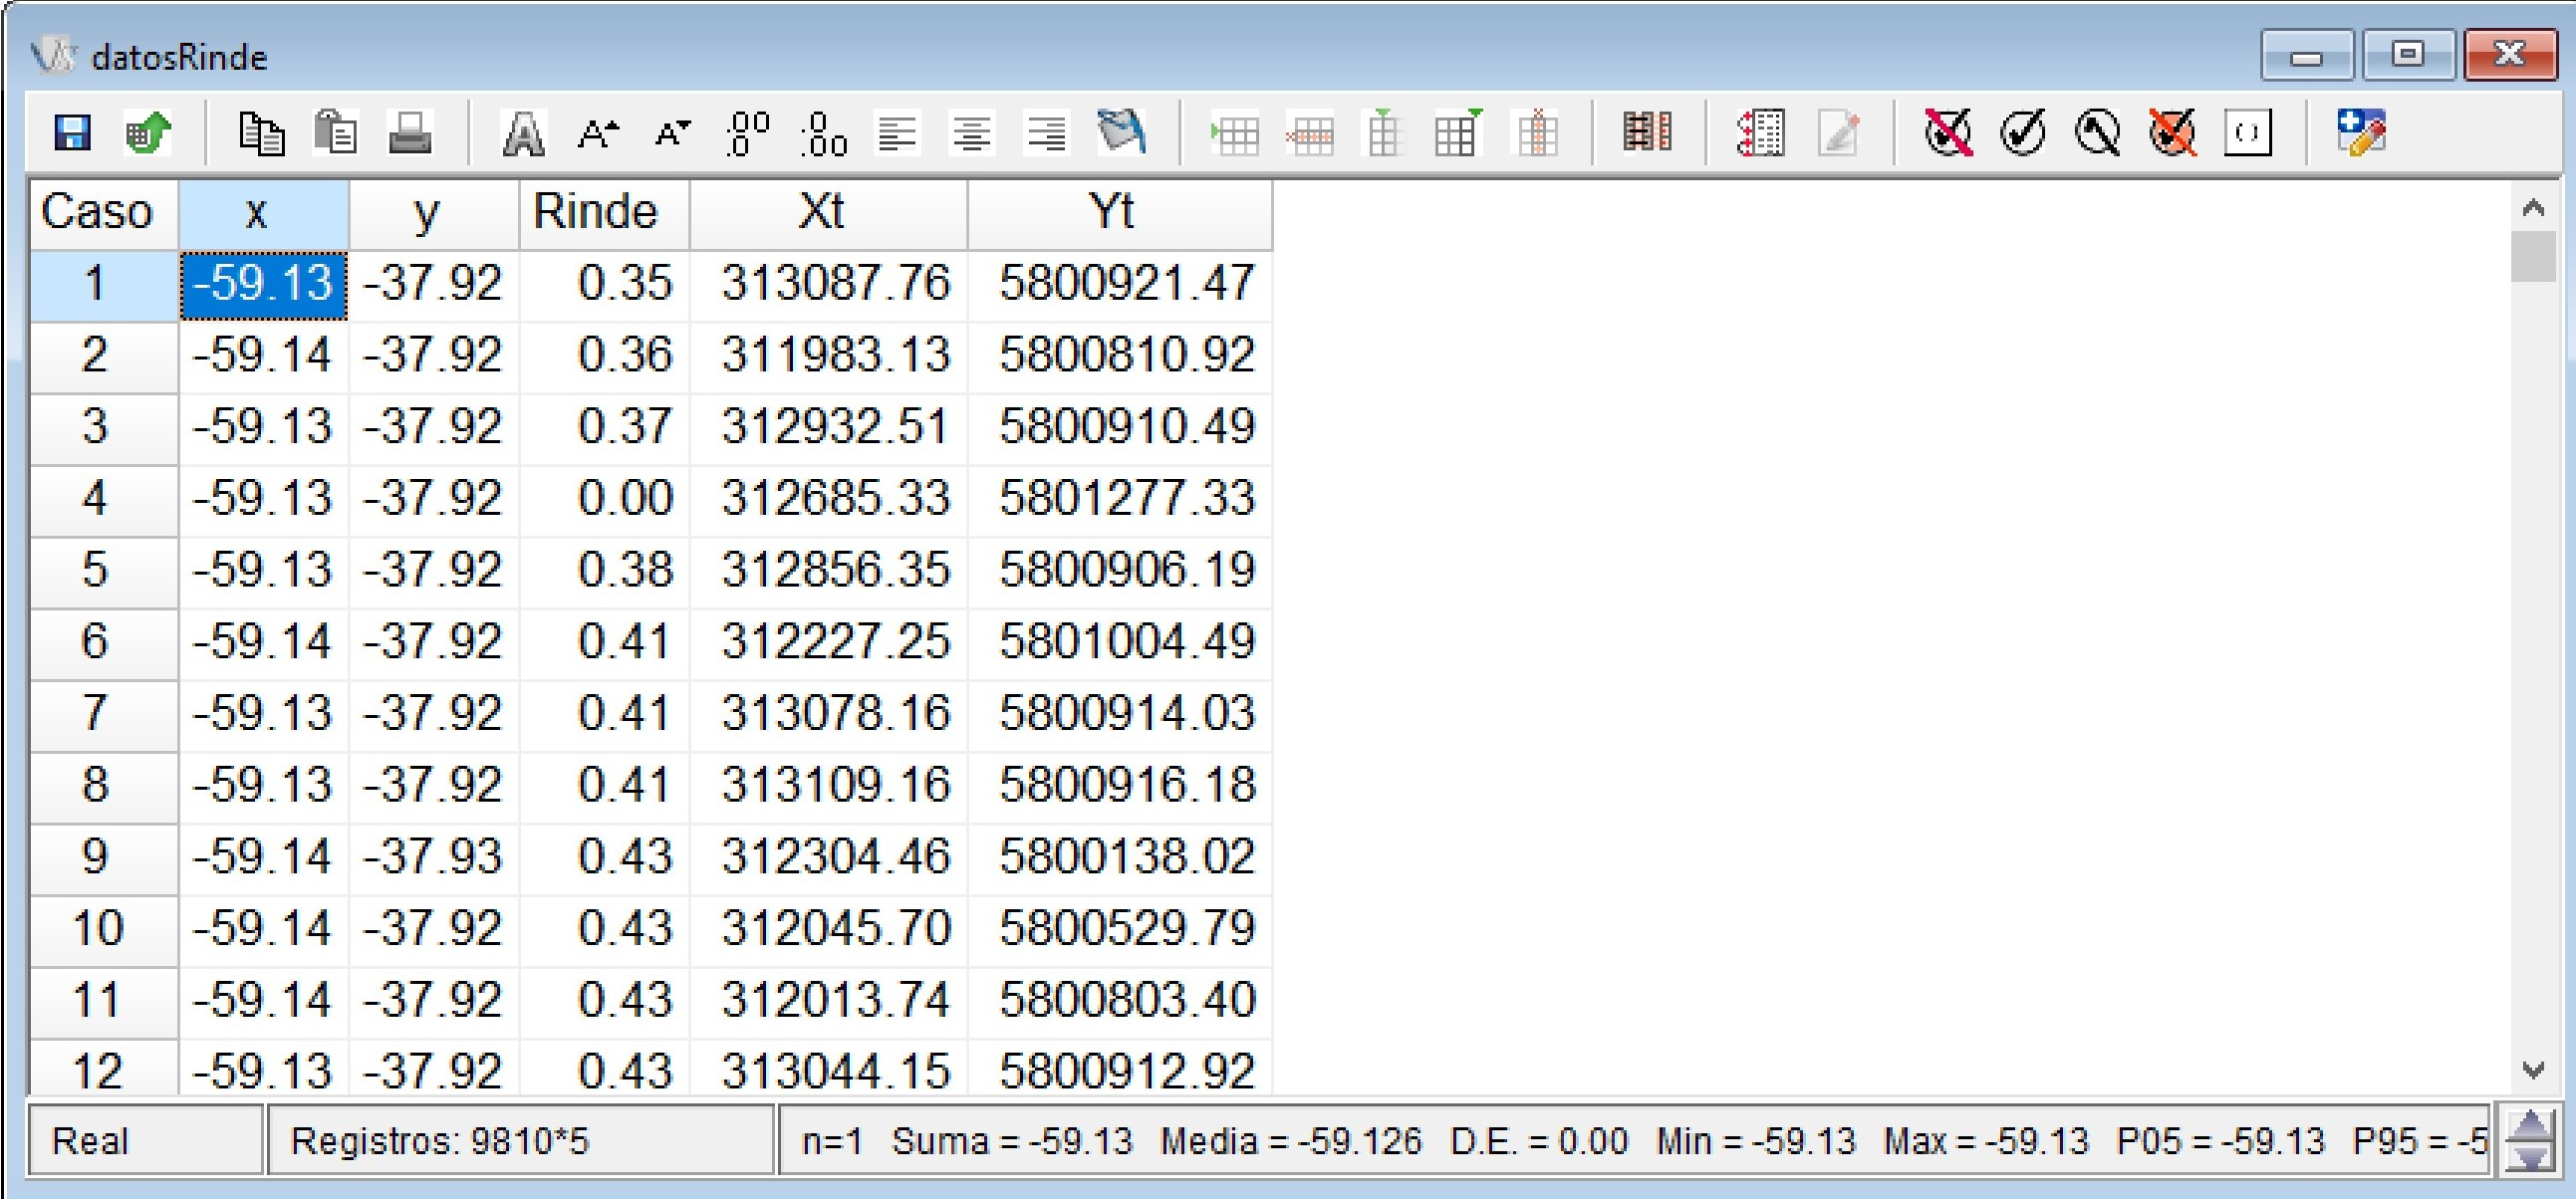
\includegraphics[width=\linewidth]{figuras/Parte2/5} \end{center}

\hypertarget{eliminaciuxf3n-de-outliers-e-inliers-1}{%
\section{\texorpdfstring{Eliminación de \emph{outliers} e \emph{inliers}}{Eliminación de outliers e inliers}}\label{eliminaciuxf3n-de-outliers-e-inliers-1}}

En el menú Aplicaciones \(\to\) Estadística Espacial \(\to\) Depuración \(\to\) Datos de prueba se abrirá un archivo denominado \textbf{datosRinde\_t.idb2} con 9810 registros y tres columnas correspondientes a las coordenadas planas UTM (x e y) de cada observación y los valores de la variable rendimiento de trigo (\(t\ ha^{-1}\)). Luego, en el menú Aplicaciones \(\to\) Estadística Espacial \(\to\) Depuración \(\to\) Run, se selecciona la variable respuesta, en este ejemplo Rinde y las columnas que indican la ubicación espacial de cada observación en el cuadro de Coordenadas.

\begin{center}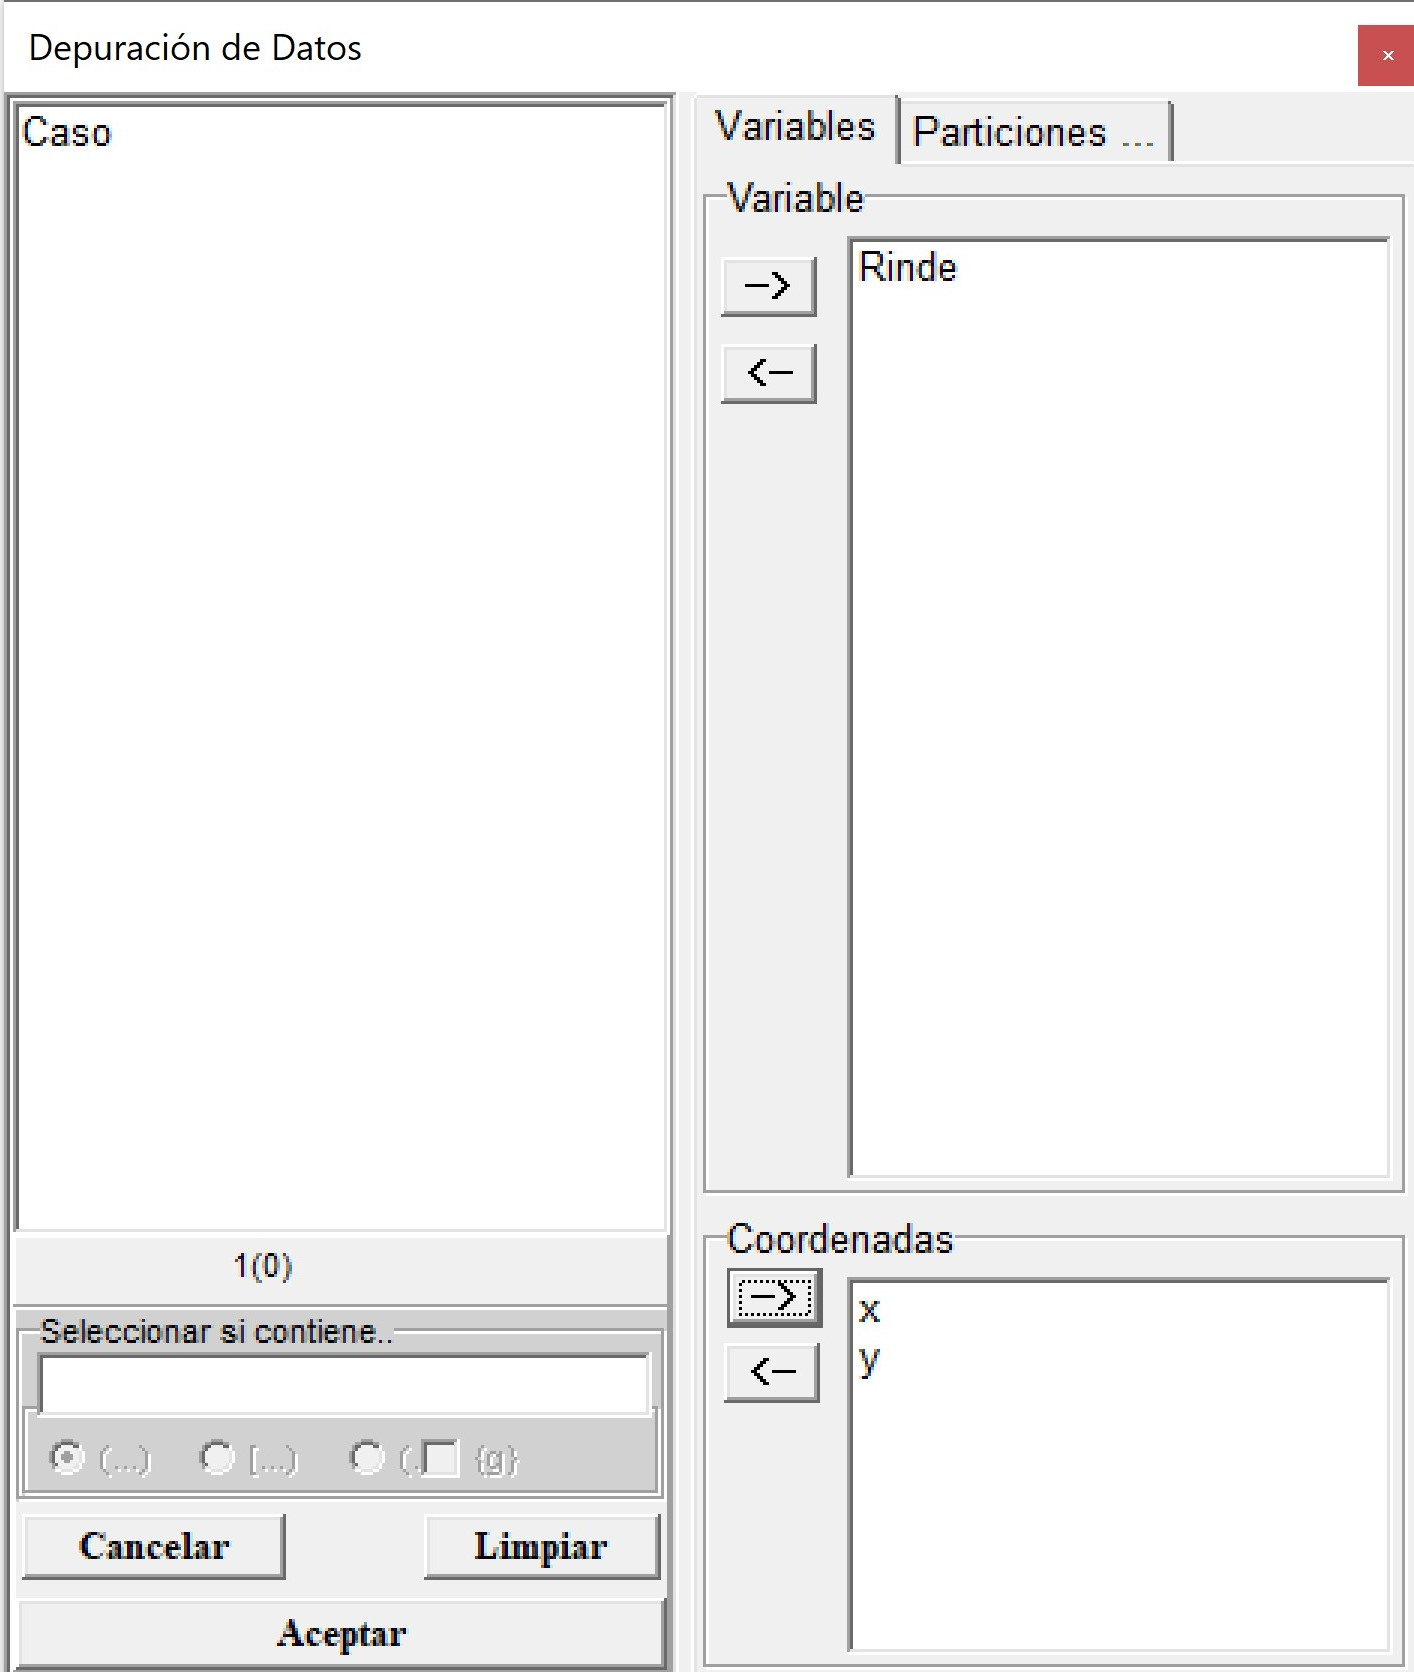
\includegraphics[width=0.7\linewidth]{figuras/Parte2/6} \end{center}

Al accionar el botón \emph{Aceptar}, una nueva ventana permitirá seleccionar si desea visualizar los gráficos \emph{Histograma}, \emph{Box-Plot}, \emph{Red de Vecindarios}, \emph{Visualización espacial} y \emph{Moran Plot}. También existe la opción de tildar que se genere una tabla nueva con los datos depurados, otra tabla con los estadísticos del Índice de Moran y una opción que permite que en la definición de los vecindarios existan algunos puntos que no presenten vecinos. Los valores \emph{inliers} serán identificados a través del Índice de Moran local (\emph{IM local}), \emph{Moran Plot} o ambos (\emph{IM local+Moran Plot}). En la misma ventana hay una opción de seleccionar el valor de desviación estándar (DE) de acuerdo al criterio del usuario. Considerando como valores \emph{outliers} a los que se encuentren fuera del rango estimado como el valor medio ± el valor de DE seleccionado. Por defecto presenta un valor de 3 DE. También el usuario previamente puede limitar los valores de los datos por un valor mínimo y/o máximo. Por defecto este filtro no se aplica.

En este ejemplo se seleccionaron las Opciones \emph{Histograma}, \emph{Box-Plot}, \emph{Visualización espacial}, \emph{Moran plot} y \emph{Tabla datos depurados}. Además, se seleccionó que la eliminación de \emph{inliers} se haga mediante el cálculo del índice de local de Moran y el Moran Plot (\emph{IM local+Moran Plot}). Se utilizó una distancia de 15 para definir los vecindarios y un criterio de 3 DE para la eliminación de \emph{outliers}. Por defecto el código EPSG es 32721 que correspondiente a la base de datos de prueba. En esta rutina el sistema de referencia es importante sólo para realizar la visualización espacial.

\begin{center}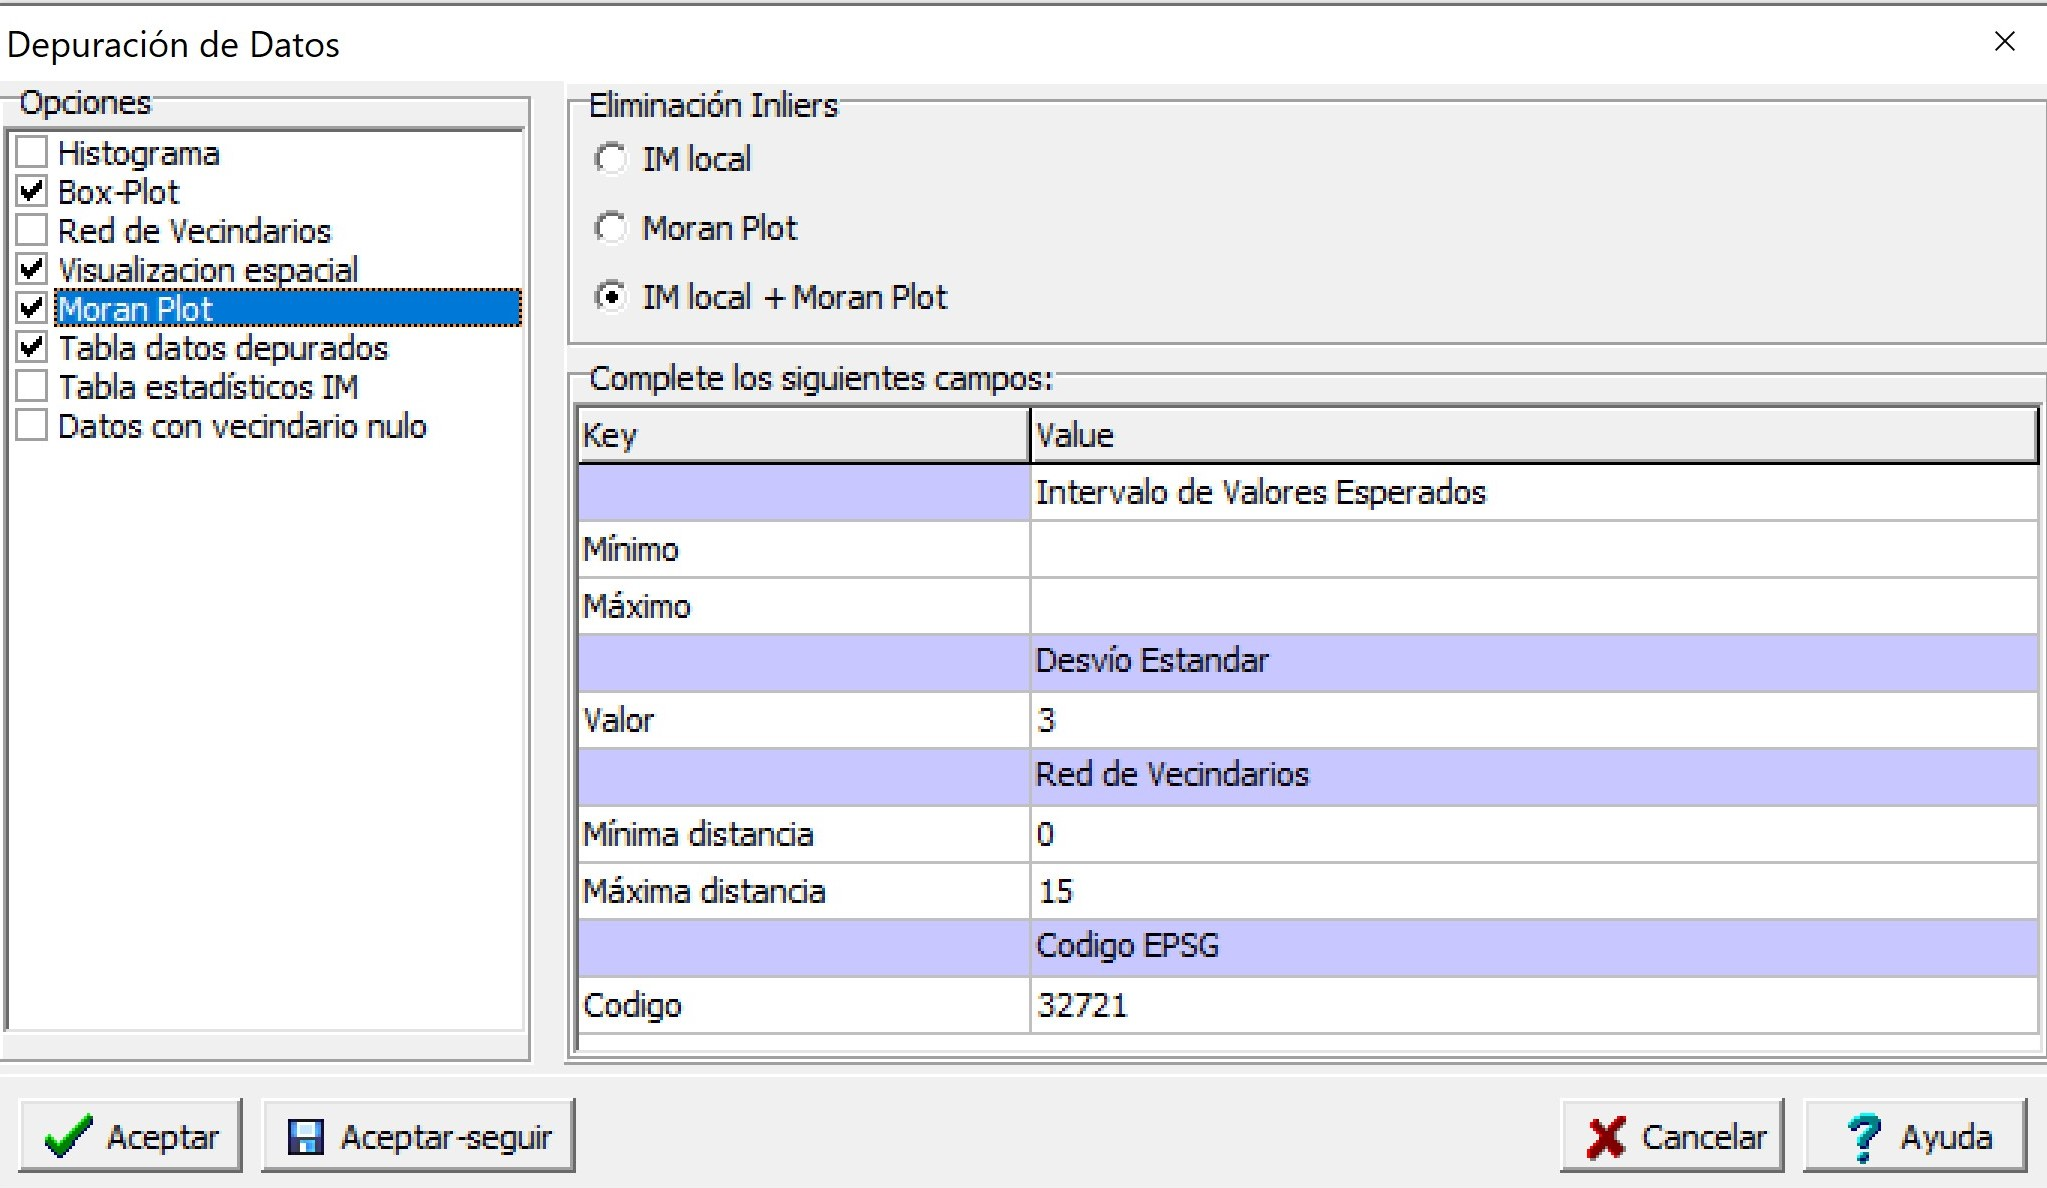
\includegraphics[width=\linewidth]{figuras/Parte2/7} \end{center}

Como resultado se obtendrá el Box-Plot de la variable respuesta (Rinde) previo a la eliminación de los \emph{outliers} e \emph{inliers} (datos sin depurar), y luego de su eliminación (datos depurados). El gráfico de dispersión de Moran (Moran Plot) muestra en el eje horizontal los valores de la variable rendimiento mientras que en el vertical se representa el retardo espacial de la variable. Los puntos negros con forma romboidal son identificados como influyentes y se los considera como \emph{inliers}.

\begin{center}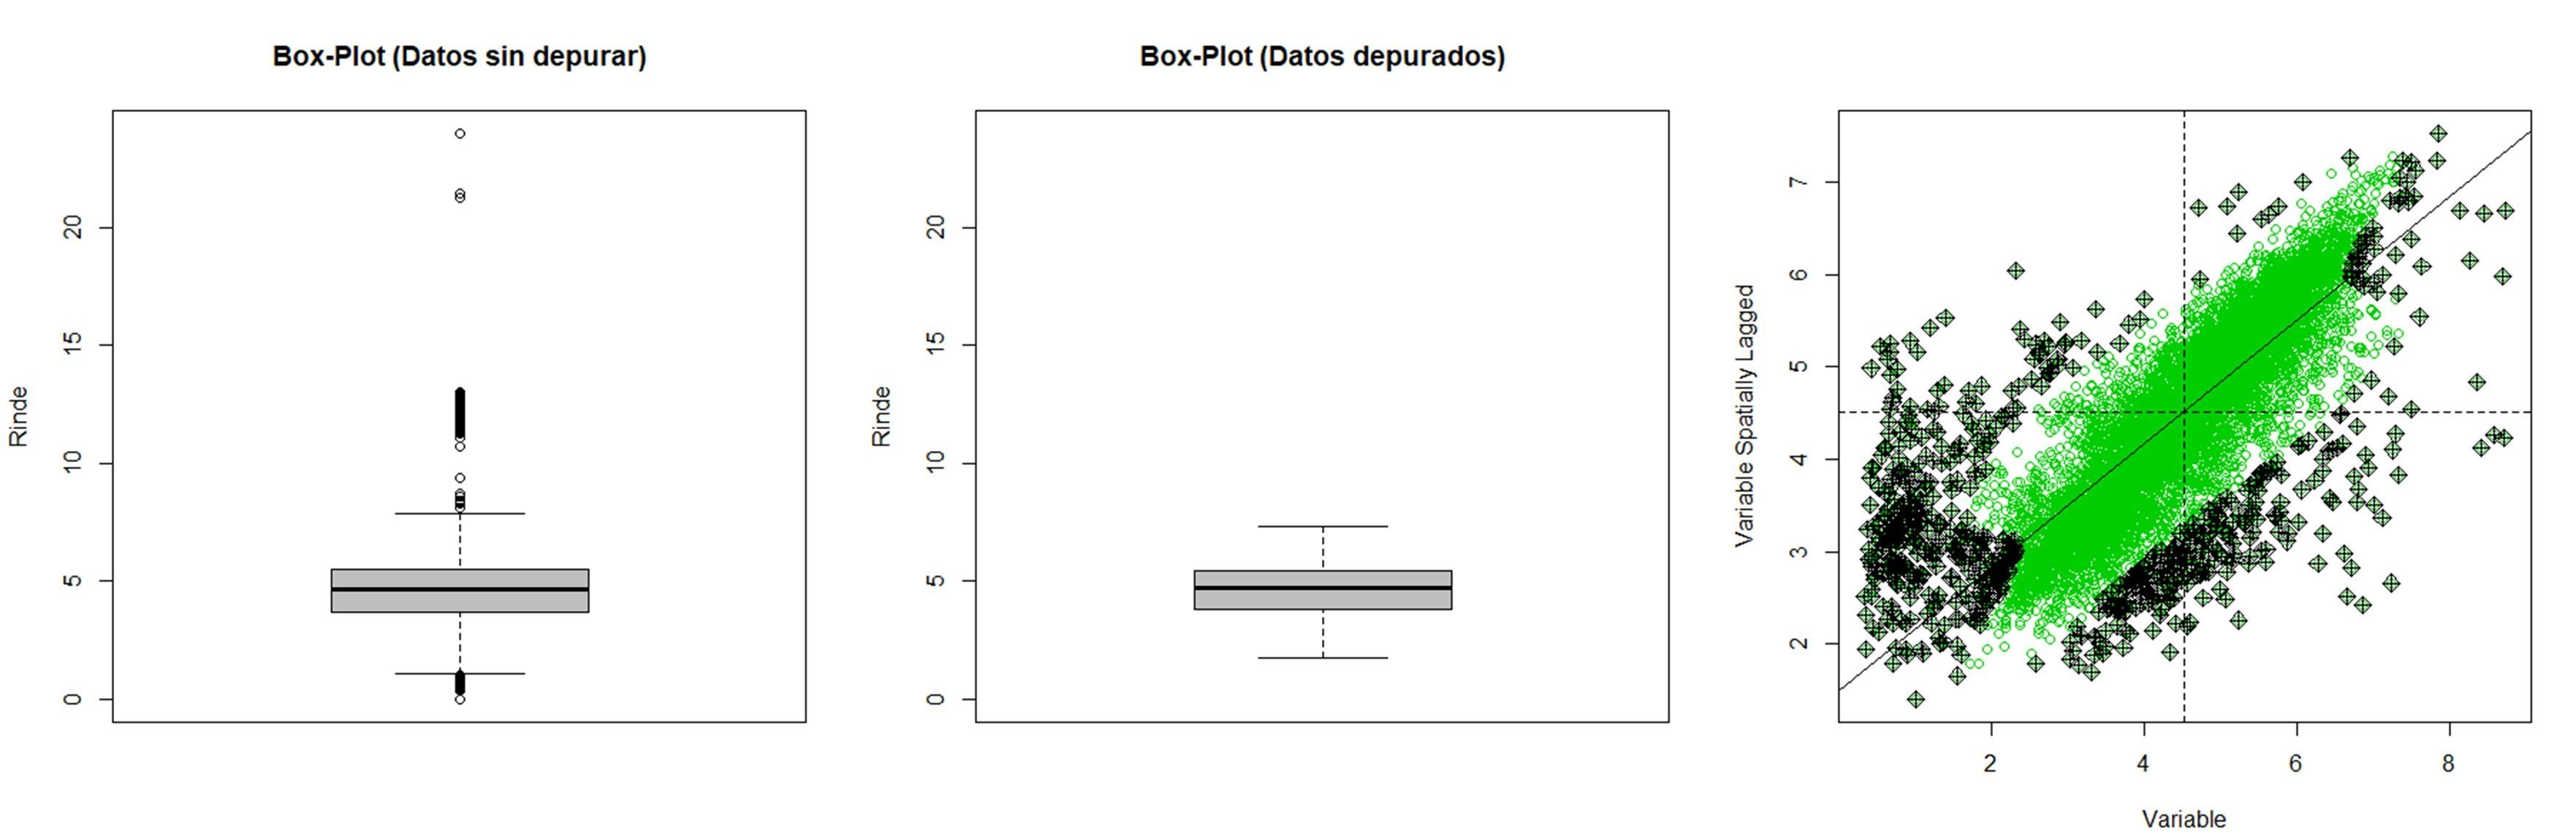
\includegraphics[width=\linewidth]{figuras/Parte2/8} \end{center}

Como resultado de la depuración de datos en la base de datos original se crearán nuevas columnas al final del archivo con la clasificación de \emph{outliers} y/o \emph{inliers} para cada observación. Así, se adicionarán tres columnas denominadas \emph{Outliers}, \emph{Inliers\_ML} e \emph{Inliers\_MP} según el método seleccionado. Estas variables son de tipo categóricas y contendrán la clasificación \emph{Outliers} o \emph{Normal} indicando si es considerado un valor extremo o no. En la columna de \emph{Inliers\_ML}, las categorías serán \emph{Inliers} o \emph{Normal} para indicar que no es un valor atípico respecto a sus vecinos cercanos y de la misma manera se indicarán los valores clasificados por el método de Moran Plot. En este ejemplo, 120 observaciones fueron clasificadas como \emph{outliers}, 43 observaciones como \emph{inliers} y 681 clasificadas como \emph{inliers} según Moran Plot (en los que se encuentran incluidos los 43 casos considerados Inliers por el Índice de Moran Local). El procedimiento primero elimina los \emph{outliers} por lo cual no serán considerados para su identificación como posibles \emph{inliers}.

\begin{center}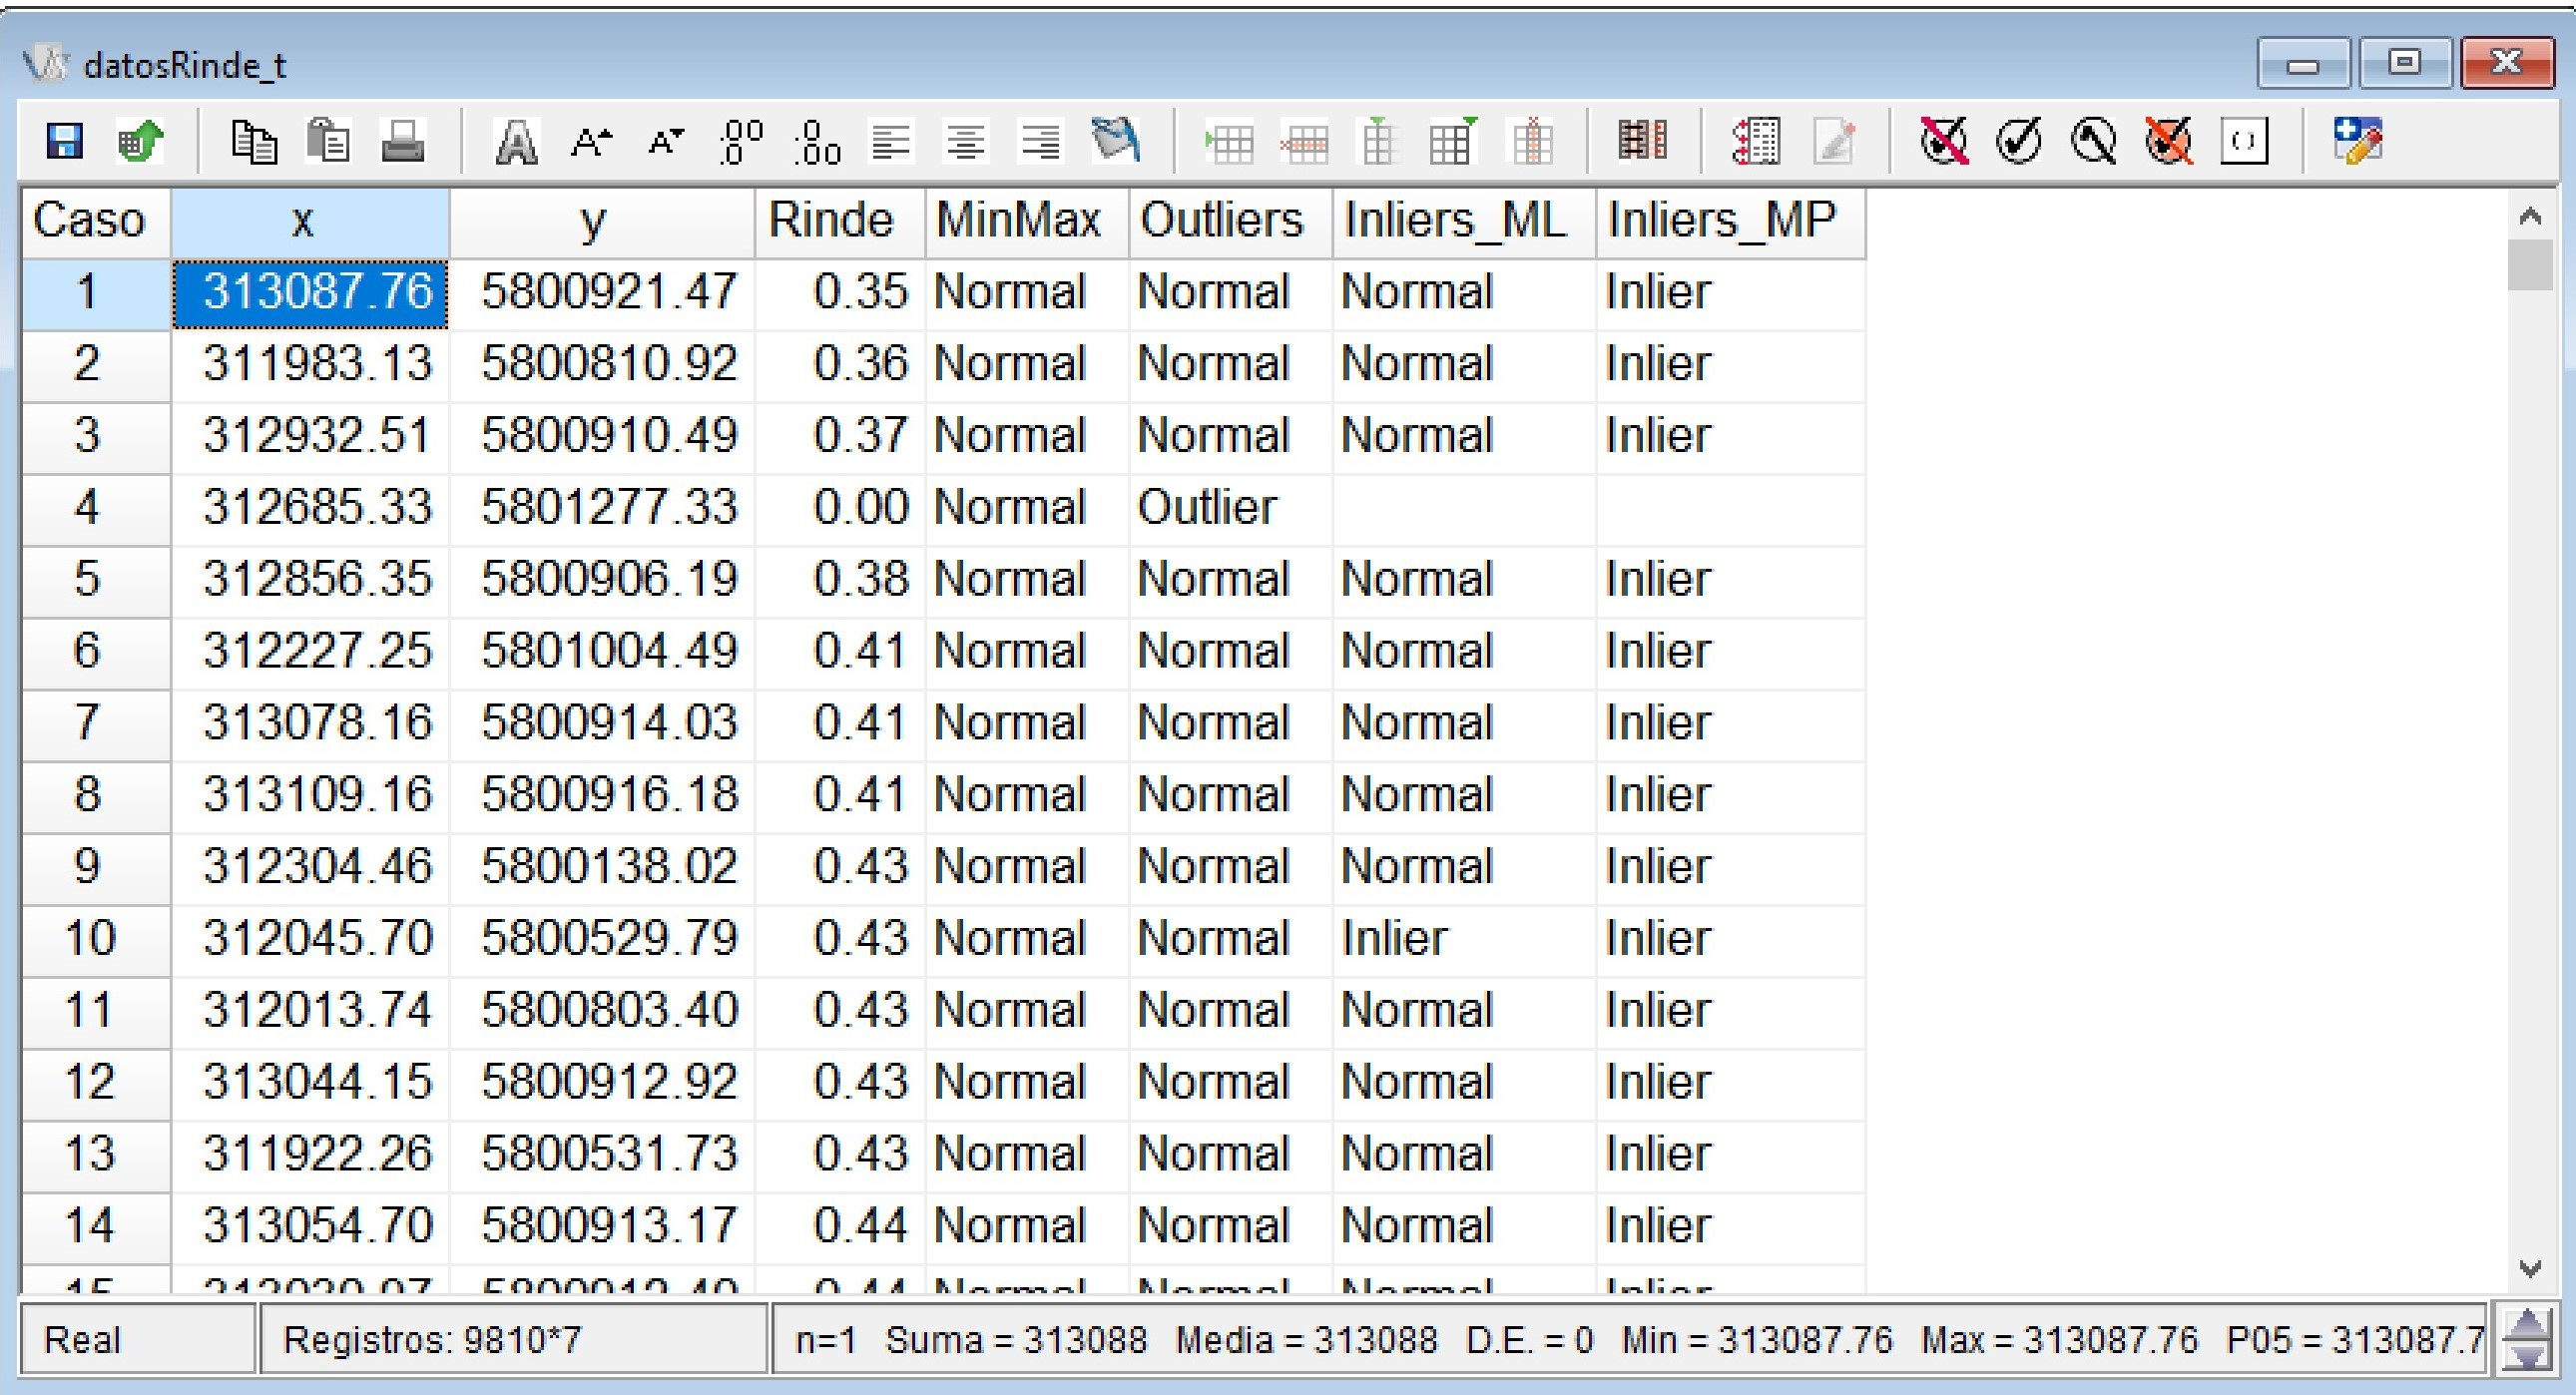
\includegraphics[width=\linewidth]{figuras/Parte2/8b} \end{center}

También se generará una nueva tabla de datos que contendrá las observaciones seleccionadas después de la depuración por \emph{outliers} e \emph{inliers}, que para este ejemplo contiene 9009 registros. Los valores seleccionados se muestran en la tabla denominada \textbf{Datos Depurados.idb2}. En caso que el usuario seleccione \emph{Tabla estadísticos IM} se genera otra tabla \textbf{Estadísticos IM.idb2}, en la cual sus columnas tendrán los valores de índice local observado (li), el valor esperado (E.li), la varianza (Var.li), el estadístico (Z.li) y la significancia estadística a través del valor-p (Pr.z\ldots{}0). La información del Moran Plot de los puntos influyentes de la regresión proviene de diferentes estadísticos de diagnóstico como DFBETAS (dfb.1\_ para la ordenada al origen y dfb.x para la pendiente), DFFITS (dffit), Covratio (cov.r), distancia de Cook (cook.d) y leverage (hat). Para cada uno de los estadísticos aparecerá una nueva columna del archivo con valores TRUE o FALSE según como ha sido clasificada la observación. En la ventana de Resultados de InfoStat se indica las tablas donde se encuentran estos resultados descriptos. Las nuevas tablas generadas son archivos temporarios, es decir, si desea guardar esta información, deberá ir al menú Archivo \(\to\) Guardar tabla y seleccionar el directorio donde desea guardarlo.
La opción de visualización espacial muestra un gráfico el cual se ejecuta como un archivo html en el navegador web. En este se podrá visualizar los datos detectados como \emph{outliers} e \emph{inliers.} Así mismo es posible cargar un mapa base como \emph{esri.WorldImagery}, \emph{OpenStreetMap}, \emph{OpenTopoMap}.

\begin{center}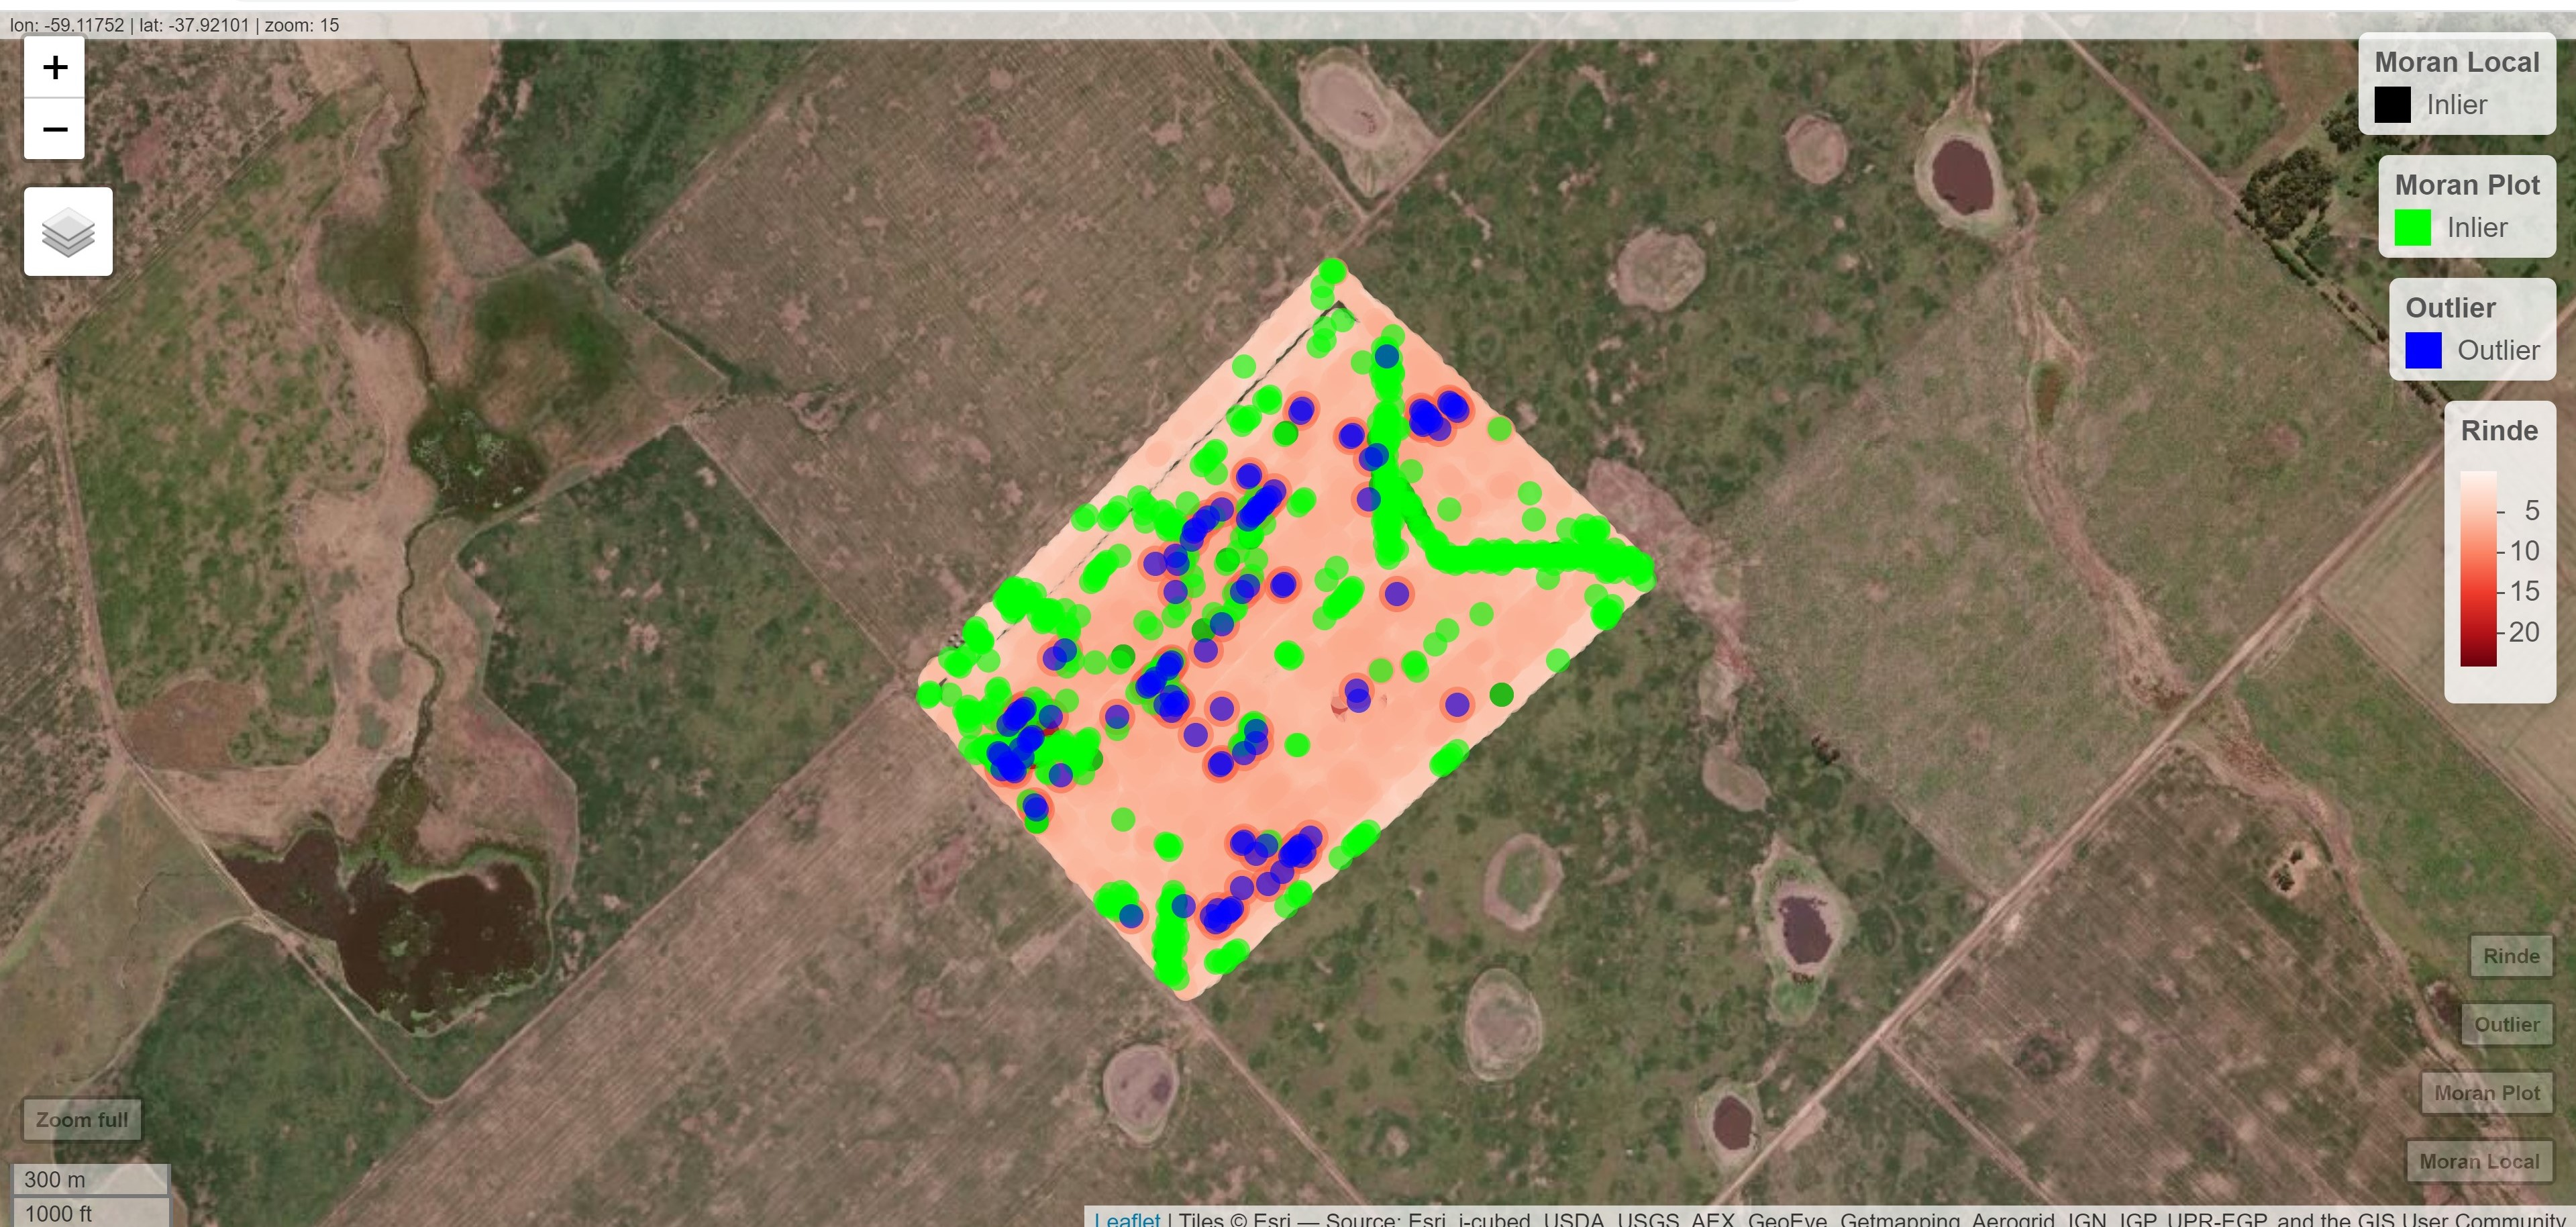
\includegraphics[width=\linewidth]{figuras/Parte2/9} \end{center}

\hypertarget{detecciuxf3n-de-tendencias-espaciales-1}{%
\section{Detección de tendencias espaciales}\label{detecciuxf3n-de-tendencias-espaciales-1}}

Un análisis gráfico para identificar de la presencia de tendencias se puede hacer con un gráfico de dispersión. Para ello ir al menú Gráficos \(\to\) Diagrama de dispersión. En el casiller \emph{Eje Y} colocar la variable \emph{Rinde} y en \emph{Eje X} la coordenada \emph{x}. Al accionar Aceptar se generará el gráfico que muestra que no existe una tendencia entre ambas variables. El mismo procedimiento deber realizarse con la coordenada \emph{y}.

\begin{center}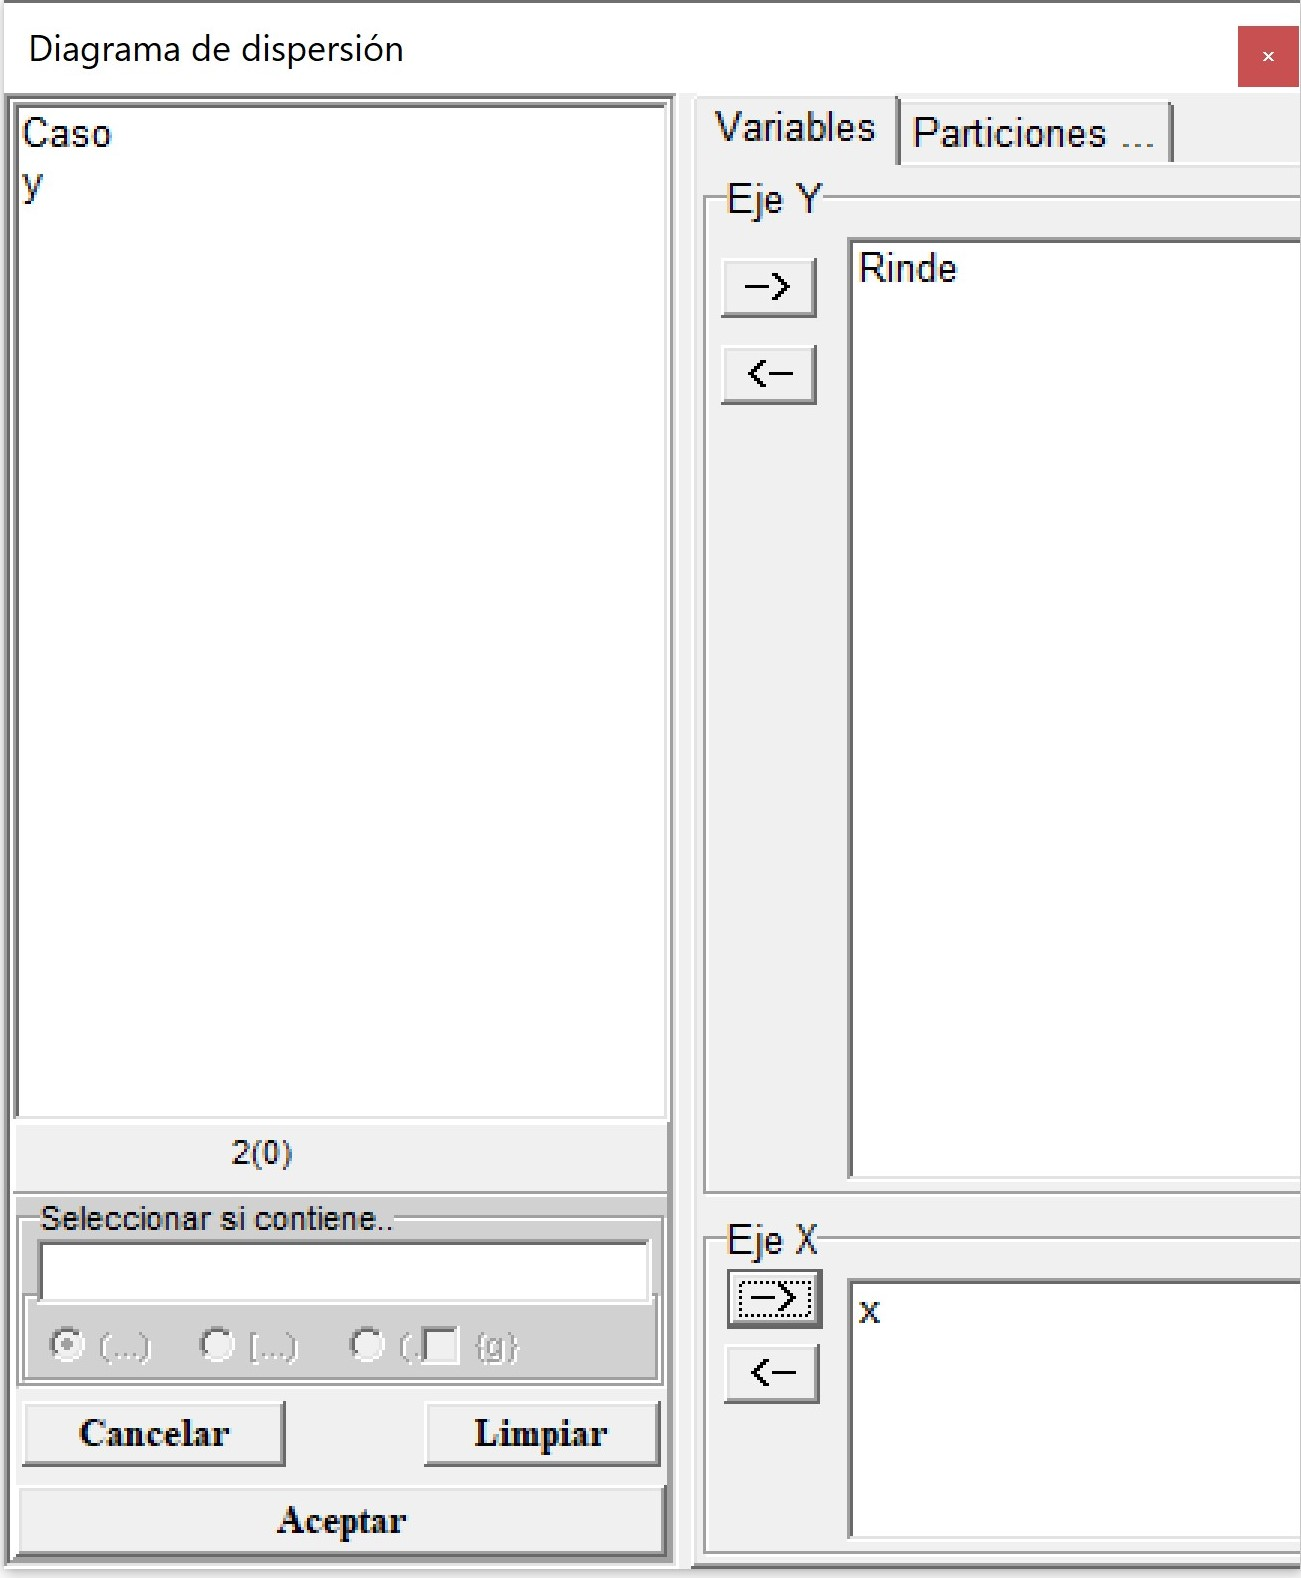
\includegraphics[width=0.7\linewidth]{figuras/Parte2/10} \end{center}

\begin{center}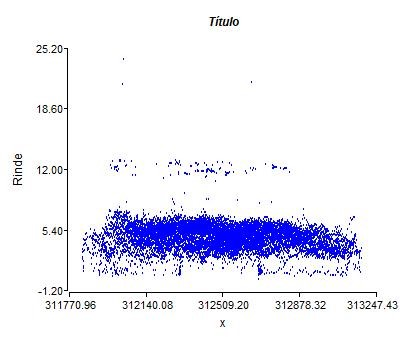
\includegraphics[width=1\linewidth]{figuras/Parte2/11} \end{center}

También es posible ajustar de un modelo de regresión lineal entre la variable Rendimiento y las coordenadas x e y, se puede realizar yendo al menú Estadísticas \(\to\) Regresión Lineal. En el selector de variables se coloca al rendimiento en el casillero de \emph{Variable Dependiente} y las coordenadas x e y en el casillero \emph{Regresoras}.

\hypertarget{cuxe1lculo-del-uxedndice-de-moran-1}{%
\section{Cálculo del índice de Moran}\label{cuxe1lculo-del-uxedndice-de-moran-1}}

Con la base de datos ya depurada en el punto 2.2 se procederá a calcular índices de autocorrelación espacial. El archivo de ejemplo \textbf{datosRinde\_dep.idb2} también se encuentra disponible en el menú Aplicaciones \(\to\) Estadística Espacial \(\to\) Geoestadísticas \(\to\) Semivariograma \(\to\) WLS \(\to\) Datos de prueba. Para cuantificar la magnitud de la estructuración espacial se estiman en este menú el índice de Moran y el índice de Geary. Para ello ir al menú Aplicaciones \(\to\) Estadística Espacial \(\to\) Geoestadísticas \(\to\) Índices de Autocorrelación \(\to\) Run. En el selector de variables colocar \emph{Rinde} en el casillero \emph{Variables} (aquí es posible colocar más de una) y en el casillero \emph{Coordenadas} las columnas x e y.

\begin{center}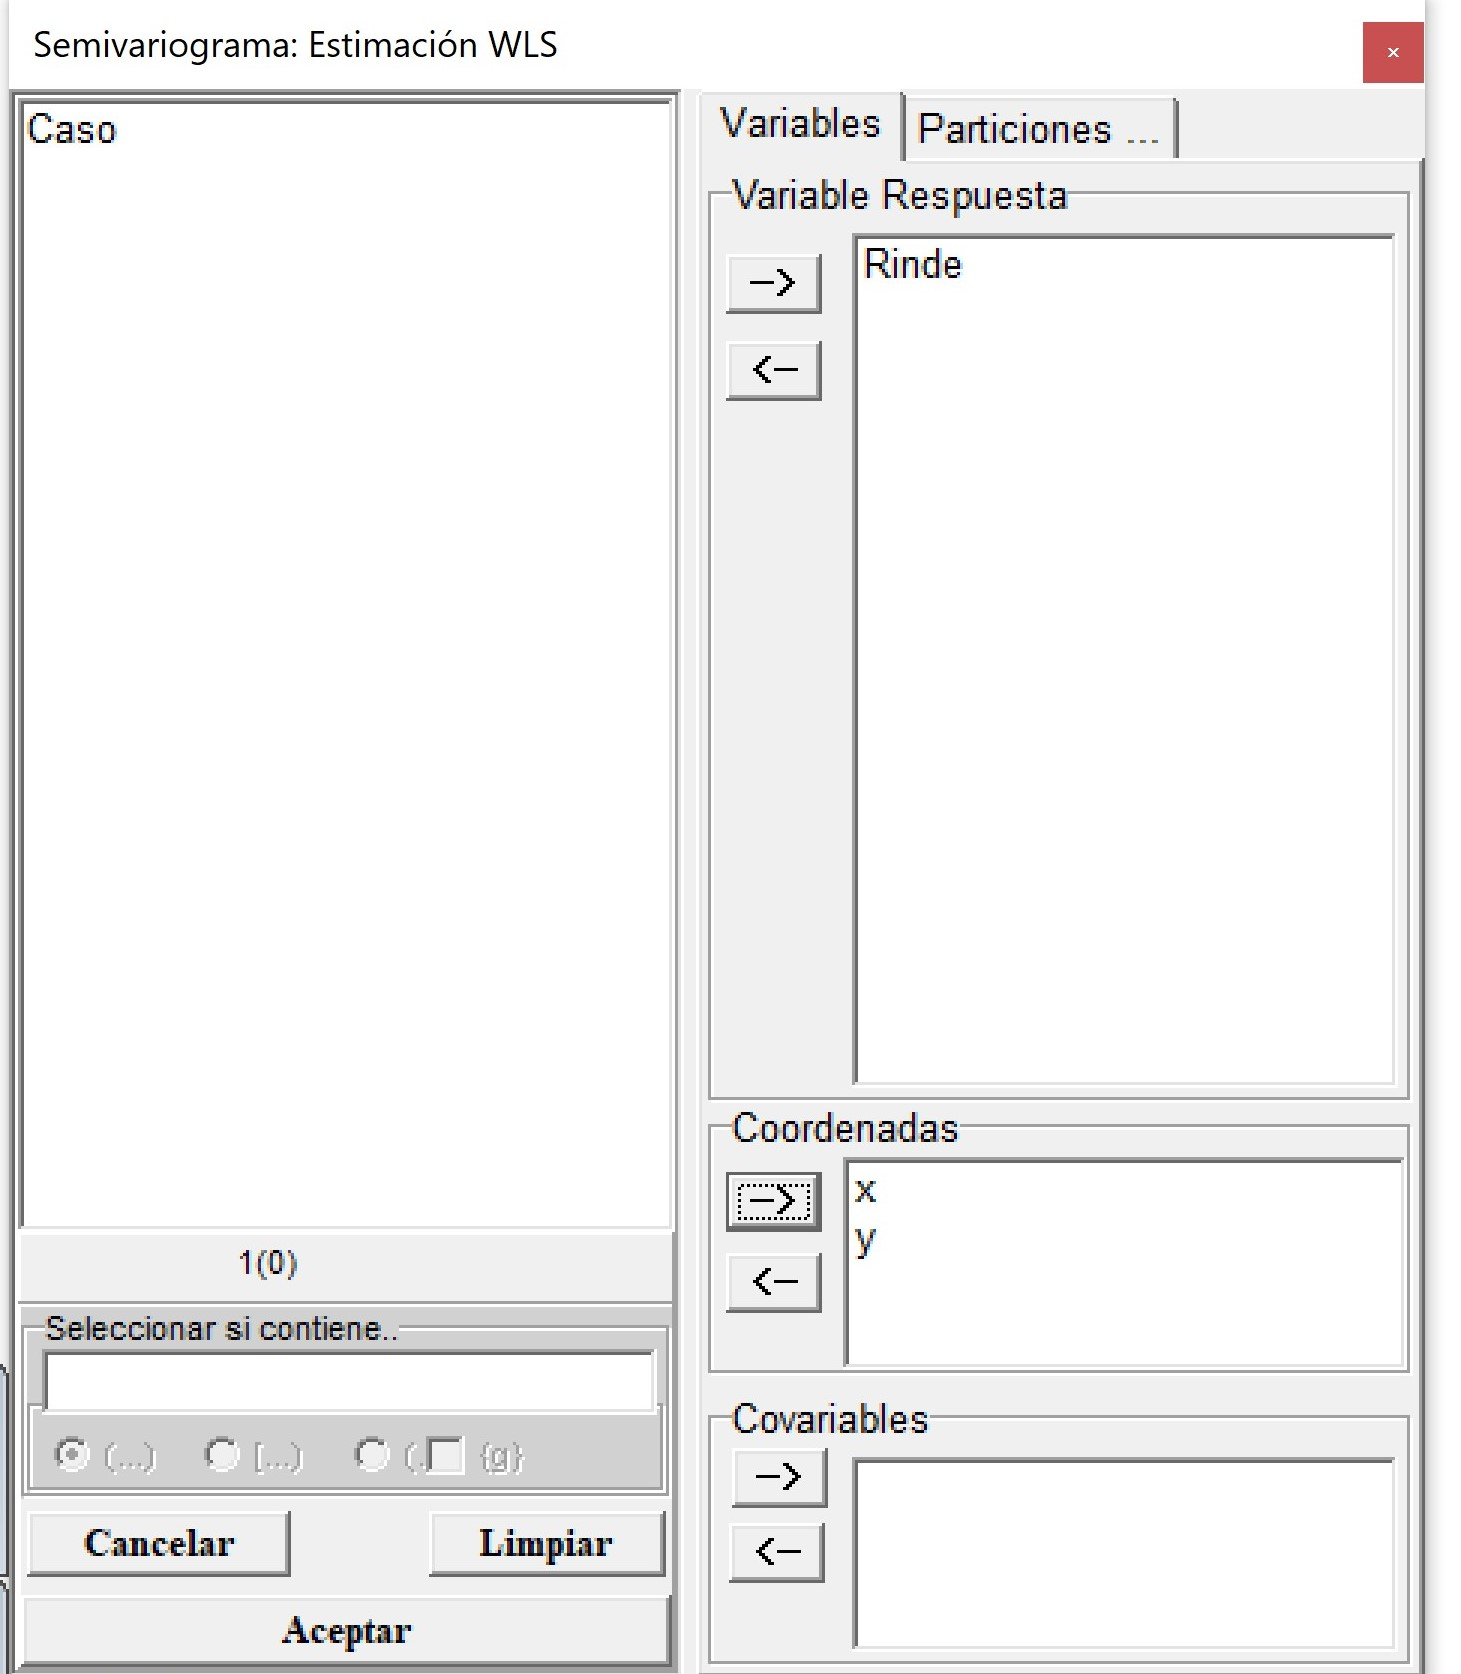
\includegraphics[width=0.7\linewidth]{figuras/Parte2/15} \end{center}

Al accionar \emph{Aceptar} en el siguiente cuadro se puede modificar el número de permutaciones que son utilizadas para evaluar la significancia estadística de los índices a partir de simulación por Monte Carlo. Las ubicaciones son permutadas para obtener la distribución de los índices bajo hipótesis nula de distribución aleatoria. El cálculo también requiere la definición de una matriz de ponderación espacial, para este paso la red de vecindarios es definida usando la distancia Euclídea indicando el rango de distancia dentro de la cual dos observaciones serán consideradas colindantes o vecinas. El rango es estimado a partir de un valor de distancia máximo y uno mínimo. En este ejemplo se utiliza como distancia máxima 15 m. Además, se seleccionó la opción \emph{Datos con vecindario nulo} la cual permite generar la matriz de pesos espaciales sin la restricción de que todos los puntos tengan al menos un dato vecino.

\begin{center}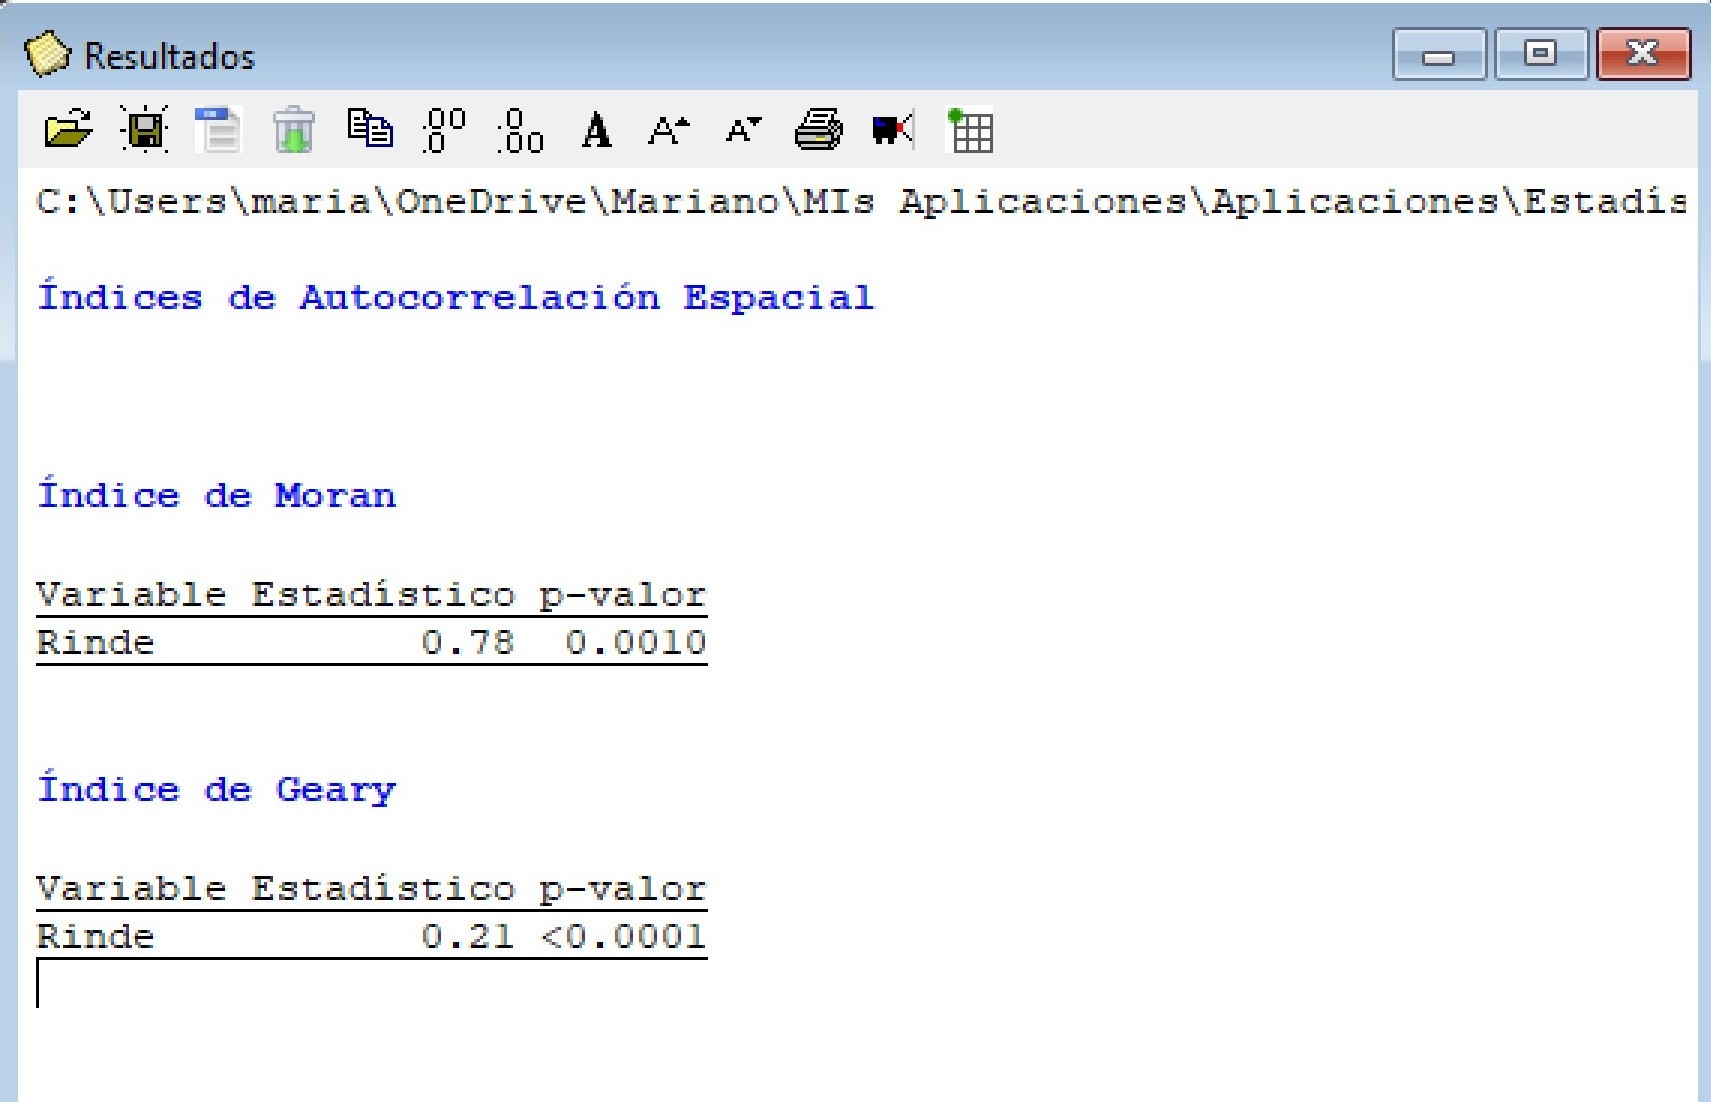
\includegraphics[width=\linewidth]{figuras/Parte2/14} \end{center}

Para este ejemplo, tanto el índice de Moran como el índice de Geary indican una autocorrelación estadísticamente significativa (valor p \textless{}0.05), es decir, no hay una distribución aleatoria de las observaciones en el espacio. La variable Rinde presentó una autocorrelación espacial positiva y alta (valor más cercano a 1 en el caso del índice de Moran y mas cercano a 0 en el de Geary sugieren autocorrelaciones positivas más fuerte).

\hypertarget{anuxe1lisis-basado-en-semivariogramas-1}{%
\section{Análisis basado en semivariogramas}\label{anuxe1lisis-basado-en-semivariogramas-1}}

Para acceder al archivo de ejemplo \textbf{datosRinde\_dep.idb2} se debe ir al menú Aplicaciones \(\to\) Estadística Espacial \(\to\) Geoestadísticas \(\to\) Semivariograma \(\to\) WLS \(\to\) Datos de prueba. Luego se acciona la opción \emph{Run} siguiendo la misma ruta de acceso. Esta opción realizará el ajuste de un semivariograma empírico y teórico usando el método de mínimos cuadrados ponderados (WLS). En el selector de variables se debe colocar la variable \emph{Rinde} en el casillero \emph{Variables} y en el casillero \emph{Coordenadas} las columnas x e y.

\begin{center}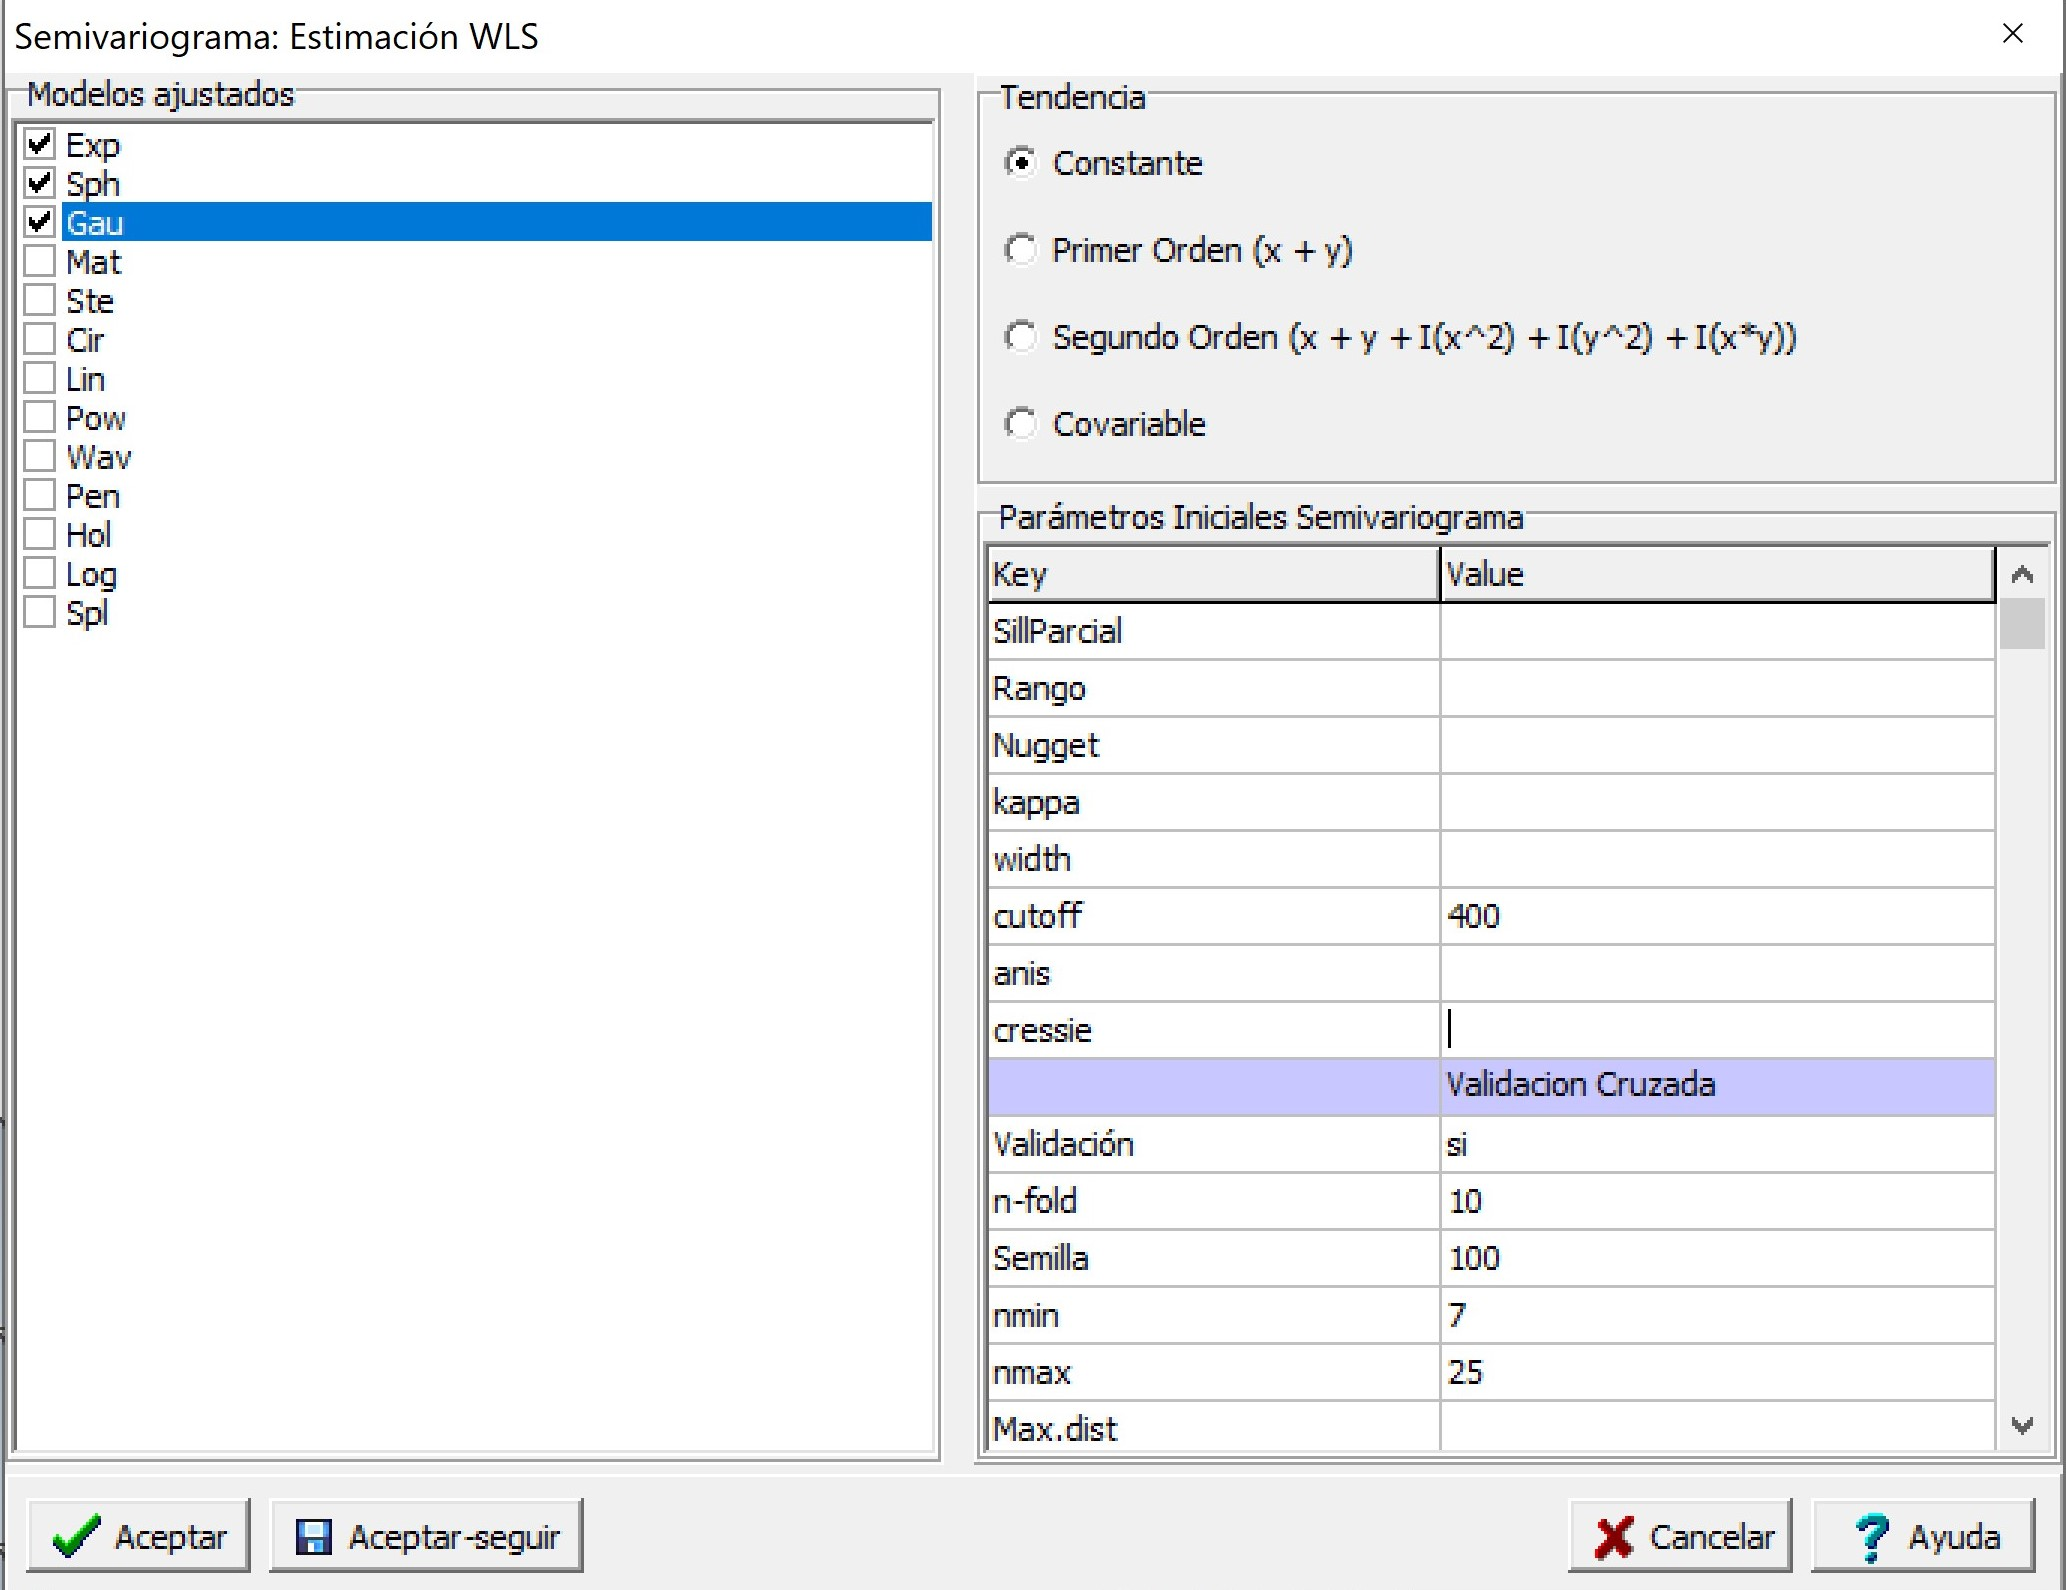
\includegraphics[width=\linewidth]{figuras/Parte2/16} \end{center}

Al accionar el botón \emph{Aceptar}, aparecerá una nueva ventana donde se podrá seleccionar la función de semivariograma: Exp (exponencial), Sph (esférico), Gau (gaussiano), Mat (Matern), Ste (parametrización de Matern Stein), Cir (circular), Lin (lineal), Pow (potencia o power), Wav (ondulado o wave), Pen (pentaesférico), Hol (holístico o hole), Log (logarítmico) y Spl (spline). Como opciones se puede seleccionar ajustar un semivariograma sin tendencia (\emph{Constante}), con tendencia de primer orden, de segundo orden y con covariable. También es posible indicar los valores iniciales para los parámetros del semivariograma a ajustar (SillParcial, Rango y Nugget). En este ejemplo no se colocaron estos por lo cual la función estima valores iniciales razonable para realizar el ajuste. El parámetro \emph{kappa} es opcional para los modelos Matern y Ste (parametrización de Matern Stein). También, puede ser fijado ingresando un valor en la opción \emph{Kappa}. Si en lugar de colocar un valor numérico se coloca un carácter, se ajustará un \emph{kappa} óptimo en un rango entre 0.05 y 5. La opción de parámetro \emph{width} refiere a la amplitud del intervalo de distancia sobre la cual los pares de puntos agrupados para la estimación de la semivarianza. Por ejemplo, si la distancia máxima entre los pares de puntos es de 1000 y se selecciona un valor de \emph{width}=100, se conformarán 10 grupos de una amplitud de 100 m. Para cada uno de esos 10 grupos se estimará la semivarianza. El \emph{cutoff} es la máxima distancia de separación espacial hasta la cual los pares de puntos son tenidos en cuenta para la estimación de la semivarianza. Si la opción queda vacía, es decir no se coloca ningún valor, por defecto estima el \emph{cutoff} como el tercio de la línea diagonal de una caja que contiene los datos. La función por defecto ajusta un semivariograma isotrópico. Para evaluar si el proceso es anisotrópico es posible el ajuste de semivariogramas direccionales. Esto puede hacer desde el menú Aplicaciones \(\to\) Estadística Espacial \(\to\) Geoestadísticas \(\to\) Semivariograma \(\to\) Direccionales. Para incorporar la anisotropía al modelo, en la opción \emph{anis}, se debe colocar la dirección de mayor correlación espacial i.e mayor rango (valor entre 0° y 360°, medidos en el sentido de las agujas del reloj, donde el Norte es 0°.) y el cociente de anisotropía (cociente entre el mayor y el menor rango que se producen en las direcciones evaluadas, valor entre 0 y 1). La dirección y el cociente de anisotropía deben ir separados por coma. El separador de decimales es el punto. Por ejemplo anis=c(90, 0.2) indica que el mayor rango se produce a las 3 en punto (dirección este) con una diferencia de 5 veces en el rango.

La opción \emph{cressie} permite el ajuste del semivariograma teórico mediante el estimador robusto de Cressie- Hawkins. Para seleccionar este estimador debe colocarse un \emph{si} a esta opción, caso contrario utilizara el estimador de los momentos de Matheron. Esta función permite realizar una validación cruzada el tipo k-fold. Para ello se debe colocar \emph{si} en la opción \emph{Validación}. El número de grupos \emph{k} se coloca en la opción \emph{n-fold}. Además, es posible fijar la semilla para que la asignación de cada dato a los grupos \emph{k} no cambie en caso de repetir el proceso. Las opciones \emph{nmin}, \emph{nmax} y \emph{Max.dist} se utilizan para que la función kriging, usada en el proceso de validación, se realice en un contexto local. Por defecto se definen vecindarios con un número mínimo y máximo de vecinos de cada punto a predecir siendo estos de 7 y 25, respectivamente. En caso de omitir estos últimos argumentos la interpolación se realiza en un contexto global.

En este ejemplo, se ajustó un semivariograma experimental a partir de los datos observados y se probaron los modelos exponencial, esférico y gaussiano como modelos de semivariograma teóricos. Sus parámetros iniciales fueron estimados por defecto por la función. El valor del \emph{cutoff} se fijó en 400 m. Además, se realizó una validación cruzada con k=10. Todas las otras opciones se dejaron por defecto.
Al accionar \emph{Aceptar} se generan los gráficos con los tres modelos ajustados. La ventana resultados muestra también la información del semivariograma empírico y cada uno de los modelos teóricos ajustados. Además, se proporcionan los valores de los parámetros estimados, criterios de bondad de ajuste (SCE y AIC), y error de predicción de los modelos ajustados. En este ejemplo siguiendo los criterios de SCE y AIC el modelo de mejor ajuste (valores más bajos de estos indicadores) fue el exponencial. Los valores de los parámetros fueron: Sill Parcial=0,86, rango=64,88, efecto Nugget=0,21. Los resultados de la validación cruzada muestran pequeñas diferencias entre los errores de predicción de los modelos ajustados. Para el caso del modelo exponencial la RMSE relativa a la media de los valores observados (nRMSE) fue del 11,82\% mientras cociente de la desviación cuadrática media (MSDR) fue de 0,60 (más cercano a 1 mejor modelo).

\begin{center}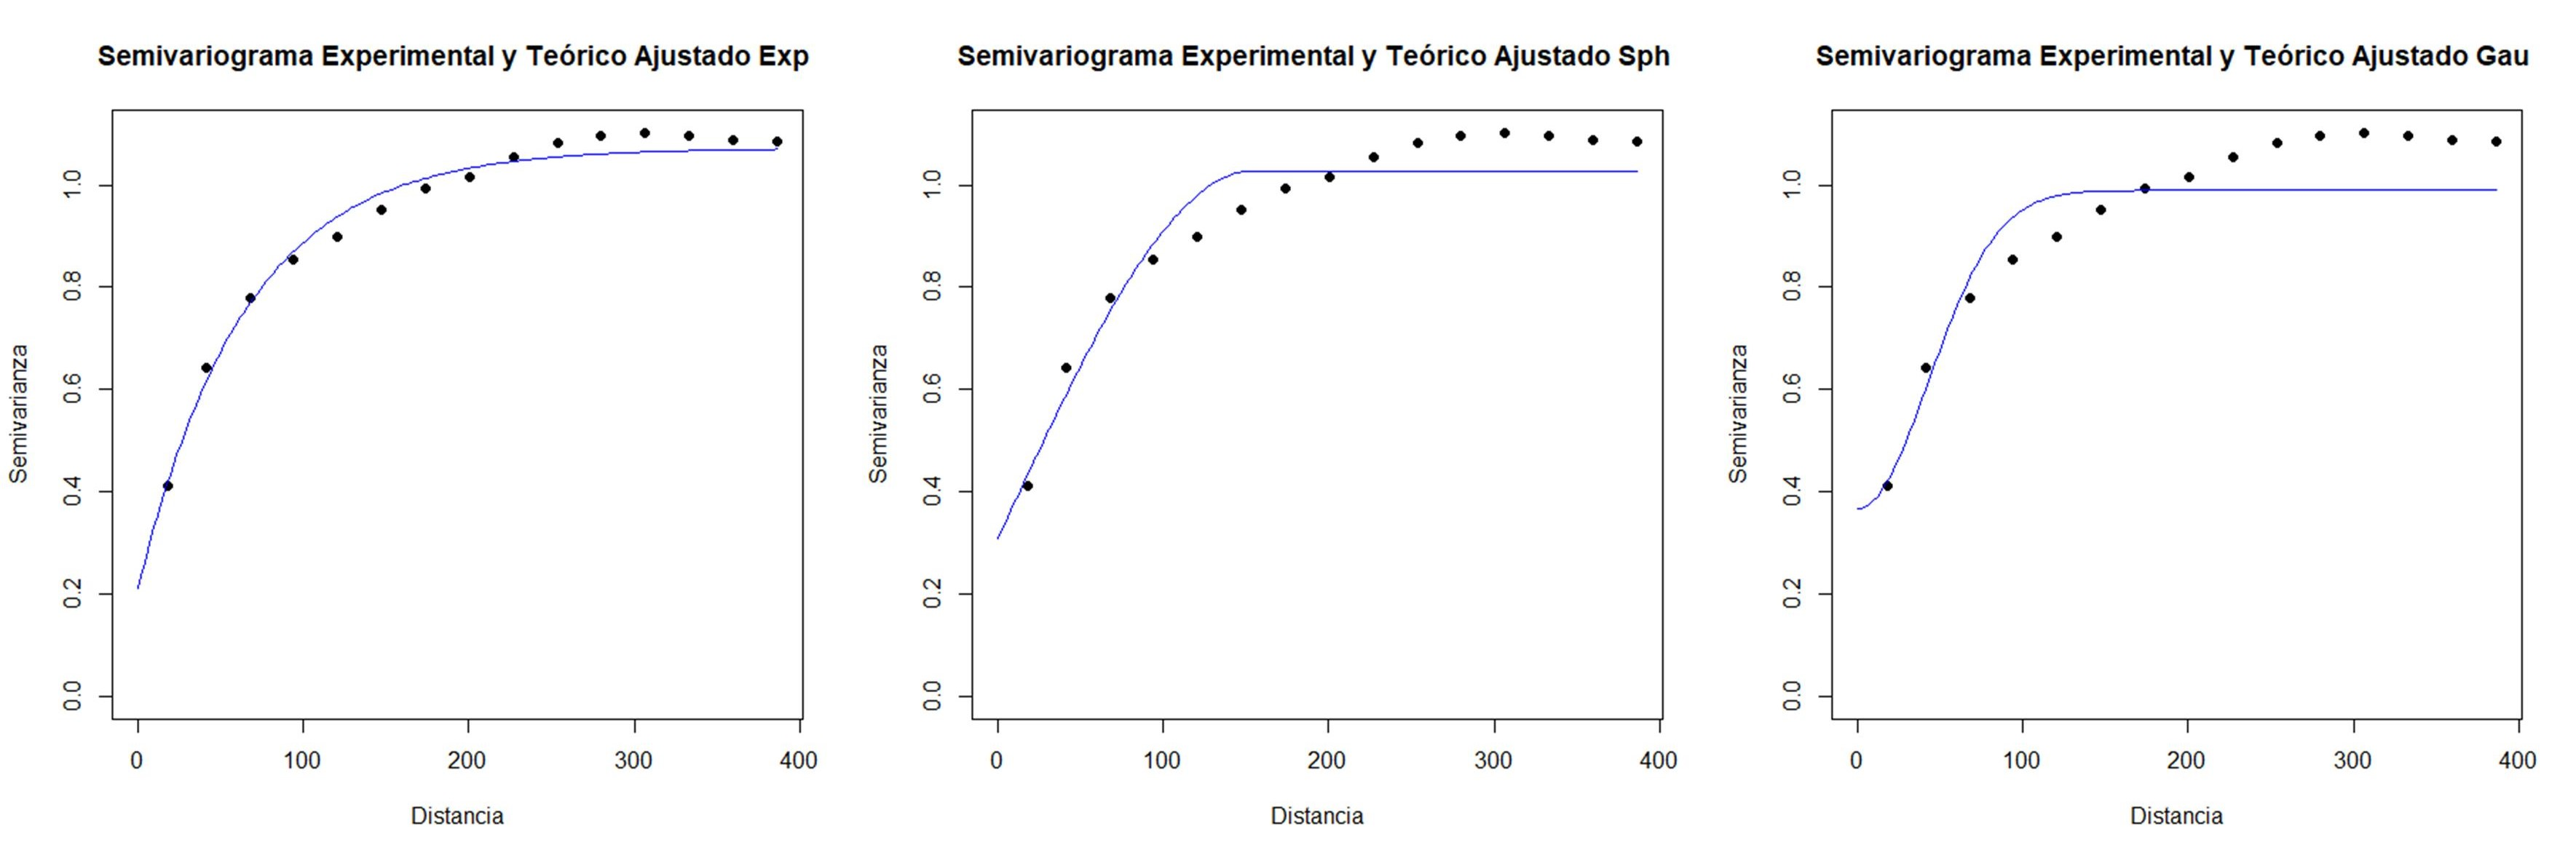
\includegraphics[width=\linewidth]{figuras/Parte2/17} \end{center}

\begin{center}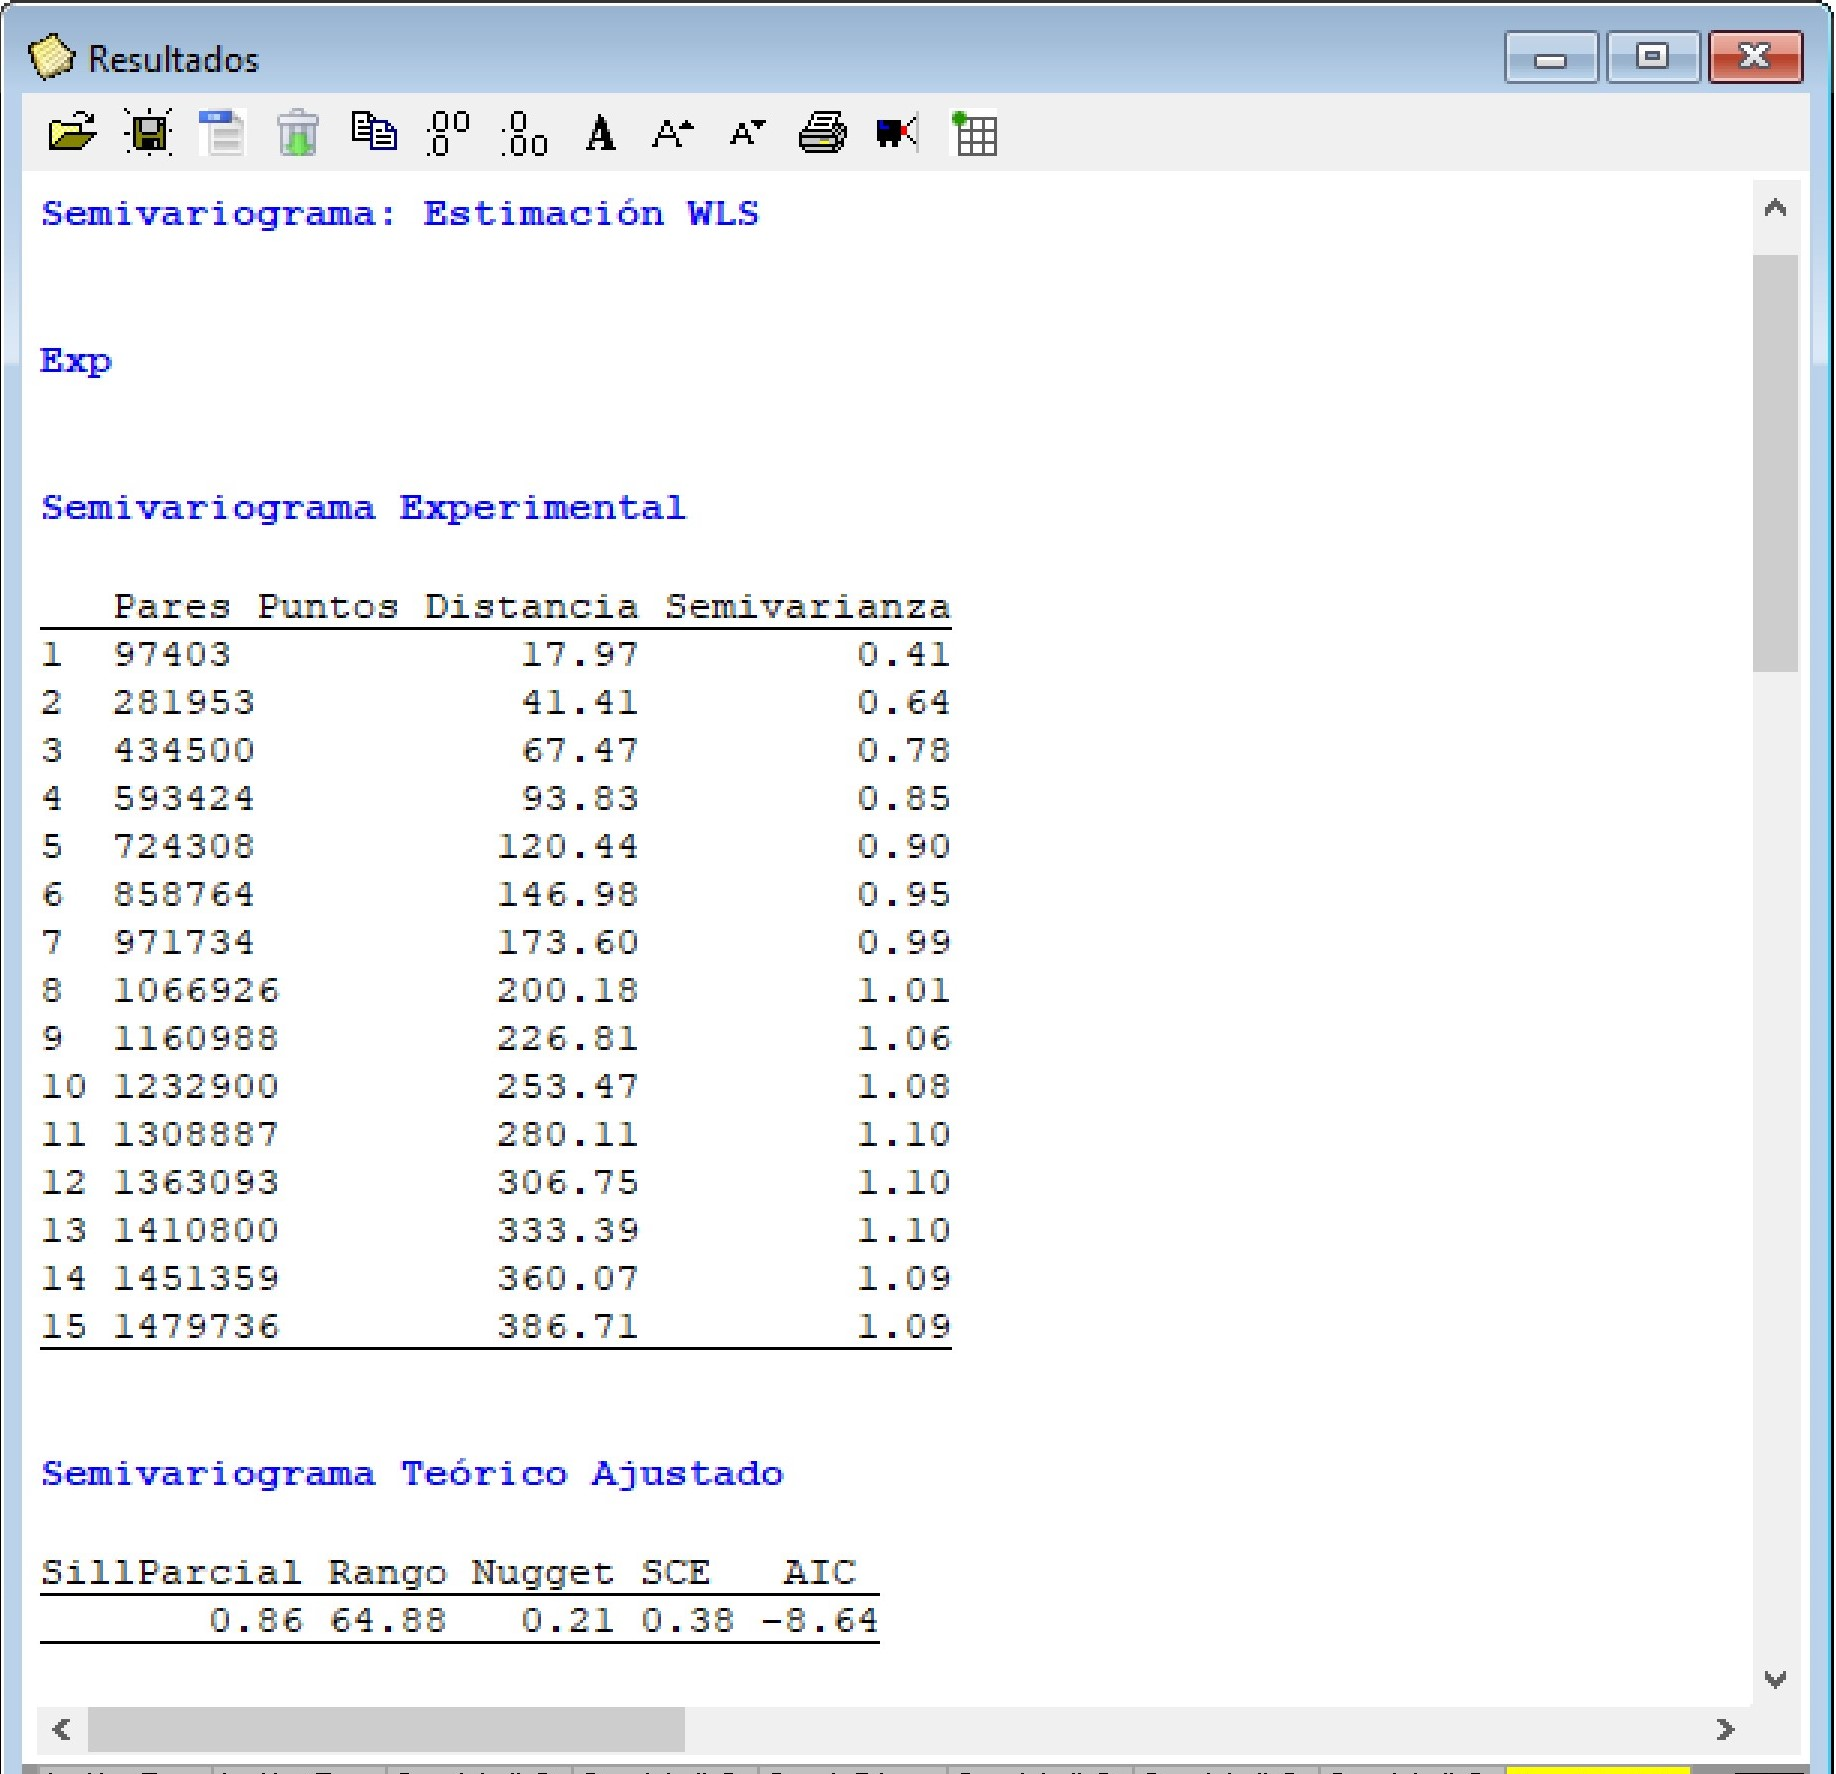
\includegraphics[width=\linewidth]{figuras/Parte2/18} \end{center}

\hypertarget{mapeo-de-variabilidad-espacial}{%
\subsection{Mapeo de variabilidad espacial}\label{mapeo-de-variabilidad-espacial}}

Para realizar la interpolación espacial mediante kriging se utilizará la base de datos \textbf{datosRinde\_limites.idb2} que se encuentra en el menú Aplicaciones \(\to\) Estadística Espacial \(\to\) Geoestadísticas \(\to\) Interpolación \(\to\) Kriging \(\to\) Datos de prueba. El archivo de datos contiene además de las coordenadas (x e y), la variable respuesta (Rinde) y dos nuevas columnas (x1 e y1) que contienen los vértices del polígono donde se desea realizar la interpolación. Estas últimas no son obligatorias para realizar la interpolación. En caso de omitirse la función tomara los puntos más externos de la base de datos y a partir de este formara un polígono que definirán los límites del área a interpolar.

\begin{center}\includegraphics[width=\linewidth]{figuras/Parte2/19} \end{center}

Si se vuelve a la misma ruta de accesos y se acciona \emph{Run} se abrirá el selector de variables donde se colocará la variable \emph{Rinde} en el casillero \emph{Variable Respuesta}, x e y en \emph{Coordenadas} y las columnas x1 e y1 en los casilleros \emph{Coord. Vértices X} y \emph{Coord. Vértices Y}, respectivamente.

\begin{center}\includegraphics[width=0.7\linewidth]{figuras/Parte2/20} \end{center}

Luego de accionar \emph{Aceptar}, se genera una ventana con diferentes opciones para seleccionar el tipo de modelo ajustado (Exp, Sph, Gau, Ste, Cir, Lin, Pow, Wav, Pen, Hol, Log, y Spl), el tipo de kriging, ordinario sin tendencia o universal (incorporando la tendencia en primer o segundo orden) y los valores para realizar la predicción espacial. En este caso se utilizará el modelo seleccionado en el punto anterior. Así, se selecciona el modelo exponencial y se fijan los valores de los parámetros Sill Parcial=0.86, rango=64,88, efecto Nugget=0.21. En este caso la predicción se realiza en un contexto local (opción por defecto). Para ello se fija un número mínimo (\emph{nmin}) y máximo (\emph{nmax}) de puntos que son utilizados para realizar la predicción en cada uno de los sitios de la grilla de predicción. Otra opción para determinar cuáles son los puntos que aportan información para la predicción de un sitio determinado es usando una medida de distancia (\emph{Max.dist}). Puntos que se ubican más allá de la distancia máxima determinada por el usuario respecto a la posición sobre la que se quiere predecir el valor de la respuesta, no serán utilizados para la predicción. En caso de requerir que la predicción se realice utilizando toda la información disponible (kriging global), las opciones \emph{nmin}, \emph{nmax} y \emph{Max.dist} se dejan vacías. La predicción también puede realizarse de manera puntual o en bloque. En este ejemplo donde bloque (Block) es cero, la predicción será local.

Para realizar la predicción se requiere definir los puntos donde se realiza la interpolación en \emph{Opciones de Predicción}. Con \emph{Dim. Grilla Predicción} se fija la dimensión de la grilla de predicción, en este caso, 10 indica que tiene una dimensión de 10×10 m. También puede fijarse el sistema de coordenadas que tendrán los mapas generados usando el código EPSG. Para estos datos el código es 32721 que corresponde al sistema de coordenadas UTM, zona 21, hemisferio sur. Esto es importante para proyectar correctamente los mapas generados. Es posible visualizar estos mapas en el navegador web colocando \emph{si} en la opción \emph{Generar HTML} o exportarlos como geotiff (opción \emph{Generar GeoTIF}). En caso de colocar \emph{si} en esta última opción el software abrirá una ventana para elegir el directorio en el cual se guardará el archivo generado. Los valores de la predicción también pueden ser colocados en forma de tabla mediante la opción \emph{Guardar Predicción}. Finalmente, también es posible cambiar los valores mínimos y máximos de las escalas de valores de los mapas que se generan (Predicción y Varianza de Predicción).

\begin{center}\includegraphics[width=\linewidth]{figuras/Parte2/21} \end{center}

\begin{center}\includegraphics[width=\linewidth]{figuras/Parte2/22} \end{center}

\begin{center}\includegraphics[width=\linewidth]{figuras/Parte2/23} \end{center}

\hypertarget{validaciuxf3n-cruzada-2}{%
\subsection{Validación cruzada}\label{validaciuxf3n-cruzada-2}}

La evaluación de la capacidad predictiva de los modelos ajustados que se realizó en el punto 2.5, también puede realizarse desde el menú Aplicaciones \(\to\) Estadística Espacial \(\to\) Geoestadísticas \(\to\) Interpolación \(\to\) Validación Cruzada. En el selector de variables se coloca la variable \emph{Rinde} en el casillero \emph{Variable Respuesta} y las coordenadas en el cuadro \emph{Coordenadas}.

\begin{center}\includegraphics[width=0.7\linewidth]{figuras/Parte2/24} \end{center}

En la siguiente ventana se coloca la información del modelo a evaluar, en este caso exponencial con parámetros Sill Parcial= 0.86, rango=64.88 y efecto Nugget=0.21. La predicción kriging se realiza en un contexto local (opción por defecto) con \emph{nmin}=7 y \emph{nmax}=25. El número de grupos de la validación cruzada es de k=10. La función permite también calcular el error de predicción para kriging universal (tendencias de primer y segundo orden) y kriging con deriva externa.

\begin{center}\includegraphics[width=\linewidth]{figuras/Parte2/25} \end{center}

Para este ejemplo la RMSE relativa a la media de los valores observados (nRMSE) fue del 10,27\% mientras cociente de la desviación cuadrática media (MSDR) fue de 0.66 (más cercano a 1 mejor modelo).

\begin{center}\includegraphics[width=\linewidth]{figuras/Parte2/26} \end{center}

\hypertarget{caracterizaciuxf3n-de-variabilidad-espacial-con-muxfaltiples-capas-de-datos-2}{%
\section{Caracterización de variabilidad espacial con múltiples capas de datos}\label{caracterizaciuxf3n-de-variabilidad-espacial-con-muxfaltiples-capas-de-datos-2}}

\hypertarget{anuxe1lisis-de-componentes-principales-2}{%
\subsection{Análisis de componentes principales}\label{anuxe1lisis-de-componentes-principales-2}}

La base de datos \textbf{Pred2.idb2} se encuentra disponible en el menú Aplicaciones \(\to\) Estadística Espacial \(\to\) Geoestadísticas \(\to\) Multivariado \(\to\) a. MULTISPATI-PCA \(\to\) Datos de prueba. En el selector de variables se colocan las variables Pe, Elev, CE30, CE90 y Tg en el cuadro \emph{Variables} y las coordenadas x e y en \emph{Coordenadas}.

\begin{center}\includegraphics[width=0.7\linewidth]{figuras/Parte2/27} \end{center}

En la siguiente ventana se presentan las opciones del MULTISPATI-PCA. Aquí se puede seleccionar estandarizar las variables (opción por defecto), generara gráficos (biplot del PCA, gráfico de la red de vecindarios, gráficos del MULTISPATI-PCA y gráfico de los autovalores) y solicitar que la conformación de la matriz de pesos espaciales admita datos con vecindarios nulo. Las otras opciones del análisis implican fijar el número de ejes retenidos por el PCA y por el MULTISPATI-PCA. Para este último caso pueden ser aquellos que presenten una autocorrelación positiva (\emph{MULTISPATI-PCA (+)}) o negativa (\emph{MULTISPATI-PCA (-)}). La parametrización para este ejemplo se muestra en la siguiente figura:

\begin{center}\includegraphics[width=\linewidth]{figuras/Parte2/28} \end{center}

El gráfico obtenido del MULTISPATI-PCA muestra que las variables Elev y Pe son las más importantes en la explicación de la variabilidad espacial a nivel del primer eje (sPC1, eje horizontal). Mientras que la CE30 y Tg presentan mayor importancia en la SPC2. Además, se observa una correlación positiva entre CE30 y CE90, y negativa entre estas dos y la Pe. También la Elev y Tg se correlacionan en forma negativa.

\begin{center}\includegraphics[width=\linewidth]{figuras/Parte2/29} \end{center}

Los resultados muestran que con MULTISPATIPCA se explica una menor proporción de la varianza acumulada en el primer eje, respecto de PCA (1,81 vs.~1,94). Las tres primeras CP del PCA explican 78\% de la variabilidad total mientras que la CS1, CS2 CS3 del MULTISPATI el 73\%. No obstante, los valores del índice de Moran calculados para las tres primeras CPs sugieren que la estimación de autocorrelación aumentó cuando se usó MULTISPATIPCA respecto de la contenida en las CPs del PCA (0,79 vs.~0,68 para el eje 1, 0,43 vs.~0,40 para el eje 2, 0,50 vs.~0,25 para el eje 3).

\begin{center}\includegraphics[width=\linewidth]{figuras/Parte2/30} \end{center}

\hypertarget{anuxe1lisis-de-conglomerados-2}{%
\subsection{Análisis de conglomerados}\label{anuxe1lisis-de-conglomerados-2}}

Para realizar la ilustración se utilizará la base de datos \textbf{Pred.idb2} que se encuentra en el menú Aplicaciones \(\to\) Estadística Espacial \(\to\) Geoestadísticas \(\to\) Multivariado \(\to\) c. Clasificación KMsPC \(\to\) Datos de prueba. El archivo de datos contiene además de las coordenadas (x e y), valores de mediciones de conductividad eléctrica aparente en dos profundidades 0-30 cm (CE30) y 0-90 cm (CE90), elevación (Elev), profundidad de suelo (Pe) y rendimiento de trigo (Tg). Las variables CE30, CE90, Elev Pe y Tg se colocan en el casillero \emph{Variables} y las coordenadas x e y en el cuadro \emph{Coordenadas}.

\begin{center}\includegraphics[width=0.7\linewidth]{figuras/Parte2/31} \end{center}

Al accionar \emph{Aceptar}, aparecerá la ventana para seleccionar opciones del método de análisis. El método KM-sPC primero realiza un análisis de componentes principales espaciales (MULTISPATI-PCA) sobre las variables originales. Luego las variables sintéticas (componentes principales espaciales, sPC) son utilizadas como input del análisis de clúster fuzzy k-means. Por ello, es posible estandarizar las variables para realizar el MULTISPATI-PCA y elegir la opción que permite conformar una matriz de pesos espaciales en presencia de datos con vecindarios nulo. Otras opciones del análisis incluyen la distancia (euclídea o manhattan) utilizada en el método de cluster, el número mínimo y máximo de clúster a generar, el número de iteraciones y el exponente difuso. En este ejemplo se usaron las siguientes opciones: 2 hasta 6 cluster, 100 iteraciones y un valor de 1.3 para el exponente difuso. Para el cálculo de la red de vecindarios, necesario para realizar el MULTISPATI-PCA, la distancia mínima y máxima fue de 0 y 10 m, respectivamente. La opción de varianza explicada (\%) fue del 70, lo que indica que seleccione la cantidad de ejes (componentes principales espaciales) necesarios tal que la varianza total explicada sea mayor o igual a 70\%.

\begin{center}\includegraphics[width=\linewidth]{figuras/Parte2/32} \end{center}

En la ventana resultados se muestra la suma de cuadrados de distancias dentro (SCDD) la cual puede usarse para determinar el número de clúster óptimo. Para esto otros índices son calculados como Xie-Beni, Fukuyama Sugeno, Coeficiente de Partición, Entropía de Partición. Para todos ellos un menor valor del índice implica mejor clasificación. Dado que muchas veces los índices no coinciden se adiciona el cálculo de un índice resumen. Los resultados muestran que, para la mayoría de los índices, incluyendo el resumen, el número de clúster optimo es 2. Cuando se ejecuta el análisis los índices también son graficados en forma conjunta usando una escala normalizada. En este caso también un menor valor del índice en la escala normalizada implica una mejor clasificación.

\begin{center}\includegraphics[width=\linewidth]{figuras/Parte2/33} \end{center}

\begin{center}\includegraphics[width=\linewidth]{figuras/Parte2/34} \end{center}

\hypertarget{predicciuxf3n-con-muxfaltiples-capas-de-datos-2}{%
\section{Predicción con múltiples capas de datos}\label{predicciuxf3n-con-muxfaltiples-capas-de-datos-2}}

Los datos de ilustración \textbf{Pred2.idb2} serán utilizados para cada de las alternativas de predicción disponibles en el menú. El archivo de datos contiene además de las coordenadas (x e y), valores de mediciones de conductividad eléctrica aparente en dos profundidades 0-30 cm (CE30) y 0-90 cm (CE90), elevación (Elev), profundidad de suelo (Pe) y rendimiento de trigo (Tg).

\hypertarget{kriging-con-deriva-externa-1}{%
\subsection{Kriging con deriva externa}\label{kriging-con-deriva-externa-1}}

El acceso al menú es a partir de las opciones: Aplicaciones \(\to\) Estadística Espacial \(\to\) Geoestadísticas \(\to\) Interpolación \(\to\) c. Kriging (KED) \(\to\) Datos de prueba. Para realizar la interpolación se necesita de una grilla de predicción previamente generada en formato de archivo .txt que cuente con la información de las coordenadas (x e y) en las dos primeras columnas y de cada una de las covariables que se usaron en el ajuste del modelo. Se requiere que los nombres de las covariables sean los mismos tanto en la grilla de predicción como en la tabla de observaciones. El archivo \textbf{grilla\_am.txt} contiene esta información.

En primer lugar se procede al ajuste de los semivariograma experimental teórico. Para ello se accede al menú Aplicaciones \(\to\) Estadística Espacial \(\to\) Geoestadísticas \(\to\) b. Semivariograma \(\to\) WLS \(\to\) Run. Las variables CE30, CE90, Elev Pe y Tg se colocan en el casillero \emph{Variables}, las coordenadas x e y en el cuadro \emph{Coordenadas} y Pe, Elev, CE30 y CE90 en el cuadro \emph{Covariables}.

\begin{center}\includegraphics[width=0.7\linewidth]{figuras/Parte2/35} \end{center}

En la siguiente ventana se seleccionan los modelos teóricos a ajustar, en este ejemplo exponencial esférico y gaussiano. En la opción \emph{Tendencia} se selecciona \emph{Covariables}. Las otras opciones de ajuste de los semivariogramas se dejan por defecto. Los resultados muestran que el modelo de mejor ajuste según los valores de SCE y AIC es el exponencial. Los semivariogramas teóricos ajustados se despliegan en forma automática.

\begin{center}\includegraphics[width=\linewidth]{figuras/Parte2/36} \end{center}

\begin{center}\includegraphics[width=\linewidth]{figuras/Parte2/37} \end{center}

\begin{center}\includegraphics[width=\linewidth]{figuras/Parte2/38} \end{center}

Con los valores de los parámetros estimados del semivariograma exponencial se procede a realizar la interpolación espacial. Para ello se accede al menú Aplicaciones \(\to\) Estadística Espacial \(\to\) Geoestadísticas \(\to\) Interpolación \(\to\) c. Kriging (KED) \(\to\) Run. Las variables CE30, CE90, Elev Pe y Tg se colocan en el casillero \emph{Variables}, las coordenadas x e y en el cuadro \emph{Coordenadas} y Pe, Elev, CE30 y CE90 en el cuadro \emph{Covariables}.

\begin{center}\includegraphics[width=0.7\linewidth]{figuras/Parte2/39} \end{center}

En la ventana siguiente se selecciona el modelo de semivariograma exponencial y se colocan los valores de los parámetros estimados en el paso anterior. En este ejemplo se selecciona la opción para mostrar el mapa de predicción en una ventana del navegador web (opción \emph{Generar HTML}). Para ello es importante fijar el sistema de coordenada mediante el código EPSG.

\begin{center}\includegraphics[width=\linewidth]{figuras/Parte2/40} \end{center}

Al \emph{Aceptar} se abrirá una ventana que permite seleccionar la grilla de predicción que en este ejemplo se denomina \textbf{grilla\_am.txt}. Posteriormente se generarán los mapas de predicción y varianza de predicción.

\begin{center}\includegraphics[width=\linewidth]{figuras/Parte2/41} \end{center}

\begin{center}\includegraphics[width=\linewidth]{figuras/Parte2/42} \end{center}

\hypertarget{kriging-desde-modelo-de-regresiuxf3n-1}{%
\subsection{Kriging desde modelo de regresión}\label{kriging-desde-modelo-de-regresiuxf3n-1}}

El acceso al menu es a partir de las opciones: Aplicaciones \(\to\) Estadística Espacial \(\to\) Geoestadísticas \(\to\) Interpolación \(\to\) c. Regression Kriging \(\to\) Datos de prueba. Las variables CE30, CE90, Elev Pe y Tg se colocan en el casillero \emph{Variables} y las coordenadas x e y en el cuadro \emph{Coordenadas}.

\begin{center}\includegraphics[width=0.7\linewidth]{figuras/Parte2/43} \end{center}

En la ventana siguiente se puede seleccionar que el método sólo realice la predicción en base al ajuste de un modelo de regresión lineal o sumando a la predicción los valores interpolados usando kriging ordinario de los residuos del modelo de regresión (\emph{Regresión Lineal + kriging Ordinario}). La función ajusta en forma automática el semivariograma experimental y los modelos teóricos exponencial, esférico y gaussiano. Luego, selecciona el de mejor ajuste según el valor de SCE, y los parámetros de este son usados en la interpolación de los residuos. El método también permite realizar una selección de variables paso a paso (\emph{stepwise}) en ambas direcciones usando el criterio de información de Akaike para evaluar el ajuste de los modelos. Otras opciones incluyen la posibilidad de realizar una validación cruzada k-fold, donde se debe especificar el valor de k y un valor para la semilla. Para ello es necesario colocar \emph{si} en la opción \emph{Evaluar}. También es posible guardar los valores predichos (opción \emph{Predichos}) y obtener la predicción (opción \emph{Predecir}) sobre una nueva base de datos. Para esto se necesita tener un archivo .txt con la información de las coordenadas (x e y) en las dos primeras columnas y de cada una de las covariables que se usaron en el ajuste del modelo. Se requiere que los nombres de las covariables sean los mismos tanto en la grilla como en la tabla de datos. La opción \emph{Importancia} permite elaborar un ranking de la importancia relativa de cada covariable en el modelo ajustado. Esta se calcula en función a la influencia que tiene cada predictor en Error Cuadrático Medio (MSE) del modelo mediante un proceso de permutación de los valores de cada covariable.

\begin{center}\includegraphics[width=0.7\linewidth]{figuras/Parte2/44} \end{center}

Al ejecutar el análisis, dado que se solicitó realizar la predicción, el software mostrará una ventana para seleccionar el archivo .txt que corresponde a la grilla de predicción. En este ejemplo se denomina \textbf{grilla\_am.txt}. Al accionar \emph{Abrir} se procederá con el análisis. En la ventana \emph{Resultados} se menciona que los valores \emph{Predichos} se adicionan a la tabla de datos \textbf{Pred2.idb2}. Además, los valores de la predicción se adicionan a la grilla y se despliegan en una nueva tabla de datos denominada \emph{Predicción}.

\begin{center}\includegraphics[width=\linewidth]{figuras/Parte2/45} \end{center}

\begin{center}\includegraphics[width=\linewidth]{figuras/Parte2/46} \end{center}

Los resultados muestran las medidas para cuantificar el error de predicción, entre estas el error medio absoluto (MAE), la raíz del error cuadrático medio (RMSE), la RMSE relativa a la media de los observados (nRMSE) y un valor de \(R^2\). Los valores muestran un mejor desempeño del kriging regresión vs.~el modelo de regresión lineal múltiple. En el ranking de importancia de las variables explicativas se observa que la elevación fue la variable que contribuyo en mayor medida a explicar la variabilidad del rendimiento de trigo. El semivariograma ajustado sobre los residuos del modelo de regresión lineal muestra la existencia de una estructura de correlación espacial (bajo valor del cociente nugget/sill).

\hypertarget{uxe1rboles-aleatorios-1}{%
\subsection{Árboles aleatorios}\label{uxe1rboles-aleatorios-1}}

Para realizar el análisis las variables CE30, CE90, Elev Pe y Tg se colocan en el casillero \emph{Variables} y las coordenadas x e y en el cuadro \emph{Coordenadas}.

\begin{center}\includegraphics[width=0.7\linewidth]{figuras/Parte2/48} \end{center}

En la ventana siguiente se puede seleccionar que el método sólo realice la predicción en base al algoritmo \emph{Random Forest} o sumando a la predicción de este los valores interpolados usando kriging ordinario de los residuos del Random Forest (\emph{Random Forest + kriging Ordinario}). Luego, selecciona el de mejor ajuste según el valor de SCE, y los parámetros de este son usados en la interpolación de los residuos. La función ajusta en forma automática el semivariograma experimental y los modelos teóricos exponencial, esférico y gaussiano. El método también permite fijar un valor del hiperparámetro \emph{mtry} del random forest o también realizar una selección del \emph{mtry} optimo mediante un proceso de validación cruzada del tipo k-fold. Para la validación se puede especificar el valor de k y un valor de semilla. En caso de no fijar el valor de \emph{mtry} utiliza el recomendado de \(p/3\) para modelos de regresión o \(\sqrt{p}\) para modelos de clasificación. Si se quiere probar más de un valor se puede especificar un vector de valores que inician con el valor colocado en la opción \emph{Desde} hasta el valor especificado en \emph{Hasta} con un salto dado por la opción \emph{Paso}. La opción \emph{Evaluar} permite realizar una validación cruzada de la misma forma que la especificada inicialmente. Para ello es necesario colocar \emph{si} en dicha opción.

También, es posible guardar los valores predichos (opción \emph{Predichos}) y obtener la predicción (opción \emph{Predecir}) sobre una nueva base de datos. Para tal fin se necesita tener un archivo .txt de la grilla de predicción con la información de las coordenadas (x e y) en las dos primeras columnas y de cada una de las covariables que se usaron en el ajuste del modelo. Se requiere que los nombres de las covariables sean los mismos tanto en la grilla como en la tabla de datos. La opción \emph{Importancia} devuelve un ranking de la importancia relativa de cada covariable en el modelo ajustado, que se calcula en función a la influencia que tiene cada predictor en Error Cuadrático Medio (MSE) del modelo mediante un proceso de permutación de los valores de cada covariable. La opción \emph{Relaciones Parciales} generar un gráfico que muestra el efecto marginal de cada una de las covariables sobre la variable respuesta. Para obtener este gráfico debe colocarse \emph{si}. Esto genera un panel con los gráficos de cada una de las covaraiables del modelo. Si en lugar de \emph{si} se coloca el carácter \emph{m} el método genera un gráfico independiente para cada una de las regresoras. También, es posible editar los valores mínimos y máximos de la variable respuesta (eje y) en todos los gráficos mediante las opciones \emph{ymin} e \emph{ymax}.

\begin{center}\includegraphics[width=0.7\linewidth]{figuras/Parte2/49} \end{center}

Al ejecutar el análisis, dado que se solicitó realizar la predicción, el software mostrará una ventana para seleccionar el archivo .txt que corresponde a la grilla de predicción. En este ejemplo se denomina \textbf{grilla\_am.txt}. Al accionar \emph{Abrir} se procederá con el análisis. En la ventana \emph{Resultados} se menciona que los valores \emph{Predichos} se adicionan a la tabla de datos \textbf{Pred2.idb2}. Además, los valores de la predicción se adicionan a la grilla y se despliegan en una nueva tabla de datos denominada \emph{Predicción}.

\begin{center}\includegraphics[width=\linewidth]{figuras/Parte2/50} \end{center}

\begin{center}\includegraphics[width=\linewidth]{figuras/Parte2/51} \end{center}

Los resultados muestran las medidas para cuantificar el error de predicción, entre estas el error medio absoluto (MAE), la raíz del error cuadrático medio (RMSE), la RMSE relativa a la media de los observados (nRMSE) y un valor de \(R^2\). Los valores muestran un mejor desempeño del kriging regresión vs.~el modelo de regresión lineal múltiple. En el ranking de importancia de las variables explicativas se observa que la elevación fue la mayor contribución en la determinación del rendimiento de trigo. El gráfico de las relaciones parciales muestra que cuando aumenta la elevación disminuye el rendimiento de trigo. Con la variable Pe la correlación es negativa mientras que con la conductividad eléctrica presenta una relación no lineal. El semivariograma ajustado sobre los residuos del modelo de regresión lineal muestran la existencia de una estructura de correlación espacial (bajo valor del cociente nugget/sill).

\begin{center}\includegraphics[width=\linewidth]{figuras/Parte2/52} \end{center}

\begin{center}\includegraphics[width=\linewidth]{figuras/Parte2/53} \end{center}

\cleardoublepage

\hypertarget{part-anuxe1lisis-de-datos-a-escala-regional}{%
\part{Análisis de datos a escala regional}\label{part-anuxe1lisis-de-datos-a-escala-regional}}

\setcounter{chapter}{0}

\hypertarget{bases-de-datos-regionales}{%
\chapter{Bases de datos regionales}\label{bases-de-datos-regionales}}

Muchos procesos aleatorios varían de manera continua en el espacio a escala regional. Entonces, es de interés predecir el comportamiento de una variable en referencia a su ubicación geográfica. En algunas situaciones además de la distribución en el espacio otras capas de información (covariables de sitio) pueden ser usadas para mejorar la predicción en un sitio específico. En esta parte se ilustran el manejo de datos espaciales para la predicción a escala regional de una variable a partir de múltiples capas de información y la construcción de un modelo de predicción espacial vía estrategias metodológicas alternativas: regresión múltiple vía REML, regresión múltiple vía INLA y regresión no lineal vía modelo basado en árbol.

Como ejemplo se utiliza la base de datos \textbf{suelos\_cba.txt}. Esta es una parte del SIG de los suelos del horizonte superficial de la provincia Córdoba (Hang et~al., \protect\hyperlink{ref-Hang2015}{2015}), que contiene 350 sitios caracterizados por múltiples variables edáficas que describen los primeros 15 cm de profundidad. Las variables presentes en \textbf{suelos\_cba.txt} son: COS (Carbono Orgánico de Suelo, g/kg) arcilla (\%), pH, elevación (m.s.n.m.), twi (Índice Topográfico de Humedad). El objetivo del análisis es ajustar modelos que expliquen la variabilidad espacial de COS en función de las restantes variables en la base de datos.

Para seguir la ilustración, cargar los paquetes específicos de R que albergan las funciones que se utilizarán tanto para el manejo como para la modelación.

\begin{Shaded}
\begin{Highlighting}[]
\KeywordTok{library}\NormalTok{(sf)}
\KeywordTok{library}\NormalTok{(raster)}
\KeywordTok{library}\NormalTok{(tmap)}
\KeywordTok{library}\NormalTok{(nlme)}
\KeywordTok{library}\NormalTok{(INLA)}
\KeywordTok{library}\NormalTok{(caret)}
\KeywordTok{library}\NormalTok{(gstat)}
\end{Highlighting}
\end{Shaded}

\hypertarget{manejo-de-datos-espaciales-1}{%
\section{Manejo de datos espaciales}\label{manejo-de-datos-espaciales-1}}

Mediante la función \texttt{read.table()} se lee un archivo de texto que se guarda como un objeto denominado \texttt{suelos}, en el cual las columnas están separadas por tabuladores y la primera fila contiene los nombres de columnas. Mediante la función \texttt{head()} se visualizan las primeras filas del objeto \texttt{suelos} donde se observa que la primera columna corresponde a una identificación, las siguientes dos son las coordenadas X e Y las cuales corresponden al sistema de proyección UTM faja 20. Las columnas siguientes contienen las variables en estudio.

\begin{Shaded}
\begin{Highlighting}[]
\NormalTok{suelos <-}\StringTok{ }\KeywordTok{read.table}\NormalTok{(}\StringTok{"datos/suelos_cba.txt"}\NormalTok{, }
                     \DataTypeTok{sep =} \StringTok{"}\CharTok{\textbackslash{}t}\StringTok{"}\NormalTok{, }\DataTypeTok{header =} \OtherTok{TRUE}\NormalTok{)}
\KeywordTok{head}\NormalTok{(suelos)}
\CommentTok{#> ID_2 X Y elevacion twi arcilla pH COS}
\CommentTok{#> 1 2 603164 6576899 100 135 30,8 6,6 26,0}
\CommentTok{#> 2 3 596537 6390518 87 133 24,0 7,4 17,3}
\CommentTok{#> [ reached 'max'}
    \OperatorTok{/}\StringTok{ }\KeywordTok{getOption}\NormalTok{(}\StringTok{"max.print"}\NormalTok{) }\OperatorTok{--}
\NormalTok{omitted }\DecValTok{4}\NormalTok{ rows ]}
\end{Highlighting}
\end{Shaded}

Para transformar este objeto en uno de clase espacial, se utilizará la función \texttt{st\_as\_sf()}, especificando que las coordenadas X e Y, se encuentra en las columnas ``X'' e ``Y'', respectivamente. Todos los sistemas de coordenadas tienen asociados un código que los identifica y que a través del cual, se pueden conocer los parámetros asociados al mismo, este código se llama EPSG por su acrónimo en inglés. El código EPSG del sistema de referencia y proyección de la base de datos es 32720. El objeto \texttt{suelos\_sf}, ahora es un objeto espacial de clase \texttt{sf}, donde cada observación corresponde a cada sitio de muestreo. Se muestra el sistema de referencia y proyección de las coordenadas y el tipo de geometría.

\begin{Shaded}
\begin{Highlighting}[]
\NormalTok{suelos_sf <-}\StringTok{ }\KeywordTok{st_as_sf}\NormalTok{(suelos, }
                      \DataTypeTok{coords =} \KeywordTok{c}\NormalTok{(}\StringTok{"X"}\NormalTok{, }\StringTok{"Y"}\NormalTok{), }
                      \DataTypeTok{crs =} \DecValTok{32720}\NormalTok{)}
\NormalTok{suelos_sf}
\CommentTok{#> Simple feature collection with 350 features}
\NormalTok{and }\DecValTok{6}\NormalTok{ fields}
\CommentTok{#> geometry type: POINT}
\CommentTok{#> dimension: XY}
\CommentTok{#> bbox: xmin: 236000 ymin: 6130000 xmax:}
\DecValTok{603000}\NormalTok{ ymax}\OperatorTok{:}\StringTok{ }\DecValTok{6720000}
\CommentTok{#> epsg (SRID): 32720}
\CommentTok{#> proj4string: }
    \OperatorTok{+}\StringTok{ }\NormalTok{proj=utm }
    \OperatorTok{+}\StringTok{ }\NormalTok{zone=}\DecValTok{20} 
    \OperatorTok{+}\StringTok{ }\NormalTok{south}
\OperatorTok{+}\NormalTok{datum=WGS84 }\OperatorTok{+}\NormalTok{units=m }\OperatorTok{+}\NormalTok{no_defs}
\CommentTok{#> First 3 features:}
\CommentTok{#> ID_2 elevacion twi arcilla pH COS geometry}
\CommentTok{#> 1 2 100 135 30,8 6,6 26,0 POINT (603164}
\DecValTok{6576899}\ErrorTok{)}
\CommentTok{#> 2 3 87 133 24,0 7,4 17,3 POINT (596537}
\DecValTok{6390518}\ErrorTok{)}
\CommentTok{#> [ reached 'max'}
    \OperatorTok{/}\StringTok{ }\KeywordTok{getOption}\NormalTok{(}\StringTok{"max.print"}\NormalTok{) }\OperatorTok{--}
\NormalTok{omitted }\DecValTok{1}\NormalTok{ rows ]}
\end{Highlighting}
\end{Shaded}

Para explorar los datos se usa el paquete \texttt{tmap} que permite realizar gráficos estáticos o dinámicos. Con la opción dinámica, se puede interactuar con el gráfico de manera análoga a un SIG. Para cada gráfico, se comienza utilizando la función \texttt{tm\_shape()} especificando el objeto a graficar. Cada observación se grafica un punto mediante la función \texttt{tm\_dots()}, cada nivel se agrega mediante el símbolo \texttt{+}.

\begin{Shaded}
\begin{Highlighting}[]
\KeywordTok{tm_shape}\NormalTok{(suelos_sf) }\OperatorTok{+}\StringTok{ }
\StringTok{  }\KeywordTok{tm_dots}\NormalTok{()}
\end{Highlighting}
\end{Shaded}

\begin{center}\includegraphics[width=\linewidth]{figuras/figLibro/unnamed-chunk-157-1} \end{center}

Para agregar latitud y longitud a esta figura se realiza una reproyección. En la función \texttt{tm\_shape()} se especifica el nuevo sistema de coordenadas con el que se desea graficar (argumento \texttt{projection}). Se agregar el nivel \texttt{tm\_grid()} para visualizar una grilla que contiene las coordenadas latitud y longitud.

\begin{Shaded}
\begin{Highlighting}[]
\KeywordTok{tm_shape}\NormalTok{(suelos_sf, }\DataTypeTok{projection =} \DecValTok{4326}\NormalTok{) }\OperatorTok{+}\StringTok{ }
\StringTok{  }\KeywordTok{tm_grid}\NormalTok{(}\DataTypeTok{col=}\StringTok{"grey90"}\NormalTok{) }\OperatorTok{+}
\StringTok{  }\KeywordTok{tm_dots}\NormalTok{()}
\end{Highlighting}
\end{Shaded}

\begin{center}\includegraphics[width=\linewidth]{figuras/figLibro/unnamed-chunk-158-1} \end{center}

Cualquiera de estos gráficos se puede convertir en un gráfico dinámico mediante la función \texttt{tmap\_mode()} especificando como argumento \texttt{"view"}. Para continuar con gráficos estáticos se debe especificar \texttt{"plot"} como argumento de esta función. Mediante la función \texttt{tm\_basemap()}, se pueden incorporar distintas capas base. Las opciones disponibles para las capas base se pueden ver mediante el comando \texttt{names(leaflet::providers)}.

Cualquiera de estos gráficos se puede convertir en un gráfico dinámico utilizando la función \texttt{tmap\_mode()} especificando como argumento \texttt{"view"}. Para continuar con gráficos estáticos se debe especificar \texttt{"plot"} como argumento de esta función. Mediante la función \texttt{tm\_basemap()}, se pueden incorporar distintas capas base (capas de fondo que ayudan a visualizar). Las opciones disponibles para las capas base se pueden ver mediante el comando \texttt{names(leaflet::providers)}.

\begin{Shaded}
\begin{Highlighting}[]

\KeywordTok{tmap_mode}\NormalTok{(}\StringTok{"view"}\NormalTok{)}

\KeywordTok{tm_shape}\NormalTok{(suelos_sf) }\OperatorTok{+}
\StringTok{  }\KeywordTok{tm_dots}\NormalTok{() }\OperatorTok{+}
\StringTok{  }\KeywordTok{tm_basemap}\NormalTok{(}\StringTok{"Esri.WorldImagery"}\NormalTok{, }\StringTok{"OpenTopoMap"}\NormalTok{)}
\end{Highlighting}
\end{Shaded}

\begin{center}\includegraphics[width=\linewidth]{figuras/suelossftmap} \end{center}

\hypertarget{confecciuxf3n-de-grillas-de-predicciuxf3n}{%
\section{Confección de grillas de predicción}\label{confecciuxf3n-de-grillas-de-predicciuxf3n}}

Para generar esta grilla es necesario definir una resolución espacial en el área de interés. Para este ejemplo, se utiliza un archivo vectorial, \textbf{limites\_cba.shp}, el cual define el límite del territorio sobre el que se desea predecir.

\begin{Shaded}
\begin{Highlighting}[]
\NormalTok{limites_cba <-}\StringTok{ }\KeywordTok{st_read}\NormalTok{(}\StringTok{"datos/limites_cba.shp"}\NormalTok{,}
                       \DataTypeTok{quiet =} \OtherTok{TRUE}\NormalTok{)}
\NormalTok{limites_cba <-}\StringTok{ }\KeywordTok{st_transform}\NormalTok{(limites_cba, }
                            \DataTypeTok{crs =} \DecValTok{32720}\NormalTok{)}
\end{Highlighting}
\end{Shaded}

La función \texttt{st\_make\_grid()} genera una grilla rectangular conteniendo el área del objeto \texttt{limites\_cba}. Para definir la resolución espacial de la grilla se utiliza el argumento \texttt{cellsize} definiendo un tamaño de grilla en relación con la unidad de medida del sistema de coordenadas, en este caso 10000 metros, dado que está en UTM.

\begin{Shaded}
\begin{Highlighting}[]
\NormalTok{grilla_base <-}\StringTok{ }\KeywordTok{st_make_grid}\NormalTok{(limites_cba, }
                            \DataTypeTok{cellsize =} \DecValTok{10000}\NormalTok{)}

\KeywordTok{tm_shape}\NormalTok{(grilla_base) }\OperatorTok{+}
\StringTok{  }\KeywordTok{tm_borders}\NormalTok{() }\OperatorTok{+}
\StringTok{  }\KeywordTok{tm_shape}\NormalTok{(limites_cba) }\OperatorTok{+}
\StringTok{  }\KeywordTok{tm_borders}\NormalTok{(}\DataTypeTok{col =} \StringTok{"red"}\NormalTok{)}
\end{Highlighting}
\end{Shaded}

\begin{center}\includegraphics[width=\linewidth]{figuras/figLibro/unnamed-chunk-162-1} \end{center}

Dado que la grilla es rectangular, es necesario cortarla según los límites. Para esto se realiza una intersección entre los límites y la grilla utilizando la función \texttt{st\_intersection()}.

\begin{Shaded}
\begin{Highlighting}[]
\NormalTok{grilla_pred <-}\StringTok{ }\KeywordTok{st_intersection}\NormalTok{(limites_cba,}
\NormalTok{                               grilla_base)}

\KeywordTok{tm_shape}\NormalTok{(grilla_pred) }\OperatorTok{+}
\StringTok{  }\KeywordTok{tm_borders}\NormalTok{()}
\end{Highlighting}
\end{Shaded}

\begin{center}\includegraphics[width=\linewidth]{figuras/figLibro/unnamed-chunk-163-1} \end{center}

Los algoritmos de predicción implementados trabajan prediciendo sitios puntuales, por lo cual, a partir de la grilla, es necesario generar una grilla de puntos. Una alternativa es utilizar la función \texttt{st\_centroid()} para obtener el centroide de cada celda.

\begin{Shaded}
\begin{Highlighting}[]
\NormalTok{centroide_pred <-}\StringTok{ }\KeywordTok{st_centroid}\NormalTok{(grilla_pred)}

\KeywordTok{tm_shape}\NormalTok{(centroide_pred) }\OperatorTok{+}
\StringTok{  }\KeywordTok{tm_dots}\NormalTok{()}
\end{Highlighting}
\end{Shaded}

\begin{center}\includegraphics[width=\linewidth]{figuras/figLibro/unnamed-chunk-164-1} \end{center}

\hypertarget{agregado-de-capas-de-informaciuxf3n}{%
\section{Agregado de capas de información}\label{agregado-de-capas-de-informaciuxf3n}}

Se presenta los comandos necesarios para combinar múltiples capas de información en un mismo objeto. Las variables elevación y twi son extraídas desde modelos digitales de elevación, que se encuentran en formato raster. El paquete \texttt{raster} de R es específico para lectura y manipulación de este tipo de archivos. Para leer un archivo de este formato, se puede utilizar la función \texttt{raster()} mientras que para reproyectar se utiliza la función \texttt{projectRaster()}. El archivo \textbf{elevacion.tif} contiene datos de elevación para la provincia de Córdoba. Cuando se imprime el objeto, se muestra la cantidad de pixeles por fila, columna, pixeles totales, la resolución espacial, las coordenadas extremas en latitud y longitud, el sistema de coordenadas de referencia, los valores mínimo y máximo de la variable observada.

\begin{Shaded}
\begin{Highlighting}[]
\NormalTok{elevacion <-}\StringTok{ }\KeywordTok{raster}\NormalTok{(}\StringTok{"datos/elevacion.tif"}\NormalTok{)}
\NormalTok{elevacion <-}
\StringTok{  }\KeywordTok{projectRaster}\NormalTok{(elevacion, }
                \DataTypeTok{crs =} \StringTok{"+proj=utm +zone=20 +south }
\StringTok{                +datum=WGS84 +units=m +no_defs"}\NormalTok{)}
\NormalTok{elevacion}
\CommentTok{#> class : RasterLayer}
\CommentTok{#> dimensions : 2867, 2373, 6803391 (nrow,}
\NormalTok{ncol, ncell}\ErrorTok{)}
\CommentTok{#> resolution : 196, 231 (x, y)}
\CommentTok{#> extent : 195205, 660313, 6099410, 6761687}
\NormalTok{(xmin, xmax, ymin, ymax)}
\CommentTok{#> crs : +proj=utm +zone=20 +south +datum=WGS84}
\OperatorTok{+}\NormalTok{units=m }\OperatorTok{+}\NormalTok{no_defs }\OperatorTok{+}\NormalTok{ellps=WGS84 }\OperatorTok{+}\NormalTok{towgs84=}\DecValTok{0}\NormalTok{,}\DecValTok{0}\NormalTok{,}\DecValTok{0}
\CommentTok{#> source : memory}
\CommentTok{#> names : elevacion}
\CommentTok{#> values : 38,6, 2746 (min, max)}
\end{Highlighting}
\end{Shaded}

Para obtener en los sitios de predicción el valor de la variable del objeto raster, se utiliza la función \texttt{extract()} definiendo como argumento el nombre del objeto raster y el nombre del objeto vectorial que contiene los sitios. Estos valores extraídos se adicionan en una columna llamada \texttt{elevacion} dentro del objeto \texttt{centroide\_pred} utilizando el símbolo \texttt{\$}.

\begin{Shaded}
\begin{Highlighting}[]
\NormalTok{centroide_pred}\OperatorTok{$}\NormalTok{elevacion <-}
\StringTok{  }\NormalTok{raster}\OperatorTok{::}\KeywordTok{extract}\NormalTok{(elevacion, centroide_pred)}
\end{Highlighting}
\end{Shaded}

El archivo \textbf{twi.tif} contiene valores de un índice topográfico de humedad también generado a partir de datos provenientes de un modelo digital de elevación..

\begin{Shaded}
\begin{Highlighting}[]
\NormalTok{twi <-}\StringTok{ }\KeywordTok{raster}\NormalTok{(}\StringTok{"datos/twi.tif"}\NormalTok{)}
\NormalTok{twi <-}
\StringTok{  }\KeywordTok{projectRaster}\NormalTok{(twi, }
                \DataTypeTok{crs =} \StringTok{"+proj=utm +zone=20 +south}
\StringTok{                +datum=WGS84 +units=m +no_defs"}\NormalTok{)}
\NormalTok{twi}
\CommentTok{#> class : RasterLayer}
\CommentTok{#> dimensions : 1438, 1189, 1709782 (nrow,}
\NormalTok{ncol, ncell}\ErrorTok{)}
\CommentTok{#> resolution : 393, 462 (x, y)}
\CommentTok{#> extent : 194023, 661300, 6098486, 6762842}
\NormalTok{(xmin, xmax, ymin, ymax)}
\CommentTok{#> crs : +proj=utm +zone=20 +south +datum=WGS84}
\OperatorTok{+}\NormalTok{units=m }\OperatorTok{+}\NormalTok{no_defs }\OperatorTok{+}\NormalTok{ellps=WGS84 }\OperatorTok{+}\NormalTok{towgs84=}\DecValTok{0}\NormalTok{,}\DecValTok{0}\NormalTok{,}\DecValTok{0}
\CommentTok{#> source : memory}
\CommentTok{#> names : twi}
\CommentTok{#> values : 54, 138 (min, max)}
\end{Highlighting}
\end{Shaded}

Utilizando la función \texttt{extract()} se extrae los valores de TWI para cada sitio de la grilla de predicción.

\begin{Shaded}
\begin{Highlighting}[]
\NormalTok{centroide_pred}\OperatorTok{$}\NormalTok{twi <-}
\StringTok{  }\NormalTok{raster}\OperatorTok{::}\KeywordTok{extract}\NormalTok{(twi, }
\NormalTok{                  centroide_pred)}
\end{Highlighting}
\end{Shaded}

Se adiciona a la grilla variables procedentes de otras fuentes (SIG de muestreo de suelo). Estos datos se encuentran en los archivos raster llamados \textbf{arcilla.tif} y \textbf{pH.tif}, respectivamente. Estos raster tienen la misma resolución espacial y extensión, por lo que es posible superponerlos en un mismo objeto mediante la función \texttt{stack()}.

\begin{Shaded}
\begin{Highlighting}[]
\NormalTok{arcilla <-}\StringTok{ }\KeywordTok{raster}\NormalTok{(}\StringTok{"datos/arcilla.tif"}\NormalTok{)}
\NormalTok{pH <-}\StringTok{ }\KeywordTok{raster}\NormalTok{(}\StringTok{"datos/pH.tif"}\NormalTok{)}
\NormalTok{edaf <-}\StringTok{ }\KeywordTok{stack}\NormalTok{(pH, arcilla)}
\KeywordTok{projection}\NormalTok{(edaf) <-}
\StringTok{  "+proj=utm +zone=20 +south}
\StringTok{   +datum=WGS84 +units=m +no_defs"}

\KeywordTok{tm_shape}\NormalTok{(edaf) }\OperatorTok{+}
\StringTok{  }\KeywordTok{tm_raster}\NormalTok{()}
\end{Highlighting}
\end{Shaded}

\begin{center}\includegraphics[width=\linewidth]{figuras/figLibro/unnamed-chunk-169-1} \end{center}

Se seleccionan los valores de los sitios utilizando la función \texttt{extract()}. Como los valores extraídos mediante la funcion desde un \emph{stack} de rasters genera un objeto de tipo \texttt{data.frame} con tantas columnas como capas contenga ese raster, se adicionan al objeto \texttt{centroide\_pred} mediante la función \texttt{cbind()}, la cual une columnas de igual número de filas. Ahora el objeto \texttt{cetroide\_pred} contiene todos los sitios de predicción con las variables auxiliares adicionadas.

\begin{Shaded}
\begin{Highlighting}[]
\NormalTok{edaf_pred <-}\StringTok{ }\NormalTok{raster}\OperatorTok{::}\KeywordTok{extract}\NormalTok{(edaf, }
\NormalTok{                             centroide_pred)}
\NormalTok{centroide_pred <-}\StringTok{ }\KeywordTok{cbind}\NormalTok{(centroide_pred, }
\NormalTok{                        edaf_pred)}
\NormalTok{centroide_pred}
\CommentTok{#> Simple feature collection with 1668 features}
\NormalTok{and }\DecValTok{8}\NormalTok{ fields}
\CommentTok{#> geometry type: POINT}
\CommentTok{#> dimension: XY}
\CommentTok{#> bbox: xmin: 239000 ymin: 6130000 xmax:}
\DecValTok{615000}\NormalTok{ ymax}\OperatorTok{:}\StringTok{ }\DecValTok{6730000}
\CommentTok{#> epsg (SRID): 32720}
\CommentTok{#> proj4string: }
    \OperatorTok{+}\StringTok{ }\NormalTok{proj=utm }
    \OperatorTok{+}\StringTok{ }\NormalTok{zone=}\DecValTok{20} 
    \OperatorTok{+}\StringTok{ }\NormalTok{south}
\OperatorTok{+}\NormalTok{datum=WGS84 }\OperatorTok{+}\NormalTok{units=m }\OperatorTok{+}\NormalTok{no_defs}
\CommentTok{#> First 3 features:}
\CommentTok{#> UNION JURISDICCI CAPITAL FUENTE elevacion}
\NormalTok{twi pH arcilla}
\CommentTok{#> 1 -2,15e+09 CORDOBA CORDOBA IGN 275 118 6,39}
\DecValTok{8}\NormalTok{,}\DecValTok{21}
\CommentTok{#> geometry}
\CommentTok{#> 1 POINT (310499 6129968)}
\CommentTok{#> [ reached 'max'}
    \OperatorTok{/}\StringTok{ }\KeywordTok{getOption}\NormalTok{(}\StringTok{"max.print"}\NormalTok{) }\OperatorTok{--}
\NormalTok{omitted }\DecValTok{2}\NormalTok{ rows ]}
\end{Highlighting}
\end{Shaded}

Para identificar la variación de la variable de interés en un plano, se puede usar una escala de colores. La elección de la escala cambia según los colores y los puntos de corte (valores de la variable de interés en los cuales cambia el color). Para definirla algunas opciones automáticamente identifican los valores para categorizar y asignar un color. Por defecto, \texttt{tmap} categoriza los valores en intervalos fijos. Utilizando el argumento \texttt{style}, se puede modificar el método a utilizar. Las opciones \texttt{style\ =\ "order"} y \texttt{style\ =\ "cont"} permiten representar variables numéricas en un gradiente de color. La opción ``order'' realiza una escala en función del ranking de los valores, permitiendo una mejor visualización de variables asimétricas. Para la visualización de más de un mapa generado con \texttt{tmap} en un mismo gráfico, se puede utilizar la función \texttt{tmap\_arrange()}, utilizando como argumento los mapas que se quieren visualizar. El argumento \texttt{sync\ =\ TRUE} permite la visualización interactiva con la navegación (zoom y movimiento) sincronizada en ambos mapas.

\begin{Shaded}
\begin{Highlighting}[]
\NormalTok{elevTm <-}\StringTok{ }\KeywordTok{tm_shape}\NormalTok{(centroide_pred) }\OperatorTok{+}
\StringTok{  }\KeywordTok{tm_dots}\NormalTok{(}\StringTok{"elevacion"}\NormalTok{, }\DataTypeTok{style =} \StringTok{"order"}\NormalTok{)}

\NormalTok{twiTm <-}\StringTok{ }\KeywordTok{tm_shape}\NormalTok{(centroide_pred) }\OperatorTok{+}
\StringTok{  }\KeywordTok{tm_dots}\NormalTok{(}\StringTok{"twi"}\NormalTok{, }\DataTypeTok{style =} \StringTok{"cont"}\NormalTok{)}

\NormalTok{pHTM <-}\StringTok{ }\KeywordTok{tm_shape}\NormalTok{(centroide_pred) }\OperatorTok{+}
\StringTok{  }\KeywordTok{tm_dots}\NormalTok{(}\StringTok{"pH"}\NormalTok{, }\DataTypeTok{style =} \StringTok{"cont"}\NormalTok{)}

\NormalTok{arcillaTm <-}\StringTok{ }\KeywordTok{tm_shape}\NormalTok{(centroide_pred) }\OperatorTok{+}
\StringTok{  }\KeywordTok{tm_dots}\NormalTok{(}\StringTok{"arcilla"}\NormalTok{, }\DataTypeTok{style =} \StringTok{"cont"}\NormalTok{)}

\KeywordTok{tmap_arrange}\NormalTok{(elevTm, twiTm, pHTM, arcillaTm, }
             \DataTypeTok{ncol =} \DecValTok{2}\NormalTok{)}
\end{Highlighting}
\end{Shaded}

\begin{center}\includegraphics[width=\linewidth]{figuras/figLibro/unnamed-chunk-171-1} \end{center}

\hypertarget{predicciuxf3n-con-muxfaltiples-capas-de-datos-3}{%
\chapter{Predicción con múltiples capas de datos}\label{predicciuxf3n-con-muxfaltiples-capas-de-datos-3}}

Una vez que se ha confeccionado la grilla de predicción y se ha unificado el sistema de referencia espacial entre las distintas capas de información, se comienza con el ajuste de modelos que luego serán usados para la predicción espacial en sitios sin datos. El objeto \texttt{suelos}, se utilizará para el ajuste de los modelos predictivos, mientras que \texttt{cetroide\_pred} se usará para obtener predicciones para cada celda de la grilla.
La distribución espacial de la variable de interés (COS) puede visualizarse con funciones del paquete \texttt{tmap.} A través del argumento \texttt{palette} se modifica la paleta de colores, las opciones disponibles pueden buscarse ejecutando el comando \texttt{tmaptools::palette\_explorer()}. También se pueden adicionar otras herramientas de estadística descriptiva, como por ejemplo un histograma de frecuencia mediante el argumento \texttt{legend.hist\ =\ TRUE}. Los estilos de los ejes y leyendas se pueden modificar con la función \texttt{tm\_layout()}.

\begin{Shaded}
\begin{Highlighting}[]
\KeywordTok{tm_shape}\NormalTok{(suelos_sf) }\OperatorTok{+}
\StringTok{  }\KeywordTok{tm_dots}\NormalTok{(}
    \StringTok{"COS"}\NormalTok{,}
    \DataTypeTok{style =} \StringTok{"quantile"}\NormalTok{,}
    \DataTypeTok{size =} \FloatTok{0.5}\NormalTok{,}
    \DataTypeTok{palette =} \StringTok{"BuGn"}\NormalTok{,}
    \DataTypeTok{legend.hist =} \OtherTok{TRUE}
\NormalTok{  ) }\OperatorTok{+}
\StringTok{  }\KeywordTok{tm_layout}\NormalTok{(}
    \DataTypeTok{legend.format =} \KeywordTok{list}\NormalTok{(}\DataTypeTok{text.separator =} \StringTok{" a "}\NormalTok{),}
    \DataTypeTok{legend.outside =} \OtherTok{TRUE}\NormalTok{,}
    \DataTypeTok{legend.hist.width =} \DecValTok{1}
\NormalTok{  )}
\end{Highlighting}
\end{Shaded}

\begin{center}\includegraphics[width=\linewidth]{figuras/figLibro/unnamed-chunk-172-1} \end{center}

\hypertarget{regresiuxf3n-con-errores-correlacionados-espacialmente-vuxeda-reml-1}{%
\section{Regresión con errores correlacionados espacialmente vía REML}\label{regresiuxf3n-con-errores-correlacionados-espacialmente-vuxeda-reml-1}}

Se ajusta un modelo de regresión lineal con la función \texttt{gls()}, usando COS como variable dependiente y elevación, twi, arcilla y pH como variables predictoras. Primero, se ajusta suponiendo errores independientes (sin correlación espacial). Los resultados se guardan en el objeto denominado \texttt{ajuste\_ML}. Seguidamente, se ajusta otro modelo de regresión con igual estructura para la componente sistemática, pero suponiendo que los términos de error aleatorio no son independientes sino que se correlacionan a través de un modelo de covarianza espacial. En particular, se ajusta el modelo de correlación espacial esférico y se suponen varianza residual única (modelo homcedástico). El método de estimación del modelo es REML. Los resultados se guardan en el objeto \texttt{ajuste\_err\_corr}.

\begin{Shaded}
\begin{Highlighting}[]
\NormalTok{ajuste_ML <-}\StringTok{ }\KeywordTok{gls}\NormalTok{(}
\NormalTok{  COS }\OperatorTok{~}\StringTok{ }\DecValTok{1} \OperatorTok{+}\StringTok{ }\NormalTok{elevacion }\OperatorTok{+}\StringTok{ }\NormalTok{twi }\OperatorTok{+}\StringTok{ }\NormalTok{arcilla }\OperatorTok{+}\StringTok{ }\NormalTok{pH,}
  \DataTypeTok{data =}\NormalTok{ suelos,}
  \DataTypeTok{method =} \StringTok{"REML"}\NormalTok{)}
\end{Highlighting}
\end{Shaded}

\begin{Shaded}
\begin{Highlighting}[]
\NormalTok{ajuste_err_corr <-}\StringTok{ }\KeywordTok{gls}\NormalTok{(}
\NormalTok{  COS }\OperatorTok{~}\StringTok{ }\DecValTok{1} \OperatorTok{+}\StringTok{ }\NormalTok{elevacion }\OperatorTok{+}\StringTok{ }\NormalTok{twi }\OperatorTok{+}\StringTok{ }\NormalTok{arcilla }\OperatorTok{+}\StringTok{ }\NormalTok{pH,}
  \DataTypeTok{data =}\NormalTok{ suelos,}
  \DataTypeTok{correlation =} \KeywordTok{corSpher}\NormalTok{(}\DataTypeTok{form =}  \OperatorTok{~}\StringTok{ }\NormalTok{X }\OperatorTok{+}\StringTok{ }\NormalTok{Y),}
  \DataTypeTok{method =} \StringTok{"REML"}
\NormalTok{)}
\end{Highlighting}
\end{Shaded}

Utilizando la función \texttt{summary()} se muestra a continuación el resultado del modelo sin correlación espacial (\texttt{objeto\ ajuste\_ML}). Todos los términos del modelo, a excepción de elevacion resultaron significativos para un nivel de significación \(\alpha=0.05\). Se observó una correlación alta entre elevacion y twi (0,859), por esta colinealidad entre ambas variables, el término elevacion pudo no haber resultado significativo y podría sacarse del modelo. Se muestra también las características de la distribución de los residuos (mínimo, máximo valor y principales cuartiles). Es de esperar que los residuos estandarizados se encuentren en el intervalo {[}-3, 3{]}, los valores fuera de este rango se consideran valores atípicos y podrían ser eliminados para reajustar el modelo. La varianza residual es el cuadrado de 4.58, indicando que desviaciones de 4,58 g/kg pueden existir por azar y que no se relacionan a las fuentes de variación reconocidas a priori.

\begin{Shaded}
\begin{Highlighting}[]
\KeywordTok{summary}\NormalTok{(ajuste_ML)}
\CommentTok{#> Generalized least squares fit by REML}
\CommentTok{#> Model: COS ~ 1 + elevacion + twi + arcilla +}
\NormalTok{pH}
\CommentTok{#> Data: suelos}
\CommentTok{#> AIC BIC logLik}
\CommentTok{#> 2088 2111 -1038}
\CommentTok{#>}
\CommentTok{#> Coefficients:}
\CommentTok{#> Value Std.Error t-value p-value}
\CommentTok{#> (Intercept) 37,2 6,65 5,59 0,0000}
\CommentTok{#> elevacion 0,0 0,00 1,64 0,1016}
\CommentTok{#> twi -0,2 0,05 -4,49 0,0000}
\CommentTok{#> arcilla 0,3 0,03 10,83 0,0000}
\CommentTok{#> [ reached 'max'}
    \OperatorTok{/}\StringTok{ }\KeywordTok{getOption}\NormalTok{(}\StringTok{"max.print"}\NormalTok{) }\OperatorTok{--}
\NormalTok{omitted }\DecValTok{1}\NormalTok{ rows ]}
\CommentTok{#>}
\CommentTok{#> Correlation:}
\CommentTok{#> (Intr) elevcn twi arcill}
\CommentTok{#> elevacion -0,767}
\CommentTok{#> twi -0,919 0,859}
\CommentTok{#> arcilla -0,047 -0,001 -0,064}
\CommentTok{#> pH -0,347 -0,163 -0,035 0,040}
\CommentTok{#>}
\CommentTok{#> Standardized residuals:}
\CommentTok{#> Min Q1 Med Q3 Max}
\CommentTok{#> -3,427 -0,596 -0,118 0,472 4,787}
\CommentTok{#>}
\CommentTok{#> Residual standard error: 4,58}
\CommentTok{#> Degrees of freedom: 350 total; 345 residual}
\end{Highlighting}
\end{Shaded}

Para el modelo ajustado suponiendo errores correlacionados, los criterios de información de AIC y BIC fueron menores que los obtenidos bajo el supuesto de errores independientes, indicando la conveniencia de considerar la correlación espacial. Los parámetros del modelo asociado a la componente aleatoria son rango = 17791,35 m y varianza residual igual al cuadrado de 4,56. Estos caracterizan la matriz de varianza y covarianza de los errores y proveen una estimación del semivariograma esférico que describe el proceso espacial subyacente, \emph{i.e.} observaciones separadas por más de 17791,35 m no se encuentran correlacionadas y la varianza residual de las observaciones independientes o con distancias mayor al rango, expresada como desvío estándar, es 4,56.

\begin{Shaded}
\begin{Highlighting}[]
\KeywordTok{summary}\NormalTok{(ajuste_err_corr)}
\CommentTok{#> Generalized least squares fit by REML}
\CommentTok{#> Model: COS ~ 1 + elevacion + twi + arcilla +}
\NormalTok{pH}
\CommentTok{#> Data: suelos}
\CommentTok{#> AIC BIC logLik}
\CommentTok{#> 2078 2105 -1032}
\CommentTok{#>}
\CommentTok{#> Correlation Structure: Spherical spatial}
\NormalTok{correlation}
\CommentTok{#> Formula: ~X + Y}
\CommentTok{#> Parameter estimate(s):}
\CommentTok{#> range}
\CommentTok{#> 17791}
\CommentTok{#>}
\CommentTok{#> Coefficients:}
\CommentTok{#> Value Std.Error t-value p-value}
\CommentTok{#> (Intercept) 37,0 6,44 5,74 0,0000}
\CommentTok{#> elevacion 0,0 0,00 1,71 0,0877}
\CommentTok{#> twi -0,2 0,05 -4,41 0,0000}
\CommentTok{#> arcilla 0,3 0,03 12,49 0,0000}
\CommentTok{#> [ reached 'max'}
    \OperatorTok{/}\StringTok{ }\KeywordTok{getOption}\NormalTok{(}\StringTok{"max.print"}\NormalTok{) }\OperatorTok{--}
\NormalTok{omitted }\DecValTok{1}\NormalTok{ rows ]}
\CommentTok{#>}
\CommentTok{#> Correlation:}
\CommentTok{#> (Intr) elevcn twi arcill}
\CommentTok{#> elevacion -0,763}
\CommentTok{#> twi -0,916 0,853}
\CommentTok{#> arcilla -0,218 0,083 0,038}
\CommentTok{#> pH -0,285 -0,224 -0,108 0,260}
\CommentTok{#>}
\CommentTok{#> Standardized residuals:}
\CommentTok{#> Min Q1 Med Q3 Max}
\CommentTok{#> -3,415 -0,578 -0,117 0,476 4,843}
\CommentTok{#>}
\CommentTok{#> Residual standard error: 4,57}
\CommentTok{#> Degrees of freedom: 350 total; 345 residual}
\end{Highlighting}
\end{Shaded}

Las predicciones se realizaron utilizando la función \texttt{predict()} sobre los centroides de la grilla de predicción utilizando el mejor modelo entre los ajustados. Se convierte el objeto \texttt{centroide\_pred} en un \texttt{data.frame}, eliminando del objeto \texttt{centroide\_pred} la columna que contiene las características espaciales mediante la función \texttt{st\_drop\_geometry()} y extrayendo mediante la función \texttt{st\_coordinates()}, las coordenadas sin los atributos espaciales. Estas partes se guardan en el objeto \texttt{suelos\_pred} de clase \texttt{data.frame}.

\begin{Shaded}
\begin{Highlighting}[]
\NormalTok{suelos_pred <-}\StringTok{ }\KeywordTok{data.frame}\NormalTok{(}
  \KeywordTok{st_drop_geometry}\NormalTok{(centroide_pred),}
  \KeywordTok{st_coordinates}\NormalTok{(centroide_pred))}


\NormalTok{pred_ajuste_err_corr <-}\StringTok{ }\KeywordTok{predict}\NormalTok{(}
\NormalTok{  ajuste_err_corr,}
  \DataTypeTok{newdata =}\NormalTok{ suelos_pred,}
  \DataTypeTok{na.action =}\NormalTok{ na.pass)}
\end{Highlighting}
\end{Shaded}

Los predichos se adicionan al objeto \texttt{centroide\_pred} utilizando la función \texttt{cbind()}. Para que la visualización de estos valores, se pueda realizar utilizando los polígonos de la grilla de predicción en vez de los centroides, se deben adicionar los predichos mediante la función \texttt{st\_join()}.

\begin{Shaded}
\begin{Highlighting}[]
\NormalTok{pred_err_corr <-}\StringTok{ }\KeywordTok{cbind}\NormalTok{(}
\NormalTok{  centroide_pred,}
  \StringTok{"COS_pred"}\NormalTok{ =}\StringTok{ }\NormalTok{pred_ajuste_err_corr)}

\NormalTok{pred_err_corr <-}\StringTok{ }\KeywordTok{st_join}\NormalTok{(}
\NormalTok{  grilla_pred,}
\NormalTok{  pred_err_corr)}

\KeywordTok{tm_shape}\NormalTok{(pred_err_corr) }\OperatorTok{+}
\StringTok{  }\KeywordTok{tm_fill}\NormalTok{(}\StringTok{"COS_pred"}\NormalTok{, }\DataTypeTok{style =} \StringTok{"cont"}\NormalTok{,}
          \DataTypeTok{title =} \StringTok{"Predichos COS (g/kg)"}\NormalTok{)}
\end{Highlighting}
\end{Shaded}

\begin{center}\includegraphics[width=\linewidth]{figuras/figLibro/unnamed-chunk-178-1} \end{center}

\hypertarget{regresiuxf3n-con-efectos-aleatorios-de-sitio-vuxeda-inla-1}{%
\section{Regresión con efectos aleatorios de sitio vía INLA}\label{regresiuxf3n-con-efectos-aleatorios-de-sitio-vuxeda-inla-1}}

Para abordar la regresión bayesiana de datos espaciales, primero se define el predictor lineal ajustando un modelo de regresión lineal con la función \texttt{inla()}. INLA representa una combinación de aproximaciones analíticas y esquemas de integración numérica eficiente para obtener una aproximación confiable de la distribución a posteriori de interés. En el ejemplo de ilustración, se usa COS como variable dependiente y elevación, twi, arcilla y pH como variables predictoras y no se ha contemplado la estructura de correlación espacial. Se especifica la distribución que se asume para la variable respuesta a través del argumento \texttt{family}. El cómputo de las medidas para evaluación y comparación de modelos se realiza con el argumento \texttt{control.compute} especificando la medida que se pretende. Para explorar las opciones disponibles para la evaluación y comparación de modelos se ejecuta el comando \texttt{?control.compute} (en el ejemplo, se solicita el criterio DIC).

\begin{Shaded}
\begin{Highlighting}[]
\NormalTok{ajuste_INLA <-}\StringTok{ }\KeywordTok{inla}\NormalTok{(}
\NormalTok{  COS }\OperatorTok{~}\StringTok{ }\DecValTok{1} \OperatorTok{+}\StringTok{ }\NormalTok{elevacion }\OperatorTok{+}\StringTok{ }\NormalTok{twi }\OperatorTok{+}\StringTok{ }\NormalTok{arcilla }\OperatorTok{+}\StringTok{ }\NormalTok{pH,}
  \DataTypeTok{family =} \StringTok{'gaussian'}\NormalTok{,}
  \DataTypeTok{data =}\NormalTok{ suelos,}
  \DataTypeTok{control.compute =} \KeywordTok{list}\NormalTok{(}\DataTypeTok{dic =} \OtherTok{TRUE}\NormalTok{))}
\end{Highlighting}
\end{Shaded}

El modelo ajustado es retornado como un objeto INLA. Este provee información sobre el tiempo de procesado y algunos estadísticos sobre las distribuciones a posteriori de los coeficientes de regresión (efectos fijos) y de los hiperparámetros. Para el modelo ajustado se observan los intervalos de credibilidad del 95\% para los coeficientes de regresión asociados a cada una de las variables predictoras (predictor lineal) y como hiperparámetro la precisión de las observaciones de COS. En este ajuste, no hubo efectos aleatorios ni especificaciones relacionadas a la espacialidad de los datos.
El intervalo de credibilidad contiene al verdadero parámetro con un 95\% de probabilidad. Luego, el ajusta indica que todas las variables impactan a la respuesta, excepto la variable elevación para la cual el desvío estándar (sd) es alto relativo a la media de la distribución del coeficiente de regresión y el intervalo de credibilidad contiene al 0. Podría ser oportuno realizar un nuevo ajuste sin esta variable, que como se ha especificado anteriormente está altamente correlacionada con twi. La media a posteriori para el coeficiente de regresión que acompaña el pH es -0,766 con un intervalo de credibilidad del 95\% entre -1,516 y -0,017, por lo que se interpreta que a mayores valores de pH se tendrán menores valores de COS. Se muestra también el intervalo de credibilidad \[0,041; 0,055\] para la precisión (inversa de la varianza \(1/\sigma_e^2\) ), la estimación es 0,048 y por tanto la varianza residual es próxima a 20 o el error estándar residual cercano a 4,56. El valor de DIC, el cual es una función de la deviance del modelo y de una medida del número efectivo de parámetros del modelo, es 2065,79. El numero efectivo de parámetros es una cantidad que caracteriza la complejidad del modelo y que no solo depende de la cantidad de parámetros sino también de la dependencia entre ellos. Esta medida puede ser usada para comparar modelos, menores valores indican mejor ajuste del modelo a los datos. El mejor de los modelos ajustados, también tendrá menor diferencia entre el valor de DIC para ese modelo y el valor de DIC para el modelo saturado. La verosimilitud marginal es otro criterio usado en selección de modelos en estadística bayesiana, al reportarse en escala log menor valor indica mejor ajuste. R-INLA obtiene las distribuciones marginales a posteriori para todos los parámetros del modelo.

\begin{Shaded}
\begin{Highlighting}[]
\KeywordTok{summary}\NormalTok{(ajuste_INLA)}
\CommentTok{#>}
\CommentTok{#> Call:}
\CommentTok{#> c("inla(formula = COS ~ 1 + elevacion + twi}
\OperatorTok{+}\StringTok{ }\NormalTok{arcilla }\OperatorTok{+}\StringTok{ }\NormalTok{pH, family =}
\CommentTok{#> \textbackslash{}"gaussian\textbackslash{}", ", " data = suelos,}
\NormalTok{control.compute =}\StringTok{ }\KeywordTok{list}\NormalTok{(}\DataTypeTok{dic =} \OtherTok{TRUE}\NormalTok{)}\ErrorTok{)}\StringTok{")}
\StringTok{#> Time used:}
\StringTok{#> Pre = 0,417, Running = 0,138, Post = 0,0507,}
\StringTok{Total = 0,606}
\StringTok{#> Fixed effects:}
\StringTok{#> mean sd 0.025quant 0.5quant 0.975quant mode}
\StringTok{kld}
\StringTok{#> (Intercept) 37,171 6,654 24,100 37,171}
\StringTok{50,231 37,171 0}
\StringTok{#> elevacion 0,003 0,002 -0,001 0,003 0,008}
\StringTok{0,003 0}
\StringTok{#> [ reached getOption("}\NormalTok{max.print}\StringTok{") -- omitted}
\StringTok{3 rows ]}
\StringTok{#>}
\StringTok{#> Model hyperparameters:}
\StringTok{#> mean sd 0.025quant 0.5quant 0.975quant}
\StringTok{#> Precision for the Gaussian observations}
\StringTok{0,048 0,004 0,041 0,048 0,055}
\StringTok{#> mode}
\StringTok{#> Precision for the Gaussian observations}
\StringTok{0,048}
\StringTok{#>}
\StringTok{#> Expected number of effective}
\StringTok{parameters(stdev): 5,00(0,00)}
\StringTok{#> Number of equivalent replicates : 70,00}
\StringTok{#>}
\StringTok{#> Deviance Information Criterion (DIC)}
\StringTok{...............: 2065,80}
\StringTok{#> Deviance Information Criterion (DIC,}
\StringTok{saturated) ....: 359,50}
\StringTok{#> Effective number of parameters}
\StringTok{.....................: 6,08}
\StringTok{#>}
\StringTok{#> Marginal log-Likelihood: -1070,11}
\StringTok{#> Posterior marginals for the linear predictor}
\StringTok{and}
\StringTok{#> the fitted values are computed}
\end{Highlighting}
\end{Shaded}

Los efectos aleatorios en INLA se incluyen en la formula del predictor lineal usando la función \texttt{f()}. Para el ejemplo de ilustración, más abajo se ajusta el modelo de regresión donde se adiciona un efecto aleatorio de sitio para caracterizar el proceso espacial subyacente a los datos. Dado que la función \texttt{f()} se valúa sobre un red de nodos conformada a partir de las observaciones, es primero necesario construir una malla que cubra el dominio espacial y definir un objeto que contiene la identificación de los nodos con observaciones. La malla se arma con la función \texttt{inla.mesh.2d()} cuyos argumentos o parámetros de la malla son: \texttt{cutoff} define la distancia mínima entre vértices de los triángulos que conforman la malla y \texttt{max.edge} que refiere a la longitud máxima del lado de cada triángulo. Por defecto, la malla se construye con el método de triangulación de Delauny. Sobre esta malla se construye el objeto nodos.

\begin{Shaded}
\begin{Highlighting}[]
\NormalTok{sitios <-}\StringTok{ }\NormalTok{suelos[, }\KeywordTok{c}\NormalTok{(}\StringTok{"X"}\NormalTok{, }\StringTok{"Y"}\NormalTok{)]}

\NormalTok{malla <-}\StringTok{ }\KeywordTok{inla.mesh.2d}\NormalTok{(sitios, }\DataTypeTok{cutoff =} \DecValTok{200}\NormalTok{,}
                      \DataTypeTok{max.edge =} \DecValTok{200000}\NormalTok{)}

\NormalTok{nodos <-}\StringTok{ }\NormalTok{malla}\OperatorTok{$}\NormalTok{idx}\OperatorTok{$}\NormalTok{loc}
\end{Highlighting}
\end{Shaded}

Para estimar la matriz de varianzas y covarianzas de los efectos de sitio por el método SPDE se utiliza la función \texttt{inla.spde2.matern()}. Un argumento a especificar es el parámetro \(\alpha\) (que varía entre 0 y 2). Por defecto es 2 para aproxima una función de correlación espacial del tipo exponencial como modelo de correlación espacial entre los efectos de sitio.

\begin{Shaded}
\begin{Highlighting}[]
\NormalTok{spde <-}\StringTok{ }\KeywordTok{inla.spde2.matern}\NormalTok{(}\DataTypeTok{mesh =}\NormalTok{ malla,}
                          \DataTypeTok{alpha =} \DecValTok{2}\NormalTok{)}
\end{Highlighting}
\end{Shaded}

Luego de identificar los nodos sobre la malla, se ajusta el modelo de regresión con efecto aleatorio de sitio usando la función \texttt{inla()}. Los resultados del objeto INLA resultante incluyen las distribuciones a posteriori de los efectos latentes y de los hiperparámetros, así como estadísticos de resumen. Como se ejemplifica adelante, pueden obtenerse estimaciones a posteriori de parámetros del campo espacial latente.

\begin{Shaded}
\begin{Highlighting}[]
\NormalTok{ajuste_INLAspde <-}\StringTok{ }\KeywordTok{inla}\NormalTok{(}
\NormalTok{  COS }\OperatorTok{~}\StringTok{ }\DecValTok{1} \OperatorTok{+}\StringTok{ }\NormalTok{elevacion }\OperatorTok{+}\StringTok{ }\NormalTok{twi }\OperatorTok{+}\StringTok{ }\NormalTok{arcilla }\OperatorTok{+}\StringTok{ }\NormalTok{pH }\OperatorTok{+}
\StringTok{    }\KeywordTok{f}\NormalTok{(nodos, }\DataTypeTok{model =}\NormalTok{ spde, }\DataTypeTok{diagonal =} \FloatTok{1e-6}\NormalTok{),}
  \DataTypeTok{family =} \StringTok{'gaussian'}\NormalTok{,}
  \DataTypeTok{data =}\NormalTok{ suelos,}
  \DataTypeTok{control.compute =} \KeywordTok{list}\NormalTok{(}\DataTypeTok{dic =} \OtherTok{TRUE}\NormalTok{),}
  \DataTypeTok{control.predictor =} \KeywordTok{list}\NormalTok{(}\DataTypeTok{compute =} \OtherTok{TRUE}\NormalTok{))}

\KeywordTok{summary}\NormalTok{(ajuste_INLAspde)}
\CommentTok{#>}
\CommentTok{#> Call:}
\CommentTok{#> c("inla(formula = COS ~ 1 + elevacion + twi}
\OperatorTok{+}\StringTok{ }\NormalTok{arcilla }\OperatorTok{+}\StringTok{ }\NormalTok{pH }\OperatorTok{+}\StringTok{ }\KeywordTok{f}\NormalTok{(nodos, }\StringTok{", "}
\CommentTok{#> model = spde, diagonal = 1e-06), family =}
\NormalTok{\textbackslash{}}\StringTok{"gaussian}\CharTok{\textbackslash{}"}\StringTok{, data = suelos, "}\NormalTok{, }\StringTok{"}
\StringTok{#> control.compute = list(dic = TRUE),}
\StringTok{control.predictor = list(compute =}
\StringTok{#> TRUE))"}\NormalTok{ )}
\CommentTok{#> Time used:}
\CommentTok{#> Pre = 0,598, Running = 1,99, Post = 0,0821,}
\NormalTok{Total =}\StringTok{ }\DecValTok{2}\NormalTok{,}\DecValTok{67}
\CommentTok{#> Fixed effects:}
\CommentTok{#> mean sd 0.025quant 0.5quant 0.975quant mode}
\NormalTok{kld}
\CommentTok{#> (Intercept) 47,928 7,207 33,782 47,923}
\DecValTok{62}\NormalTok{,}\DecValTok{089} \DecValTok{47}\NormalTok{,}\DecValTok{913} \DecValTok{0}
\CommentTok{#> elevacion 0,004 0,003 -0,001 0,004 0,009}
\DecValTok{0}\NormalTok{,}\DecValTok{004} \DecValTok{0}
\CommentTok{#> [ reached getOption("max.print") -- omitted}
\DecValTok{3}\NormalTok{ rows ]}
\CommentTok{#>}
\CommentTok{#> Random effects:}
\CommentTok{#> Name Model}
\CommentTok{#> nodos SPDE2 model}
\CommentTok{#>}
\CommentTok{#> Model hyperparameters:}
\CommentTok{#> mean sd 0.025quant 0.5quant 0.975quant}
\CommentTok{#> Precision for the Gaussian observations}
\DecValTok{0}\NormalTok{,}\DecValTok{069} \DecValTok{0}\NormalTok{,}\DecValTok{007} \DecValTok{0}\NormalTok{,}\DecValTok{057} \DecValTok{0}\NormalTok{,}\DecValTok{069} \DecValTok{0}\NormalTok{,}\DecValTok{083}
\CommentTok{#> Theta1 for nodos 8,579 0,154 8,291 8,574}
\DecValTok{8}\NormalTok{,}\DecValTok{895}
\CommentTok{#> mode}
\CommentTok{#> Precision for the Gaussian observations}
\DecValTok{0}\NormalTok{,}\DecValTok{069}
\CommentTok{#> Theta1 for nodos 8,554}
\CommentTok{#> [ reached 'max'}
    \OperatorTok{/}\StringTok{ }\KeywordTok{getOption}\NormalTok{(}\StringTok{"max.print"}\NormalTok{) }\OperatorTok{--}
\NormalTok{omitted }\DecValTok{1}\NormalTok{ rows ]}
\CommentTok{#>}
\CommentTok{#> Expected number of effective}
\KeywordTok{parameters}\NormalTok{(stdev)}\OperatorTok{:}\StringTok{ }\DecValTok{52}\NormalTok{,}\DecValTok{76}\NormalTok{(}\DecValTok{9}\NormalTok{,}\DecValTok{84}\NormalTok{)}
\CommentTok{#> Number of equivalent replicates : 6,63}
\CommentTok{#>}
\CommentTok{#> Deviance Information Criterion (DIC)}
\NormalTok{...............}\OperatorTok{:}\StringTok{ }\DecValTok{1988}\NormalTok{,}\DecValTok{52}
\CommentTok{#> Deviance Information Criterion (DIC,}
\NormalTok{saturated}\ErrorTok{)}\NormalTok{ ....}\OperatorTok{:}\StringTok{ }\DecValTok{412}\NormalTok{,}\DecValTok{04}
\CommentTok{#> Effective number of parameters}
\NormalTok{.....................}\OperatorTok{:}\StringTok{ }\DecValTok{54}\NormalTok{,}\DecValTok{42}
\CommentTok{#>}
\CommentTok{#> Marginal log-Likelihood: -1049,41}
\CommentTok{#> Posterior marginals for the linear predictor}
\NormalTok{and}
\CommentTok{#> the fitted values are computed}
\end{Highlighting}
\end{Shaded}

El objeto resultante provee información sobre los intervalos de credibilidad del 95\% de los coeficientes de regresión y de los hiperparámetros. Estos son además de la precisión \texttt{Theta1} y \texttt{Theta2} que definen la función de correlación espacial subyacente. Los parámetros \texttt{Theta1} y \texttt{Theta2} no son de interpretación directa, pero dependen de los parámetros que caracterizan el proceso espacial (rango y varianza estructural). Utilizando la función \texttt{inla.spde2.result()} se puede obtener la distribución a posteriori de los parámetros expresadas en términos de rango y varianza estructural.

\begin{Shaded}
\begin{Highlighting}[]
\NormalTok{resultados_spde <-}
\StringTok{  }\KeywordTok{inla.spde2.result}\NormalTok{(}\DataTypeTok{inla =}\NormalTok{ ajuste_INLAspde,}
                    \DataTypeTok{name =} \StringTok{"nodos"}\NormalTok{, }\DataTypeTok{spde =}\NormalTok{ spde)}

\KeywordTok{inla.emarginal}\NormalTok{(}\ControlFlowTok{function}\NormalTok{(x) }
\NormalTok{  x, }
\NormalTok{  resultados_spde}\OperatorTok{$}\NormalTok{marginals.range.nominal[[}\DecValTok{1}\NormalTok{]]}
\NormalTok{  )}
\CommentTok{#> [1] 175820}

\KeywordTok{inla.emarginal}\NormalTok{(}\ControlFlowTok{function}\NormalTok{(x) }
\NormalTok{  x, }
\NormalTok{  resultados_spde}\OperatorTok{$}\NormalTok{marginals.variance.nominal[[}\DecValTok{1}\NormalTok{]])}
\CommentTok{#> [1] 9,45}
\end{Highlighting}
\end{Shaded}

Para comparar los modelos de regresión ajustados con errores independientes y con correlación espacial se visualizan medidas de bondad de ajuste como DIC para ambos modelos.

\begin{Shaded}
\begin{Highlighting}[]
\KeywordTok{c}\NormalTok{(ajuste_INLA}\OperatorTok{$}\NormalTok{dic}\OperatorTok{$}\NormalTok{dic, ajuste_INLAspde}\OperatorTok{$}\NormalTok{dic}\OperatorTok{$}\NormalTok{dic)}
\CommentTok{#> [1] 2066 1989}
\end{Highlighting}
\end{Shaded}

Comparando los valores de DIC se deduce la conveniencia de usar un modelo con correlación espacial respecto a uno que supone los valores de COS independientes.

En R-INLA no existe una funcion \texttt{predict()} como en gls. Las predicciones deben ser obtenidas como parte del modelo ajustado. Dado que las predicciones puedes ser entendida como el ajuste de un modelo con datos faltante simplemente se especificará, antes del ajuste, \texttt{y{[}i{]}\ =\ NA} para aquellos sitios donde se desea predecir. Las distribuciones de los valores predichos no son devueltas directamente, pero se pueden explorar. INLA retorna las a posteriori marginales para los efectos aleatorios y para el predictor linear en el sitio faltante. Adicionando el ruido de las observaciones a los valores ajustados se obtienen los valores predichos para el sitio. Para implementar este proceso en R, primero se debe generar un \texttt{data.frame} juntando los datos observados y la grilla de predicción. La función \texttt{bind\_rows()} del paquete \texttt{dplyr} permite juntar dos data frames que contengan el mismo nombre de columnas colocando \texttt{NA} cuando no hay valor para un campo.

\begin{Shaded}
\begin{Highlighting}[]
\NormalTok{suelos_pred_INLA <-}\StringTok{ }\NormalTok{dplyr}\OperatorTok{::}\KeywordTok{bind_rows}\NormalTok{(suelos_pred,}
\NormalTok{                                     suelos)}
\KeywordTok{head}\NormalTok{(suelos_pred_INLA)}
\CommentTok{#> UNION JURISDICCI CAPITAL FUENTE elevacion}
\NormalTok{twi pH arcilla X Y ID_}\DecValTok{2}
\CommentTok{#> 1 -2,15e+09 CORDOBA CORDOBA IGN 275 118 6,39}
\DecValTok{8}\NormalTok{,}\DecValTok{21} \DecValTok{310499} \DecValTok{6129968} \OtherTok{NA}
\CommentTok{#> COS}
\CommentTok{#> 1 NA}
\CommentTok{#> [ reached 'max'}
    \OperatorTok{/}\StringTok{ }\KeywordTok{getOption}\NormalTok{(}\StringTok{"max.print"}\NormalTok{) }\OperatorTok{--}
\NormalTok{omitted }\DecValTok{5}\NormalTok{ rows ]}
\end{Highlighting}
\end{Shaded}

Luego de identificar el predictor lineal, debe definirse la malla y el modelo espacial para la grilla de predicción asociada a los efectos aleatorios de sitios. Mediante el argumento \texttt{control.predictor} en la función \texttt{inla()} se indica que debe computarse el valor de la variable respuesta en el lugar del dato faltante.

\begin{Shaded}
\begin{Highlighting}[]
\NormalTok{malla_pred <-}\StringTok{ }\KeywordTok{inla.mesh.2d}\NormalTok{(sitios_pred, }
                           \DataTypeTok{cutoff =} \DecValTok{200}\NormalTok{,}
                           \DataTypeTok{max.edge =} \DecValTok{200000}\NormalTok{)}
\end{Highlighting}
\end{Shaded}

\begin{Shaded}
\begin{Highlighting}[]

\NormalTok{sitios_pred <-}\StringTok{ }\NormalTok{suelos_pred_INLA[, }\KeywordTok{c}\NormalTok{(}\StringTok{"X"}\NormalTok{, }\StringTok{"Y"}\NormalTok{)]}

\NormalTok{nodos_pred <-}\StringTok{ }\NormalTok{malla_pred}\OperatorTok{$}\NormalTok{idx}\OperatorTok{$}\NormalTok{loc}

\NormalTok{spde_pred <-}
\StringTok{  }\KeywordTok{inla.spde2.matern}\NormalTok{(}\DataTypeTok{mesh =}\NormalTok{ malla_pred, }\DataTypeTok{alpha =} \DecValTok{2}\NormalTok{)}

\NormalTok{pred_INLAspde <-}
\StringTok{  }\KeywordTok{inla}\NormalTok{(}
\NormalTok{    COS }\OperatorTok{~}\StringTok{ }\DecValTok{-1} \OperatorTok{+}\StringTok{ }\NormalTok{elevacion }\OperatorTok{+}\StringTok{ }\NormalTok{twi }\OperatorTok{+}\StringTok{ }\NormalTok{arcilla }\OperatorTok{+}\StringTok{ }\NormalTok{pH }\OperatorTok{+}\StringTok{ }
\StringTok{      }\KeywordTok{f}\NormalTok{(nodos_pred, }\DataTypeTok{model =}\NormalTok{ spde_pred, }\DataTypeTok{diagonal =} \FloatTok{1e-6}\NormalTok{),}
    \DataTypeTok{family =} \StringTok{'gaussian'}\NormalTok{,}
    \DataTypeTok{data =}\NormalTok{ suelos_pred_INLA,}
    \DataTypeTok{control.predictor =} \KeywordTok{list}\NormalTok{(}\DataTypeTok{link =} \DecValTok{1}\NormalTok{, }\DataTypeTok{compute =} \OtherTok{TRUE}\NormalTok{)}
\NormalTok{  )}
\end{Highlighting}
\end{Shaded}

Se puede obtener la media de la distribución a posteriori de los valores predichos para cada sitio en la grilla de predicción, para mapear la distribución espacial de la variable respuesta.

\begin{Shaded}
\begin{Highlighting}[]
\NormalTok{pred_err_corr <-}
\StringTok{  }\KeywordTok{cbind}\NormalTok{(pred_err_corr,}
        \StringTok{"COS_pred_INLA"}\NormalTok{ =}
\StringTok{          }\NormalTok{pred_INLAspde}\OperatorTok{$}\NormalTok{summary.fitted.values}\OperatorTok{$}\NormalTok{mean}
\NormalTok{        [}\KeywordTok{is.na}\NormalTok{(suelos_pred_INLA}\OperatorTok{$}\NormalTok{COS)])}

\KeywordTok{tm_shape}\NormalTok{(pred_err_corr) }\OperatorTok{+}
\StringTok{  }\KeywordTok{tm_fill}\NormalTok{(}\StringTok{"COS_pred_INLA"}\NormalTok{, }\DataTypeTok{style =} \StringTok{"cont"}\NormalTok{)}
\end{Highlighting}
\end{Shaded}

\begin{center}\includegraphics[width=\linewidth]{figuras/figLibro/unionpredichosinla-1} \end{center}

\hypertarget{regresiuxf3n-vuxeda-modelos-basados-en-uxe1rbol-1}{%
\section{Regresión vía modelos basados en árbol}\label{regresiuxf3n-vuxeda-modelos-basados-en-uxe1rbol-1}}

Se ajusta un modelo GBR o \emph{gradient boosting model} con errores correlacionados espacialmente en dos pasos, primero se optimiza la parametrización del predictor GBR usando datos de los sitios observados y se obtienen los residuos de este modelo. En segunda instancia, se ajusta un modelo de semivariaograma a los residuos que se usará para realizar predicción kriging de residuos sobre toda la grilla de predicción. Finalmente, los residuos predichos se adicional a la componente sistemática predicha con el modelo GBR sobre la misma grilla de predicción.

Para implementar GBR se utiliza el paquete \texttt{caret}. Para optimizar el modelo GBM. se genera una grilla de valores posibles para sus parámetros con la función \texttt{expand.grid()}. Esta función genera un \texttt{data.frame} que contiene en las filas cada una de las combinaciones posibles generadas a partir de los rangos de valores propuestos para cada parámetro del modelo GBM. Éstos son: \texttt{n.trees} que definen el número total de árboles ajustados, \texttt{shrinkage} que regula la extensión de cada árbol, \texttt{n.minobsinnode} que representa el mínimo de observaciones en cada nodo terminal y \texttt{bag.fraction} la proporción de observaciones del grupo de entrenamiento seleccionadas aleatoriamente para la expansión sucesiva del árbol. El tipo de validación cruzada para la optimización de los parámetros del modelo se realiza a través de la función \texttt{train.control}. Luego utilizando la función \texttt{train()} se especifica el modelo con el argumento \texttt{method}, en este caso \texttt{gbm.} La misma función \texttt{train()} genera un objeto con el modelo parametrizado con la configuración valores que arrojan el menor error predictivo, es decir con un modelo del tipo árbol optimizado.

\begin{Shaded}
\begin{Highlighting}[]
\NormalTok{param_gbm <-}\StringTok{  }\KeywordTok{expand.grid}\NormalTok{(}
  \DataTypeTok{interaction.depth =} \KeywordTok{c}\NormalTok{(}\DecValTok{2}\OperatorTok{:}\DecValTok{4}\NormalTok{),}
  \DataTypeTok{n.trees =}\NormalTok{ (}\DecValTok{1}\OperatorTok{:}\DecValTok{30}\NormalTok{) }\OperatorTok{*}\StringTok{ }\DecValTok{100}\NormalTok{,}
  \DataTypeTok{shrinkage =} \KeywordTok{c}\NormalTok{(}\FloatTok{0.001}\NormalTok{, }\FloatTok{0.01}\NormalTok{),}
  \DataTypeTok{n.minobsinnode =} \KeywordTok{c}\NormalTok{(}\DecValTok{7}\NormalTok{, }\DecValTok{5}\NormalTok{)}
\NormalTok{)}

\NormalTok{control <-}\StringTok{ }\KeywordTok{trainControl}\NormalTok{(}\DataTypeTok{method =} \StringTok{"repeatedcv"}\NormalTok{,}
                        \DataTypeTok{number =} \DecValTok{5}\NormalTok{,}
                        \DataTypeTok{repeats =} \DecValTok{5}\NormalTok{)}

\NormalTok{ajuste_gbm <-}\StringTok{ }\KeywordTok{train}\NormalTok{(}
\NormalTok{  COS }\OperatorTok{~}\StringTok{ }\NormalTok{elevacion }\OperatorTok{+}\StringTok{ }\NormalTok{twi }\OperatorTok{+}\StringTok{ }\NormalTok{arcilla }\OperatorTok{+}\StringTok{ }\NormalTok{pH,}
  \DataTypeTok{data =}\NormalTok{ suelos,}
  \DataTypeTok{method =} \StringTok{"gbm"}\NormalTok{,}
  \DataTypeTok{trControl =}\NormalTok{ control,}
  \DataTypeTok{verbose =} \OtherTok{FALSE}\NormalTok{,}
  \DataTypeTok{metric =} \StringTok{"RMSE"}\NormalTok{,}
  \DataTypeTok{tuneGrid =}\NormalTok{ param_gbm}
\NormalTok{)}
\end{Highlighting}
\end{Shaded}

Pidiendo un gráfico del objeto \texttt{ajuste\_gbm} se puede acceder al resumen del proceso de optimización de los parámetros. El rendimiento del modelo depende de estos parámetros, pero es posible identificar las combinaciones que generan el mejor desempeño predictivo. A su vez, a través del comando \texttt{ajuste\_gbm\$bestTune} podemos acceder a los parámetros que definen el modelo óptimo.

\begin{Shaded}
\begin{Highlighting}[]

\KeywordTok{plot}\NormalTok{(ajuste_gbm)}
\NormalTok{ajuste_gbm}\OperatorTok{$}\NormalTok{bestTune}
\CommentTok{#> n.trees interaction.depth shrinkage}
\NormalTok{n.minobsinnode}
\CommentTok{#> 173 2300 4 0,001 7}
\end{Highlighting}
\end{Shaded}

\begin{center}\includegraphics[width=\linewidth]{figuras/figLibro/mejorajustegbm-1} \end{center}

El objeto resultante del ajuste GBM, provee un gráfico de la influencia relativa de cada variable predictora para explicar COS, y el árbol con el que se realizará la predicción. A partir de la función \texttt{predict()} sobre los datos observados, se obtienen predichos y consecuentemente los residuos del modelo GBR.

\begin{Shaded}
\begin{Highlighting}[]

\KeywordTok{summary}\NormalTok{(ajuste_gbm)}
\CommentTok{#>                 var rel.inf}
\CommentTok{#> twi             twi   39,30}
\CommentTok{#> arcilla     arcilla   38,53}
\CommentTok{#> elevacion elevacion   14,02}
\CommentTok{#> pH               pH    8,15}
\end{Highlighting}
\end{Shaded}

\begin{center}\includegraphics[width=\linewidth]{figuras/figLibro/resumenajustegbm-1} \end{center}

En la segunda etapa, se ajusta una función de semivarianza a los residuos del modelo GBM utilizando las funciones \texttt{variogram} y \texttt{fit.variogram} del paquete \texttt{gstat}.

\begin{Shaded}
\begin{Highlighting}[]
\NormalTok{suelos}\OperatorTok{$}\NormalTok{residuosgbm <-}
\StringTok{  }\NormalTok{suelos}\OperatorTok{$}\NormalTok{COS }\OperatorTok{-}\StringTok{ }\KeywordTok{predict}\NormalTok{(ajuste_gbm, }
                       \DataTypeTok{newdata =}\NormalTok{ suelos)}

\KeywordTok{coordinates}\NormalTok{(suelos) <-}\StringTok{ }\KeywordTok{c}\NormalTok{(}\StringTok{"X"}\NormalTok{, }\StringTok{"Y"}\NormalTok{)}

\KeywordTok{crs}\NormalTok{(suelos) <-}\StringTok{ }\KeywordTok{CRS}\NormalTok{(}\StringTok{"+init=epsg:32720"}\NormalTok{)}

\NormalTok{semiv_gbmk <-}\StringTok{ }\KeywordTok{variogram}\NormalTok{(residuosgbm }\OperatorTok{~}\StringTok{ }\DecValTok{1}\NormalTok{, suelos)}

\KeywordTok{plot}\NormalTok{(semiv_gbmk)}

\NormalTok{semiv_aj_gbmk <-}
\StringTok{  }\KeywordTok{fit.variogram}\NormalTok{(semiv_gbmk ,}
                \KeywordTok{vgm}\NormalTok{(}\KeywordTok{c}\NormalTok{(}\StringTok{"Exp"}\NormalTok{, }\StringTok{"Sph"}\NormalTok{, }\StringTok{"Gau"}\NormalTok{)))}
\KeywordTok{plot}\NormalTok{(semiv_gbmk , semiv_aj_gbmk)}

\KeywordTok{coordinates}\NormalTok{(suelos_pred) <-}\StringTok{ }\KeywordTok{c}\NormalTok{(}\StringTok{"X"}\NormalTok{, }\StringTok{"Y"}\NormalTok{)}
\KeywordTok{crs}\NormalTok{(suelos_pred) <-}\StringTok{ }\KeywordTok{CRS}\NormalTok{(}\StringTok{"+init=epsg:32720"}\NormalTok{)}
\end{Highlighting}
\end{Shaded}

\begin{center}\includegraphics[width=\linewidth]{figuras/figLibro/unnamed-chunk-185-1} \includegraphics[width=\linewidth]{figuras/figLibro/unnamed-chunk-185-2} \end{center}

Para obtener un predicción de COS en los sitios no muestreados, se realiza la predicción kriging de los residuos sobre los sitios de la grilla de predicción utilizando el modelo ajustado en el paso anterior a partir de la función \texttt{krige()}. Luego se utiliza el modelo GBM (árbol optimo) para predecir COS sobre la grilla de predicción sin considerar la espacialidad. Finalmente, la predicción de COS en cada sitio se compone sumando la predicción del modelo GBM y la predicción kriging de los residuos para cada sitio de la grilla de predicción.

\begin{Shaded}
\begin{Highlighting}[]
\NormalTok{krig_res_gbm <-}
\StringTok{  }\KeywordTok{krige}\NormalTok{(}
\NormalTok{    residuosgbm }\OperatorTok{~}\StringTok{ }\DecValTok{1}\NormalTok{,}
    \DataTypeTok{location =}\NormalTok{ suelos,}
    \DataTypeTok{newdata =}\NormalTok{ suelos_pred,}
    \DataTypeTok{model =}\NormalTok{ semiv_aj_gbmk}
\NormalTok{  )}
\CommentTok{#> [using ordinary kriging]}

\NormalTok{gbmk_pred <-}
\StringTok{  }\KeywordTok{predict}\NormalTok{(ajuste_gbm,}
          \DataTypeTok{newdata =}\NormalTok{ suelos_pred, }
          \DataTypeTok{na.action =}\NormalTok{ na.pass) }\OperatorTok{+}
\StringTok{  }\NormalTok{krig_res_gbm}\OperatorTok{$}\NormalTok{var1.pred}

\NormalTok{pred_err_corr <-}\StringTok{ }
\StringTok{  }\KeywordTok{cbind}\NormalTok{(pred_err_corr,}
        \StringTok{"COS_pred_GBM"}\NormalTok{ =}\StringTok{ }\NormalTok{gbmk_pred)}

\KeywordTok{tm_shape}\NormalTok{(pred_err_corr) }\OperatorTok{+}
\StringTok{  }\KeywordTok{tm_fill}\NormalTok{(}\StringTok{"COS_pred_GBM"}\NormalTok{, }\DataTypeTok{style =} \StringTok{"cont"}\NormalTok{)}
\end{Highlighting}
\end{Shaded}

\begin{center}\includegraphics[width=\linewidth]{figuras/figLibro/predichosgbm-1} \end{center}

\cleardoublepage

\#(APPENDIX) Introduccion a R \{-\}

\setcounter{chapter}{0}

\hypertarget{herramientas-de-software}{%
\chapter{Herramientas de software}\label{herramientas-de-software}}

R (R. C. Team, \protect\hyperlink{ref-R_Core_Team_2019}{2019}) es un lenguaje de programación orientado a objetos (Ihaka y Gentleman, \protect\hyperlink{ref-Ihaka_Gentleman_1996}{1996}). Es un software libre y de código abierto, lo que significa que puede ser usado, compartido y modificado libremente. Cualquier persona puede participar en el desarrollo de nuevas funciones y disponibilizarlas para la comunidad de los usuarios de R en forma de paquetes (packages), por lo que R se transformó en uno de los lenguajes de programación más utilizados en Estadística. Presenta potentes capacidades para el procesamiento y visualización, no solo de datos espaciales, sino también de otros tipos de dato. R puede ser instalado en plataformas Windows, Mac OS y en sistemas basados en Linux. Existen múltiples entornos de desarrollo integrado (Integrated Development Environment IDE) los cuales facilitan la programación. Ejemplos de este tipo de software es el intérprete de R que contiene InfoStat (Di Rienzo et~al., \protect\hyperlink{ref-Di_Rienzo_Casanoves_Balzarini_Gonzalez_Tablada_Robledo_2019}{2019}) y RStudio (R. Team, \protect\hyperlink{ref-RStudio_Team_2019}{2019}). Para poder utilizar el intérprete de R en InfoStat es necesario tener instalados ambos programas. El instalador de InfoStat está disponible en \url{http://infostat.com.ar/}, mientras que R puede descargarse en \url{https://cran.r-project.org/}. El instalador de RStudio puede descargarse desde la página \url{https://rstudio.com/products/rstudio/download/\#download}.

\hypertarget{introducciuxf3n-al-manejo-de-datos-espaciales-con-r}{%
\section{Introducción al manejo de datos espaciales con R}\label{introducciuxf3n-al-manejo-de-datos-espaciales-con-r}}

Numerosos paquetes para el manejo de datos espaciales se encuentran en repositorios digitales de R, ejemplos de ellos son \texttt{geoR}, \texttt{sp}, \texttt{gstat}, \texttt{rgdal}, \texttt{spdep}, \texttt{sf}, \texttt{stars} y \texttt{raster}. En los últimos años se han desarrollado paquetes especializados como \texttt{ggplot2}, \texttt{leaflet} y \texttt{tmap} que incrementaron considerablemente las capacidades para elaboración de gráficos y mapas, tanto estáticos como interactivos. La sintaxis de estos paquetes usa distintos niveles de información, \emph{i.e.} individualmente se especifica cada nivel del gráfico y luego éstos se combinan para obtener el gráfico completo. Ejemplos de estos niveles son los datos, la estética, los objetos geométricos, las escalas, las particiones, entre otros. Es posible el análisis de datos espaciales utilizando R, sin necesidad de usar un software GIS.

\hypertarget{intuxe9rprete-de-r-en-infostat}{%
\section{Intérprete de R en InfoStat}\label{intuxe9rprete-de-r-en-infostat}}

La interfaz del intérprete de R en InfoStat se divide en cinco paneles. El panel superior izquierdo permite al usuario visualizar scripts previamente escritos o escribir nuevos. En el panel Resultados se muestran las salidas y resultados en forma de texto, los resultados gráficos se mostrarán en una nueva ventana. Debajo de este panel, se muestran información ya sea detección de un error durante la ejecución de un comando, como la correcta finalización de ciertos procedimientos. En los paneles derechos se muestran los objetos cargados en el ambiente de trabajo, mientras que en el panel inferior derecho se muestran los paquetes instalados y en rojo los paquetes cargados.

\begin{center}\includegraphics[width=\linewidth]{figuras/InterpreteInfoStat} \end{center}

\hypertarget{rstudio}{%
\section{RStudio}\label{rstudio}}

La interfaz de RStudio se divide en cuatro paneles, a su vez, cada panel puede contener más de una pestaña. El panel superior izquierdo permite al usuario cargar scripts previamente escritos o escribir nuevos. En el panel consola se muestran las sentencias de código ejecutadas y los resultados. En los paneles derechos se muestran los objetos cargados en el ambiente de trabajo, mientras que en el panel inferior derecho se muestran archivos en el directorio de trabajo, gráficos generados, ayudas.

\begin{center}\includegraphics[width=\linewidth]{figuras/IDERstudio} \end{center}

\hypertarget{referencias}{%
\chapter*{Referencias}\label{referencias}}


\hypertarget{refs}{}
\leavevmode\hypertarget{ref-Anselin_1995}{}%
Anselin, L. (1995). Local indicators of spatial association---LISA. \emph{Geographical analysis}, \emph{27}(2), 93-115.

\leavevmode\hypertarget{ref-Babai_1979}{}%
Babai, L. (1979). Monte-Carlo algorithms in graph isomorphism testing. \emph{Université tde Montréal Technical Report, DMS}, \emph{79--10}.

\leavevmode\hypertarget{ref-Bakka_Rue_Fuglstad_Riebler_Bolin_Illian_Krainski_Simpson_Lindgren_2018}{}%
Bakka, H., Rue, H., Fuglstad, G. A., Riebler, A., Bolin, D., Illian, J., Krainski, E., Simpson, D., y Lindgren, F. (2018). Spatial modeling with R-INLA: A review. \emph{Wiley Interdisciplinary Reviews: Computational Statistics}, \emph{February}, 1-24. \url{https://doi.org/10.1002/wics.1443}

\leavevmode\hypertarget{ref-Balzarini_Macchiavelli_Casanoves_2004}{}%
Balzarini, M., Macchiavelli, R., y Casanoves, F. (2004). Aplicaciones de modelos mixtos en agricultura y forestería. \emph{Curso de Capacitacion Centro Agronomico Tropical de Investigación y Enseñanza-CATIE}.

\leavevmode\hypertarget{ref-Bezdek_Coray_Gunderson_Watson_1981}{}%
Bezdek, J. C., Coray, C., Gunderson, R., y Watson, J. (1981). Detection and characterization of cluster substructure i. linear structure: Fuzzy c-lines. \emph{SIAM Journal on Applied Mathematics}, \emph{40}(2), 339-357.

\leavevmode\hypertarget{ref-Blangiardo_Cameletti_2015}{}%
Blangiardo, M., y Cameletti, M. (2015). \emph{Spatial and spatio-temporal Bayesian models with R-INLA}. John Wiley \& Sons.

\leavevmode\hypertarget{ref-Breiman_2001}{}%
Breiman, L. (2001). Random forests. \emph{Machine learning}, \emph{45}(1), 5-32.

\leavevmode\hypertarget{ref-Breiman_Friedman_Olshen_Stone_2017}{}%
Breiman, L., Friedman, J. H., Olshen, R. A., y Stone, C. J. (2017). Classification and regression trees. En \emph{Classification and Regression Trees}. \url{https://doi.org/10.1201/9781315139470}

\leavevmode\hypertarget{ref-Brenning_2012}{}%
Brenning, A. (2012). Spatial cross-validation and bootstrap for the assessment of prediction rules in remote sensing: The R package sperrorest. \emph{Geoscience and Remote Sensing Symposium (IGARSS), 2012 IEEE International}, 5372-5375.

\leavevmode\hypertarget{ref-Cameletti_Lindgren_Simpson_Rue_2013}{}%
Cameletti, M., Lindgren, F., Simpson, D., y Rue, H. (2013). Spatio-temporal modeling of particulate matter concentration through the SPDE approach. \emph{AStA Advances in Statistical Analysis}, \emph{97}(2), 109-131. \url{https://doi.org/10.1007/s10182-012-0196-3}

\leavevmode\hypertarget{ref-Clifford_Richardson_Hemon_1989}{}%
Clifford, P., Richardson, S., y Hemon, D. (1989). Assessing the Significance of the Correlation between Two Spatial Processes. \emph{Biometrics}, \emph{45}(1), 123-134. \url{https://doi.org/10.2307/2532039}

\leavevmode\hypertarget{ref-Correa_Morales_Causil_Javier_2018}{}%
Correa Morales, J. C., Causil, B., y Javier, C. (2018). \emph{Introducción a la estadística bayesiana: notas de clase}. Instituto Tecnológico Metropolitano.

\leavevmode\hypertarget{ref-Cover_Hart_1967}{}%
Cover, T., y Hart, P. (1967). Nearest neighbor pattern classification. \emph{IEEE transactions on information theory}, \emph{13}(1), 21-27.

\leavevmode\hypertarget{ref-Cordoba2013}{}%
Córdoba, M., Bruno, C., Costa, J. L., y Balzarini, M. (2013). Subfield management class delineation using cluster analysis from spatial principal components of soil variables. \emph{Computers and Electronics in Agriculture}, \emph{97}, 6-14. \url{https://doi.org/10.1016/j.compag.2013.05.009}

\leavevmode\hypertarget{ref-Cuxf3rdoba_Balzarini_Bruno_Costa_Balzarini_Costa_2012}{}%
Córdoba, M., Bruno, C., Costa, J. L. J., y Balzarini, M. (2012). Principal component analysis with georeferenced data. An application in precision agriculture. \emph{Rev. FCA UNCUYO}, \emph{44}(1), 27-39.

\leavevmode\hypertarget{ref-Cressie_Wikle_2015}{}%
Cressie, N., y Wikle, C. K. (2015). \emph{Statistics for spatio-temporal data}. John Wiley \& Sons.

\leavevmode\hypertarget{ref-Di_Rienzo_Casanoves_Balzarini_Gonzalez_Tablada_Robledo_2019}{}%
Di Rienzo, J. A., Casanoves, F., Balzarini, M. G., Gonzalez, L., Tablada, M., y Robledo, C. W. (2019). \emph{InfoStat}.

\leavevmode\hypertarget{ref-Dray_Chessel_Thioulouse_2003}{}%
Dray, S., Chessel, D., y Thioulouse, J. (2003). Co‐inertia analysis and the linking of ecological data tables. \emph{Ecology}, \emph{84}(11), 3078-3089.

\leavevmode\hypertarget{ref-Dray_Sauxefd_Duxe9bias_2008}{}%
Dray, S., Saïd, S., y Débias, F. (2008). Spatial ordination of vegetation data using a generalization of Wartenberg's multivariate spatial correlation. \emph{Journal of vegetation science}, \emph{19}(1), 45-56.

\leavevmode\hypertarget{ref-Dutilleul_Clifford_Richardson_Hemon_1993}{}%
Dutilleul, P., Clifford, P., Richardson, S., y Hemon, D. (1993). Modifying the t Test for Assessing the Correlation Between Two Spatial Processes. \emph{Biometrics}, \emph{49}(1), 305. \url{https://doi.org/10.2307/2532625}

\leavevmode\hypertarget{ref-Efron_Hastie_2016}{}%
Efron, B., y Hastie, T. (2016). Computer age statistical inference: Algorithms, evidence, and data science. En \emph{Computer Age Statistical Inference: Algorithms, Evidence, and Data Science}. \url{https://doi.org/10.1017/CBO9781316576533}

\leavevmode\hypertarget{ref-Efron_Tibshirani_1997}{}%
Efron, B., y Tibshirani, R. (1997). Improvements on cross-validation: the 632+ bootstrap method. \emph{Journal of the American Statistical Association}, \emph{92}(438), 548-560.

\leavevmode\hypertarget{ref-Frogbrook_Oliver_2007}{}%
Frogbrook, Z. L., y Oliver, M. A. (2007). Identifying management zones in agricultural fields using spatially constrained classification of soil and ancillary data. \emph{Soil Use and Management}, \emph{23}(1), 40-51. \url{https://doi.org/10.1111/j.1475-2743.2006.00065.x}

\leavevmode\hypertarget{ref-Fukuyama_Sugeno_1989}{}%
Fukuyama, Y., y Sugeno, M. (1989). A new method of choosing the number of clusters for the fuzzy c-mean method. \emph{Proc. 5th Fuzzy Syst. Symp., 1989}, 247-250.

\leavevmode\hypertarget{ref-Gabriel_1971}{}%
Gabriel, K. R. (1971). The biplot graphic display of matrices with application to principal component analysis. \emph{Biometrika}, \emph{58}(3), 453-467.

\leavevmode\hypertarget{ref-Gabriel_Sokal_1969}{}%
Gabriel, K. R., y Sokal, R. R. (1969). A new statistical approach to geographic variation analysis. \emph{Systematic zoology}, \emph{18}(3), 259-278.

\leavevmode\hypertarget{ref-Galarza_Mastaglia_Albornoz_Martux131nez_2013}{}%
Galarza, R., Mastaglia, M. N., Albornoz, E. M., y Martınez, C. (2013). Identificación automática de zonas de manejo en lotes productivos agrıcolas. \emph{V Congreso Argentino de Agroinformática (CAI) e 42da. JAIIO}.

\leavevmode\hypertarget{ref-Hang2015}{}%
Hang, S., Negro, G., Becerra, A., y Rampoldi, A. E. (2015). \emph{Suelos de Córdoba: Variabilidad de las propiedades del horizonte superficial.} Jorge Omar Editorial.

\leavevmode\hypertarget{ref-Hengl_Heuvelink_Rossiter_2007}{}%
Hengl, T., Heuvelink, G. B., y Rossiter, D. G. (2007). About regression-kriging: From equations to case studies. \emph{Computers and Geosciences}, \emph{33}(10), 1301-1315. \url{https://doi.org/10.1016/j.cageo.2007.05.001}

\leavevmode\hypertarget{ref-Ihaka_Gentleman_1996}{}%
Ihaka, R., y Gentleman, R. (1996). R: a language for data analysis and graphics. \emph{Journal of computational and graphical statistics}, \emph{5}(3), 299-314.

\leavevmode\hypertarget{ref-Kanevski_Timonin_Pozdnukhov_Ritter_2009}{}%
Kanevski, M., Timonin, V., Pozdnukhov, A., y Ritter, G. (2009). Machine learning for spatial environmental data: theory, applications, and software. En \emph{Ssrn}. EPFL press. \url{https://doi.org/10.2139/ssrn.3015609}

\leavevmode\hypertarget{ref-Kuhn_Johnson_2013}{}%
Kuhn, M., y Johnson, K. (2013). \emph{Applied predictive modeling} (Vol. 26). Springer.

\leavevmode\hypertarget{ref-Lee_Schachter_1980}{}%
Lee, D.-T., y Schachter, B. J. (1980). Two algorithms for constructing a Delaunay triangulation. \emph{International Journal of Computer \& Information Sciences}, \emph{9}(3), 219-242.

\leavevmode\hypertarget{ref-Li_Heap_Potter_Daniell_2011}{}%
Li, J., Heap, A. D., Potter, A., y Daniell, J. J. (2011). Application of machine learning methods to spatial interpolation of environmental variables. \emph{Environmental Modelling \& Software}, \emph{26}(12), 1647-1659.

\leavevmode\hypertarget{ref-Lindgren_Rue_2015}{}%
Lindgren, F., y Rue, H. (2015). Bayesian Spatial Modelling with R - INLA. \emph{Journal of Statistical Software}, \emph{63}(19). \url{https://doi.org/10.18637/jss.v063.i19}

\leavevmode\hypertarget{ref-R-e1071}{}%
Meyer, D., Dimitriadou, E., Hornik, K., Weingessel, A., y Leisch, F. (2019). \emph{e1071: Misc Functions of the Department of Statistics, Probability Theory Group (Formerly: E1071), TU Wien}. \url{https://CRAN.R-project.org/package=e1071}

\leavevmode\hypertarget{ref-Milne_Webster_Ginsburg_Kindred_2012}{}%
Milne, A. E., Webster, R., Ginsburg, D., y Kindred, D. (2012). Spatial multivariate classification of an arable field into compact management zones based on past crop yields. \emph{Computers and Electronics in Agriculture}, \emph{80}, 17-30. \url{https://doi.org/10.1016/j.compag.2011.10.007}

\leavevmode\hypertarget{ref-Morrell_1998}{}%
Morrell, C. H. (1998). Likelihood ratio testing of variance components in the linear mixed-effects model using restricted maximum likelihood. \emph{Biometrics}, 1560-1568.

\leavevmode\hypertarget{ref-Patterson_Thompson_1971}{}%
Patterson, H. D., y Thompson, R. (1971). Recovery of inter-block information when block sizes are unequal. \emph{Biometrika}, \emph{58}(3), 545-554.

\leavevmode\hypertarget{ref-F.R.S._1901}{}%
Pearson, K. (1901). LIII. On lines and planes of closest fit to systems of points in space. \emph{The London, Edinburgh, and Dublin Philosophical Magazine and Journal of Science}, \emph{2}(11), 559-572. \url{https://doi.org/10.1080/14786440109462720}

\leavevmode\hypertarget{ref-Pejoviux107_Nikoliux107_Heuvelink_Hengl_Kilibarda_Bajat_2018}{}%
Pejović, M., Nikolić, M., Heuvelink, G. B., Hengl, T., Kilibarda, M., y Bajat, B. (2018). Sparse regression interaction models for spatial prediction of soil properties in 3D. \emph{Computers and Geosciences}, \emph{118}, 1-13. \url{https://doi.org/10.1016/j.cageo.2018.05.008}

\leavevmode\hypertarget{ref-Ping_Dobermann_2003}{}%
Ping, J. L., y Dobermann, A. (2003). Creating Spatially Contiguous Yield Classes for Site-Specific Management. \emph{Agronomy Journal}, \emph{95}(5), 1121. \url{https://doi.org/10.2134/agronj2003.1121}

\leavevmode\hypertarget{ref-Rue_Martino_Chopin_2009}{}%
Rue, H., Martino, S., y Chopin, N. (2009). Approximate Bayesian inference for latent Gaussian models by using integrated nested Laplace approximations. \emph{Journal of the royal statistical society: Series b (statistical methodology)}, \emph{71}(2), 319-392.

\leavevmode\hypertarget{ref-Schabenberger_Gotway_2005}{}%
Schabenberger, O., y Gotway, C. A. (2005). \emph{Statistical methods for spatial data analysis}. CRC press.

\leavevmode\hypertarget{ref-RStudio_Team_2019}{}%
Team, R. (2019). \emph{RStudio: Integrated Development Environment for R}.

\leavevmode\hypertarget{ref-R_Core_Team_2019}{}%
Team, R. C. (2019). \emph{R: A Language and Environment for Statistical Computing}.

\leavevmode\hypertarget{ref-Vallejos2015}{}%
Vallejos, R., Mallea, A., Herrera, M., y Ojeda, S. (2015). A multivariate geostatistical approach for landscape classification from remotely sensed image data. \emph{Stochastic Environmental Research and Risk Assessment}, \emph{29}(2), 369-378. \url{https://doi.org/10.1007/s00477-014-0884-5}

\leavevmode\hypertarget{ref-Webster_Oliver_2007}{}%
Webster, R., y Oliver, M. A. (2007). Geostatistics for environmental scientists. En \emph{Vadose Zone Journal} (Vol. 1). John Wiley \& Sons. \url{https://doi.org/10.2136/vzj2002.0321}

\leavevmode\hypertarget{ref-Xie_Beni_1991}{}%
Xie, X. L., y Beni, G. (1991). A validity measure for fuzzy clustering. \emph{IEEE Transactions on Pattern Analysis \& Machine Intelligence}, \emph{13}(8), 841-847. \url{https://doi.org/10.1109/34.85677}

\leavevmode\hypertarget{ref-Zimback_2001}{}%
Zimback, C. R. L. (2001). \emph{Análise espacial de atributos químicos de solos para fins de mapeamento da fertilidade do solo. 2001. 114 f}.

\backmatter
\printindex

\end{document}
